%
% gamma.tex 
%
% (c) 2022 Patrik Müller, Ostschweizer Fachhochschule
%
\section{Anwendung: Berechnung der Gamma-Funktion
  \label{laguerre:section:quad-gamma}}
Die Gauss-Laguerre-Quadratur kann nun verwendet werden,
um exponentiell abfallende Funktionen im Definitionsbereich $(0, \infty)$ zu
berechnen.
Dabei bietet sich z.B. die Gamma-Funkion bestens an, wie wir in den folgenden
Abschnitten sehen werden.

\subsection{Gamma-Funktion}
Die Gamma-Funktion ist eine Erweiterung der Fakultät auf die reale und komplexe
Zahlenmenge.
Die Definition~\ref{buch:rekursion:def:gamma} beschreibt die Gamma-Funktion als
Integral der Form
\begin{align}
\Gamma(z)
 & =
\int_0^\infty x^{z-1} e^{-x} \, dx
,
\quad
\text{wobei Realteil von $z$ grösser als $0$}
,
\label{laguerre:gamma}
\end{align}
Der Term $e^{-t}$ ist genau die Gewichtsfunktion der Laguerre-Integration und
der Definitionsbereich passt ebenfalls genau für dieses Verfahren.
Zu erwähnen ist auch, dass für die verallgemeinerte Laguerre-Integration die
Gewichtsfunktion $t^\nu e^{-t}$ genau dem Integranden für $\nu=z-1$ entspricht.

\subsubsection{Funktionalgleichung}
Die Gamma-Funktion besitzt die gleiche Rekursionsbeziehung wie die Fakultät,
nämlich
\begin{align}
z \Gamma(z)
=
\Gamma(z+1)
.
\label{laguerre:gamma_funktional}
\end{align}

\subsubsection{Reflektionsformel}
Die Reflektionsformel
\begin{align}
\Gamma(z) \Gamma(1 - z)
=
\frac{\pi}{\sin \pi z}
,\quad
\text{für }
z \notin \mathbb{Z}
\label{laguerre:gamma_refform}
\end{align}
stellt eine Beziehung zwischen den zwei Punkten,
die aus der Spiegelung an der Geraden $\operatorname{Re} z = 1/2$ hervorgehen,
her.
Dadurch lassen Werte der Gamma-Funktion sich für $z$ in der rechten Halbebene
leicht in die linke Halbebene übersetzen und umgekehrt.

\subsection{Berechnung mittels Gauss-Laguerre-Quadratur}
In den vorherigen Abschnitten haben wir gesehen,
dass sich die Gamma-Funktion bestens für die Gauss-Laguerre-Quadratur eignet.
Nun bieten sich uns zwei Optionen diese zu berechnen:
\begin{enumerate}
\item Wir verwenden die verallgemeinerten Laguerre-Polynome, dann $f(x)=1$.
\item Wir verwenden die Laguerre-Polynome, dann $f(x)=x^{z-1}$.
\end{enumerate}
Die erste Variante wäre optimal auf das Problem angepasst,
allerdings müssten die Gewichte und Nullstellen für jedes $z$
neu berechnet werden,
da sie per Definition von $z$ abhängen.
Dazu kommt,
dass die Berechnung der Gewichte $A_i$ nach \cite{Cassity1965AbcissasCA}
\begin{align*}
A_i
=
\frac{
\Gamma(n) \Gamma(n+\nu)
}
{
(n+\nu)
\left[L_{n-1}^{\nu}(x_i)\right]^2
}
\end{align*}
Evaluationen der Gamma-Funktion benötigen.
Somit scheint diese Methode nicht geeignet für unser Vorhaben.

Bei der zweiten Variante benötigen wir keine Neuberechung der Gewichte
und Nullstellen für unterschiedliche $z$.
In \eqref{laguerre:quadratur_gewichte} ist ersichtlich,
dass die Gewichte einfach zu berechnen sind.
Auch die Nullstellen können vorgängig,
mittels eines geeigneten Verfahrens aus den Polynomen bestimmt werden.
Als problematisch könnte sich höchstens
die zu integrierende Funktion $f(x)=x^{z-1}$ für $|z| \gg 0$ erweisen.
Somit entscheiden wir uns auf Grund der vorherigen Punkte,
die zweite Variante weiterzuverfolgen.

\subsubsection{Naiver Ansatz}

\begin{figure}
\centering
%% Creator: Matplotlib, PGF backend
%%
%% To include the figure in your LaTeX document, write
%%   \input{<filename>.pgf}
%%
%% Make sure the required packages are loaded in your preamble
%%   \usepackage{pgf}
%%
%% Also ensure that all the required font packages are loaded; for instance,
%% the lmodern package is sometimes necessary when using math font.
%%   \usepackage{lmodern}
%%
%% Figures using additional raster images can only be included by \input if
%% they are in the same directory as the main LaTeX file. For loading figures
%% from other directories you can use the `import` package
%%   \usepackage{import}
%%
%% and then include the figures with
%%   \import{<path to file>}{<filename>.pgf}
%%
%% Matplotlib used the following preamble
%%   \usepackage{fontspec}
%%   \setmainfont{DejaVuSerif.ttf}[Path=\detokenize{/home/mup/.local/lib/python3.8/site-packages/matplotlib/mpl-data/fonts/ttf/}]
%%   \setsansfont{DejaVuSans.ttf}[Path=\detokenize{/home/mup/.local/lib/python3.8/site-packages/matplotlib/mpl-data/fonts/ttf/}]
%%   \setmonofont{DejaVuSansMono.ttf}[Path=\detokenize{/home/mup/.local/lib/python3.8/site-packages/matplotlib/mpl-data/fonts/ttf/}]
%%
\begingroup%
\makeatletter%
\begin{pgfpicture}%
\pgfpathrectangle{\pgfpointorigin}{\pgfqpoint{5.000000in}{2.500000in}}%
\pgfusepath{use as bounding box, clip}%
\begin{pgfscope}%
\pgfsetbuttcap%
\pgfsetmiterjoin%
\definecolor{currentfill}{rgb}{1.000000,1.000000,1.000000}%
\pgfsetfillcolor{currentfill}%
\pgfsetlinewidth{0.000000pt}%
\definecolor{currentstroke}{rgb}{1.000000,1.000000,1.000000}%
\pgfsetstrokecolor{currentstroke}%
\pgfsetdash{}{0pt}%
\pgfpathmoveto{\pgfqpoint{0.000000in}{0.000000in}}%
\pgfpathlineto{\pgfqpoint{5.000000in}{0.000000in}}%
\pgfpathlineto{\pgfqpoint{5.000000in}{2.500000in}}%
\pgfpathlineto{\pgfqpoint{0.000000in}{2.500000in}}%
\pgfpathlineto{\pgfqpoint{0.000000in}{0.000000in}}%
\pgfpathclose%
\pgfusepath{fill}%
\end{pgfscope}%
\begin{pgfscope}%
\pgfsetbuttcap%
\pgfsetmiterjoin%
\definecolor{currentfill}{rgb}{1.000000,1.000000,1.000000}%
\pgfsetfillcolor{currentfill}%
\pgfsetlinewidth{0.000000pt}%
\definecolor{currentstroke}{rgb}{0.000000,0.000000,0.000000}%
\pgfsetstrokecolor{currentstroke}%
\pgfsetstrokeopacity{0.000000}%
\pgfsetdash{}{0pt}%
\pgfpathmoveto{\pgfqpoint{0.672226in}{0.463273in}}%
\pgfpathlineto{\pgfqpoint{4.869965in}{0.463273in}}%
\pgfpathlineto{\pgfqpoint{4.869965in}{2.458330in}}%
\pgfpathlineto{\pgfqpoint{0.672226in}{2.458330in}}%
\pgfpathlineto{\pgfqpoint{0.672226in}{0.463273in}}%
\pgfpathclose%
\pgfusepath{fill}%
\end{pgfscope}%
\begin{pgfscope}%
\pgfpathrectangle{\pgfqpoint{0.672226in}{0.463273in}}{\pgfqpoint{4.197739in}{1.995057in}}%
\pgfusepath{clip}%
\pgfsetrectcap%
\pgfsetroundjoin%
\pgfsetlinewidth{0.803000pt}%
\definecolor{currentstroke}{rgb}{0.690196,0.690196,0.690196}%
\pgfsetstrokecolor{currentstroke}%
\pgfsetdash{}{0pt}%
\pgfpathmoveto{\pgfqpoint{0.672226in}{0.463273in}}%
\pgfpathlineto{\pgfqpoint{0.672226in}{2.458330in}}%
\pgfusepath{stroke}%
\end{pgfscope}%
\begin{pgfscope}%
\pgfsetbuttcap%
\pgfsetroundjoin%
\definecolor{currentfill}{rgb}{0.000000,0.000000,0.000000}%
\pgfsetfillcolor{currentfill}%
\pgfsetlinewidth{0.803000pt}%
\definecolor{currentstroke}{rgb}{0.000000,0.000000,0.000000}%
\pgfsetstrokecolor{currentstroke}%
\pgfsetdash{}{0pt}%
\pgfsys@defobject{currentmarker}{\pgfqpoint{0.000000in}{-0.048611in}}{\pgfqpoint{0.000000in}{0.000000in}}{%
\pgfpathmoveto{\pgfqpoint{0.000000in}{0.000000in}}%
\pgfpathlineto{\pgfqpoint{0.000000in}{-0.048611in}}%
\pgfusepath{stroke,fill}%
}%
\begin{pgfscope}%
\pgfsys@transformshift{0.672226in}{0.463273in}%
\pgfsys@useobject{currentmarker}{}%
\end{pgfscope}%
\end{pgfscope}%
\begin{pgfscope}%
\definecolor{textcolor}{rgb}{0.000000,0.000000,0.000000}%
\pgfsetstrokecolor{textcolor}%
\pgfsetfillcolor{textcolor}%
\pgftext[x=0.672226in,y=0.366051in,,top]{\color{textcolor}\sffamily\fontsize{10.000000}{12.000000}\selectfont \ensuremath{-}5}%
\end{pgfscope}%
\begin{pgfscope}%
\pgfpathrectangle{\pgfqpoint{0.672226in}{0.463273in}}{\pgfqpoint{4.197739in}{1.995057in}}%
\pgfusepath{clip}%
\pgfsetrectcap%
\pgfsetroundjoin%
\pgfsetlinewidth{0.803000pt}%
\definecolor{currentstroke}{rgb}{0.690196,0.690196,0.690196}%
\pgfsetstrokecolor{currentstroke}%
\pgfsetdash{}{0pt}%
\pgfpathmoveto{\pgfqpoint{1.271903in}{0.463273in}}%
\pgfpathlineto{\pgfqpoint{1.271903in}{2.458330in}}%
\pgfusepath{stroke}%
\end{pgfscope}%
\begin{pgfscope}%
\pgfsetbuttcap%
\pgfsetroundjoin%
\definecolor{currentfill}{rgb}{0.000000,0.000000,0.000000}%
\pgfsetfillcolor{currentfill}%
\pgfsetlinewidth{0.803000pt}%
\definecolor{currentstroke}{rgb}{0.000000,0.000000,0.000000}%
\pgfsetstrokecolor{currentstroke}%
\pgfsetdash{}{0pt}%
\pgfsys@defobject{currentmarker}{\pgfqpoint{0.000000in}{-0.048611in}}{\pgfqpoint{0.000000in}{0.000000in}}{%
\pgfpathmoveto{\pgfqpoint{0.000000in}{0.000000in}}%
\pgfpathlineto{\pgfqpoint{0.000000in}{-0.048611in}}%
\pgfusepath{stroke,fill}%
}%
\begin{pgfscope}%
\pgfsys@transformshift{1.271903in}{0.463273in}%
\pgfsys@useobject{currentmarker}{}%
\end{pgfscope}%
\end{pgfscope}%
\begin{pgfscope}%
\definecolor{textcolor}{rgb}{0.000000,0.000000,0.000000}%
\pgfsetstrokecolor{textcolor}%
\pgfsetfillcolor{textcolor}%
\pgftext[x=1.271903in,y=0.366051in,,top]{\color{textcolor}\sffamily\fontsize{10.000000}{12.000000}\selectfont 0}%
\end{pgfscope}%
\begin{pgfscope}%
\pgfpathrectangle{\pgfqpoint{0.672226in}{0.463273in}}{\pgfqpoint{4.197739in}{1.995057in}}%
\pgfusepath{clip}%
\pgfsetrectcap%
\pgfsetroundjoin%
\pgfsetlinewidth{0.803000pt}%
\definecolor{currentstroke}{rgb}{0.690196,0.690196,0.690196}%
\pgfsetstrokecolor{currentstroke}%
\pgfsetdash{}{0pt}%
\pgfpathmoveto{\pgfqpoint{1.871580in}{0.463273in}}%
\pgfpathlineto{\pgfqpoint{1.871580in}{2.458330in}}%
\pgfusepath{stroke}%
\end{pgfscope}%
\begin{pgfscope}%
\pgfsetbuttcap%
\pgfsetroundjoin%
\definecolor{currentfill}{rgb}{0.000000,0.000000,0.000000}%
\pgfsetfillcolor{currentfill}%
\pgfsetlinewidth{0.803000pt}%
\definecolor{currentstroke}{rgb}{0.000000,0.000000,0.000000}%
\pgfsetstrokecolor{currentstroke}%
\pgfsetdash{}{0pt}%
\pgfsys@defobject{currentmarker}{\pgfqpoint{0.000000in}{-0.048611in}}{\pgfqpoint{0.000000in}{0.000000in}}{%
\pgfpathmoveto{\pgfqpoint{0.000000in}{0.000000in}}%
\pgfpathlineto{\pgfqpoint{0.000000in}{-0.048611in}}%
\pgfusepath{stroke,fill}%
}%
\begin{pgfscope}%
\pgfsys@transformshift{1.871580in}{0.463273in}%
\pgfsys@useobject{currentmarker}{}%
\end{pgfscope}%
\end{pgfscope}%
\begin{pgfscope}%
\definecolor{textcolor}{rgb}{0.000000,0.000000,0.000000}%
\pgfsetstrokecolor{textcolor}%
\pgfsetfillcolor{textcolor}%
\pgftext[x=1.871580in,y=0.366051in,,top]{\color{textcolor}\sffamily\fontsize{10.000000}{12.000000}\selectfont 5}%
\end{pgfscope}%
\begin{pgfscope}%
\pgfpathrectangle{\pgfqpoint{0.672226in}{0.463273in}}{\pgfqpoint{4.197739in}{1.995057in}}%
\pgfusepath{clip}%
\pgfsetrectcap%
\pgfsetroundjoin%
\pgfsetlinewidth{0.803000pt}%
\definecolor{currentstroke}{rgb}{0.690196,0.690196,0.690196}%
\pgfsetstrokecolor{currentstroke}%
\pgfsetdash{}{0pt}%
\pgfpathmoveto{\pgfqpoint{2.471257in}{0.463273in}}%
\pgfpathlineto{\pgfqpoint{2.471257in}{2.458330in}}%
\pgfusepath{stroke}%
\end{pgfscope}%
\begin{pgfscope}%
\pgfsetbuttcap%
\pgfsetroundjoin%
\definecolor{currentfill}{rgb}{0.000000,0.000000,0.000000}%
\pgfsetfillcolor{currentfill}%
\pgfsetlinewidth{0.803000pt}%
\definecolor{currentstroke}{rgb}{0.000000,0.000000,0.000000}%
\pgfsetstrokecolor{currentstroke}%
\pgfsetdash{}{0pt}%
\pgfsys@defobject{currentmarker}{\pgfqpoint{0.000000in}{-0.048611in}}{\pgfqpoint{0.000000in}{0.000000in}}{%
\pgfpathmoveto{\pgfqpoint{0.000000in}{0.000000in}}%
\pgfpathlineto{\pgfqpoint{0.000000in}{-0.048611in}}%
\pgfusepath{stroke,fill}%
}%
\begin{pgfscope}%
\pgfsys@transformshift{2.471257in}{0.463273in}%
\pgfsys@useobject{currentmarker}{}%
\end{pgfscope}%
\end{pgfscope}%
\begin{pgfscope}%
\definecolor{textcolor}{rgb}{0.000000,0.000000,0.000000}%
\pgfsetstrokecolor{textcolor}%
\pgfsetfillcolor{textcolor}%
\pgftext[x=2.471257in,y=0.366051in,,top]{\color{textcolor}\sffamily\fontsize{10.000000}{12.000000}\selectfont 10}%
\end{pgfscope}%
\begin{pgfscope}%
\pgfpathrectangle{\pgfqpoint{0.672226in}{0.463273in}}{\pgfqpoint{4.197739in}{1.995057in}}%
\pgfusepath{clip}%
\pgfsetrectcap%
\pgfsetroundjoin%
\pgfsetlinewidth{0.803000pt}%
\definecolor{currentstroke}{rgb}{0.690196,0.690196,0.690196}%
\pgfsetstrokecolor{currentstroke}%
\pgfsetdash{}{0pt}%
\pgfpathmoveto{\pgfqpoint{3.070934in}{0.463273in}}%
\pgfpathlineto{\pgfqpoint{3.070934in}{2.458330in}}%
\pgfusepath{stroke}%
\end{pgfscope}%
\begin{pgfscope}%
\pgfsetbuttcap%
\pgfsetroundjoin%
\definecolor{currentfill}{rgb}{0.000000,0.000000,0.000000}%
\pgfsetfillcolor{currentfill}%
\pgfsetlinewidth{0.803000pt}%
\definecolor{currentstroke}{rgb}{0.000000,0.000000,0.000000}%
\pgfsetstrokecolor{currentstroke}%
\pgfsetdash{}{0pt}%
\pgfsys@defobject{currentmarker}{\pgfqpoint{0.000000in}{-0.048611in}}{\pgfqpoint{0.000000in}{0.000000in}}{%
\pgfpathmoveto{\pgfqpoint{0.000000in}{0.000000in}}%
\pgfpathlineto{\pgfqpoint{0.000000in}{-0.048611in}}%
\pgfusepath{stroke,fill}%
}%
\begin{pgfscope}%
\pgfsys@transformshift{3.070934in}{0.463273in}%
\pgfsys@useobject{currentmarker}{}%
\end{pgfscope}%
\end{pgfscope}%
\begin{pgfscope}%
\definecolor{textcolor}{rgb}{0.000000,0.000000,0.000000}%
\pgfsetstrokecolor{textcolor}%
\pgfsetfillcolor{textcolor}%
\pgftext[x=3.070934in,y=0.366051in,,top]{\color{textcolor}\sffamily\fontsize{10.000000}{12.000000}\selectfont 15}%
\end{pgfscope}%
\begin{pgfscope}%
\pgfpathrectangle{\pgfqpoint{0.672226in}{0.463273in}}{\pgfqpoint{4.197739in}{1.995057in}}%
\pgfusepath{clip}%
\pgfsetrectcap%
\pgfsetroundjoin%
\pgfsetlinewidth{0.803000pt}%
\definecolor{currentstroke}{rgb}{0.690196,0.690196,0.690196}%
\pgfsetstrokecolor{currentstroke}%
\pgfsetdash{}{0pt}%
\pgfpathmoveto{\pgfqpoint{3.670611in}{0.463273in}}%
\pgfpathlineto{\pgfqpoint{3.670611in}{2.458330in}}%
\pgfusepath{stroke}%
\end{pgfscope}%
\begin{pgfscope}%
\pgfsetbuttcap%
\pgfsetroundjoin%
\definecolor{currentfill}{rgb}{0.000000,0.000000,0.000000}%
\pgfsetfillcolor{currentfill}%
\pgfsetlinewidth{0.803000pt}%
\definecolor{currentstroke}{rgb}{0.000000,0.000000,0.000000}%
\pgfsetstrokecolor{currentstroke}%
\pgfsetdash{}{0pt}%
\pgfsys@defobject{currentmarker}{\pgfqpoint{0.000000in}{-0.048611in}}{\pgfqpoint{0.000000in}{0.000000in}}{%
\pgfpathmoveto{\pgfqpoint{0.000000in}{0.000000in}}%
\pgfpathlineto{\pgfqpoint{0.000000in}{-0.048611in}}%
\pgfusepath{stroke,fill}%
}%
\begin{pgfscope}%
\pgfsys@transformshift{3.670611in}{0.463273in}%
\pgfsys@useobject{currentmarker}{}%
\end{pgfscope}%
\end{pgfscope}%
\begin{pgfscope}%
\definecolor{textcolor}{rgb}{0.000000,0.000000,0.000000}%
\pgfsetstrokecolor{textcolor}%
\pgfsetfillcolor{textcolor}%
\pgftext[x=3.670611in,y=0.366051in,,top]{\color{textcolor}\sffamily\fontsize{10.000000}{12.000000}\selectfont 20}%
\end{pgfscope}%
\begin{pgfscope}%
\pgfpathrectangle{\pgfqpoint{0.672226in}{0.463273in}}{\pgfqpoint{4.197739in}{1.995057in}}%
\pgfusepath{clip}%
\pgfsetrectcap%
\pgfsetroundjoin%
\pgfsetlinewidth{0.803000pt}%
\definecolor{currentstroke}{rgb}{0.690196,0.690196,0.690196}%
\pgfsetstrokecolor{currentstroke}%
\pgfsetdash{}{0pt}%
\pgfpathmoveto{\pgfqpoint{4.270288in}{0.463273in}}%
\pgfpathlineto{\pgfqpoint{4.270288in}{2.458330in}}%
\pgfusepath{stroke}%
\end{pgfscope}%
\begin{pgfscope}%
\pgfsetbuttcap%
\pgfsetroundjoin%
\definecolor{currentfill}{rgb}{0.000000,0.000000,0.000000}%
\pgfsetfillcolor{currentfill}%
\pgfsetlinewidth{0.803000pt}%
\definecolor{currentstroke}{rgb}{0.000000,0.000000,0.000000}%
\pgfsetstrokecolor{currentstroke}%
\pgfsetdash{}{0pt}%
\pgfsys@defobject{currentmarker}{\pgfqpoint{0.000000in}{-0.048611in}}{\pgfqpoint{0.000000in}{0.000000in}}{%
\pgfpathmoveto{\pgfqpoint{0.000000in}{0.000000in}}%
\pgfpathlineto{\pgfqpoint{0.000000in}{-0.048611in}}%
\pgfusepath{stroke,fill}%
}%
\begin{pgfscope}%
\pgfsys@transformshift{4.270288in}{0.463273in}%
\pgfsys@useobject{currentmarker}{}%
\end{pgfscope}%
\end{pgfscope}%
\begin{pgfscope}%
\definecolor{textcolor}{rgb}{0.000000,0.000000,0.000000}%
\pgfsetstrokecolor{textcolor}%
\pgfsetfillcolor{textcolor}%
\pgftext[x=4.270288in,y=0.366051in,,top]{\color{textcolor}\sffamily\fontsize{10.000000}{12.000000}\selectfont 25}%
\end{pgfscope}%
\begin{pgfscope}%
\pgfpathrectangle{\pgfqpoint{0.672226in}{0.463273in}}{\pgfqpoint{4.197739in}{1.995057in}}%
\pgfusepath{clip}%
\pgfsetrectcap%
\pgfsetroundjoin%
\pgfsetlinewidth{0.803000pt}%
\definecolor{currentstroke}{rgb}{0.690196,0.690196,0.690196}%
\pgfsetstrokecolor{currentstroke}%
\pgfsetdash{}{0pt}%
\pgfpathmoveto{\pgfqpoint{4.869965in}{0.463273in}}%
\pgfpathlineto{\pgfqpoint{4.869965in}{2.458330in}}%
\pgfusepath{stroke}%
\end{pgfscope}%
\begin{pgfscope}%
\pgfsetbuttcap%
\pgfsetroundjoin%
\definecolor{currentfill}{rgb}{0.000000,0.000000,0.000000}%
\pgfsetfillcolor{currentfill}%
\pgfsetlinewidth{0.803000pt}%
\definecolor{currentstroke}{rgb}{0.000000,0.000000,0.000000}%
\pgfsetstrokecolor{currentstroke}%
\pgfsetdash{}{0pt}%
\pgfsys@defobject{currentmarker}{\pgfqpoint{0.000000in}{-0.048611in}}{\pgfqpoint{0.000000in}{0.000000in}}{%
\pgfpathmoveto{\pgfqpoint{0.000000in}{0.000000in}}%
\pgfpathlineto{\pgfqpoint{0.000000in}{-0.048611in}}%
\pgfusepath{stroke,fill}%
}%
\begin{pgfscope}%
\pgfsys@transformshift{4.869965in}{0.463273in}%
\pgfsys@useobject{currentmarker}{}%
\end{pgfscope}%
\end{pgfscope}%
\begin{pgfscope}%
\definecolor{textcolor}{rgb}{0.000000,0.000000,0.000000}%
\pgfsetstrokecolor{textcolor}%
\pgfsetfillcolor{textcolor}%
\pgftext[x=4.869965in,y=0.366051in,,top]{\color{textcolor}\sffamily\fontsize{10.000000}{12.000000}\selectfont 30}%
\end{pgfscope}%
\begin{pgfscope}%
\pgfpathrectangle{\pgfqpoint{0.672226in}{0.463273in}}{\pgfqpoint{4.197739in}{1.995057in}}%
\pgfusepath{clip}%
\pgfsetrectcap%
\pgfsetroundjoin%
\pgfsetlinewidth{0.803000pt}%
\definecolor{currentstroke}{rgb}{0.690196,0.690196,0.690196}%
\pgfsetstrokecolor{currentstroke}%
\pgfsetdash{}{0pt}%
\pgfpathmoveto{\pgfqpoint{0.792161in}{0.463273in}}%
\pgfpathlineto{\pgfqpoint{0.792161in}{2.458330in}}%
\pgfusepath{stroke}%
\end{pgfscope}%
\begin{pgfscope}%
\pgfsetbuttcap%
\pgfsetroundjoin%
\definecolor{currentfill}{rgb}{0.000000,0.000000,0.000000}%
\pgfsetfillcolor{currentfill}%
\pgfsetlinewidth{0.602250pt}%
\definecolor{currentstroke}{rgb}{0.000000,0.000000,0.000000}%
\pgfsetstrokecolor{currentstroke}%
\pgfsetdash{}{0pt}%
\pgfsys@defobject{currentmarker}{\pgfqpoint{0.000000in}{-0.027778in}}{\pgfqpoint{0.000000in}{0.000000in}}{%
\pgfpathmoveto{\pgfqpoint{0.000000in}{0.000000in}}%
\pgfpathlineto{\pgfqpoint{0.000000in}{-0.027778in}}%
\pgfusepath{stroke,fill}%
}%
\begin{pgfscope}%
\pgfsys@transformshift{0.792161in}{0.463273in}%
\pgfsys@useobject{currentmarker}{}%
\end{pgfscope}%
\end{pgfscope}%
\begin{pgfscope}%
\pgfpathrectangle{\pgfqpoint{0.672226in}{0.463273in}}{\pgfqpoint{4.197739in}{1.995057in}}%
\pgfusepath{clip}%
\pgfsetrectcap%
\pgfsetroundjoin%
\pgfsetlinewidth{0.803000pt}%
\definecolor{currentstroke}{rgb}{0.690196,0.690196,0.690196}%
\pgfsetstrokecolor{currentstroke}%
\pgfsetdash{}{0pt}%
\pgfpathmoveto{\pgfqpoint{0.912097in}{0.463273in}}%
\pgfpathlineto{\pgfqpoint{0.912097in}{2.458330in}}%
\pgfusepath{stroke}%
\end{pgfscope}%
\begin{pgfscope}%
\pgfsetbuttcap%
\pgfsetroundjoin%
\definecolor{currentfill}{rgb}{0.000000,0.000000,0.000000}%
\pgfsetfillcolor{currentfill}%
\pgfsetlinewidth{0.602250pt}%
\definecolor{currentstroke}{rgb}{0.000000,0.000000,0.000000}%
\pgfsetstrokecolor{currentstroke}%
\pgfsetdash{}{0pt}%
\pgfsys@defobject{currentmarker}{\pgfqpoint{0.000000in}{-0.027778in}}{\pgfqpoint{0.000000in}{0.000000in}}{%
\pgfpathmoveto{\pgfqpoint{0.000000in}{0.000000in}}%
\pgfpathlineto{\pgfqpoint{0.000000in}{-0.027778in}}%
\pgfusepath{stroke,fill}%
}%
\begin{pgfscope}%
\pgfsys@transformshift{0.912097in}{0.463273in}%
\pgfsys@useobject{currentmarker}{}%
\end{pgfscope}%
\end{pgfscope}%
\begin{pgfscope}%
\pgfpathrectangle{\pgfqpoint{0.672226in}{0.463273in}}{\pgfqpoint{4.197739in}{1.995057in}}%
\pgfusepath{clip}%
\pgfsetrectcap%
\pgfsetroundjoin%
\pgfsetlinewidth{0.803000pt}%
\definecolor{currentstroke}{rgb}{0.690196,0.690196,0.690196}%
\pgfsetstrokecolor{currentstroke}%
\pgfsetdash{}{0pt}%
\pgfpathmoveto{\pgfqpoint{1.032032in}{0.463273in}}%
\pgfpathlineto{\pgfqpoint{1.032032in}{2.458330in}}%
\pgfusepath{stroke}%
\end{pgfscope}%
\begin{pgfscope}%
\pgfsetbuttcap%
\pgfsetroundjoin%
\definecolor{currentfill}{rgb}{0.000000,0.000000,0.000000}%
\pgfsetfillcolor{currentfill}%
\pgfsetlinewidth{0.602250pt}%
\definecolor{currentstroke}{rgb}{0.000000,0.000000,0.000000}%
\pgfsetstrokecolor{currentstroke}%
\pgfsetdash{}{0pt}%
\pgfsys@defobject{currentmarker}{\pgfqpoint{0.000000in}{-0.027778in}}{\pgfqpoint{0.000000in}{0.000000in}}{%
\pgfpathmoveto{\pgfqpoint{0.000000in}{0.000000in}}%
\pgfpathlineto{\pgfqpoint{0.000000in}{-0.027778in}}%
\pgfusepath{stroke,fill}%
}%
\begin{pgfscope}%
\pgfsys@transformshift{1.032032in}{0.463273in}%
\pgfsys@useobject{currentmarker}{}%
\end{pgfscope}%
\end{pgfscope}%
\begin{pgfscope}%
\pgfpathrectangle{\pgfqpoint{0.672226in}{0.463273in}}{\pgfqpoint{4.197739in}{1.995057in}}%
\pgfusepath{clip}%
\pgfsetrectcap%
\pgfsetroundjoin%
\pgfsetlinewidth{0.803000pt}%
\definecolor{currentstroke}{rgb}{0.690196,0.690196,0.690196}%
\pgfsetstrokecolor{currentstroke}%
\pgfsetdash{}{0pt}%
\pgfpathmoveto{\pgfqpoint{1.151967in}{0.463273in}}%
\pgfpathlineto{\pgfqpoint{1.151967in}{2.458330in}}%
\pgfusepath{stroke}%
\end{pgfscope}%
\begin{pgfscope}%
\pgfsetbuttcap%
\pgfsetroundjoin%
\definecolor{currentfill}{rgb}{0.000000,0.000000,0.000000}%
\pgfsetfillcolor{currentfill}%
\pgfsetlinewidth{0.602250pt}%
\definecolor{currentstroke}{rgb}{0.000000,0.000000,0.000000}%
\pgfsetstrokecolor{currentstroke}%
\pgfsetdash{}{0pt}%
\pgfsys@defobject{currentmarker}{\pgfqpoint{0.000000in}{-0.027778in}}{\pgfqpoint{0.000000in}{0.000000in}}{%
\pgfpathmoveto{\pgfqpoint{0.000000in}{0.000000in}}%
\pgfpathlineto{\pgfqpoint{0.000000in}{-0.027778in}}%
\pgfusepath{stroke,fill}%
}%
\begin{pgfscope}%
\pgfsys@transformshift{1.151967in}{0.463273in}%
\pgfsys@useobject{currentmarker}{}%
\end{pgfscope}%
\end{pgfscope}%
\begin{pgfscope}%
\pgfpathrectangle{\pgfqpoint{0.672226in}{0.463273in}}{\pgfqpoint{4.197739in}{1.995057in}}%
\pgfusepath{clip}%
\pgfsetrectcap%
\pgfsetroundjoin%
\pgfsetlinewidth{0.803000pt}%
\definecolor{currentstroke}{rgb}{0.690196,0.690196,0.690196}%
\pgfsetstrokecolor{currentstroke}%
\pgfsetdash{}{0pt}%
\pgfpathmoveto{\pgfqpoint{1.391838in}{0.463273in}}%
\pgfpathlineto{\pgfqpoint{1.391838in}{2.458330in}}%
\pgfusepath{stroke}%
\end{pgfscope}%
\begin{pgfscope}%
\pgfsetbuttcap%
\pgfsetroundjoin%
\definecolor{currentfill}{rgb}{0.000000,0.000000,0.000000}%
\pgfsetfillcolor{currentfill}%
\pgfsetlinewidth{0.602250pt}%
\definecolor{currentstroke}{rgb}{0.000000,0.000000,0.000000}%
\pgfsetstrokecolor{currentstroke}%
\pgfsetdash{}{0pt}%
\pgfsys@defobject{currentmarker}{\pgfqpoint{0.000000in}{-0.027778in}}{\pgfqpoint{0.000000in}{0.000000in}}{%
\pgfpathmoveto{\pgfqpoint{0.000000in}{0.000000in}}%
\pgfpathlineto{\pgfqpoint{0.000000in}{-0.027778in}}%
\pgfusepath{stroke,fill}%
}%
\begin{pgfscope}%
\pgfsys@transformshift{1.391838in}{0.463273in}%
\pgfsys@useobject{currentmarker}{}%
\end{pgfscope}%
\end{pgfscope}%
\begin{pgfscope}%
\pgfpathrectangle{\pgfqpoint{0.672226in}{0.463273in}}{\pgfqpoint{4.197739in}{1.995057in}}%
\pgfusepath{clip}%
\pgfsetrectcap%
\pgfsetroundjoin%
\pgfsetlinewidth{0.803000pt}%
\definecolor{currentstroke}{rgb}{0.690196,0.690196,0.690196}%
\pgfsetstrokecolor{currentstroke}%
\pgfsetdash{}{0pt}%
\pgfpathmoveto{\pgfqpoint{1.511774in}{0.463273in}}%
\pgfpathlineto{\pgfqpoint{1.511774in}{2.458330in}}%
\pgfusepath{stroke}%
\end{pgfscope}%
\begin{pgfscope}%
\pgfsetbuttcap%
\pgfsetroundjoin%
\definecolor{currentfill}{rgb}{0.000000,0.000000,0.000000}%
\pgfsetfillcolor{currentfill}%
\pgfsetlinewidth{0.602250pt}%
\definecolor{currentstroke}{rgb}{0.000000,0.000000,0.000000}%
\pgfsetstrokecolor{currentstroke}%
\pgfsetdash{}{0pt}%
\pgfsys@defobject{currentmarker}{\pgfqpoint{0.000000in}{-0.027778in}}{\pgfqpoint{0.000000in}{0.000000in}}{%
\pgfpathmoveto{\pgfqpoint{0.000000in}{0.000000in}}%
\pgfpathlineto{\pgfqpoint{0.000000in}{-0.027778in}}%
\pgfusepath{stroke,fill}%
}%
\begin{pgfscope}%
\pgfsys@transformshift{1.511774in}{0.463273in}%
\pgfsys@useobject{currentmarker}{}%
\end{pgfscope}%
\end{pgfscope}%
\begin{pgfscope}%
\pgfpathrectangle{\pgfqpoint{0.672226in}{0.463273in}}{\pgfqpoint{4.197739in}{1.995057in}}%
\pgfusepath{clip}%
\pgfsetrectcap%
\pgfsetroundjoin%
\pgfsetlinewidth{0.803000pt}%
\definecolor{currentstroke}{rgb}{0.690196,0.690196,0.690196}%
\pgfsetstrokecolor{currentstroke}%
\pgfsetdash{}{0pt}%
\pgfpathmoveto{\pgfqpoint{1.631709in}{0.463273in}}%
\pgfpathlineto{\pgfqpoint{1.631709in}{2.458330in}}%
\pgfusepath{stroke}%
\end{pgfscope}%
\begin{pgfscope}%
\pgfsetbuttcap%
\pgfsetroundjoin%
\definecolor{currentfill}{rgb}{0.000000,0.000000,0.000000}%
\pgfsetfillcolor{currentfill}%
\pgfsetlinewidth{0.602250pt}%
\definecolor{currentstroke}{rgb}{0.000000,0.000000,0.000000}%
\pgfsetstrokecolor{currentstroke}%
\pgfsetdash{}{0pt}%
\pgfsys@defobject{currentmarker}{\pgfqpoint{0.000000in}{-0.027778in}}{\pgfqpoint{0.000000in}{0.000000in}}{%
\pgfpathmoveto{\pgfqpoint{0.000000in}{0.000000in}}%
\pgfpathlineto{\pgfqpoint{0.000000in}{-0.027778in}}%
\pgfusepath{stroke,fill}%
}%
\begin{pgfscope}%
\pgfsys@transformshift{1.631709in}{0.463273in}%
\pgfsys@useobject{currentmarker}{}%
\end{pgfscope}%
\end{pgfscope}%
\begin{pgfscope}%
\pgfpathrectangle{\pgfqpoint{0.672226in}{0.463273in}}{\pgfqpoint{4.197739in}{1.995057in}}%
\pgfusepath{clip}%
\pgfsetrectcap%
\pgfsetroundjoin%
\pgfsetlinewidth{0.803000pt}%
\definecolor{currentstroke}{rgb}{0.690196,0.690196,0.690196}%
\pgfsetstrokecolor{currentstroke}%
\pgfsetdash{}{0pt}%
\pgfpathmoveto{\pgfqpoint{1.751644in}{0.463273in}}%
\pgfpathlineto{\pgfqpoint{1.751644in}{2.458330in}}%
\pgfusepath{stroke}%
\end{pgfscope}%
\begin{pgfscope}%
\pgfsetbuttcap%
\pgfsetroundjoin%
\definecolor{currentfill}{rgb}{0.000000,0.000000,0.000000}%
\pgfsetfillcolor{currentfill}%
\pgfsetlinewidth{0.602250pt}%
\definecolor{currentstroke}{rgb}{0.000000,0.000000,0.000000}%
\pgfsetstrokecolor{currentstroke}%
\pgfsetdash{}{0pt}%
\pgfsys@defobject{currentmarker}{\pgfqpoint{0.000000in}{-0.027778in}}{\pgfqpoint{0.000000in}{0.000000in}}{%
\pgfpathmoveto{\pgfqpoint{0.000000in}{0.000000in}}%
\pgfpathlineto{\pgfqpoint{0.000000in}{-0.027778in}}%
\pgfusepath{stroke,fill}%
}%
\begin{pgfscope}%
\pgfsys@transformshift{1.751644in}{0.463273in}%
\pgfsys@useobject{currentmarker}{}%
\end{pgfscope}%
\end{pgfscope}%
\begin{pgfscope}%
\pgfpathrectangle{\pgfqpoint{0.672226in}{0.463273in}}{\pgfqpoint{4.197739in}{1.995057in}}%
\pgfusepath{clip}%
\pgfsetrectcap%
\pgfsetroundjoin%
\pgfsetlinewidth{0.803000pt}%
\definecolor{currentstroke}{rgb}{0.690196,0.690196,0.690196}%
\pgfsetstrokecolor{currentstroke}%
\pgfsetdash{}{0pt}%
\pgfpathmoveto{\pgfqpoint{1.991515in}{0.463273in}}%
\pgfpathlineto{\pgfqpoint{1.991515in}{2.458330in}}%
\pgfusepath{stroke}%
\end{pgfscope}%
\begin{pgfscope}%
\pgfsetbuttcap%
\pgfsetroundjoin%
\definecolor{currentfill}{rgb}{0.000000,0.000000,0.000000}%
\pgfsetfillcolor{currentfill}%
\pgfsetlinewidth{0.602250pt}%
\definecolor{currentstroke}{rgb}{0.000000,0.000000,0.000000}%
\pgfsetstrokecolor{currentstroke}%
\pgfsetdash{}{0pt}%
\pgfsys@defobject{currentmarker}{\pgfqpoint{0.000000in}{-0.027778in}}{\pgfqpoint{0.000000in}{0.000000in}}{%
\pgfpathmoveto{\pgfqpoint{0.000000in}{0.000000in}}%
\pgfpathlineto{\pgfqpoint{0.000000in}{-0.027778in}}%
\pgfusepath{stroke,fill}%
}%
\begin{pgfscope}%
\pgfsys@transformshift{1.991515in}{0.463273in}%
\pgfsys@useobject{currentmarker}{}%
\end{pgfscope}%
\end{pgfscope}%
\begin{pgfscope}%
\pgfpathrectangle{\pgfqpoint{0.672226in}{0.463273in}}{\pgfqpoint{4.197739in}{1.995057in}}%
\pgfusepath{clip}%
\pgfsetrectcap%
\pgfsetroundjoin%
\pgfsetlinewidth{0.803000pt}%
\definecolor{currentstroke}{rgb}{0.690196,0.690196,0.690196}%
\pgfsetstrokecolor{currentstroke}%
\pgfsetdash{}{0pt}%
\pgfpathmoveto{\pgfqpoint{2.111451in}{0.463273in}}%
\pgfpathlineto{\pgfqpoint{2.111451in}{2.458330in}}%
\pgfusepath{stroke}%
\end{pgfscope}%
\begin{pgfscope}%
\pgfsetbuttcap%
\pgfsetroundjoin%
\definecolor{currentfill}{rgb}{0.000000,0.000000,0.000000}%
\pgfsetfillcolor{currentfill}%
\pgfsetlinewidth{0.602250pt}%
\definecolor{currentstroke}{rgb}{0.000000,0.000000,0.000000}%
\pgfsetstrokecolor{currentstroke}%
\pgfsetdash{}{0pt}%
\pgfsys@defobject{currentmarker}{\pgfqpoint{0.000000in}{-0.027778in}}{\pgfqpoint{0.000000in}{0.000000in}}{%
\pgfpathmoveto{\pgfqpoint{0.000000in}{0.000000in}}%
\pgfpathlineto{\pgfqpoint{0.000000in}{-0.027778in}}%
\pgfusepath{stroke,fill}%
}%
\begin{pgfscope}%
\pgfsys@transformshift{2.111451in}{0.463273in}%
\pgfsys@useobject{currentmarker}{}%
\end{pgfscope}%
\end{pgfscope}%
\begin{pgfscope}%
\pgfpathrectangle{\pgfqpoint{0.672226in}{0.463273in}}{\pgfqpoint{4.197739in}{1.995057in}}%
\pgfusepath{clip}%
\pgfsetrectcap%
\pgfsetroundjoin%
\pgfsetlinewidth{0.803000pt}%
\definecolor{currentstroke}{rgb}{0.690196,0.690196,0.690196}%
\pgfsetstrokecolor{currentstroke}%
\pgfsetdash{}{0pt}%
\pgfpathmoveto{\pgfqpoint{2.231386in}{0.463273in}}%
\pgfpathlineto{\pgfqpoint{2.231386in}{2.458330in}}%
\pgfusepath{stroke}%
\end{pgfscope}%
\begin{pgfscope}%
\pgfsetbuttcap%
\pgfsetroundjoin%
\definecolor{currentfill}{rgb}{0.000000,0.000000,0.000000}%
\pgfsetfillcolor{currentfill}%
\pgfsetlinewidth{0.602250pt}%
\definecolor{currentstroke}{rgb}{0.000000,0.000000,0.000000}%
\pgfsetstrokecolor{currentstroke}%
\pgfsetdash{}{0pt}%
\pgfsys@defobject{currentmarker}{\pgfqpoint{0.000000in}{-0.027778in}}{\pgfqpoint{0.000000in}{0.000000in}}{%
\pgfpathmoveto{\pgfqpoint{0.000000in}{0.000000in}}%
\pgfpathlineto{\pgfqpoint{0.000000in}{-0.027778in}}%
\pgfusepath{stroke,fill}%
}%
\begin{pgfscope}%
\pgfsys@transformshift{2.231386in}{0.463273in}%
\pgfsys@useobject{currentmarker}{}%
\end{pgfscope}%
\end{pgfscope}%
\begin{pgfscope}%
\pgfpathrectangle{\pgfqpoint{0.672226in}{0.463273in}}{\pgfqpoint{4.197739in}{1.995057in}}%
\pgfusepath{clip}%
\pgfsetrectcap%
\pgfsetroundjoin%
\pgfsetlinewidth{0.803000pt}%
\definecolor{currentstroke}{rgb}{0.690196,0.690196,0.690196}%
\pgfsetstrokecolor{currentstroke}%
\pgfsetdash{}{0pt}%
\pgfpathmoveto{\pgfqpoint{2.351321in}{0.463273in}}%
\pgfpathlineto{\pgfqpoint{2.351321in}{2.458330in}}%
\pgfusepath{stroke}%
\end{pgfscope}%
\begin{pgfscope}%
\pgfsetbuttcap%
\pgfsetroundjoin%
\definecolor{currentfill}{rgb}{0.000000,0.000000,0.000000}%
\pgfsetfillcolor{currentfill}%
\pgfsetlinewidth{0.602250pt}%
\definecolor{currentstroke}{rgb}{0.000000,0.000000,0.000000}%
\pgfsetstrokecolor{currentstroke}%
\pgfsetdash{}{0pt}%
\pgfsys@defobject{currentmarker}{\pgfqpoint{0.000000in}{-0.027778in}}{\pgfqpoint{0.000000in}{0.000000in}}{%
\pgfpathmoveto{\pgfqpoint{0.000000in}{0.000000in}}%
\pgfpathlineto{\pgfqpoint{0.000000in}{-0.027778in}}%
\pgfusepath{stroke,fill}%
}%
\begin{pgfscope}%
\pgfsys@transformshift{2.351321in}{0.463273in}%
\pgfsys@useobject{currentmarker}{}%
\end{pgfscope}%
\end{pgfscope}%
\begin{pgfscope}%
\pgfpathrectangle{\pgfqpoint{0.672226in}{0.463273in}}{\pgfqpoint{4.197739in}{1.995057in}}%
\pgfusepath{clip}%
\pgfsetrectcap%
\pgfsetroundjoin%
\pgfsetlinewidth{0.803000pt}%
\definecolor{currentstroke}{rgb}{0.690196,0.690196,0.690196}%
\pgfsetstrokecolor{currentstroke}%
\pgfsetdash{}{0pt}%
\pgfpathmoveto{\pgfqpoint{2.591192in}{0.463273in}}%
\pgfpathlineto{\pgfqpoint{2.591192in}{2.458330in}}%
\pgfusepath{stroke}%
\end{pgfscope}%
\begin{pgfscope}%
\pgfsetbuttcap%
\pgfsetroundjoin%
\definecolor{currentfill}{rgb}{0.000000,0.000000,0.000000}%
\pgfsetfillcolor{currentfill}%
\pgfsetlinewidth{0.602250pt}%
\definecolor{currentstroke}{rgb}{0.000000,0.000000,0.000000}%
\pgfsetstrokecolor{currentstroke}%
\pgfsetdash{}{0pt}%
\pgfsys@defobject{currentmarker}{\pgfqpoint{0.000000in}{-0.027778in}}{\pgfqpoint{0.000000in}{0.000000in}}{%
\pgfpathmoveto{\pgfqpoint{0.000000in}{0.000000in}}%
\pgfpathlineto{\pgfqpoint{0.000000in}{-0.027778in}}%
\pgfusepath{stroke,fill}%
}%
\begin{pgfscope}%
\pgfsys@transformshift{2.591192in}{0.463273in}%
\pgfsys@useobject{currentmarker}{}%
\end{pgfscope}%
\end{pgfscope}%
\begin{pgfscope}%
\pgfpathrectangle{\pgfqpoint{0.672226in}{0.463273in}}{\pgfqpoint{4.197739in}{1.995057in}}%
\pgfusepath{clip}%
\pgfsetrectcap%
\pgfsetroundjoin%
\pgfsetlinewidth{0.803000pt}%
\definecolor{currentstroke}{rgb}{0.690196,0.690196,0.690196}%
\pgfsetstrokecolor{currentstroke}%
\pgfsetdash{}{0pt}%
\pgfpathmoveto{\pgfqpoint{2.711128in}{0.463273in}}%
\pgfpathlineto{\pgfqpoint{2.711128in}{2.458330in}}%
\pgfusepath{stroke}%
\end{pgfscope}%
\begin{pgfscope}%
\pgfsetbuttcap%
\pgfsetroundjoin%
\definecolor{currentfill}{rgb}{0.000000,0.000000,0.000000}%
\pgfsetfillcolor{currentfill}%
\pgfsetlinewidth{0.602250pt}%
\definecolor{currentstroke}{rgb}{0.000000,0.000000,0.000000}%
\pgfsetstrokecolor{currentstroke}%
\pgfsetdash{}{0pt}%
\pgfsys@defobject{currentmarker}{\pgfqpoint{0.000000in}{-0.027778in}}{\pgfqpoint{0.000000in}{0.000000in}}{%
\pgfpathmoveto{\pgfqpoint{0.000000in}{0.000000in}}%
\pgfpathlineto{\pgfqpoint{0.000000in}{-0.027778in}}%
\pgfusepath{stroke,fill}%
}%
\begin{pgfscope}%
\pgfsys@transformshift{2.711128in}{0.463273in}%
\pgfsys@useobject{currentmarker}{}%
\end{pgfscope}%
\end{pgfscope}%
\begin{pgfscope}%
\pgfpathrectangle{\pgfqpoint{0.672226in}{0.463273in}}{\pgfqpoint{4.197739in}{1.995057in}}%
\pgfusepath{clip}%
\pgfsetrectcap%
\pgfsetroundjoin%
\pgfsetlinewidth{0.803000pt}%
\definecolor{currentstroke}{rgb}{0.690196,0.690196,0.690196}%
\pgfsetstrokecolor{currentstroke}%
\pgfsetdash{}{0pt}%
\pgfpathmoveto{\pgfqpoint{2.831063in}{0.463273in}}%
\pgfpathlineto{\pgfqpoint{2.831063in}{2.458330in}}%
\pgfusepath{stroke}%
\end{pgfscope}%
\begin{pgfscope}%
\pgfsetbuttcap%
\pgfsetroundjoin%
\definecolor{currentfill}{rgb}{0.000000,0.000000,0.000000}%
\pgfsetfillcolor{currentfill}%
\pgfsetlinewidth{0.602250pt}%
\definecolor{currentstroke}{rgb}{0.000000,0.000000,0.000000}%
\pgfsetstrokecolor{currentstroke}%
\pgfsetdash{}{0pt}%
\pgfsys@defobject{currentmarker}{\pgfqpoint{0.000000in}{-0.027778in}}{\pgfqpoint{0.000000in}{0.000000in}}{%
\pgfpathmoveto{\pgfqpoint{0.000000in}{0.000000in}}%
\pgfpathlineto{\pgfqpoint{0.000000in}{-0.027778in}}%
\pgfusepath{stroke,fill}%
}%
\begin{pgfscope}%
\pgfsys@transformshift{2.831063in}{0.463273in}%
\pgfsys@useobject{currentmarker}{}%
\end{pgfscope}%
\end{pgfscope}%
\begin{pgfscope}%
\pgfpathrectangle{\pgfqpoint{0.672226in}{0.463273in}}{\pgfqpoint{4.197739in}{1.995057in}}%
\pgfusepath{clip}%
\pgfsetrectcap%
\pgfsetroundjoin%
\pgfsetlinewidth{0.803000pt}%
\definecolor{currentstroke}{rgb}{0.690196,0.690196,0.690196}%
\pgfsetstrokecolor{currentstroke}%
\pgfsetdash{}{0pt}%
\pgfpathmoveto{\pgfqpoint{2.950998in}{0.463273in}}%
\pgfpathlineto{\pgfqpoint{2.950998in}{2.458330in}}%
\pgfusepath{stroke}%
\end{pgfscope}%
\begin{pgfscope}%
\pgfsetbuttcap%
\pgfsetroundjoin%
\definecolor{currentfill}{rgb}{0.000000,0.000000,0.000000}%
\pgfsetfillcolor{currentfill}%
\pgfsetlinewidth{0.602250pt}%
\definecolor{currentstroke}{rgb}{0.000000,0.000000,0.000000}%
\pgfsetstrokecolor{currentstroke}%
\pgfsetdash{}{0pt}%
\pgfsys@defobject{currentmarker}{\pgfqpoint{0.000000in}{-0.027778in}}{\pgfqpoint{0.000000in}{0.000000in}}{%
\pgfpathmoveto{\pgfqpoint{0.000000in}{0.000000in}}%
\pgfpathlineto{\pgfqpoint{0.000000in}{-0.027778in}}%
\pgfusepath{stroke,fill}%
}%
\begin{pgfscope}%
\pgfsys@transformshift{2.950998in}{0.463273in}%
\pgfsys@useobject{currentmarker}{}%
\end{pgfscope}%
\end{pgfscope}%
\begin{pgfscope}%
\pgfpathrectangle{\pgfqpoint{0.672226in}{0.463273in}}{\pgfqpoint{4.197739in}{1.995057in}}%
\pgfusepath{clip}%
\pgfsetrectcap%
\pgfsetroundjoin%
\pgfsetlinewidth{0.803000pt}%
\definecolor{currentstroke}{rgb}{0.690196,0.690196,0.690196}%
\pgfsetstrokecolor{currentstroke}%
\pgfsetdash{}{0pt}%
\pgfpathmoveto{\pgfqpoint{3.190869in}{0.463273in}}%
\pgfpathlineto{\pgfqpoint{3.190869in}{2.458330in}}%
\pgfusepath{stroke}%
\end{pgfscope}%
\begin{pgfscope}%
\pgfsetbuttcap%
\pgfsetroundjoin%
\definecolor{currentfill}{rgb}{0.000000,0.000000,0.000000}%
\pgfsetfillcolor{currentfill}%
\pgfsetlinewidth{0.602250pt}%
\definecolor{currentstroke}{rgb}{0.000000,0.000000,0.000000}%
\pgfsetstrokecolor{currentstroke}%
\pgfsetdash{}{0pt}%
\pgfsys@defobject{currentmarker}{\pgfqpoint{0.000000in}{-0.027778in}}{\pgfqpoint{0.000000in}{0.000000in}}{%
\pgfpathmoveto{\pgfqpoint{0.000000in}{0.000000in}}%
\pgfpathlineto{\pgfqpoint{0.000000in}{-0.027778in}}%
\pgfusepath{stroke,fill}%
}%
\begin{pgfscope}%
\pgfsys@transformshift{3.190869in}{0.463273in}%
\pgfsys@useobject{currentmarker}{}%
\end{pgfscope}%
\end{pgfscope}%
\begin{pgfscope}%
\pgfpathrectangle{\pgfqpoint{0.672226in}{0.463273in}}{\pgfqpoint{4.197739in}{1.995057in}}%
\pgfusepath{clip}%
\pgfsetrectcap%
\pgfsetroundjoin%
\pgfsetlinewidth{0.803000pt}%
\definecolor{currentstroke}{rgb}{0.690196,0.690196,0.690196}%
\pgfsetstrokecolor{currentstroke}%
\pgfsetdash{}{0pt}%
\pgfpathmoveto{\pgfqpoint{3.310805in}{0.463273in}}%
\pgfpathlineto{\pgfqpoint{3.310805in}{2.458330in}}%
\pgfusepath{stroke}%
\end{pgfscope}%
\begin{pgfscope}%
\pgfsetbuttcap%
\pgfsetroundjoin%
\definecolor{currentfill}{rgb}{0.000000,0.000000,0.000000}%
\pgfsetfillcolor{currentfill}%
\pgfsetlinewidth{0.602250pt}%
\definecolor{currentstroke}{rgb}{0.000000,0.000000,0.000000}%
\pgfsetstrokecolor{currentstroke}%
\pgfsetdash{}{0pt}%
\pgfsys@defobject{currentmarker}{\pgfqpoint{0.000000in}{-0.027778in}}{\pgfqpoint{0.000000in}{0.000000in}}{%
\pgfpathmoveto{\pgfqpoint{0.000000in}{0.000000in}}%
\pgfpathlineto{\pgfqpoint{0.000000in}{-0.027778in}}%
\pgfusepath{stroke,fill}%
}%
\begin{pgfscope}%
\pgfsys@transformshift{3.310805in}{0.463273in}%
\pgfsys@useobject{currentmarker}{}%
\end{pgfscope}%
\end{pgfscope}%
\begin{pgfscope}%
\pgfpathrectangle{\pgfqpoint{0.672226in}{0.463273in}}{\pgfqpoint{4.197739in}{1.995057in}}%
\pgfusepath{clip}%
\pgfsetrectcap%
\pgfsetroundjoin%
\pgfsetlinewidth{0.803000pt}%
\definecolor{currentstroke}{rgb}{0.690196,0.690196,0.690196}%
\pgfsetstrokecolor{currentstroke}%
\pgfsetdash{}{0pt}%
\pgfpathmoveto{\pgfqpoint{3.430740in}{0.463273in}}%
\pgfpathlineto{\pgfqpoint{3.430740in}{2.458330in}}%
\pgfusepath{stroke}%
\end{pgfscope}%
\begin{pgfscope}%
\pgfsetbuttcap%
\pgfsetroundjoin%
\definecolor{currentfill}{rgb}{0.000000,0.000000,0.000000}%
\pgfsetfillcolor{currentfill}%
\pgfsetlinewidth{0.602250pt}%
\definecolor{currentstroke}{rgb}{0.000000,0.000000,0.000000}%
\pgfsetstrokecolor{currentstroke}%
\pgfsetdash{}{0pt}%
\pgfsys@defobject{currentmarker}{\pgfqpoint{0.000000in}{-0.027778in}}{\pgfqpoint{0.000000in}{0.000000in}}{%
\pgfpathmoveto{\pgfqpoint{0.000000in}{0.000000in}}%
\pgfpathlineto{\pgfqpoint{0.000000in}{-0.027778in}}%
\pgfusepath{stroke,fill}%
}%
\begin{pgfscope}%
\pgfsys@transformshift{3.430740in}{0.463273in}%
\pgfsys@useobject{currentmarker}{}%
\end{pgfscope}%
\end{pgfscope}%
\begin{pgfscope}%
\pgfpathrectangle{\pgfqpoint{0.672226in}{0.463273in}}{\pgfqpoint{4.197739in}{1.995057in}}%
\pgfusepath{clip}%
\pgfsetrectcap%
\pgfsetroundjoin%
\pgfsetlinewidth{0.803000pt}%
\definecolor{currentstroke}{rgb}{0.690196,0.690196,0.690196}%
\pgfsetstrokecolor{currentstroke}%
\pgfsetdash{}{0pt}%
\pgfpathmoveto{\pgfqpoint{3.550675in}{0.463273in}}%
\pgfpathlineto{\pgfqpoint{3.550675in}{2.458330in}}%
\pgfusepath{stroke}%
\end{pgfscope}%
\begin{pgfscope}%
\pgfsetbuttcap%
\pgfsetroundjoin%
\definecolor{currentfill}{rgb}{0.000000,0.000000,0.000000}%
\pgfsetfillcolor{currentfill}%
\pgfsetlinewidth{0.602250pt}%
\definecolor{currentstroke}{rgb}{0.000000,0.000000,0.000000}%
\pgfsetstrokecolor{currentstroke}%
\pgfsetdash{}{0pt}%
\pgfsys@defobject{currentmarker}{\pgfqpoint{0.000000in}{-0.027778in}}{\pgfqpoint{0.000000in}{0.000000in}}{%
\pgfpathmoveto{\pgfqpoint{0.000000in}{0.000000in}}%
\pgfpathlineto{\pgfqpoint{0.000000in}{-0.027778in}}%
\pgfusepath{stroke,fill}%
}%
\begin{pgfscope}%
\pgfsys@transformshift{3.550675in}{0.463273in}%
\pgfsys@useobject{currentmarker}{}%
\end{pgfscope}%
\end{pgfscope}%
\begin{pgfscope}%
\pgfpathrectangle{\pgfqpoint{0.672226in}{0.463273in}}{\pgfqpoint{4.197739in}{1.995057in}}%
\pgfusepath{clip}%
\pgfsetrectcap%
\pgfsetroundjoin%
\pgfsetlinewidth{0.803000pt}%
\definecolor{currentstroke}{rgb}{0.690196,0.690196,0.690196}%
\pgfsetstrokecolor{currentstroke}%
\pgfsetdash{}{0pt}%
\pgfpathmoveto{\pgfqpoint{3.790546in}{0.463273in}}%
\pgfpathlineto{\pgfqpoint{3.790546in}{2.458330in}}%
\pgfusepath{stroke}%
\end{pgfscope}%
\begin{pgfscope}%
\pgfsetbuttcap%
\pgfsetroundjoin%
\definecolor{currentfill}{rgb}{0.000000,0.000000,0.000000}%
\pgfsetfillcolor{currentfill}%
\pgfsetlinewidth{0.602250pt}%
\definecolor{currentstroke}{rgb}{0.000000,0.000000,0.000000}%
\pgfsetstrokecolor{currentstroke}%
\pgfsetdash{}{0pt}%
\pgfsys@defobject{currentmarker}{\pgfqpoint{0.000000in}{-0.027778in}}{\pgfqpoint{0.000000in}{0.000000in}}{%
\pgfpathmoveto{\pgfqpoint{0.000000in}{0.000000in}}%
\pgfpathlineto{\pgfqpoint{0.000000in}{-0.027778in}}%
\pgfusepath{stroke,fill}%
}%
\begin{pgfscope}%
\pgfsys@transformshift{3.790546in}{0.463273in}%
\pgfsys@useobject{currentmarker}{}%
\end{pgfscope}%
\end{pgfscope}%
\begin{pgfscope}%
\pgfpathrectangle{\pgfqpoint{0.672226in}{0.463273in}}{\pgfqpoint{4.197739in}{1.995057in}}%
\pgfusepath{clip}%
\pgfsetrectcap%
\pgfsetroundjoin%
\pgfsetlinewidth{0.803000pt}%
\definecolor{currentstroke}{rgb}{0.690196,0.690196,0.690196}%
\pgfsetstrokecolor{currentstroke}%
\pgfsetdash{}{0pt}%
\pgfpathmoveto{\pgfqpoint{3.910481in}{0.463273in}}%
\pgfpathlineto{\pgfqpoint{3.910481in}{2.458330in}}%
\pgfusepath{stroke}%
\end{pgfscope}%
\begin{pgfscope}%
\pgfsetbuttcap%
\pgfsetroundjoin%
\definecolor{currentfill}{rgb}{0.000000,0.000000,0.000000}%
\pgfsetfillcolor{currentfill}%
\pgfsetlinewidth{0.602250pt}%
\definecolor{currentstroke}{rgb}{0.000000,0.000000,0.000000}%
\pgfsetstrokecolor{currentstroke}%
\pgfsetdash{}{0pt}%
\pgfsys@defobject{currentmarker}{\pgfqpoint{0.000000in}{-0.027778in}}{\pgfqpoint{0.000000in}{0.000000in}}{%
\pgfpathmoveto{\pgfqpoint{0.000000in}{0.000000in}}%
\pgfpathlineto{\pgfqpoint{0.000000in}{-0.027778in}}%
\pgfusepath{stroke,fill}%
}%
\begin{pgfscope}%
\pgfsys@transformshift{3.910481in}{0.463273in}%
\pgfsys@useobject{currentmarker}{}%
\end{pgfscope}%
\end{pgfscope}%
\begin{pgfscope}%
\pgfpathrectangle{\pgfqpoint{0.672226in}{0.463273in}}{\pgfqpoint{4.197739in}{1.995057in}}%
\pgfusepath{clip}%
\pgfsetrectcap%
\pgfsetroundjoin%
\pgfsetlinewidth{0.803000pt}%
\definecolor{currentstroke}{rgb}{0.690196,0.690196,0.690196}%
\pgfsetstrokecolor{currentstroke}%
\pgfsetdash{}{0pt}%
\pgfpathmoveto{\pgfqpoint{4.030417in}{0.463273in}}%
\pgfpathlineto{\pgfqpoint{4.030417in}{2.458330in}}%
\pgfusepath{stroke}%
\end{pgfscope}%
\begin{pgfscope}%
\pgfsetbuttcap%
\pgfsetroundjoin%
\definecolor{currentfill}{rgb}{0.000000,0.000000,0.000000}%
\pgfsetfillcolor{currentfill}%
\pgfsetlinewidth{0.602250pt}%
\definecolor{currentstroke}{rgb}{0.000000,0.000000,0.000000}%
\pgfsetstrokecolor{currentstroke}%
\pgfsetdash{}{0pt}%
\pgfsys@defobject{currentmarker}{\pgfqpoint{0.000000in}{-0.027778in}}{\pgfqpoint{0.000000in}{0.000000in}}{%
\pgfpathmoveto{\pgfqpoint{0.000000in}{0.000000in}}%
\pgfpathlineto{\pgfqpoint{0.000000in}{-0.027778in}}%
\pgfusepath{stroke,fill}%
}%
\begin{pgfscope}%
\pgfsys@transformshift{4.030417in}{0.463273in}%
\pgfsys@useobject{currentmarker}{}%
\end{pgfscope}%
\end{pgfscope}%
\begin{pgfscope}%
\pgfpathrectangle{\pgfqpoint{0.672226in}{0.463273in}}{\pgfqpoint{4.197739in}{1.995057in}}%
\pgfusepath{clip}%
\pgfsetrectcap%
\pgfsetroundjoin%
\pgfsetlinewidth{0.803000pt}%
\definecolor{currentstroke}{rgb}{0.690196,0.690196,0.690196}%
\pgfsetstrokecolor{currentstroke}%
\pgfsetdash{}{0pt}%
\pgfpathmoveto{\pgfqpoint{4.150352in}{0.463273in}}%
\pgfpathlineto{\pgfqpoint{4.150352in}{2.458330in}}%
\pgfusepath{stroke}%
\end{pgfscope}%
\begin{pgfscope}%
\pgfsetbuttcap%
\pgfsetroundjoin%
\definecolor{currentfill}{rgb}{0.000000,0.000000,0.000000}%
\pgfsetfillcolor{currentfill}%
\pgfsetlinewidth{0.602250pt}%
\definecolor{currentstroke}{rgb}{0.000000,0.000000,0.000000}%
\pgfsetstrokecolor{currentstroke}%
\pgfsetdash{}{0pt}%
\pgfsys@defobject{currentmarker}{\pgfqpoint{0.000000in}{-0.027778in}}{\pgfqpoint{0.000000in}{0.000000in}}{%
\pgfpathmoveto{\pgfqpoint{0.000000in}{0.000000in}}%
\pgfpathlineto{\pgfqpoint{0.000000in}{-0.027778in}}%
\pgfusepath{stroke,fill}%
}%
\begin{pgfscope}%
\pgfsys@transformshift{4.150352in}{0.463273in}%
\pgfsys@useobject{currentmarker}{}%
\end{pgfscope}%
\end{pgfscope}%
\begin{pgfscope}%
\pgfpathrectangle{\pgfqpoint{0.672226in}{0.463273in}}{\pgfqpoint{4.197739in}{1.995057in}}%
\pgfusepath{clip}%
\pgfsetrectcap%
\pgfsetroundjoin%
\pgfsetlinewidth{0.803000pt}%
\definecolor{currentstroke}{rgb}{0.690196,0.690196,0.690196}%
\pgfsetstrokecolor{currentstroke}%
\pgfsetdash{}{0pt}%
\pgfpathmoveto{\pgfqpoint{4.390223in}{0.463273in}}%
\pgfpathlineto{\pgfqpoint{4.390223in}{2.458330in}}%
\pgfusepath{stroke}%
\end{pgfscope}%
\begin{pgfscope}%
\pgfsetbuttcap%
\pgfsetroundjoin%
\definecolor{currentfill}{rgb}{0.000000,0.000000,0.000000}%
\pgfsetfillcolor{currentfill}%
\pgfsetlinewidth{0.602250pt}%
\definecolor{currentstroke}{rgb}{0.000000,0.000000,0.000000}%
\pgfsetstrokecolor{currentstroke}%
\pgfsetdash{}{0pt}%
\pgfsys@defobject{currentmarker}{\pgfqpoint{0.000000in}{-0.027778in}}{\pgfqpoint{0.000000in}{0.000000in}}{%
\pgfpathmoveto{\pgfqpoint{0.000000in}{0.000000in}}%
\pgfpathlineto{\pgfqpoint{0.000000in}{-0.027778in}}%
\pgfusepath{stroke,fill}%
}%
\begin{pgfscope}%
\pgfsys@transformshift{4.390223in}{0.463273in}%
\pgfsys@useobject{currentmarker}{}%
\end{pgfscope}%
\end{pgfscope}%
\begin{pgfscope}%
\pgfpathrectangle{\pgfqpoint{0.672226in}{0.463273in}}{\pgfqpoint{4.197739in}{1.995057in}}%
\pgfusepath{clip}%
\pgfsetrectcap%
\pgfsetroundjoin%
\pgfsetlinewidth{0.803000pt}%
\definecolor{currentstroke}{rgb}{0.690196,0.690196,0.690196}%
\pgfsetstrokecolor{currentstroke}%
\pgfsetdash{}{0pt}%
\pgfpathmoveto{\pgfqpoint{4.510158in}{0.463273in}}%
\pgfpathlineto{\pgfqpoint{4.510158in}{2.458330in}}%
\pgfusepath{stroke}%
\end{pgfscope}%
\begin{pgfscope}%
\pgfsetbuttcap%
\pgfsetroundjoin%
\definecolor{currentfill}{rgb}{0.000000,0.000000,0.000000}%
\pgfsetfillcolor{currentfill}%
\pgfsetlinewidth{0.602250pt}%
\definecolor{currentstroke}{rgb}{0.000000,0.000000,0.000000}%
\pgfsetstrokecolor{currentstroke}%
\pgfsetdash{}{0pt}%
\pgfsys@defobject{currentmarker}{\pgfqpoint{0.000000in}{-0.027778in}}{\pgfqpoint{0.000000in}{0.000000in}}{%
\pgfpathmoveto{\pgfqpoint{0.000000in}{0.000000in}}%
\pgfpathlineto{\pgfqpoint{0.000000in}{-0.027778in}}%
\pgfusepath{stroke,fill}%
}%
\begin{pgfscope}%
\pgfsys@transformshift{4.510158in}{0.463273in}%
\pgfsys@useobject{currentmarker}{}%
\end{pgfscope}%
\end{pgfscope}%
\begin{pgfscope}%
\pgfpathrectangle{\pgfqpoint{0.672226in}{0.463273in}}{\pgfqpoint{4.197739in}{1.995057in}}%
\pgfusepath{clip}%
\pgfsetrectcap%
\pgfsetroundjoin%
\pgfsetlinewidth{0.803000pt}%
\definecolor{currentstroke}{rgb}{0.690196,0.690196,0.690196}%
\pgfsetstrokecolor{currentstroke}%
\pgfsetdash{}{0pt}%
\pgfpathmoveto{\pgfqpoint{4.630094in}{0.463273in}}%
\pgfpathlineto{\pgfqpoint{4.630094in}{2.458330in}}%
\pgfusepath{stroke}%
\end{pgfscope}%
\begin{pgfscope}%
\pgfsetbuttcap%
\pgfsetroundjoin%
\definecolor{currentfill}{rgb}{0.000000,0.000000,0.000000}%
\pgfsetfillcolor{currentfill}%
\pgfsetlinewidth{0.602250pt}%
\definecolor{currentstroke}{rgb}{0.000000,0.000000,0.000000}%
\pgfsetstrokecolor{currentstroke}%
\pgfsetdash{}{0pt}%
\pgfsys@defobject{currentmarker}{\pgfqpoint{0.000000in}{-0.027778in}}{\pgfqpoint{0.000000in}{0.000000in}}{%
\pgfpathmoveto{\pgfqpoint{0.000000in}{0.000000in}}%
\pgfpathlineto{\pgfqpoint{0.000000in}{-0.027778in}}%
\pgfusepath{stroke,fill}%
}%
\begin{pgfscope}%
\pgfsys@transformshift{4.630094in}{0.463273in}%
\pgfsys@useobject{currentmarker}{}%
\end{pgfscope}%
\end{pgfscope}%
\begin{pgfscope}%
\pgfpathrectangle{\pgfqpoint{0.672226in}{0.463273in}}{\pgfqpoint{4.197739in}{1.995057in}}%
\pgfusepath{clip}%
\pgfsetrectcap%
\pgfsetroundjoin%
\pgfsetlinewidth{0.803000pt}%
\definecolor{currentstroke}{rgb}{0.690196,0.690196,0.690196}%
\pgfsetstrokecolor{currentstroke}%
\pgfsetdash{}{0pt}%
\pgfpathmoveto{\pgfqpoint{4.750029in}{0.463273in}}%
\pgfpathlineto{\pgfqpoint{4.750029in}{2.458330in}}%
\pgfusepath{stroke}%
\end{pgfscope}%
\begin{pgfscope}%
\pgfsetbuttcap%
\pgfsetroundjoin%
\definecolor{currentfill}{rgb}{0.000000,0.000000,0.000000}%
\pgfsetfillcolor{currentfill}%
\pgfsetlinewidth{0.602250pt}%
\definecolor{currentstroke}{rgb}{0.000000,0.000000,0.000000}%
\pgfsetstrokecolor{currentstroke}%
\pgfsetdash{}{0pt}%
\pgfsys@defobject{currentmarker}{\pgfqpoint{0.000000in}{-0.027778in}}{\pgfqpoint{0.000000in}{0.000000in}}{%
\pgfpathmoveto{\pgfqpoint{0.000000in}{0.000000in}}%
\pgfpathlineto{\pgfqpoint{0.000000in}{-0.027778in}}%
\pgfusepath{stroke,fill}%
}%
\begin{pgfscope}%
\pgfsys@transformshift{4.750029in}{0.463273in}%
\pgfsys@useobject{currentmarker}{}%
\end{pgfscope}%
\end{pgfscope}%
\begin{pgfscope}%
\definecolor{textcolor}{rgb}{0.000000,0.000000,0.000000}%
\pgfsetstrokecolor{textcolor}%
\pgfsetfillcolor{textcolor}%
\pgftext[x=2.771095in,y=0.176083in,,top]{\color{textcolor}\sffamily\fontsize{10.000000}{12.000000}\selectfont \(\displaystyle z\)}%
\end{pgfscope}%
\begin{pgfscope}%
\pgfpathrectangle{\pgfqpoint{0.672226in}{0.463273in}}{\pgfqpoint{4.197739in}{1.995057in}}%
\pgfusepath{clip}%
\pgfsetrectcap%
\pgfsetroundjoin%
\pgfsetlinewidth{0.803000pt}%
\definecolor{currentstroke}{rgb}{0.690196,0.690196,0.690196}%
\pgfsetstrokecolor{currentstroke}%
\pgfsetdash{}{0pt}%
\pgfpathmoveto{\pgfqpoint{0.672226in}{0.463273in}}%
\pgfpathlineto{\pgfqpoint{4.869965in}{0.463273in}}%
\pgfusepath{stroke}%
\end{pgfscope}%
\begin{pgfscope}%
\pgfsetbuttcap%
\pgfsetroundjoin%
\definecolor{currentfill}{rgb}{0.000000,0.000000,0.000000}%
\pgfsetfillcolor{currentfill}%
\pgfsetlinewidth{0.803000pt}%
\definecolor{currentstroke}{rgb}{0.000000,0.000000,0.000000}%
\pgfsetstrokecolor{currentstroke}%
\pgfsetdash{}{0pt}%
\pgfsys@defobject{currentmarker}{\pgfqpoint{-0.048611in}{0.000000in}}{\pgfqpoint{-0.000000in}{0.000000in}}{%
\pgfpathmoveto{\pgfqpoint{-0.000000in}{0.000000in}}%
\pgfpathlineto{\pgfqpoint{-0.048611in}{0.000000in}}%
\pgfusepath{stroke,fill}%
}%
\begin{pgfscope}%
\pgfsys@transformshift{0.672226in}{0.463273in}%
\pgfsys@useobject{currentmarker}{}%
\end{pgfscope}%
\end{pgfscope}%
\begin{pgfscope}%
\definecolor{textcolor}{rgb}{0.000000,0.000000,0.000000}%
\pgfsetstrokecolor{textcolor}%
\pgfsetfillcolor{textcolor}%
\pgftext[x=0.231638in, y=0.410512in, left, base]{\color{textcolor}\sffamily\fontsize{10.000000}{12.000000}\selectfont \(\displaystyle {10^{-11}}\)}%
\end{pgfscope}%
\begin{pgfscope}%
\pgfpathrectangle{\pgfqpoint{0.672226in}{0.463273in}}{\pgfqpoint{4.197739in}{1.995057in}}%
\pgfusepath{clip}%
\pgfsetrectcap%
\pgfsetroundjoin%
\pgfsetlinewidth{0.803000pt}%
\definecolor{currentstroke}{rgb}{0.690196,0.690196,0.690196}%
\pgfsetstrokecolor{currentstroke}%
\pgfsetdash{}{0pt}%
\pgfpathmoveto{\pgfqpoint{0.672226in}{0.697986in}}%
\pgfpathlineto{\pgfqpoint{4.869965in}{0.697986in}}%
\pgfusepath{stroke}%
\end{pgfscope}%
\begin{pgfscope}%
\pgfsetbuttcap%
\pgfsetroundjoin%
\definecolor{currentfill}{rgb}{0.000000,0.000000,0.000000}%
\pgfsetfillcolor{currentfill}%
\pgfsetlinewidth{0.803000pt}%
\definecolor{currentstroke}{rgb}{0.000000,0.000000,0.000000}%
\pgfsetstrokecolor{currentstroke}%
\pgfsetdash{}{0pt}%
\pgfsys@defobject{currentmarker}{\pgfqpoint{-0.048611in}{0.000000in}}{\pgfqpoint{-0.000000in}{0.000000in}}{%
\pgfpathmoveto{\pgfqpoint{-0.000000in}{0.000000in}}%
\pgfpathlineto{\pgfqpoint{-0.048611in}{0.000000in}}%
\pgfusepath{stroke,fill}%
}%
\begin{pgfscope}%
\pgfsys@transformshift{0.672226in}{0.697986in}%
\pgfsys@useobject{currentmarker}{}%
\end{pgfscope}%
\end{pgfscope}%
\begin{pgfscope}%
\definecolor{textcolor}{rgb}{0.000000,0.000000,0.000000}%
\pgfsetstrokecolor{textcolor}%
\pgfsetfillcolor{textcolor}%
\pgftext[x=0.287001in, y=0.645224in, left, base]{\color{textcolor}\sffamily\fontsize{10.000000}{12.000000}\selectfont \(\displaystyle {10^{-9}}\)}%
\end{pgfscope}%
\begin{pgfscope}%
\pgfpathrectangle{\pgfqpoint{0.672226in}{0.463273in}}{\pgfqpoint{4.197739in}{1.995057in}}%
\pgfusepath{clip}%
\pgfsetrectcap%
\pgfsetroundjoin%
\pgfsetlinewidth{0.803000pt}%
\definecolor{currentstroke}{rgb}{0.690196,0.690196,0.690196}%
\pgfsetstrokecolor{currentstroke}%
\pgfsetdash{}{0pt}%
\pgfpathmoveto{\pgfqpoint{0.672226in}{0.932698in}}%
\pgfpathlineto{\pgfqpoint{4.869965in}{0.932698in}}%
\pgfusepath{stroke}%
\end{pgfscope}%
\begin{pgfscope}%
\pgfsetbuttcap%
\pgfsetroundjoin%
\definecolor{currentfill}{rgb}{0.000000,0.000000,0.000000}%
\pgfsetfillcolor{currentfill}%
\pgfsetlinewidth{0.803000pt}%
\definecolor{currentstroke}{rgb}{0.000000,0.000000,0.000000}%
\pgfsetstrokecolor{currentstroke}%
\pgfsetdash{}{0pt}%
\pgfsys@defobject{currentmarker}{\pgfqpoint{-0.048611in}{0.000000in}}{\pgfqpoint{-0.000000in}{0.000000in}}{%
\pgfpathmoveto{\pgfqpoint{-0.000000in}{0.000000in}}%
\pgfpathlineto{\pgfqpoint{-0.048611in}{0.000000in}}%
\pgfusepath{stroke,fill}%
}%
\begin{pgfscope}%
\pgfsys@transformshift{0.672226in}{0.932698in}%
\pgfsys@useobject{currentmarker}{}%
\end{pgfscope}%
\end{pgfscope}%
\begin{pgfscope}%
\definecolor{textcolor}{rgb}{0.000000,0.000000,0.000000}%
\pgfsetstrokecolor{textcolor}%
\pgfsetfillcolor{textcolor}%
\pgftext[x=0.287001in, y=0.879937in, left, base]{\color{textcolor}\sffamily\fontsize{10.000000}{12.000000}\selectfont \(\displaystyle {10^{-7}}\)}%
\end{pgfscope}%
\begin{pgfscope}%
\pgfpathrectangle{\pgfqpoint{0.672226in}{0.463273in}}{\pgfqpoint{4.197739in}{1.995057in}}%
\pgfusepath{clip}%
\pgfsetrectcap%
\pgfsetroundjoin%
\pgfsetlinewidth{0.803000pt}%
\definecolor{currentstroke}{rgb}{0.690196,0.690196,0.690196}%
\pgfsetstrokecolor{currentstroke}%
\pgfsetdash{}{0pt}%
\pgfpathmoveto{\pgfqpoint{0.672226in}{1.167411in}}%
\pgfpathlineto{\pgfqpoint{4.869965in}{1.167411in}}%
\pgfusepath{stroke}%
\end{pgfscope}%
\begin{pgfscope}%
\pgfsetbuttcap%
\pgfsetroundjoin%
\definecolor{currentfill}{rgb}{0.000000,0.000000,0.000000}%
\pgfsetfillcolor{currentfill}%
\pgfsetlinewidth{0.803000pt}%
\definecolor{currentstroke}{rgb}{0.000000,0.000000,0.000000}%
\pgfsetstrokecolor{currentstroke}%
\pgfsetdash{}{0pt}%
\pgfsys@defobject{currentmarker}{\pgfqpoint{-0.048611in}{0.000000in}}{\pgfqpoint{-0.000000in}{0.000000in}}{%
\pgfpathmoveto{\pgfqpoint{-0.000000in}{0.000000in}}%
\pgfpathlineto{\pgfqpoint{-0.048611in}{0.000000in}}%
\pgfusepath{stroke,fill}%
}%
\begin{pgfscope}%
\pgfsys@transformshift{0.672226in}{1.167411in}%
\pgfsys@useobject{currentmarker}{}%
\end{pgfscope}%
\end{pgfscope}%
\begin{pgfscope}%
\definecolor{textcolor}{rgb}{0.000000,0.000000,0.000000}%
\pgfsetstrokecolor{textcolor}%
\pgfsetfillcolor{textcolor}%
\pgftext[x=0.287001in, y=1.114649in, left, base]{\color{textcolor}\sffamily\fontsize{10.000000}{12.000000}\selectfont \(\displaystyle {10^{-5}}\)}%
\end{pgfscope}%
\begin{pgfscope}%
\pgfpathrectangle{\pgfqpoint{0.672226in}{0.463273in}}{\pgfqpoint{4.197739in}{1.995057in}}%
\pgfusepath{clip}%
\pgfsetrectcap%
\pgfsetroundjoin%
\pgfsetlinewidth{0.803000pt}%
\definecolor{currentstroke}{rgb}{0.690196,0.690196,0.690196}%
\pgfsetstrokecolor{currentstroke}%
\pgfsetdash{}{0pt}%
\pgfpathmoveto{\pgfqpoint{0.672226in}{1.402124in}}%
\pgfpathlineto{\pgfqpoint{4.869965in}{1.402124in}}%
\pgfusepath{stroke}%
\end{pgfscope}%
\begin{pgfscope}%
\pgfsetbuttcap%
\pgfsetroundjoin%
\definecolor{currentfill}{rgb}{0.000000,0.000000,0.000000}%
\pgfsetfillcolor{currentfill}%
\pgfsetlinewidth{0.803000pt}%
\definecolor{currentstroke}{rgb}{0.000000,0.000000,0.000000}%
\pgfsetstrokecolor{currentstroke}%
\pgfsetdash{}{0pt}%
\pgfsys@defobject{currentmarker}{\pgfqpoint{-0.048611in}{0.000000in}}{\pgfqpoint{-0.000000in}{0.000000in}}{%
\pgfpathmoveto{\pgfqpoint{-0.000000in}{0.000000in}}%
\pgfpathlineto{\pgfqpoint{-0.048611in}{0.000000in}}%
\pgfusepath{stroke,fill}%
}%
\begin{pgfscope}%
\pgfsys@transformshift{0.672226in}{1.402124in}%
\pgfsys@useobject{currentmarker}{}%
\end{pgfscope}%
\end{pgfscope}%
\begin{pgfscope}%
\definecolor{textcolor}{rgb}{0.000000,0.000000,0.000000}%
\pgfsetstrokecolor{textcolor}%
\pgfsetfillcolor{textcolor}%
\pgftext[x=0.287001in, y=1.349362in, left, base]{\color{textcolor}\sffamily\fontsize{10.000000}{12.000000}\selectfont \(\displaystyle {10^{-3}}\)}%
\end{pgfscope}%
\begin{pgfscope}%
\pgfpathrectangle{\pgfqpoint{0.672226in}{0.463273in}}{\pgfqpoint{4.197739in}{1.995057in}}%
\pgfusepath{clip}%
\pgfsetrectcap%
\pgfsetroundjoin%
\pgfsetlinewidth{0.803000pt}%
\definecolor{currentstroke}{rgb}{0.690196,0.690196,0.690196}%
\pgfsetstrokecolor{currentstroke}%
\pgfsetdash{}{0pt}%
\pgfpathmoveto{\pgfqpoint{0.672226in}{1.636836in}}%
\pgfpathlineto{\pgfqpoint{4.869965in}{1.636836in}}%
\pgfusepath{stroke}%
\end{pgfscope}%
\begin{pgfscope}%
\pgfsetbuttcap%
\pgfsetroundjoin%
\definecolor{currentfill}{rgb}{0.000000,0.000000,0.000000}%
\pgfsetfillcolor{currentfill}%
\pgfsetlinewidth{0.803000pt}%
\definecolor{currentstroke}{rgb}{0.000000,0.000000,0.000000}%
\pgfsetstrokecolor{currentstroke}%
\pgfsetdash{}{0pt}%
\pgfsys@defobject{currentmarker}{\pgfqpoint{-0.048611in}{0.000000in}}{\pgfqpoint{-0.000000in}{0.000000in}}{%
\pgfpathmoveto{\pgfqpoint{-0.000000in}{0.000000in}}%
\pgfpathlineto{\pgfqpoint{-0.048611in}{0.000000in}}%
\pgfusepath{stroke,fill}%
}%
\begin{pgfscope}%
\pgfsys@transformshift{0.672226in}{1.636836in}%
\pgfsys@useobject{currentmarker}{}%
\end{pgfscope}%
\end{pgfscope}%
\begin{pgfscope}%
\definecolor{textcolor}{rgb}{0.000000,0.000000,0.000000}%
\pgfsetstrokecolor{textcolor}%
\pgfsetfillcolor{textcolor}%
\pgftext[x=0.287001in, y=1.584075in, left, base]{\color{textcolor}\sffamily\fontsize{10.000000}{12.000000}\selectfont \(\displaystyle {10^{-1}}\)}%
\end{pgfscope}%
\begin{pgfscope}%
\pgfpathrectangle{\pgfqpoint{0.672226in}{0.463273in}}{\pgfqpoint{4.197739in}{1.995057in}}%
\pgfusepath{clip}%
\pgfsetrectcap%
\pgfsetroundjoin%
\pgfsetlinewidth{0.803000pt}%
\definecolor{currentstroke}{rgb}{0.690196,0.690196,0.690196}%
\pgfsetstrokecolor{currentstroke}%
\pgfsetdash{}{0pt}%
\pgfpathmoveto{\pgfqpoint{0.672226in}{1.871549in}}%
\pgfpathlineto{\pgfqpoint{4.869965in}{1.871549in}}%
\pgfusepath{stroke}%
\end{pgfscope}%
\begin{pgfscope}%
\pgfsetbuttcap%
\pgfsetroundjoin%
\definecolor{currentfill}{rgb}{0.000000,0.000000,0.000000}%
\pgfsetfillcolor{currentfill}%
\pgfsetlinewidth{0.803000pt}%
\definecolor{currentstroke}{rgb}{0.000000,0.000000,0.000000}%
\pgfsetstrokecolor{currentstroke}%
\pgfsetdash{}{0pt}%
\pgfsys@defobject{currentmarker}{\pgfqpoint{-0.048611in}{0.000000in}}{\pgfqpoint{-0.000000in}{0.000000in}}{%
\pgfpathmoveto{\pgfqpoint{-0.000000in}{0.000000in}}%
\pgfpathlineto{\pgfqpoint{-0.048611in}{0.000000in}}%
\pgfusepath{stroke,fill}%
}%
\begin{pgfscope}%
\pgfsys@transformshift{0.672226in}{1.871549in}%
\pgfsys@useobject{currentmarker}{}%
\end{pgfscope}%
\end{pgfscope}%
\begin{pgfscope}%
\definecolor{textcolor}{rgb}{0.000000,0.000000,0.000000}%
\pgfsetstrokecolor{textcolor}%
\pgfsetfillcolor{textcolor}%
\pgftext[x=0.373807in, y=1.818787in, left, base]{\color{textcolor}\sffamily\fontsize{10.000000}{12.000000}\selectfont \(\displaystyle {10^{1}}\)}%
\end{pgfscope}%
\begin{pgfscope}%
\pgfpathrectangle{\pgfqpoint{0.672226in}{0.463273in}}{\pgfqpoint{4.197739in}{1.995057in}}%
\pgfusepath{clip}%
\pgfsetrectcap%
\pgfsetroundjoin%
\pgfsetlinewidth{0.803000pt}%
\definecolor{currentstroke}{rgb}{0.690196,0.690196,0.690196}%
\pgfsetstrokecolor{currentstroke}%
\pgfsetdash{}{0pt}%
\pgfpathmoveto{\pgfqpoint{0.672226in}{2.106261in}}%
\pgfpathlineto{\pgfqpoint{4.869965in}{2.106261in}}%
\pgfusepath{stroke}%
\end{pgfscope}%
\begin{pgfscope}%
\pgfsetbuttcap%
\pgfsetroundjoin%
\definecolor{currentfill}{rgb}{0.000000,0.000000,0.000000}%
\pgfsetfillcolor{currentfill}%
\pgfsetlinewidth{0.803000pt}%
\definecolor{currentstroke}{rgb}{0.000000,0.000000,0.000000}%
\pgfsetstrokecolor{currentstroke}%
\pgfsetdash{}{0pt}%
\pgfsys@defobject{currentmarker}{\pgfqpoint{-0.048611in}{0.000000in}}{\pgfqpoint{-0.000000in}{0.000000in}}{%
\pgfpathmoveto{\pgfqpoint{-0.000000in}{0.000000in}}%
\pgfpathlineto{\pgfqpoint{-0.048611in}{0.000000in}}%
\pgfusepath{stroke,fill}%
}%
\begin{pgfscope}%
\pgfsys@transformshift{0.672226in}{2.106261in}%
\pgfsys@useobject{currentmarker}{}%
\end{pgfscope}%
\end{pgfscope}%
\begin{pgfscope}%
\definecolor{textcolor}{rgb}{0.000000,0.000000,0.000000}%
\pgfsetstrokecolor{textcolor}%
\pgfsetfillcolor{textcolor}%
\pgftext[x=0.373807in, y=2.053500in, left, base]{\color{textcolor}\sffamily\fontsize{10.000000}{12.000000}\selectfont \(\displaystyle {10^{3}}\)}%
\end{pgfscope}%
\begin{pgfscope}%
\pgfpathrectangle{\pgfqpoint{0.672226in}{0.463273in}}{\pgfqpoint{4.197739in}{1.995057in}}%
\pgfusepath{clip}%
\pgfsetrectcap%
\pgfsetroundjoin%
\pgfsetlinewidth{0.803000pt}%
\definecolor{currentstroke}{rgb}{0.690196,0.690196,0.690196}%
\pgfsetstrokecolor{currentstroke}%
\pgfsetdash{}{0pt}%
\pgfpathmoveto{\pgfqpoint{0.672226in}{2.340974in}}%
\pgfpathlineto{\pgfqpoint{4.869965in}{2.340974in}}%
\pgfusepath{stroke}%
\end{pgfscope}%
\begin{pgfscope}%
\pgfsetbuttcap%
\pgfsetroundjoin%
\definecolor{currentfill}{rgb}{0.000000,0.000000,0.000000}%
\pgfsetfillcolor{currentfill}%
\pgfsetlinewidth{0.803000pt}%
\definecolor{currentstroke}{rgb}{0.000000,0.000000,0.000000}%
\pgfsetstrokecolor{currentstroke}%
\pgfsetdash{}{0pt}%
\pgfsys@defobject{currentmarker}{\pgfqpoint{-0.048611in}{0.000000in}}{\pgfqpoint{-0.000000in}{0.000000in}}{%
\pgfpathmoveto{\pgfqpoint{-0.000000in}{0.000000in}}%
\pgfpathlineto{\pgfqpoint{-0.048611in}{0.000000in}}%
\pgfusepath{stroke,fill}%
}%
\begin{pgfscope}%
\pgfsys@transformshift{0.672226in}{2.340974in}%
\pgfsys@useobject{currentmarker}{}%
\end{pgfscope}%
\end{pgfscope}%
\begin{pgfscope}%
\definecolor{textcolor}{rgb}{0.000000,0.000000,0.000000}%
\pgfsetstrokecolor{textcolor}%
\pgfsetfillcolor{textcolor}%
\pgftext[x=0.373807in, y=2.288212in, left, base]{\color{textcolor}\sffamily\fontsize{10.000000}{12.000000}\selectfont \(\displaystyle {10^{5}}\)}%
\end{pgfscope}%
\begin{pgfscope}%
\definecolor{textcolor}{rgb}{0.000000,0.000000,0.000000}%
\pgfsetstrokecolor{textcolor}%
\pgfsetfillcolor{textcolor}%
\pgftext[x=0.176083in,y=1.460802in,,bottom,rotate=90.000000]{\color{textcolor}\sffamily\fontsize{10.000000}{12.000000}\selectfont Relativer Fehler}%
\end{pgfscope}%
\begin{pgfscope}%
\pgfpathrectangle{\pgfqpoint{0.672226in}{0.463273in}}{\pgfqpoint{4.197739in}{1.995057in}}%
\pgfusepath{clip}%
\pgfsetrectcap%
\pgfsetroundjoin%
\pgfsetlinewidth{1.505625pt}%
\definecolor{currentstroke}{rgb}{0.121569,0.466667,0.705882}%
\pgfsetstrokecolor{currentstroke}%
\pgfsetdash{}{0pt}%
\pgfpathmoveto{\pgfqpoint{0.672226in}{1.754205in}}%
\pgfpathlineto{\pgfqpoint{0.682746in}{2.019288in}}%
\pgfpathlineto{\pgfqpoint{0.693267in}{2.042641in}}%
\pgfpathlineto{\pgfqpoint{0.703788in}{2.050108in}}%
\pgfpathlineto{\pgfqpoint{0.714308in}{2.050176in}}%
\pgfpathlineto{\pgfqpoint{0.724829in}{2.045361in}}%
\pgfpathlineto{\pgfqpoint{0.735350in}{2.036564in}}%
\pgfpathlineto{\pgfqpoint{0.745870in}{2.023921in}}%
\pgfpathlineto{\pgfqpoint{0.756391in}{2.006908in}}%
\pgfpathlineto{\pgfqpoint{0.766912in}{1.983910in}}%
\pgfpathlineto{\pgfqpoint{0.777432in}{1.950189in}}%
\pgfpathlineto{\pgfqpoint{0.787953in}{1.881573in}}%
\pgfpathlineto{\pgfqpoint{0.798474in}{1.884842in}}%
\pgfpathlineto{\pgfqpoint{0.808994in}{1.926450in}}%
\pgfpathlineto{\pgfqpoint{0.819515in}{1.939872in}}%
\pgfpathlineto{\pgfqpoint{0.830036in}{1.943485in}}%
\pgfpathlineto{\pgfqpoint{0.840556in}{1.941360in}}%
\pgfpathlineto{\pgfqpoint{0.851077in}{1.934890in}}%
\pgfpathlineto{\pgfqpoint{0.861598in}{1.924441in}}%
\pgfpathlineto{\pgfqpoint{0.872118in}{1.909649in}}%
\pgfpathlineto{\pgfqpoint{0.882639in}{1.889114in}}%
\pgfpathlineto{\pgfqpoint{0.893159in}{1.858716in}}%
\pgfpathlineto{\pgfqpoint{0.903680in}{1.799567in}}%
\pgfpathlineto{\pgfqpoint{0.914201in}{1.782399in}}%
\pgfpathlineto{\pgfqpoint{0.924721in}{1.833386in}}%
\pgfpathlineto{\pgfqpoint{0.935242in}{1.850485in}}%
\pgfpathlineto{\pgfqpoint{0.945763in}{1.857161in}}%
\pgfpathlineto{\pgfqpoint{0.956283in}{1.858149in}}%
\pgfpathlineto{\pgfqpoint{0.966804in}{1.855162in}}%
\pgfpathlineto{\pgfqpoint{0.977325in}{1.848916in}}%
\pgfpathlineto{\pgfqpoint{0.987845in}{1.839643in}}%
\pgfpathlineto{\pgfqpoint{0.998366in}{1.827223in}}%
\pgfpathlineto{\pgfqpoint{1.008887in}{1.811140in}}%
\pgfpathlineto{\pgfqpoint{1.019407in}{1.790185in}}%
\pgfpathlineto{\pgfqpoint{1.029928in}{1.761445in}}%
\pgfpathlineto{\pgfqpoint{1.040449in}{1.715196in}}%
\pgfpathlineto{\pgfqpoint{1.050969in}{1.572762in}}%
\pgfpathlineto{\pgfqpoint{1.061490in}{1.698583in}}%
\pgfpathlineto{\pgfqpoint{1.072010in}{1.716349in}}%
\pgfpathlineto{\pgfqpoint{1.082531in}{1.716239in}}%
\pgfpathlineto{\pgfqpoint{1.093052in}{1.702510in}}%
\pgfpathlineto{\pgfqpoint{1.103572in}{1.663978in}}%
\pgfpathlineto{\pgfqpoint{1.114093in}{1.620733in}}%
\pgfpathlineto{\pgfqpoint{1.124614in}{1.699269in}}%
\pgfpathlineto{\pgfqpoint{1.135134in}{1.728962in}}%
\pgfpathlineto{\pgfqpoint{1.145655in}{1.746635in}}%
\pgfpathlineto{\pgfqpoint{1.156176in}{1.758337in}}%
\pgfpathlineto{\pgfqpoint{1.166696in}{1.766290in}}%
\pgfpathlineto{\pgfqpoint{1.177217in}{1.771577in}}%
\pgfpathlineto{\pgfqpoint{1.187738in}{1.774811in}}%
\pgfpathlineto{\pgfqpoint{1.198258in}{1.776376in}}%
\pgfpathlineto{\pgfqpoint{1.208779in}{1.776523in}}%
\pgfpathlineto{\pgfqpoint{1.219300in}{1.775424in}}%
\pgfpathlineto{\pgfqpoint{1.240341in}{1.769923in}}%
\pgfpathlineto{\pgfqpoint{1.261382in}{1.760408in}}%
\pgfpathlineto{\pgfqpoint{1.282423in}{1.746983in}}%
\pgfpathlineto{\pgfqpoint{1.303465in}{1.729347in}}%
\pgfpathlineto{\pgfqpoint{1.324506in}{1.706592in}}%
\pgfpathlineto{\pgfqpoint{1.335027in}{1.692698in}}%
\pgfpathlineto{\pgfqpoint{1.345547in}{1.676497in}}%
\pgfpathlineto{\pgfqpoint{1.356068in}{1.657053in}}%
\pgfpathlineto{\pgfqpoint{1.366589in}{1.632441in}}%
\pgfpathlineto{\pgfqpoint{1.377109in}{1.597524in}}%
\pgfpathlineto{\pgfqpoint{1.387630in}{1.525604in}}%
\pgfpathlineto{\pgfqpoint{1.398151in}{1.537523in}}%
\pgfpathlineto{\pgfqpoint{1.408671in}{1.578018in}}%
\pgfpathlineto{\pgfqpoint{1.419192in}{1.592425in}}%
\pgfpathlineto{\pgfqpoint{1.429713in}{1.597694in}}%
\pgfpathlineto{\pgfqpoint{1.440233in}{1.597702in}}%
\pgfpathlineto{\pgfqpoint{1.450754in}{1.593795in}}%
\pgfpathlineto{\pgfqpoint{1.461274in}{1.586349in}}%
\pgfpathlineto{\pgfqpoint{1.471795in}{1.575089in}}%
\pgfpathlineto{\pgfqpoint{1.482316in}{1.558888in}}%
\pgfpathlineto{\pgfqpoint{1.492836in}{1.534614in}}%
\pgfpathlineto{\pgfqpoint{1.503357in}{1.490506in}}%
\pgfpathlineto{\pgfqpoint{1.513878in}{1.416100in}}%
\pgfpathlineto{\pgfqpoint{1.524398in}{1.502705in}}%
\pgfpathlineto{\pgfqpoint{1.534919in}{1.527886in}}%
\pgfpathlineto{\pgfqpoint{1.545440in}{1.540201in}}%
\pgfpathlineto{\pgfqpoint{1.555960in}{1.546078in}}%
\pgfpathlineto{\pgfqpoint{1.566481in}{1.547571in}}%
\pgfpathlineto{\pgfqpoint{1.577002in}{1.545393in}}%
\pgfpathlineto{\pgfqpoint{1.587522in}{1.539547in}}%
\pgfpathlineto{\pgfqpoint{1.598043in}{1.529328in}}%
\pgfpathlineto{\pgfqpoint{1.608564in}{1.512687in}}%
\pgfpathlineto{\pgfqpoint{1.619084in}{1.483205in}}%
\pgfpathlineto{\pgfqpoint{1.629605in}{1.392330in}}%
\pgfpathlineto{\pgfqpoint{1.640126in}{1.462505in}}%
\pgfpathlineto{\pgfqpoint{1.650646in}{1.502427in}}%
\pgfpathlineto{\pgfqpoint{1.661167in}{1.522570in}}%
\pgfpathlineto{\pgfqpoint{1.671687in}{1.534701in}}%
\pgfpathlineto{\pgfqpoint{1.682208in}{1.541960in}}%
\pgfpathlineto{\pgfqpoint{1.692729in}{1.545484in}}%
\pgfpathlineto{\pgfqpoint{1.703249in}{1.545557in}}%
\pgfpathlineto{\pgfqpoint{1.713770in}{1.541811in}}%
\pgfpathlineto{\pgfqpoint{1.724291in}{1.532911in}}%
\pgfpathlineto{\pgfqpoint{1.734811in}{1.514991in}}%
\pgfpathlineto{\pgfqpoint{1.745332in}{1.471110in}}%
\pgfpathlineto{\pgfqpoint{1.755853in}{1.455947in}}%
\pgfpathlineto{\pgfqpoint{1.766373in}{1.524776in}}%
\pgfpathlineto{\pgfqpoint{1.776894in}{1.556770in}}%
\pgfpathlineto{\pgfqpoint{1.787415in}{1.578643in}}%
\pgfpathlineto{\pgfqpoint{1.797935in}{1.595546in}}%
\pgfpathlineto{\pgfqpoint{1.808456in}{1.609424in}}%
\pgfpathlineto{\pgfqpoint{1.829497in}{1.631519in}}%
\pgfpathlineto{\pgfqpoint{1.850538in}{1.648783in}}%
\pgfpathlineto{\pgfqpoint{1.871580in}{1.662871in}}%
\pgfpathlineto{\pgfqpoint{1.892621in}{1.674670in}}%
\pgfpathlineto{\pgfqpoint{1.924183in}{1.689203in}}%
\pgfpathlineto{\pgfqpoint{1.955745in}{1.700894in}}%
\pgfpathlineto{\pgfqpoint{1.987307in}{1.710435in}}%
\pgfpathlineto{\pgfqpoint{2.029390in}{1.720592in}}%
\pgfpathlineto{\pgfqpoint{2.071472in}{1.728489in}}%
\pgfpathlineto{\pgfqpoint{2.124075in}{1.735954in}}%
\pgfpathlineto{\pgfqpoint{2.187199in}{1.742298in}}%
\pgfpathlineto{\pgfqpoint{2.260844in}{1.747154in}}%
\pgfpathlineto{\pgfqpoint{2.355530in}{1.750770in}}%
\pgfpathlineto{\pgfqpoint{2.481777in}{1.752994in}}%
\pgfpathlineto{\pgfqpoint{2.692190in}{1.754026in}}%
\pgfpathlineto{\pgfqpoint{3.491760in}{1.754192in}}%
\pgfpathlineto{\pgfqpoint{4.869965in}{1.754192in}}%
\pgfpathlineto{\pgfqpoint{4.869965in}{1.754192in}}%
\pgfusepath{stroke}%
\end{pgfscope}%
\begin{pgfscope}%
\pgfpathrectangle{\pgfqpoint{0.672226in}{0.463273in}}{\pgfqpoint{4.197739in}{1.995057in}}%
\pgfusepath{clip}%
\pgfsetrectcap%
\pgfsetroundjoin%
\pgfsetlinewidth{1.505625pt}%
\definecolor{currentstroke}{rgb}{1.000000,0.498039,0.054902}%
\pgfsetstrokecolor{currentstroke}%
\pgfsetdash{}{0pt}%
\pgfpathmoveto{\pgfqpoint{0.672226in}{1.754519in}}%
\pgfpathlineto{\pgfqpoint{0.682746in}{2.181128in}}%
\pgfpathlineto{\pgfqpoint{0.693267in}{2.201913in}}%
\pgfpathlineto{\pgfqpoint{0.703788in}{2.206736in}}%
\pgfpathlineto{\pgfqpoint{0.714308in}{2.204138in}}%
\pgfpathlineto{\pgfqpoint{0.724829in}{2.196641in}}%
\pgfpathlineto{\pgfqpoint{0.735350in}{2.185146in}}%
\pgfpathlineto{\pgfqpoint{0.745870in}{2.169783in}}%
\pgfpathlineto{\pgfqpoint{0.756391in}{2.150008in}}%
\pgfpathlineto{\pgfqpoint{0.766912in}{2.124151in}}%
\pgfpathlineto{\pgfqpoint{0.777432in}{2.087265in}}%
\pgfpathlineto{\pgfqpoint{0.787953in}{2.012959in}}%
\pgfpathlineto{\pgfqpoint{0.798474in}{2.021124in}}%
\pgfpathlineto{\pgfqpoint{0.808994in}{2.058129in}}%
\pgfpathlineto{\pgfqpoint{0.819515in}{2.068517in}}%
\pgfpathlineto{\pgfqpoint{0.830036in}{2.069376in}}%
\pgfpathlineto{\pgfqpoint{0.840556in}{2.064626in}}%
\pgfpathlineto{\pgfqpoint{0.851077in}{2.055639in}}%
\pgfpathlineto{\pgfqpoint{0.861598in}{2.042809in}}%
\pgfpathlineto{\pgfqpoint{0.872118in}{2.025866in}}%
\pgfpathlineto{\pgfqpoint{0.882639in}{2.003663in}}%
\pgfpathlineto{\pgfqpoint{0.893159in}{1.972966in}}%
\pgfpathlineto{\pgfqpoint{0.903680in}{1.921325in}}%
\pgfpathlineto{\pgfqpoint{0.914201in}{1.850576in}}%
\pgfpathlineto{\pgfqpoint{0.924721in}{1.923920in}}%
\pgfpathlineto{\pgfqpoint{0.935242in}{1.941559in}}%
\pgfpathlineto{\pgfqpoint{0.945763in}{1.946553in}}%
\pgfpathlineto{\pgfqpoint{0.956283in}{1.945065in}}%
\pgfpathlineto{\pgfqpoint{0.966804in}{1.939109in}}%
\pgfpathlineto{\pgfqpoint{0.977325in}{1.929423in}}%
\pgfpathlineto{\pgfqpoint{0.987845in}{1.916087in}}%
\pgfpathlineto{\pgfqpoint{0.998366in}{1.898587in}}%
\pgfpathlineto{\pgfqpoint{1.008887in}{1.875417in}}%
\pgfpathlineto{\pgfqpoint{1.019407in}{1.842331in}}%
\pgfpathlineto{\pgfqpoint{1.029928in}{1.779898in}}%
\pgfpathlineto{\pgfqpoint{1.040449in}{1.762527in}}%
\pgfpathlineto{\pgfqpoint{1.050969in}{1.809789in}}%
\pgfpathlineto{\pgfqpoint{1.061490in}{1.823622in}}%
\pgfpathlineto{\pgfqpoint{1.072010in}{1.826680in}}%
\pgfpathlineto{\pgfqpoint{1.082531in}{1.823354in}}%
\pgfpathlineto{\pgfqpoint{1.093052in}{1.814840in}}%
\pgfpathlineto{\pgfqpoint{1.103572in}{1.800842in}}%
\pgfpathlineto{\pgfqpoint{1.114093in}{1.779173in}}%
\pgfpathlineto{\pgfqpoint{1.124614in}{1.741528in}}%
\pgfpathlineto{\pgfqpoint{1.135134in}{1.425341in}}%
\pgfpathlineto{\pgfqpoint{1.145655in}{1.733313in}}%
\pgfpathlineto{\pgfqpoint{1.156176in}{1.763336in}}%
\pgfpathlineto{\pgfqpoint{1.166696in}{1.777868in}}%
\pgfpathlineto{\pgfqpoint{1.177217in}{1.785653in}}%
\pgfpathlineto{\pgfqpoint{1.187738in}{1.789455in}}%
\pgfpathlineto{\pgfqpoint{1.198258in}{1.790513in}}%
\pgfpathlineto{\pgfqpoint{1.208779in}{1.789493in}}%
\pgfpathlineto{\pgfqpoint{1.219300in}{1.786789in}}%
\pgfpathlineto{\pgfqpoint{1.229820in}{1.782650in}}%
\pgfpathlineto{\pgfqpoint{1.250862in}{1.770657in}}%
\pgfpathlineto{\pgfqpoint{1.271903in}{1.754192in}}%
\pgfpathlineto{\pgfqpoint{1.292944in}{1.733343in}}%
\pgfpathlineto{\pgfqpoint{1.313985in}{1.707635in}}%
\pgfpathlineto{\pgfqpoint{1.335027in}{1.675702in}}%
\pgfpathlineto{\pgfqpoint{1.345547in}{1.656452in}}%
\pgfpathlineto{\pgfqpoint{1.356068in}{1.633904in}}%
\pgfpathlineto{\pgfqpoint{1.366589in}{1.606132in}}%
\pgfpathlineto{\pgfqpoint{1.377109in}{1.568002in}}%
\pgfpathlineto{\pgfqpoint{1.387630in}{1.492814in}}%
\pgfpathlineto{\pgfqpoint{1.398151in}{1.501409in}}%
\pgfpathlineto{\pgfqpoint{1.408671in}{1.538524in}}%
\pgfpathlineto{\pgfqpoint{1.419192in}{1.549490in}}%
\pgfpathlineto{\pgfqpoint{1.429713in}{1.551259in}}%
\pgfpathlineto{\pgfqpoint{1.440233in}{1.547705in}}%
\pgfpathlineto{\pgfqpoint{1.450754in}{1.540169in}}%
\pgfpathlineto{\pgfqpoint{1.461274in}{1.529026in}}%
\pgfpathlineto{\pgfqpoint{1.471795in}{1.513998in}}%
\pgfpathlineto{\pgfqpoint{1.482316in}{1.493955in}}%
\pgfpathlineto{\pgfqpoint{1.492836in}{1.465760in}}%
\pgfpathlineto{\pgfqpoint{1.503357in}{1.417650in}}%
\pgfpathlineto{\pgfqpoint{1.513878in}{1.339156in}}%
\pgfpathlineto{\pgfqpoint{1.524398in}{1.421582in}}%
\pgfpathlineto{\pgfqpoint{1.534919in}{1.442488in}}%
\pgfpathlineto{\pgfqpoint{1.545440in}{1.450426in}}%
\pgfpathlineto{\pgfqpoint{1.555960in}{1.451821in}}%
\pgfpathlineto{\pgfqpoint{1.566481in}{1.448717in}}%
\pgfpathlineto{\pgfqpoint{1.577002in}{1.441822in}}%
\pgfpathlineto{\pgfqpoint{1.587522in}{1.431133in}}%
\pgfpathlineto{\pgfqpoint{1.598043in}{1.415935in}}%
\pgfpathlineto{\pgfqpoint{1.608564in}{1.394171in}}%
\pgfpathlineto{\pgfqpoint{1.619084in}{1.359410in}}%
\pgfpathlineto{\pgfqpoint{1.629605in}{1.263092in}}%
\pgfpathlineto{\pgfqpoint{1.640126in}{1.327646in}}%
\pgfpathlineto{\pgfqpoint{1.650646in}{1.361757in}}%
\pgfpathlineto{\pgfqpoint{1.661167in}{1.375881in}}%
\pgfpathlineto{\pgfqpoint{1.671687in}{1.381771in}}%
\pgfpathlineto{\pgfqpoint{1.682208in}{1.382547in}}%
\pgfpathlineto{\pgfqpoint{1.692729in}{1.379323in}}%
\pgfpathlineto{\pgfqpoint{1.703249in}{1.372356in}}%
\pgfpathlineto{\pgfqpoint{1.713770in}{1.361248in}}%
\pgfpathlineto{\pgfqpoint{1.724291in}{1.344630in}}%
\pgfpathlineto{\pgfqpoint{1.734811in}{1.318592in}}%
\pgfpathlineto{\pgfqpoint{1.745332in}{1.266142in}}%
\pgfpathlineto{\pgfqpoint{1.755853in}{1.241894in}}%
\pgfpathlineto{\pgfqpoint{1.766373in}{1.301044in}}%
\pgfpathlineto{\pgfqpoint{1.776894in}{1.322660in}}%
\pgfpathlineto{\pgfqpoint{1.787415in}{1.333319in}}%
\pgfpathlineto{\pgfqpoint{1.797935in}{1.337986in}}%
\pgfpathlineto{\pgfqpoint{1.808456in}{1.338336in}}%
\pgfpathlineto{\pgfqpoint{1.818977in}{1.334919in}}%
\pgfpathlineto{\pgfqpoint{1.829497in}{1.327605in}}%
\pgfpathlineto{\pgfqpoint{1.840018in}{1.315497in}}%
\pgfpathlineto{\pgfqpoint{1.850538in}{1.296075in}}%
\pgfpathlineto{\pgfqpoint{1.861059in}{1.260797in}}%
\pgfpathlineto{\pgfqpoint{1.871580in}{0.519076in}}%
\pgfpathlineto{\pgfqpoint{1.882100in}{1.257532in}}%
\pgfpathlineto{\pgfqpoint{1.892621in}{1.289548in}}%
\pgfpathlineto{\pgfqpoint{1.903142in}{1.305714in}}%
\pgfpathlineto{\pgfqpoint{1.913662in}{1.314575in}}%
\pgfpathlineto{\pgfqpoint{1.924183in}{1.318655in}}%
\pgfpathlineto{\pgfqpoint{1.934704in}{1.318855in}}%
\pgfpathlineto{\pgfqpoint{1.945224in}{1.315305in}}%
\pgfpathlineto{\pgfqpoint{1.955745in}{1.307462in}}%
\pgfpathlineto{\pgfqpoint{1.966266in}{1.293652in}}%
\pgfpathlineto{\pgfqpoint{1.976786in}{1.268916in}}%
\pgfpathlineto{\pgfqpoint{1.987307in}{1.206680in}}%
\pgfpathlineto{\pgfqpoint{1.997828in}{1.227879in}}%
\pgfpathlineto{\pgfqpoint{2.008348in}{1.277323in}}%
\pgfpathlineto{\pgfqpoint{2.018869in}{1.300401in}}%
\pgfpathlineto{\pgfqpoint{2.029390in}{1.314112in}}%
\pgfpathlineto{\pgfqpoint{2.039910in}{1.322369in}}%
\pgfpathlineto{\pgfqpoint{2.050431in}{1.326549in}}%
\pgfpathlineto{\pgfqpoint{2.060951in}{1.327055in}}%
\pgfpathlineto{\pgfqpoint{2.071472in}{1.323636in}}%
\pgfpathlineto{\pgfqpoint{2.081993in}{1.315185in}}%
\pgfpathlineto{\pgfqpoint{2.092513in}{1.298591in}}%
\pgfpathlineto{\pgfqpoint{2.103034in}{1.262110in}}%
\pgfpathlineto{\pgfqpoint{2.113555in}{1.195296in}}%
\pgfpathlineto{\pgfqpoint{2.124075in}{1.289475in}}%
\pgfpathlineto{\pgfqpoint{2.134596in}{1.322227in}}%
\pgfpathlineto{\pgfqpoint{2.145117in}{1.342129in}}%
\pgfpathlineto{\pgfqpoint{2.155637in}{1.355628in}}%
\pgfpathlineto{\pgfqpoint{2.166158in}{1.364797in}}%
\pgfpathlineto{\pgfqpoint{2.176679in}{1.370371in}}%
\pgfpathlineto{\pgfqpoint{2.187199in}{1.372378in}}%
\pgfpathlineto{\pgfqpoint{2.197720in}{1.370141in}}%
\pgfpathlineto{\pgfqpoint{2.208241in}{1.361645in}}%
\pgfpathlineto{\pgfqpoint{2.218761in}{1.340509in}}%
\pgfpathlineto{\pgfqpoint{2.229282in}{1.258231in}}%
\pgfpathlineto{\pgfqpoint{2.239802in}{1.337313in}}%
\pgfpathlineto{\pgfqpoint{2.250323in}{1.386533in}}%
\pgfpathlineto{\pgfqpoint{2.260844in}{1.416465in}}%
\pgfpathlineto{\pgfqpoint{2.271364in}{1.439016in}}%
\pgfpathlineto{\pgfqpoint{2.281885in}{1.457526in}}%
\pgfpathlineto{\pgfqpoint{2.302926in}{1.487469in}}%
\pgfpathlineto{\pgfqpoint{2.323968in}{1.511626in}}%
\pgfpathlineto{\pgfqpoint{2.345009in}{1.532075in}}%
\pgfpathlineto{\pgfqpoint{2.366050in}{1.549871in}}%
\pgfpathlineto{\pgfqpoint{2.397612in}{1.572894in}}%
\pgfpathlineto{\pgfqpoint{2.429174in}{1.592585in}}%
\pgfpathlineto{\pgfqpoint{2.460736in}{1.609711in}}%
\pgfpathlineto{\pgfqpoint{2.502819in}{1.629408in}}%
\pgfpathlineto{\pgfqpoint{2.544901in}{1.646237in}}%
\pgfpathlineto{\pgfqpoint{2.586984in}{1.660749in}}%
\pgfpathlineto{\pgfqpoint{2.639587in}{1.676223in}}%
\pgfpathlineto{\pgfqpoint{2.692190in}{1.689255in}}%
\pgfpathlineto{\pgfqpoint{2.755314in}{1.702255in}}%
\pgfpathlineto{\pgfqpoint{2.818438in}{1.712886in}}%
\pgfpathlineto{\pgfqpoint{2.892083in}{1.722846in}}%
\pgfpathlineto{\pgfqpoint{2.976248in}{1.731634in}}%
\pgfpathlineto{\pgfqpoint{3.070934in}{1.738919in}}%
\pgfpathlineto{\pgfqpoint{3.176140in}{1.744563in}}%
\pgfpathlineto{\pgfqpoint{3.302388in}{1.748887in}}%
\pgfpathlineto{\pgfqpoint{3.460198in}{1.751846in}}%
\pgfpathlineto{\pgfqpoint{3.681131in}{1.753541in}}%
\pgfpathlineto{\pgfqpoint{4.122999in}{1.754161in}}%
\pgfpathlineto{\pgfqpoint{4.869965in}{1.754192in}}%
\pgfpathlineto{\pgfqpoint{4.869965in}{1.754192in}}%
\pgfusepath{stroke}%
\end{pgfscope}%
\begin{pgfscope}%
\pgfpathrectangle{\pgfqpoint{0.672226in}{0.463273in}}{\pgfqpoint{4.197739in}{1.995057in}}%
\pgfusepath{clip}%
\pgfsetrectcap%
\pgfsetroundjoin%
\pgfsetlinewidth{1.505625pt}%
\definecolor{currentstroke}{rgb}{0.172549,0.627451,0.172549}%
\pgfsetstrokecolor{currentstroke}%
\pgfsetdash{}{0pt}%
\pgfpathmoveto{\pgfqpoint{0.672226in}{1.756434in}}%
\pgfpathlineto{\pgfqpoint{0.682746in}{2.278618in}}%
\pgfpathlineto{\pgfqpoint{0.693267in}{2.297753in}}%
\pgfpathlineto{\pgfqpoint{0.703788in}{2.300924in}}%
\pgfpathlineto{\pgfqpoint{0.714308in}{2.296672in}}%
\pgfpathlineto{\pgfqpoint{0.724829in}{2.287522in}}%
\pgfpathlineto{\pgfqpoint{0.735350in}{2.274372in}}%
\pgfpathlineto{\pgfqpoint{0.745870in}{2.257353in}}%
\pgfpathlineto{\pgfqpoint{0.756391in}{2.235920in}}%
\pgfpathlineto{\pgfqpoint{0.766912in}{2.208398in}}%
\pgfpathlineto{\pgfqpoint{0.777432in}{2.169830in}}%
\pgfpathlineto{\pgfqpoint{0.787953in}{2.093676in}}%
\pgfpathlineto{\pgfqpoint{0.798474in}{2.100656in}}%
\pgfpathlineto{\pgfqpoint{0.808994in}{2.135897in}}%
\pgfpathlineto{\pgfqpoint{0.819515in}{2.144614in}}%
\pgfpathlineto{\pgfqpoint{0.830036in}{2.143818in}}%
\pgfpathlineto{\pgfqpoint{0.840556in}{2.137423in}}%
\pgfpathlineto{\pgfqpoint{0.851077in}{2.126800in}}%
\pgfpathlineto{\pgfqpoint{0.861598in}{2.112346in}}%
\pgfpathlineto{\pgfqpoint{0.872118in}{2.093801in}}%
\pgfpathlineto{\pgfqpoint{0.882639in}{2.070042in}}%
\pgfpathlineto{\pgfqpoint{0.893159in}{2.037916in}}%
\pgfpathlineto{\pgfqpoint{0.903680in}{1.985469in}}%
\pgfpathlineto{\pgfqpoint{0.914201in}{1.906049in}}%
\pgfpathlineto{\pgfqpoint{0.924721in}{1.982150in}}%
\pgfpathlineto{\pgfqpoint{0.935242in}{1.998529in}}%
\pgfpathlineto{\pgfqpoint{0.945763in}{2.001970in}}%
\pgfpathlineto{\pgfqpoint{0.956283in}{1.998824in}}%
\pgfpathlineto{\pgfqpoint{0.966804in}{1.991138in}}%
\pgfpathlineto{\pgfqpoint{0.977325in}{1.979639in}}%
\pgfpathlineto{\pgfqpoint{0.987845in}{1.964367in}}%
\pgfpathlineto{\pgfqpoint{0.998366in}{1.944703in}}%
\pgfpathlineto{\pgfqpoint{1.008887in}{1.918851in}}%
\pgfpathlineto{\pgfqpoint{1.019407in}{1.881454in}}%
\pgfpathlineto{\pgfqpoint{1.029928in}{1.801434in}}%
\pgfpathlineto{\pgfqpoint{1.040449in}{1.823671in}}%
\pgfpathlineto{\pgfqpoint{1.050969in}{1.858105in}}%
\pgfpathlineto{\pgfqpoint{1.061490in}{1.868238in}}%
\pgfpathlineto{\pgfqpoint{1.072010in}{1.869149in}}%
\pgfpathlineto{\pgfqpoint{1.082531in}{1.864396in}}%
\pgfpathlineto{\pgfqpoint{1.093052in}{1.855086in}}%
\pgfpathlineto{\pgfqpoint{1.103572in}{1.841204in}}%
\pgfpathlineto{\pgfqpoint{1.114093in}{1.821572in}}%
\pgfpathlineto{\pgfqpoint{1.124614in}{1.792333in}}%
\pgfpathlineto{\pgfqpoint{1.135134in}{1.735889in}}%
\pgfpathlineto{\pgfqpoint{1.145655in}{1.713198in}}%
\pgfpathlineto{\pgfqpoint{1.156176in}{1.768084in}}%
\pgfpathlineto{\pgfqpoint{1.166696in}{1.787295in}}%
\pgfpathlineto{\pgfqpoint{1.177217in}{1.796238in}}%
\pgfpathlineto{\pgfqpoint{1.187738in}{1.799938in}}%
\pgfpathlineto{\pgfqpoint{1.198258in}{1.800301in}}%
\pgfpathlineto{\pgfqpoint{1.208779in}{1.798256in}}%
\pgfpathlineto{\pgfqpoint{1.219300in}{1.794325in}}%
\pgfpathlineto{\pgfqpoint{1.229820in}{1.788826in}}%
\pgfpathlineto{\pgfqpoint{1.250862in}{1.773855in}}%
\pgfpathlineto{\pgfqpoint{1.271903in}{1.754192in}}%
\pgfpathlineto{\pgfqpoint{1.292944in}{1.730001in}}%
\pgfpathlineto{\pgfqpoint{1.313985in}{1.700844in}}%
\pgfpathlineto{\pgfqpoint{1.335027in}{1.665376in}}%
\pgfpathlineto{\pgfqpoint{1.345547in}{1.644328in}}%
\pgfpathlineto{\pgfqpoint{1.356068in}{1.619966in}}%
\pgfpathlineto{\pgfqpoint{1.366589in}{1.590361in}}%
\pgfpathlineto{\pgfqpoint{1.377109in}{1.550380in}}%
\pgfpathlineto{\pgfqpoint{1.387630in}{1.473325in}}%
\pgfpathlineto{\pgfqpoint{1.398151in}{1.480034in}}%
\pgfpathlineto{\pgfqpoint{1.408671in}{1.515247in}}%
\pgfpathlineto{\pgfqpoint{1.419192in}{1.524294in}}%
\pgfpathlineto{\pgfqpoint{1.429713in}{1.524125in}}%
\pgfpathlineto{\pgfqpoint{1.440233in}{1.518615in}}%
\pgfpathlineto{\pgfqpoint{1.450754in}{1.509105in}}%
\pgfpathlineto{\pgfqpoint{1.461274in}{1.495970in}}%
\pgfpathlineto{\pgfqpoint{1.471795in}{1.478930in}}%
\pgfpathlineto{\pgfqpoint{1.482316in}{1.456856in}}%
\pgfpathlineto{\pgfqpoint{1.492836in}{1.426611in}}%
\pgfpathlineto{\pgfqpoint{1.503357in}{1.376429in}}%
\pgfpathlineto{\pgfqpoint{1.513878in}{1.295843in}}%
\pgfpathlineto{\pgfqpoint{1.524398in}{1.376155in}}%
\pgfpathlineto{\pgfqpoint{1.534919in}{1.394925in}}%
\pgfpathlineto{\pgfqpoint{1.545440in}{1.400705in}}%
\pgfpathlineto{\pgfqpoint{1.555960in}{1.399917in}}%
\pgfpathlineto{\pgfqpoint{1.566481in}{1.394608in}}%
\pgfpathlineto{\pgfqpoint{1.577002in}{1.385483in}}%
\pgfpathlineto{\pgfqpoint{1.587522in}{1.372539in}}%
\pgfpathlineto{\pgfqpoint{1.598043in}{1.355059in}}%
\pgfpathlineto{\pgfqpoint{1.608564in}{1.330987in}}%
\pgfpathlineto{\pgfqpoint{1.619084in}{1.293892in}}%
\pgfpathlineto{\pgfqpoint{1.629605in}{1.195210in}}%
\pgfpathlineto{\pgfqpoint{1.640126in}{1.257372in}}%
\pgfpathlineto{\pgfqpoint{1.650646in}{1.289061in}}%
\pgfpathlineto{\pgfqpoint{1.661167in}{1.300734in}}%
\pgfpathlineto{\pgfqpoint{1.671687in}{1.304140in}}%
\pgfpathlineto{\pgfqpoint{1.682208in}{1.302400in}}%
\pgfpathlineto{\pgfqpoint{1.692729in}{1.296627in}}%
\pgfpathlineto{\pgfqpoint{1.703249in}{1.287077in}}%
\pgfpathlineto{\pgfqpoint{1.713770in}{1.273351in}}%
\pgfpathlineto{\pgfqpoint{1.724291in}{1.254079in}}%
\pgfpathlineto{\pgfqpoint{1.734811in}{1.225350in}}%
\pgfpathlineto{\pgfqpoint{1.745332in}{1.170170in}}%
\pgfpathlineto{\pgfqpoint{1.755853in}{1.143153in}}%
\pgfpathlineto{\pgfqpoint{1.766373in}{1.199493in}}%
\pgfpathlineto{\pgfqpoint{1.776894in}{1.218257in}}%
\pgfpathlineto{\pgfqpoint{1.787415in}{1.226021in}}%
\pgfpathlineto{\pgfqpoint{1.797935in}{1.227747in}}%
\pgfpathlineto{\pgfqpoint{1.808456in}{1.225112in}}%
\pgfpathlineto{\pgfqpoint{1.818977in}{1.218661in}}%
\pgfpathlineto{\pgfqpoint{1.829497in}{1.208264in}}%
\pgfpathlineto{\pgfqpoint{1.840018in}{1.193022in}}%
\pgfpathlineto{\pgfqpoint{1.850538in}{1.170413in}}%
\pgfpathlineto{\pgfqpoint{1.861059in}{1.131894in}}%
\pgfpathlineto{\pgfqpoint{1.870642in}{0.453273in}}%
\pgfpathmoveto{\pgfqpoint{1.872530in}{0.453273in}}%
\pgfpathlineto{\pgfqpoint{1.882100in}{1.121974in}}%
\pgfpathlineto{\pgfqpoint{1.892621in}{1.150572in}}%
\pgfpathlineto{\pgfqpoint{1.903142in}{1.163257in}}%
\pgfpathlineto{\pgfqpoint{1.913662in}{1.168572in}}%
\pgfpathlineto{\pgfqpoint{1.924183in}{1.169036in}}%
\pgfpathlineto{\pgfqpoint{1.934704in}{1.165550in}}%
\pgfpathlineto{\pgfqpoint{1.945224in}{1.158239in}}%
\pgfpathlineto{\pgfqpoint{1.955745in}{1.146558in}}%
\pgfpathlineto{\pgfqpoint{1.966266in}{1.128830in}}%
\pgfpathlineto{\pgfqpoint{1.976786in}{1.100090in}}%
\pgfpathlineto{\pgfqpoint{1.987307in}{1.033762in}}%
\pgfpathlineto{\pgfqpoint{1.997828in}{1.050777in}}%
\pgfpathlineto{\pgfqpoint{2.008348in}{1.095939in}}%
\pgfpathlineto{\pgfqpoint{2.018869in}{1.114634in}}%
\pgfpathlineto{\pgfqpoint{2.029390in}{1.123854in}}%
\pgfpathlineto{\pgfqpoint{2.039910in}{1.127507in}}%
\pgfpathlineto{\pgfqpoint{2.050431in}{1.126963in}}%
\pgfpathlineto{\pgfqpoint{2.060951in}{1.122619in}}%
\pgfpathlineto{\pgfqpoint{2.071472in}{1.114217in}}%
\pgfpathlineto{\pgfqpoint{2.081993in}{1.100642in}}%
\pgfpathlineto{\pgfqpoint{2.092513in}{1.078772in}}%
\pgfpathlineto{\pgfqpoint{2.103034in}{1.036854in}}%
\pgfpathlineto{\pgfqpoint{2.113555in}{0.964431in}}%
\pgfpathlineto{\pgfqpoint{2.124075in}{1.052816in}}%
\pgfpathlineto{\pgfqpoint{2.134596in}{1.079577in}}%
\pgfpathlineto{\pgfqpoint{2.145117in}{1.093274in}}%
\pgfpathlineto{\pgfqpoint{2.155637in}{1.100335in}}%
\pgfpathlineto{\pgfqpoint{2.166158in}{1.102814in}}%
\pgfpathlineto{\pgfqpoint{2.176679in}{1.101423in}}%
\pgfpathlineto{\pgfqpoint{2.187199in}{1.096163in}}%
\pgfpathlineto{\pgfqpoint{2.197720in}{1.086322in}}%
\pgfpathlineto{\pgfqpoint{2.208241in}{1.069850in}}%
\pgfpathlineto{\pgfqpoint{2.218761in}{1.040319in}}%
\pgfpathlineto{\pgfqpoint{2.229282in}{0.949171in}}%
\pgfpathlineto{\pgfqpoint{2.239802in}{1.018840in}}%
\pgfpathlineto{\pgfqpoint{2.250323in}{1.058014in}}%
\pgfpathlineto{\pgfqpoint{2.260844in}{1.077153in}}%
\pgfpathlineto{\pgfqpoint{2.271364in}{1.088010in}}%
\pgfpathlineto{\pgfqpoint{2.281885in}{1.093709in}}%
\pgfpathlineto{\pgfqpoint{2.292406in}{1.095367in}}%
\pgfpathlineto{\pgfqpoint{2.302926in}{1.093244in}}%
\pgfpathlineto{\pgfqpoint{2.313447in}{1.086946in}}%
\pgfpathlineto{\pgfqpoint{2.323968in}{1.075103in}}%
\pgfpathlineto{\pgfqpoint{2.334488in}{1.053809in}}%
\pgfpathlineto{\pgfqpoint{2.345009in}{1.006076in}}%
\pgfpathlineto{\pgfqpoint{2.355530in}{0.986519in}}%
\pgfpathlineto{\pgfqpoint{2.366050in}{1.050335in}}%
\pgfpathlineto{\pgfqpoint{2.376571in}{1.076597in}}%
\pgfpathlineto{\pgfqpoint{2.387092in}{1.091884in}}%
\pgfpathlineto{\pgfqpoint{2.397612in}{1.101163in}}%
\pgfpathlineto{\pgfqpoint{2.408133in}{1.106113in}}%
\pgfpathlineto{\pgfqpoint{2.418654in}{1.107282in}}%
\pgfpathlineto{\pgfqpoint{2.429174in}{1.104549in}}%
\pgfpathlineto{\pgfqpoint{2.439695in}{1.097016in}}%
\pgfpathlineto{\pgfqpoint{2.450215in}{1.082166in}}%
\pgfpathlineto{\pgfqpoint{2.460736in}{1.051461in}}%
\pgfpathlineto{\pgfqpoint{2.468667in}{0.453273in}}%
\pgfpathmoveto{\pgfqpoint{2.473828in}{0.453273in}}%
\pgfpathlineto{\pgfqpoint{2.481777in}{1.057357in}}%
\pgfpathlineto{\pgfqpoint{2.492298in}{1.093968in}}%
\pgfpathlineto{\pgfqpoint{2.502819in}{1.114744in}}%
\pgfpathlineto{\pgfqpoint{2.513339in}{1.128233in}}%
\pgfpathlineto{\pgfqpoint{2.523860in}{1.136963in}}%
\pgfpathlineto{\pgfqpoint{2.534381in}{1.141841in}}%
\pgfpathlineto{\pgfqpoint{2.544901in}{1.143002in}}%
\pgfpathlineto{\pgfqpoint{2.555422in}{1.139907in}}%
\pgfpathlineto{\pgfqpoint{2.565943in}{1.130891in}}%
\pgfpathlineto{\pgfqpoint{2.576463in}{1.110998in}}%
\pgfpathlineto{\pgfqpoint{2.586984in}{1.053664in}}%
\pgfpathlineto{\pgfqpoint{2.597505in}{1.079831in}}%
\pgfpathlineto{\pgfqpoint{2.608025in}{1.134319in}}%
\pgfpathlineto{\pgfqpoint{2.618546in}{1.162527in}}%
\pgfpathlineto{\pgfqpoint{2.629066in}{1.181467in}}%
\pgfpathlineto{\pgfqpoint{2.639587in}{1.195065in}}%
\pgfpathlineto{\pgfqpoint{2.650108in}{1.204714in}}%
\pgfpathlineto{\pgfqpoint{2.660628in}{1.210838in}}%
\pgfpathlineto{\pgfqpoint{2.671149in}{1.213206in}}%
\pgfpathlineto{\pgfqpoint{2.681670in}{1.210740in}}%
\pgfpathlineto{\pgfqpoint{2.692190in}{1.200360in}}%
\pgfpathlineto{\pgfqpoint{2.702711in}{1.170364in}}%
\pgfpathlineto{\pgfqpoint{2.713232in}{1.110355in}}%
\pgfpathlineto{\pgfqpoint{2.723752in}{1.211724in}}%
\pgfpathlineto{\pgfqpoint{2.734273in}{1.252138in}}%
\pgfpathlineto{\pgfqpoint{2.744794in}{1.280286in}}%
\pgfpathlineto{\pgfqpoint{2.755314in}{1.302773in}}%
\pgfpathlineto{\pgfqpoint{2.776356in}{1.338760in}}%
\pgfpathlineto{\pgfqpoint{2.797397in}{1.367853in}}%
\pgfpathlineto{\pgfqpoint{2.818438in}{1.392713in}}%
\pgfpathlineto{\pgfqpoint{2.839479in}{1.414609in}}%
\pgfpathlineto{\pgfqpoint{2.871041in}{1.443403in}}%
\pgfpathlineto{\pgfqpoint{2.902603in}{1.468547in}}%
\pgfpathlineto{\pgfqpoint{2.934165in}{1.490888in}}%
\pgfpathlineto{\pgfqpoint{2.965727in}{1.510973in}}%
\pgfpathlineto{\pgfqpoint{3.007810in}{1.534893in}}%
\pgfpathlineto{\pgfqpoint{3.049892in}{1.556115in}}%
\pgfpathlineto{\pgfqpoint{3.091975in}{1.575094in}}%
\pgfpathlineto{\pgfqpoint{3.144578in}{1.596166in}}%
\pgfpathlineto{\pgfqpoint{3.197182in}{1.614745in}}%
\pgfpathlineto{\pgfqpoint{3.249785in}{1.631200in}}%
\pgfpathlineto{\pgfqpoint{3.312909in}{1.648547in}}%
\pgfpathlineto{\pgfqpoint{3.376033in}{1.663642in}}%
\pgfpathlineto{\pgfqpoint{3.449677in}{1.678816in}}%
\pgfpathlineto{\pgfqpoint{3.523322in}{1.691739in}}%
\pgfpathlineto{\pgfqpoint{3.607487in}{1.704155in}}%
\pgfpathlineto{\pgfqpoint{3.691652in}{1.714432in}}%
\pgfpathlineto{\pgfqpoint{3.786338in}{1.723834in}}%
\pgfpathlineto{\pgfqpoint{3.891544in}{1.732043in}}%
\pgfpathlineto{\pgfqpoint{4.007271in}{1.738858in}}%
\pgfpathlineto{\pgfqpoint{4.144040in}{1.744568in}}%
\pgfpathlineto{\pgfqpoint{4.301850in}{1.748821in}}%
\pgfpathlineto{\pgfqpoint{4.501742in}{1.751815in}}%
\pgfpathlineto{\pgfqpoint{4.785799in}{1.753552in}}%
\pgfpathlineto{\pgfqpoint{4.869965in}{1.753773in}}%
\pgfpathlineto{\pgfqpoint{4.869965in}{1.753773in}}%
\pgfusepath{stroke}%
\end{pgfscope}%
\begin{pgfscope}%
\pgfpathrectangle{\pgfqpoint{0.672226in}{0.463273in}}{\pgfqpoint{4.197739in}{1.995057in}}%
\pgfusepath{clip}%
\pgfsetrectcap%
\pgfsetroundjoin%
\pgfsetlinewidth{1.505625pt}%
\definecolor{currentstroke}{rgb}{0.839216,0.152941,0.156863}%
\pgfsetstrokecolor{currentstroke}%
\pgfsetdash{}{0pt}%
\pgfpathmoveto{\pgfqpoint{0.672226in}{1.762704in}}%
\pgfpathlineto{\pgfqpoint{0.682746in}{2.348594in}}%
\pgfpathlineto{\pgfqpoint{0.693267in}{2.366527in}}%
\pgfpathlineto{\pgfqpoint{0.703788in}{2.368495in}}%
\pgfpathlineto{\pgfqpoint{0.714308in}{2.363041in}}%
\pgfpathlineto{\pgfqpoint{0.724829in}{2.352687in}}%
\pgfpathlineto{\pgfqpoint{0.735350in}{2.338335in}}%
\pgfpathlineto{\pgfqpoint{0.745870in}{2.320113in}}%
\pgfpathlineto{\pgfqpoint{0.756391in}{2.297476in}}%
\pgfpathlineto{\pgfqpoint{0.766912in}{2.268750in}}%
\pgfpathlineto{\pgfqpoint{0.777432in}{2.228974in}}%
\pgfpathlineto{\pgfqpoint{0.787953in}{2.151584in}}%
\pgfpathlineto{\pgfqpoint{0.798474in}{2.157443in}}%
\pgfpathlineto{\pgfqpoint{0.808994in}{2.191463in}}%
\pgfpathlineto{\pgfqpoint{0.819515in}{2.198974in}}%
\pgfpathlineto{\pgfqpoint{0.830036in}{2.196977in}}%
\pgfpathlineto{\pgfqpoint{0.840556in}{2.189382in}}%
\pgfpathlineto{\pgfqpoint{0.851077in}{2.177560in}}%
\pgfpathlineto{\pgfqpoint{0.861598in}{2.161911in}}%
\pgfpathlineto{\pgfqpoint{0.872118in}{2.142177in}}%
\pgfpathlineto{\pgfqpoint{0.882639in}{2.117239in}}%
\pgfpathlineto{\pgfqpoint{0.893159in}{2.083965in}}%
\pgfpathlineto{\pgfqpoint{0.903680in}{2.030518in}}%
\pgfpathlineto{\pgfqpoint{0.914201in}{1.948071in}}%
\pgfpathlineto{\pgfqpoint{0.924721in}{2.024152in}}%
\pgfpathlineto{\pgfqpoint{0.935242in}{2.039427in}}%
\pgfpathlineto{\pgfqpoint{0.945763in}{2.041688in}}%
\pgfpathlineto{\pgfqpoint{0.956283in}{2.037334in}}%
\pgfpathlineto{\pgfqpoint{0.966804in}{2.028418in}}%
\pgfpathlineto{\pgfqpoint{0.977325in}{2.015664in}}%
\pgfpathlineto{\pgfqpoint{0.987845in}{1.999096in}}%
\pgfpathlineto{\pgfqpoint{0.998366in}{1.978055in}}%
\pgfpathlineto{\pgfqpoint{1.008887in}{1.950639in}}%
\pgfpathlineto{\pgfqpoint{1.019407in}{1.911038in}}%
\pgfpathlineto{\pgfqpoint{1.029928in}{1.821833in}}%
\pgfpathlineto{\pgfqpoint{1.040449in}{1.858238in}}%
\pgfpathlineto{\pgfqpoint{1.050969in}{1.888826in}}%
\pgfpathlineto{\pgfqpoint{1.061490in}{1.897222in}}%
\pgfpathlineto{\pgfqpoint{1.072010in}{1.896843in}}%
\pgfpathlineto{\pgfqpoint{1.082531in}{1.891030in}}%
\pgfpathlineto{\pgfqpoint{1.093052in}{1.880877in}}%
\pgfpathlineto{\pgfqpoint{1.103572in}{1.866462in}}%
\pgfpathlineto{\pgfqpoint{1.114093in}{1.846897in}}%
\pgfpathlineto{\pgfqpoint{1.124614in}{1.819337in}}%
\pgfpathlineto{\pgfqpoint{1.135134in}{1.773055in}}%
\pgfpathlineto{\pgfqpoint{1.145655in}{1.677277in}}%
\pgfpathlineto{\pgfqpoint{1.156176in}{1.772491in}}%
\pgfpathlineto{\pgfqpoint{1.166696in}{1.795146in}}%
\pgfpathlineto{\pgfqpoint{1.177217in}{1.804656in}}%
\pgfpathlineto{\pgfqpoint{1.187738in}{1.808065in}}%
\pgfpathlineto{\pgfqpoint{1.198258in}{1.807765in}}%
\pgfpathlineto{\pgfqpoint{1.208779in}{1.804863in}}%
\pgfpathlineto{\pgfqpoint{1.219300in}{1.799960in}}%
\pgfpathlineto{\pgfqpoint{1.229820in}{1.793414in}}%
\pgfpathlineto{\pgfqpoint{1.250862in}{1.776207in}}%
\pgfpathlineto{\pgfqpoint{1.271903in}{1.754192in}}%
\pgfpathlineto{\pgfqpoint{1.292944in}{1.727572in}}%
\pgfpathlineto{\pgfqpoint{1.313985in}{1.695933in}}%
\pgfpathlineto{\pgfqpoint{1.335027in}{1.657937in}}%
\pgfpathlineto{\pgfqpoint{1.345547in}{1.635611in}}%
\pgfpathlineto{\pgfqpoint{1.356068in}{1.609961in}}%
\pgfpathlineto{\pgfqpoint{1.366589in}{1.579060in}}%
\pgfpathlineto{\pgfqpoint{1.377109in}{1.537774in}}%
\pgfpathlineto{\pgfqpoint{1.387630in}{1.459404in}}%
\pgfpathlineto{\pgfqpoint{1.398151in}{1.464792in}}%
\pgfpathlineto{\pgfqpoint{1.408671in}{1.498674in}}%
\pgfpathlineto{\pgfqpoint{1.419192in}{1.506382in}}%
\pgfpathlineto{\pgfqpoint{1.429713in}{1.504866in}}%
\pgfpathlineto{\pgfqpoint{1.440233in}{1.498000in}}%
\pgfpathlineto{\pgfqpoint{1.450754in}{1.487126in}}%
\pgfpathlineto{\pgfqpoint{1.461274in}{1.472618in}}%
\pgfpathlineto{\pgfqpoint{1.471795in}{1.454196in}}%
\pgfpathlineto{\pgfqpoint{1.482316in}{1.430731in}}%
\pgfpathlineto{\pgfqpoint{1.492836in}{1.399086in}}%
\pgfpathlineto{\pgfqpoint{1.503357in}{1.347495in}}%
\pgfpathlineto{\pgfqpoint{1.513878in}{1.265490in}}%
\pgfpathlineto{\pgfqpoint{1.524398in}{1.344373in}}%
\pgfpathlineto{\pgfqpoint{1.534919in}{1.361705in}}%
\pgfpathlineto{\pgfqpoint{1.545440in}{1.366037in}}%
\pgfpathlineto{\pgfqpoint{1.555960in}{1.363791in}}%
\pgfpathlineto{\pgfqpoint{1.566481in}{1.357012in}}%
\pgfpathlineto{\pgfqpoint{1.577002in}{1.346409in}}%
\pgfpathlineto{\pgfqpoint{1.587522in}{1.331974in}}%
\pgfpathlineto{\pgfqpoint{1.598043in}{1.312993in}}%
\pgfpathlineto{\pgfqpoint{1.608564in}{1.287409in}}%
\pgfpathlineto{\pgfqpoint{1.619084in}{1.248790in}}%
\pgfpathlineto{\pgfqpoint{1.629605in}{1.148573in}}%
\pgfpathlineto{\pgfqpoint{1.640126in}{1.209188in}}%
\pgfpathlineto{\pgfqpoint{1.650646in}{1.239319in}}%
\pgfpathlineto{\pgfqpoint{1.661167in}{1.249420in}}%
\pgfpathlineto{\pgfqpoint{1.671687in}{1.251243in}}%
\pgfpathlineto{\pgfqpoint{1.682208in}{1.247907in}}%
\pgfpathlineto{\pgfqpoint{1.692729in}{1.240525in}}%
\pgfpathlineto{\pgfqpoint{1.703249in}{1.229352in}}%
\pgfpathlineto{\pgfqpoint{1.713770in}{1.213991in}}%
\pgfpathlineto{\pgfqpoint{1.724291in}{1.193070in}}%
\pgfpathlineto{\pgfqpoint{1.734811in}{1.162677in}}%
\pgfpathlineto{\pgfqpoint{1.745332in}{1.105820in}}%
\pgfpathlineto{\pgfqpoint{1.755853in}{1.077112in}}%
\pgfpathlineto{\pgfqpoint{1.766373in}{1.131745in}}%
\pgfpathlineto{\pgfqpoint{1.776894in}{1.148788in}}%
\pgfpathlineto{\pgfqpoint{1.787415in}{1.154816in}}%
\pgfpathlineto{\pgfqpoint{1.797935in}{1.154791in}}%
\pgfpathlineto{\pgfqpoint{1.808456in}{1.150389in}}%
\pgfpathlineto{\pgfqpoint{1.818977in}{1.142154in}}%
\pgfpathlineto{\pgfqpoint{1.829497in}{1.129957in}}%
\pgfpathlineto{\pgfqpoint{1.840018in}{1.112899in}}%
\pgfpathlineto{\pgfqpoint{1.850538in}{1.088457in}}%
\pgfpathlineto{\pgfqpoint{1.861059in}{1.048087in}}%
\pgfpathlineto{\pgfqpoint{1.869442in}{0.453273in}}%
\pgfpathmoveto{\pgfqpoint{1.873757in}{0.453273in}}%
\pgfpathlineto{\pgfqpoint{1.882100in}{1.034412in}}%
\pgfpathlineto{\pgfqpoint{1.892621in}{1.061106in}}%
\pgfpathlineto{\pgfqpoint{1.903142in}{1.071868in}}%
\pgfpathlineto{\pgfqpoint{1.913662in}{1.075240in}}%
\pgfpathlineto{\pgfqpoint{1.924183in}{1.073743in}}%
\pgfpathlineto{\pgfqpoint{1.934704in}{1.068274in}}%
\pgfpathlineto{\pgfqpoint{1.945224in}{1.058962in}}%
\pgfpathlineto{\pgfqpoint{1.955745in}{1.045258in}}%
\pgfpathlineto{\pgfqpoint{1.966266in}{1.025486in}}%
\pgfpathlineto{\pgfqpoint{1.976786in}{0.994682in}}%
\pgfpathlineto{\pgfqpoint{1.987307in}{0.926267in}}%
\pgfpathlineto{\pgfqpoint{1.997828in}{0.941171in}}%
\pgfpathlineto{\pgfqpoint{2.008348in}{0.984201in}}%
\pgfpathlineto{\pgfqpoint{2.018869in}{1.000739in}}%
\pgfpathlineto{\pgfqpoint{2.029390in}{1.007779in}}%
\pgfpathlineto{\pgfqpoint{2.039910in}{1.009227in}}%
\pgfpathlineto{\pgfqpoint{2.050431in}{1.006453in}}%
\pgfpathlineto{\pgfqpoint{2.060951in}{0.999853in}}%
\pgfpathlineto{\pgfqpoint{2.071472in}{0.989168in}}%
\pgfpathlineto{\pgfqpoint{2.081993in}{0.973284in}}%
\pgfpathlineto{\pgfqpoint{2.092513in}{0.949076in}}%
\pgfpathlineto{\pgfqpoint{2.103034in}{0.904793in}}%
\pgfpathlineto{\pgfqpoint{2.113555in}{0.829975in}}%
\pgfpathlineto{\pgfqpoint{2.124075in}{0.915936in}}%
\pgfpathlineto{\pgfqpoint{2.134596in}{0.940242in}}%
\pgfpathlineto{\pgfqpoint{2.145117in}{0.951452in}}%
\pgfpathlineto{\pgfqpoint{2.155637in}{0.955995in}}%
\pgfpathlineto{\pgfqpoint{2.166158in}{0.955922in}}%
\pgfpathlineto{\pgfqpoint{2.176679in}{0.951945in}}%
\pgfpathlineto{\pgfqpoint{2.187199in}{0.944064in}}%
\pgfpathlineto{\pgfqpoint{2.197720in}{0.931567in}}%
\pgfpathlineto{\pgfqpoint{2.208241in}{0.912401in}}%
\pgfpathlineto{\pgfqpoint{2.218761in}{0.880139in}}%
\pgfpathlineto{\pgfqpoint{2.229282in}{0.786220in}}%
\pgfpathlineto{\pgfqpoint{2.239802in}{0.853078in}}%
\pgfpathlineto{\pgfqpoint{2.250323in}{0.889400in}}%
\pgfpathlineto{\pgfqpoint{2.260844in}{0.905643in}}%
\pgfpathlineto{\pgfqpoint{2.271364in}{0.913561in}}%
\pgfpathlineto{\pgfqpoint{2.281885in}{0.916275in}}%
\pgfpathlineto{\pgfqpoint{2.292406in}{0.914901in}}%
\pgfpathlineto{\pgfqpoint{2.302926in}{0.909698in}}%
\pgfpathlineto{\pgfqpoint{2.313447in}{0.900268in}}%
\pgfpathlineto{\pgfqpoint{2.323968in}{0.885243in}}%
\pgfpathlineto{\pgfqpoint{2.334488in}{0.860713in}}%
\pgfpathlineto{\pgfqpoint{2.345009in}{0.809687in}}%
\pgfpathlineto{\pgfqpoint{2.355530in}{0.786781in}}%
\pgfpathlineto{\pgfqpoint{2.366050in}{0.847188in}}%
\pgfpathlineto{\pgfqpoint{2.376571in}{0.869978in}}%
\pgfpathlineto{\pgfqpoint{2.387092in}{0.881729in}}%
\pgfpathlineto{\pgfqpoint{2.397612in}{0.887405in}}%
\pgfpathlineto{\pgfqpoint{2.408133in}{0.888682in}}%
\pgfpathlineto{\pgfqpoint{2.418654in}{0.886106in}}%
\pgfpathlineto{\pgfqpoint{2.429174in}{0.879552in}}%
\pgfpathlineto{\pgfqpoint{2.439695in}{0.868119in}}%
\pgfpathlineto{\pgfqpoint{2.450215in}{0.849287in}}%
\pgfpathlineto{\pgfqpoint{2.460736in}{0.814514in}}%
\pgfpathlineto{\pgfqpoint{2.465711in}{0.453273in}}%
\pgfpathmoveto{\pgfqpoint{2.476820in}{0.453273in}}%
\pgfpathlineto{\pgfqpoint{2.481777in}{0.811998in}}%
\pgfpathlineto{\pgfqpoint{2.492298in}{0.844256in}}%
\pgfpathlineto{\pgfqpoint{2.502819in}{0.860575in}}%
\pgfpathlineto{\pgfqpoint{2.513339in}{0.869498in}}%
\pgfpathlineto{\pgfqpoint{2.523860in}{0.873546in}}%
\pgfpathlineto{\pgfqpoint{2.534381in}{0.873620in}}%
\pgfpathlineto{\pgfqpoint{2.544901in}{0.869847in}}%
\pgfpathlineto{\pgfqpoint{2.555422in}{0.861682in}}%
\pgfpathlineto{\pgfqpoint{2.565943in}{0.847449in}}%
\pgfpathlineto{\pgfqpoint{2.576463in}{0.822186in}}%
\pgfpathlineto{\pgfqpoint{2.586984in}{0.759316in}}%
\pgfpathlineto{\pgfqpoint{2.597505in}{0.779770in}}%
\pgfpathlineto{\pgfqpoint{2.608025in}{0.828355in}}%
\pgfpathlineto{\pgfqpoint{2.618546in}{0.850457in}}%
\pgfpathlineto{\pgfqpoint{2.629066in}{0.863068in}}%
\pgfpathlineto{\pgfqpoint{2.639587in}{0.870099in}}%
\pgfpathlineto{\pgfqpoint{2.650108in}{0.872919in}}%
\pgfpathlineto{\pgfqpoint{2.660628in}{0.871928in}}%
\pgfpathlineto{\pgfqpoint{2.671149in}{0.866866in}}%
\pgfpathlineto{\pgfqpoint{2.681670in}{0.856622in}}%
\pgfpathlineto{\pgfqpoint{2.692190in}{0.838072in}}%
\pgfpathlineto{\pgfqpoint{2.702711in}{0.799467in}}%
\pgfpathlineto{\pgfqpoint{2.713232in}{0.730349in}}%
\pgfpathlineto{\pgfqpoint{2.723752in}{0.822032in}}%
\pgfpathlineto{\pgfqpoint{2.734273in}{0.852086in}}%
\pgfpathlineto{\pgfqpoint{2.744794in}{0.869070in}}%
\pgfpathlineto{\pgfqpoint{2.755314in}{0.879416in}}%
\pgfpathlineto{\pgfqpoint{2.765835in}{0.885177in}}%
\pgfpathlineto{\pgfqpoint{2.776356in}{0.887067in}}%
\pgfpathlineto{\pgfqpoint{2.786876in}{0.885087in}}%
\pgfpathlineto{\pgfqpoint{2.797397in}{0.878527in}}%
\pgfpathlineto{\pgfqpoint{2.807918in}{0.865338in}}%
\pgfpathlineto{\pgfqpoint{2.818438in}{0.839094in}}%
\pgfpathlineto{\pgfqpoint{2.828959in}{0.751238in}}%
\pgfpathlineto{\pgfqpoint{2.839479in}{0.824204in}}%
\pgfpathlineto{\pgfqpoint{2.850000in}{0.866682in}}%
\pgfpathlineto{\pgfqpoint{2.860521in}{0.889134in}}%
\pgfpathlineto{\pgfqpoint{2.871041in}{0.903315in}}%
\pgfpathlineto{\pgfqpoint{2.881562in}{0.912350in}}%
\pgfpathlineto{\pgfqpoint{2.892083in}{0.917358in}}%
\pgfpathlineto{\pgfqpoint{2.902603in}{0.918601in}}%
\pgfpathlineto{\pgfqpoint{2.913124in}{0.915685in}}%
\pgfpathlineto{\pgfqpoint{2.923645in}{0.907245in}}%
\pgfpathlineto{\pgfqpoint{2.934165in}{0.889376in}}%
\pgfpathlineto{\pgfqpoint{2.944686in}{0.845091in}}%
\pgfpathlineto{\pgfqpoint{2.955207in}{0.829010in}}%
\pgfpathlineto{\pgfqpoint{2.965727in}{0.896332in}}%
\pgfpathlineto{\pgfqpoint{2.976248in}{0.926132in}}%
\pgfpathlineto{\pgfqpoint{2.986769in}{0.944992in}}%
\pgfpathlineto{\pgfqpoint{2.997289in}{0.957884in}}%
\pgfpathlineto{\pgfqpoint{3.007810in}{0.966490in}}%
\pgfpathlineto{\pgfqpoint{3.018330in}{0.971364in}}%
\pgfpathlineto{\pgfqpoint{3.028851in}{0.972386in}}%
\pgfpathlineto{\pgfqpoint{3.039372in}{0.968667in}}%
\pgfpathlineto{\pgfqpoint{3.049892in}{0.957695in}}%
\pgfpathlineto{\pgfqpoint{3.060413in}{0.930937in}}%
\pgfpathlineto{\pgfqpoint{3.066756in}{0.453273in}}%
\pgfpathmoveto{\pgfqpoint{3.075038in}{0.453273in}}%
\pgfpathlineto{\pgfqpoint{3.081454in}{0.944967in}}%
\pgfpathlineto{\pgfqpoint{3.091975in}{0.985782in}}%
\pgfpathlineto{\pgfqpoint{3.102496in}{1.010868in}}%
\pgfpathlineto{\pgfqpoint{3.113016in}{1.028785in}}%
\pgfpathlineto{\pgfqpoint{3.123537in}{1.042076in}}%
\pgfpathlineto{\pgfqpoint{3.134058in}{1.051663in}}%
\pgfpathlineto{\pgfqpoint{3.144578in}{1.057703in}}%
\pgfpathlineto{\pgfqpoint{3.155099in}{1.059680in}}%
\pgfpathlineto{\pgfqpoint{3.165620in}{1.055958in}}%
\pgfpathlineto{\pgfqpoint{3.176140in}{1.041616in}}%
\pgfpathlineto{\pgfqpoint{3.186661in}{0.990133in}}%
\pgfpathlineto{\pgfqpoint{3.197182in}{1.022509in}}%
\pgfpathlineto{\pgfqpoint{3.207702in}{1.083633in}}%
\pgfpathlineto{\pgfqpoint{3.218223in}{1.119001in}}%
\pgfpathlineto{\pgfqpoint{3.228743in}{1.145751in}}%
\pgfpathlineto{\pgfqpoint{3.239264in}{1.167995in}}%
\pgfpathlineto{\pgfqpoint{3.260305in}{1.204794in}}%
\pgfpathlineto{\pgfqpoint{3.281347in}{1.235403in}}%
\pgfpathlineto{\pgfqpoint{3.302388in}{1.262072in}}%
\pgfpathlineto{\pgfqpoint{3.323429in}{1.285925in}}%
\pgfpathlineto{\pgfqpoint{3.354991in}{1.317792in}}%
\pgfpathlineto{\pgfqpoint{3.386553in}{1.346086in}}%
\pgfpathlineto{\pgfqpoint{3.418115in}{1.371604in}}%
\pgfpathlineto{\pgfqpoint{3.460198in}{1.402189in}}%
\pgfpathlineto{\pgfqpoint{3.502280in}{1.429588in}}%
\pgfpathlineto{\pgfqpoint{3.544363in}{1.454371in}}%
\pgfpathlineto{\pgfqpoint{3.586446in}{1.476944in}}%
\pgfpathlineto{\pgfqpoint{3.639049in}{1.502518in}}%
\pgfpathlineto{\pgfqpoint{3.691652in}{1.525575in}}%
\pgfpathlineto{\pgfqpoint{3.744255in}{1.546462in}}%
\pgfpathlineto{\pgfqpoint{3.807379in}{1.569042in}}%
\pgfpathlineto{\pgfqpoint{3.870503in}{1.589262in}}%
\pgfpathlineto{\pgfqpoint{3.944148in}{1.610259in}}%
\pgfpathlineto{\pgfqpoint{4.017792in}{1.628821in}}%
\pgfpathlineto{\pgfqpoint{4.091437in}{1.645249in}}%
\pgfpathlineto{\pgfqpoint{4.175602in}{1.661731in}}%
\pgfpathlineto{\pgfqpoint{4.259767in}{1.676062in}}%
\pgfpathlineto{\pgfqpoint{4.354453in}{1.689932in}}%
\pgfpathlineto{\pgfqpoint{4.459659in}{1.702910in}}%
\pgfpathlineto{\pgfqpoint{4.564866in}{1.713673in}}%
\pgfpathlineto{\pgfqpoint{4.680593in}{1.723322in}}%
\pgfpathlineto{\pgfqpoint{4.806841in}{1.731635in}}%
\pgfpathlineto{\pgfqpoint{4.869965in}{1.735049in}}%
\pgfpathlineto{\pgfqpoint{4.869965in}{1.735049in}}%
\pgfusepath{stroke}%
\end{pgfscope}%
\begin{pgfscope}%
\pgfpathrectangle{\pgfqpoint{0.672226in}{0.463273in}}{\pgfqpoint{4.197739in}{1.995057in}}%
\pgfusepath{clip}%
\pgfsetrectcap%
\pgfsetroundjoin%
\pgfsetlinewidth{1.505625pt}%
\definecolor{currentstroke}{rgb}{0.580392,0.403922,0.741176}%
\pgfsetstrokecolor{currentstroke}%
\pgfsetdash{}{0pt}%
\pgfpathmoveto{\pgfqpoint{0.672226in}{1.776224in}}%
\pgfpathlineto{\pgfqpoint{0.682746in}{2.403219in}}%
\pgfpathlineto{\pgfqpoint{0.693267in}{2.420206in}}%
\pgfpathlineto{\pgfqpoint{0.703788in}{2.421228in}}%
\pgfpathlineto{\pgfqpoint{0.714308in}{2.414827in}}%
\pgfpathlineto{\pgfqpoint{0.724829in}{2.403528in}}%
\pgfpathlineto{\pgfqpoint{0.735350in}{2.388229in}}%
\pgfpathlineto{\pgfqpoint{0.745870in}{2.369060in}}%
\pgfpathlineto{\pgfqpoint{0.756391in}{2.345477in}}%
\pgfpathlineto{\pgfqpoint{0.766912in}{2.315804in}}%
\pgfpathlineto{\pgfqpoint{0.777432in}{2.275080in}}%
\pgfpathlineto{\pgfqpoint{0.787953in}{2.196735in}}%
\pgfpathlineto{\pgfqpoint{0.798474in}{2.201671in}}%
\pgfpathlineto{\pgfqpoint{0.808994in}{2.234740in}}%
\pgfpathlineto{\pgfqpoint{0.819515in}{2.241304in}}%
\pgfpathlineto{\pgfqpoint{0.830036in}{2.238361in}}%
\pgfpathlineto{\pgfqpoint{0.840556in}{2.229821in}}%
\pgfpathlineto{\pgfqpoint{0.851077in}{2.217055in}}%
\pgfpathlineto{\pgfqpoint{0.861598in}{2.200463in}}%
\pgfpathlineto{\pgfqpoint{0.872118in}{2.179786in}}%
\pgfpathlineto{\pgfqpoint{0.882639in}{2.153911in}}%
\pgfpathlineto{\pgfqpoint{0.893159in}{2.119711in}}%
\pgfpathlineto{\pgfqpoint{0.903680in}{2.065391in}}%
\pgfpathlineto{\pgfqpoint{0.914201in}{1.981333in}}%
\pgfpathlineto{\pgfqpoint{0.924721in}{2.056903in}}%
\pgfpathlineto{\pgfqpoint{0.935242in}{2.071266in}}%
\pgfpathlineto{\pgfqpoint{0.945763in}{2.072589in}}%
\pgfpathlineto{\pgfqpoint{0.956283in}{2.067287in}}%
\pgfpathlineto{\pgfqpoint{0.966804in}{2.057414in}}%
\pgfpathlineto{\pgfqpoint{0.977325in}{2.043691in}}%
\pgfpathlineto{\pgfqpoint{0.987845in}{2.026137in}}%
\pgfpathlineto{\pgfqpoint{0.998366in}{2.004074in}}%
\pgfpathlineto{\pgfqpoint{1.008887in}{1.975548in}}%
\pgfpathlineto{\pgfqpoint{1.019407in}{1.934531in}}%
\pgfpathlineto{\pgfqpoint{1.029928in}{1.840042in}}%
\pgfpathlineto{\pgfqpoint{1.040449in}{1.883070in}}%
\pgfpathlineto{\pgfqpoint{1.050969in}{1.911652in}}%
\pgfpathlineto{\pgfqpoint{1.061490in}{1.918892in}}%
\pgfpathlineto{\pgfqpoint{1.072010in}{1.917554in}}%
\pgfpathlineto{\pgfqpoint{1.082531in}{1.910889in}}%
\pgfpathlineto{\pgfqpoint{1.093052in}{1.899990in}}%
\pgfpathlineto{\pgfqpoint{1.103572in}{1.884984in}}%
\pgfpathlineto{\pgfqpoint{1.114093in}{1.865118in}}%
\pgfpathlineto{\pgfqpoint{1.124614in}{1.837985in}}%
\pgfpathlineto{\pgfqpoint{1.135134in}{1.795200in}}%
\pgfpathlineto{\pgfqpoint{1.145655in}{1.527200in}}%
\pgfpathlineto{\pgfqpoint{1.156176in}{1.776572in}}%
\pgfpathlineto{\pgfqpoint{1.166696in}{1.801850in}}%
\pgfpathlineto{\pgfqpoint{1.177217in}{1.811631in}}%
\pgfpathlineto{\pgfqpoint{1.187738in}{1.814694in}}%
\pgfpathlineto{\pgfqpoint{1.198258in}{1.813795in}}%
\pgfpathlineto{\pgfqpoint{1.208779in}{1.810166in}}%
\pgfpathlineto{\pgfqpoint{1.219300in}{1.804460in}}%
\pgfpathlineto{\pgfqpoint{1.229820in}{1.797064in}}%
\pgfpathlineto{\pgfqpoint{1.250862in}{1.778069in}}%
\pgfpathlineto{\pgfqpoint{1.271903in}{1.754192in}}%
\pgfpathlineto{\pgfqpoint{1.292944in}{1.725664in}}%
\pgfpathlineto{\pgfqpoint{1.313985in}{1.692083in}}%
\pgfpathlineto{\pgfqpoint{1.335027in}{1.652119in}}%
\pgfpathlineto{\pgfqpoint{1.345547in}{1.628800in}}%
\pgfpathlineto{\pgfqpoint{1.356068in}{1.602151in}}%
\pgfpathlineto{\pgfqpoint{1.366589in}{1.570246in}}%
\pgfpathlineto{\pgfqpoint{1.377109in}{1.527951in}}%
\pgfpathlineto{\pgfqpoint{1.387630in}{1.448568in}}%
\pgfpathlineto{\pgfqpoint{1.398151in}{1.452936in}}%
\pgfpathlineto{\pgfqpoint{1.408671in}{1.485794in}}%
\pgfpathlineto{\pgfqpoint{1.419192in}{1.492473in}}%
\pgfpathlineto{\pgfqpoint{1.429713in}{1.489923in}}%
\pgfpathlineto{\pgfqpoint{1.440233in}{1.482019in}}%
\pgfpathlineto{\pgfqpoint{1.450754in}{1.470100in}}%
\pgfpathlineto{\pgfqpoint{1.461274in}{1.454543in}}%
\pgfpathlineto{\pgfqpoint{1.471795in}{1.435068in}}%
\pgfpathlineto{\pgfqpoint{1.482316in}{1.410544in}}%
\pgfpathlineto{\pgfqpoint{1.492836in}{1.377833in}}%
\pgfpathlineto{\pgfqpoint{1.503357in}{1.325173in}}%
\pgfpathlineto{\pgfqpoint{1.513878in}{1.242092in}}%
\pgfpathlineto{\pgfqpoint{1.524398in}{1.319895in}}%
\pgfpathlineto{\pgfqpoint{1.534919in}{1.336141in}}%
\pgfpathlineto{\pgfqpoint{1.545440in}{1.339381in}}%
\pgfpathlineto{\pgfqpoint{1.555960in}{1.336037in}}%
\pgfpathlineto{\pgfqpoint{1.566481in}{1.328156in}}%
\pgfpathlineto{\pgfqpoint{1.577002in}{1.316443in}}%
\pgfpathlineto{\pgfqpoint{1.587522in}{1.300893in}}%
\pgfpathlineto{\pgfqpoint{1.598043in}{1.280791in}}%
\pgfpathlineto{\pgfqpoint{1.608564in}{1.254080in}}%
\pgfpathlineto{\pgfqpoint{1.619084in}{1.214327in}}%
\pgfpathlineto{\pgfqpoint{1.629605in}{1.112971in}}%
\pgfpathlineto{\pgfqpoint{1.640126in}{1.172439in}}%
\pgfpathlineto{\pgfqpoint{1.650646in}{1.201417in}}%
\pgfpathlineto{\pgfqpoint{1.661167in}{1.210359in}}%
\pgfpathlineto{\pgfqpoint{1.671687in}{1.211016in}}%
\pgfpathlineto{\pgfqpoint{1.682208in}{1.206507in}}%
\pgfpathlineto{\pgfqpoint{1.692729in}{1.197945in}}%
\pgfpathlineto{\pgfqpoint{1.703249in}{1.185586in}}%
\pgfpathlineto{\pgfqpoint{1.713770in}{1.169031in}}%
\pgfpathlineto{\pgfqpoint{1.724291in}{1.146909in}}%
\pgfpathlineto{\pgfqpoint{1.734811in}{1.115308in}}%
\pgfpathlineto{\pgfqpoint{1.745332in}{1.057236in}}%
\pgfpathlineto{\pgfqpoint{1.755853in}{1.027305in}}%
\pgfpathlineto{\pgfqpoint{1.766373in}{1.080708in}}%
\pgfpathlineto{\pgfqpoint{1.776894in}{1.096513in}}%
\pgfpathlineto{\pgfqpoint{1.787415in}{1.101295in}}%
\pgfpathlineto{\pgfqpoint{1.797935in}{1.100016in}}%
\pgfpathlineto{\pgfqpoint{1.808456in}{1.094352in}}%
\pgfpathlineto{\pgfqpoint{1.818977in}{1.084847in}}%
\pgfpathlineto{\pgfqpoint{1.829497in}{1.071373in}}%
\pgfpathlineto{\pgfqpoint{1.840018in}{1.053029in}}%
\pgfpathlineto{\pgfqpoint{1.850538in}{1.027292in}}%
\pgfpathlineto{\pgfqpoint{1.861059in}{0.985620in}}%
\pgfpathlineto{\pgfqpoint{1.868547in}{0.453273in}}%
\pgfpathmoveto{\pgfqpoint{1.874680in}{0.453273in}}%
\pgfpathlineto{\pgfqpoint{1.882100in}{0.969314in}}%
\pgfpathlineto{\pgfqpoint{1.892621in}{0.994678in}}%
\pgfpathlineto{\pgfqpoint{1.903142in}{1.004102in}}%
\pgfpathlineto{\pgfqpoint{1.913662in}{1.006127in}}%
\pgfpathlineto{\pgfqpoint{1.924183in}{1.003274in}}%
\pgfpathlineto{\pgfqpoint{1.934704in}{0.996440in}}%
\pgfpathlineto{\pgfqpoint{1.945224in}{0.985753in}}%
\pgfpathlineto{\pgfqpoint{1.955745in}{0.970664in}}%
\pgfpathlineto{\pgfqpoint{1.966266in}{0.949498in}}%
\pgfpathlineto{\pgfqpoint{1.976786in}{0.917289in}}%
\pgfpathlineto{\pgfqpoint{1.987307in}{0.847460in}}%
\pgfpathlineto{\pgfqpoint{1.997828in}{0.860941in}}%
\pgfpathlineto{\pgfqpoint{2.008348in}{0.902536in}}%
\pgfpathlineto{\pgfqpoint{2.018869in}{0.917629in}}%
\pgfpathlineto{\pgfqpoint{2.029390in}{0.923213in}}%
\pgfpathlineto{\pgfqpoint{2.039910in}{0.923195in}}%
\pgfpathlineto{\pgfqpoint{2.050431in}{0.918943in}}%
\pgfpathlineto{\pgfqpoint{2.060951in}{0.910855in}}%
\pgfpathlineto{\pgfqpoint{2.071472in}{0.898671in}}%
\pgfpathlineto{\pgfqpoint{2.081993in}{0.881275in}}%
\pgfpathlineto{\pgfqpoint{2.092513in}{0.855545in}}%
\pgfpathlineto{\pgfqpoint{2.103034in}{0.809727in}}%
\pgfpathlineto{\pgfqpoint{2.113555in}{0.733363in}}%
\pgfpathlineto{\pgfqpoint{2.124075in}{0.817765in}}%
\pgfpathlineto{\pgfqpoint{2.134596in}{0.840500in}}%
\pgfpathlineto{\pgfqpoint{2.145117in}{0.850127in}}%
\pgfpathlineto{\pgfqpoint{2.155637in}{0.853073in}}%
\pgfpathlineto{\pgfqpoint{2.166158in}{0.851391in}}%
\pgfpathlineto{\pgfqpoint{2.176679in}{0.845792in}}%
\pgfpathlineto{\pgfqpoint{2.187199in}{0.836275in}}%
\pgfpathlineto{\pgfqpoint{2.197720in}{0.822128in}}%
\pgfpathlineto{\pgfqpoint{2.208241in}{0.801300in}}%
\pgfpathlineto{\pgfqpoint{2.218761in}{0.767360in}}%
\pgfpathlineto{\pgfqpoint{2.229282in}{0.671750in}}%
\pgfpathlineto{\pgfqpoint{2.239802in}{0.736902in}}%
\pgfpathlineto{\pgfqpoint{2.250323in}{0.771502in}}%
\pgfpathlineto{\pgfqpoint{2.260844in}{0.786009in}}%
\pgfpathlineto{\pgfqpoint{2.271364in}{0.792175in}}%
\pgfpathlineto{\pgfqpoint{2.281885in}{0.793122in}}%
\pgfpathlineto{\pgfqpoint{2.292406in}{0.789965in}}%
\pgfpathlineto{\pgfqpoint{2.302926in}{0.782963in}}%
\pgfpathlineto{\pgfqpoint{2.313447in}{0.771717in}}%
\pgfpathlineto{\pgfqpoint{2.323968in}{0.754859in}}%
\pgfpathlineto{\pgfqpoint{2.334488in}{0.728480in}}%
\pgfpathlineto{\pgfqpoint{2.345009in}{0.675587in}}%
\pgfpathlineto{\pgfqpoint{2.355530in}{0.650795in}}%
\pgfpathlineto{\pgfqpoint{2.366050in}{0.709299in}}%
\pgfpathlineto{\pgfqpoint{2.376571in}{0.730167in}}%
\pgfpathlineto{\pgfqpoint{2.387092in}{0.739978in}}%
\pgfpathlineto{\pgfqpoint{2.397612in}{0.743693in}}%
\pgfpathlineto{\pgfqpoint{2.408133in}{0.742990in}}%
\pgfpathlineto{\pgfqpoint{2.418654in}{0.738415in}}%
\pgfpathlineto{\pgfqpoint{2.429174in}{0.729840in}}%
\pgfpathlineto{\pgfqpoint{2.439695in}{0.716366in}}%
\pgfpathlineto{\pgfqpoint{2.450215in}{0.695472in}}%
\pgfpathlineto{\pgfqpoint{2.460736in}{0.658614in}}%
\pgfpathlineto{\pgfqpoint{2.463586in}{0.453273in}}%
\pgfpathmoveto{\pgfqpoint{2.478996in}{0.453273in}}%
\pgfpathlineto{\pgfqpoint{2.481777in}{0.651862in}}%
\pgfpathlineto{\pgfqpoint{2.492298in}{0.681968in}}%
\pgfpathlineto{\pgfqpoint{2.502819in}{0.696110in}}%
\pgfpathlineto{\pgfqpoint{2.513339in}{0.702832in}}%
\pgfpathlineto{\pgfqpoint{2.523860in}{0.704654in}}%
\pgfpathlineto{\pgfqpoint{2.534381in}{0.702477in}}%
\pgfpathlineto{\pgfqpoint{2.544901in}{0.696426in}}%
\pgfpathlineto{\pgfqpoint{2.555422in}{0.685957in}}%
\pgfpathlineto{\pgfqpoint{2.565943in}{0.669393in}}%
\pgfpathlineto{\pgfqpoint{2.576463in}{0.641770in}}%
\pgfpathlineto{\pgfqpoint{2.586984in}{0.576511in}}%
\pgfpathlineto{\pgfqpoint{2.597505in}{0.594548in}}%
\pgfpathlineto{\pgfqpoint{2.608025in}{0.640685in}}%
\pgfpathlineto{\pgfqpoint{2.618546in}{0.660307in}}%
\pgfpathlineto{\pgfqpoint{2.629066in}{0.670408in}}%
\pgfpathlineto{\pgfqpoint{2.639587in}{0.674895in}}%
\pgfpathlineto{\pgfqpoint{2.650108in}{0.675139in}}%
\pgfpathlineto{\pgfqpoint{2.660628in}{0.671536in}}%
\pgfpathlineto{\pgfqpoint{2.671149in}{0.663828in}}%
\pgfpathlineto{\pgfqpoint{2.681670in}{0.650899in}}%
\pgfpathlineto{\pgfqpoint{2.692190in}{0.629629in}}%
\pgfpathlineto{\pgfqpoint{2.702711in}{0.588265in}}%
\pgfpathlineto{\pgfqpoint{2.713232in}{0.516347in}}%
\pgfpathlineto{\pgfqpoint{2.723752in}{0.605191in}}%
\pgfpathlineto{\pgfqpoint{2.734273in}{0.632363in}}%
\pgfpathlineto{\pgfqpoint{2.744794in}{0.646422in}}%
\pgfpathlineto{\pgfqpoint{2.755314in}{0.653798in}}%
\pgfpathlineto{\pgfqpoint{2.765835in}{0.656543in}}%
\pgfpathlineto{\pgfqpoint{2.776356in}{0.655368in}}%
\pgfpathlineto{\pgfqpoint{2.786876in}{0.650275in}}%
\pgfpathlineto{\pgfqpoint{2.797397in}{0.640551in}}%
\pgfpathlineto{\pgfqpoint{2.807918in}{0.624146in}}%
\pgfpathlineto{\pgfqpoint{2.818438in}{0.594630in}}%
\pgfpathlineto{\pgfqpoint{2.828959in}{0.503446in}}%
\pgfpathlineto{\pgfqpoint{2.839479in}{0.573026in}}%
\pgfpathlineto{\pgfqpoint{2.850000in}{0.612056in}}%
\pgfpathlineto{\pgfqpoint{2.860521in}{0.630997in}}%
\pgfpathlineto{\pgfqpoint{2.871041in}{0.641602in}}%
\pgfpathlineto{\pgfqpoint{2.881562in}{0.646994in}}%
\pgfpathlineto{\pgfqpoint{2.892083in}{0.648287in}}%
\pgfpathlineto{\pgfqpoint{2.902603in}{0.645741in}}%
\pgfpathlineto{\pgfqpoint{2.913124in}{0.638959in}}%
\pgfpathlineto{\pgfqpoint{2.923645in}{0.626572in}}%
\pgfpathlineto{\pgfqpoint{2.934165in}{0.604673in}}%
\pgfpathlineto{\pgfqpoint{2.944686in}{0.556271in}}%
\pgfpathlineto{\pgfqpoint{2.955207in}{0.535980in}}%
\pgfpathlineto{\pgfqpoint{2.965727in}{0.598993in}}%
\pgfpathlineto{\pgfqpoint{2.976248in}{0.624386in}}%
\pgfpathlineto{\pgfqpoint{2.986769in}{0.638733in}}%
\pgfpathlineto{\pgfqpoint{2.997289in}{0.646999in}}%
\pgfpathlineto{\pgfqpoint{3.007810in}{0.650860in}}%
\pgfpathlineto{\pgfqpoint{3.018330in}{0.650865in}}%
\pgfpathlineto{\pgfqpoint{3.028851in}{0.646885in}}%
\pgfpathlineto{\pgfqpoint{3.039372in}{0.638024in}}%
\pgfpathlineto{\pgfqpoint{3.049892in}{0.621760in}}%
\pgfpathlineto{\pgfqpoint{3.060413in}{0.589552in}}%
\pgfpathlineto{\pgfqpoint{3.060425in}{0.453273in}}%
\pgfpathmoveto{\pgfqpoint{3.081442in}{0.453273in}}%
\pgfpathlineto{\pgfqpoint{3.081454in}{0.592162in}}%
\pgfpathlineto{\pgfqpoint{3.091975in}{0.626979in}}%
\pgfpathlineto{\pgfqpoint{3.102496in}{0.645857in}}%
\pgfpathlineto{\pgfqpoint{3.113016in}{0.657338in}}%
\pgfpathlineto{\pgfqpoint{3.123537in}{0.663945in}}%
\pgfpathlineto{\pgfqpoint{3.134058in}{0.666578in}}%
\pgfpathlineto{\pgfqpoint{3.144578in}{0.665366in}}%
\pgfpathlineto{\pgfqpoint{3.155099in}{0.659763in}}%
\pgfpathlineto{\pgfqpoint{3.165620in}{0.648096in}}%
\pgfpathlineto{\pgfqpoint{3.176140in}{0.625402in}}%
\pgfpathlineto{\pgfqpoint{3.186661in}{0.565104in}}%
\pgfpathlineto{\pgfqpoint{3.197182in}{0.588134in}}%
\pgfpathlineto{\pgfqpoint{3.207702in}{0.639300in}}%
\pgfpathlineto{\pgfqpoint{3.218223in}{0.663990in}}%
\pgfpathlineto{\pgfqpoint{3.228743in}{0.679196in}}%
\pgfpathlineto{\pgfqpoint{3.239264in}{0.688829in}}%
\pgfpathlineto{\pgfqpoint{3.249785in}{0.694259in}}%
\pgfpathlineto{\pgfqpoint{3.260305in}{0.695887in}}%
\pgfpathlineto{\pgfqpoint{3.270826in}{0.693455in}}%
\pgfpathlineto{\pgfqpoint{3.281347in}{0.685850in}}%
\pgfpathlineto{\pgfqpoint{3.291867in}{0.669953in}}%
\pgfpathlineto{\pgfqpoint{3.302388in}{0.634013in}}%
\pgfpathlineto{\pgfqpoint{3.312909in}{0.567577in}}%
\pgfpathlineto{\pgfqpoint{3.323429in}{0.661953in}}%
\pgfpathlineto{\pgfqpoint{3.333950in}{0.694719in}}%
\pgfpathlineto{\pgfqpoint{3.344471in}{0.714432in}}%
\pgfpathlineto{\pgfqpoint{3.354991in}{0.727527in}}%
\pgfpathlineto{\pgfqpoint{3.365512in}{0.736057in}}%
\pgfpathlineto{\pgfqpoint{3.376033in}{0.740739in}}%
\pgfpathlineto{\pgfqpoint{3.386553in}{0.741575in}}%
\pgfpathlineto{\pgfqpoint{3.397074in}{0.737857in}}%
\pgfpathlineto{\pgfqpoint{3.407594in}{0.727538in}}%
\pgfpathlineto{\pgfqpoint{3.418115in}{0.704194in}}%
\pgfpathlineto{\pgfqpoint{3.428636in}{0.619270in}}%
\pgfpathlineto{\pgfqpoint{3.439156in}{0.695202in}}%
\pgfpathlineto{\pgfqpoint{3.449677in}{0.740685in}}%
\pgfpathlineto{\pgfqpoint{3.460198in}{0.766182in}}%
\pgfpathlineto{\pgfqpoint{3.470718in}{0.783452in}}%
\pgfpathlineto{\pgfqpoint{3.481239in}{0.795624in}}%
\pgfpathlineto{\pgfqpoint{3.491760in}{0.803819in}}%
\pgfpathlineto{\pgfqpoint{3.502280in}{0.808305in}}%
\pgfpathlineto{\pgfqpoint{3.512801in}{0.808692in}}%
\pgfpathlineto{\pgfqpoint{3.523322in}{0.803621in}}%
\pgfpathlineto{\pgfqpoint{3.533842in}{0.789193in}}%
\pgfpathlineto{\pgfqpoint{3.544363in}{0.748427in}}%
\pgfpathlineto{\pgfqpoint{3.554884in}{0.735950in}}%
\pgfpathlineto{\pgfqpoint{3.565404in}{0.806971in}}%
\pgfpathlineto{\pgfqpoint{3.575925in}{0.840575in}}%
\pgfpathlineto{\pgfqpoint{3.586446in}{0.863355in}}%
\pgfpathlineto{\pgfqpoint{3.596966in}{0.880294in}}%
\pgfpathlineto{\pgfqpoint{3.607487in}{0.893092in}}%
\pgfpathlineto{\pgfqpoint{3.618007in}{0.902319in}}%
\pgfpathlineto{\pgfqpoint{3.628528in}{0.907878in}}%
\pgfpathlineto{\pgfqpoint{3.639049in}{0.908904in}}%
\pgfpathlineto{\pgfqpoint{3.649569in}{0.902917in}}%
\pgfpathlineto{\pgfqpoint{3.660090in}{0.881422in}}%
\pgfpathlineto{\pgfqpoint{3.666381in}{0.453273in}}%
\pgfpathmoveto{\pgfqpoint{3.674695in}{0.453273in}}%
\pgfpathlineto{\pgfqpoint{3.681131in}{0.907017in}}%
\pgfpathlineto{\pgfqpoint{3.691652in}{0.954276in}}%
\pgfpathlineto{\pgfqpoint{3.702173in}{0.986379in}}%
\pgfpathlineto{\pgfqpoint{3.712693in}{1.012034in}}%
\pgfpathlineto{\pgfqpoint{3.733735in}{1.053510in}}%
\pgfpathlineto{\pgfqpoint{3.754776in}{1.087620in}}%
\pgfpathlineto{\pgfqpoint{3.775817in}{1.117269in}}%
\pgfpathlineto{\pgfqpoint{3.796858in}{1.143814in}}%
\pgfpathlineto{\pgfqpoint{3.828420in}{1.179394in}}%
\pgfpathlineto{\pgfqpoint{3.859982in}{1.211152in}}%
\pgfpathlineto{\pgfqpoint{3.891544in}{1.239965in}}%
\pgfpathlineto{\pgfqpoint{3.933627in}{1.274752in}}%
\pgfpathlineto{\pgfqpoint{3.975710in}{1.306188in}}%
\pgfpathlineto{\pgfqpoint{4.017792in}{1.334872in}}%
\pgfpathlineto{\pgfqpoint{4.059875in}{1.361236in}}%
\pgfpathlineto{\pgfqpoint{4.112478in}{1.391409in}}%
\pgfpathlineto{\pgfqpoint{4.165081in}{1.418930in}}%
\pgfpathlineto{\pgfqpoint{4.217684in}{1.444160in}}%
\pgfpathlineto{\pgfqpoint{4.280808in}{1.471806in}}%
\pgfpathlineto{\pgfqpoint{4.343932in}{1.496941in}}%
\pgfpathlineto{\pgfqpoint{4.407056in}{1.519873in}}%
\pgfpathlineto{\pgfqpoint{4.480701in}{1.544168in}}%
\pgfpathlineto{\pgfqpoint{4.554345in}{1.566117in}}%
\pgfpathlineto{\pgfqpoint{4.638510in}{1.588663in}}%
\pgfpathlineto{\pgfqpoint{4.722676in}{1.608807in}}%
\pgfpathlineto{\pgfqpoint{4.806841in}{1.626816in}}%
\pgfpathlineto{\pgfqpoint{4.869965in}{1.639057in}}%
\pgfpathlineto{\pgfqpoint{4.869965in}{1.639057in}}%
\pgfusepath{stroke}%
\end{pgfscope}%
\begin{pgfscope}%
\pgfsetrectcap%
\pgfsetmiterjoin%
\pgfsetlinewidth{0.803000pt}%
\definecolor{currentstroke}{rgb}{0.000000,0.000000,0.000000}%
\pgfsetstrokecolor{currentstroke}%
\pgfsetdash{}{0pt}%
\pgfpathmoveto{\pgfqpoint{0.672226in}{0.463273in}}%
\pgfpathlineto{\pgfqpoint{0.672226in}{2.458330in}}%
\pgfusepath{stroke}%
\end{pgfscope}%
\begin{pgfscope}%
\pgfsetrectcap%
\pgfsetmiterjoin%
\pgfsetlinewidth{0.803000pt}%
\definecolor{currentstroke}{rgb}{0.000000,0.000000,0.000000}%
\pgfsetstrokecolor{currentstroke}%
\pgfsetdash{}{0pt}%
\pgfpathmoveto{\pgfqpoint{4.869965in}{0.463273in}}%
\pgfpathlineto{\pgfqpoint{4.869965in}{2.458330in}}%
\pgfusepath{stroke}%
\end{pgfscope}%
\begin{pgfscope}%
\pgfsetrectcap%
\pgfsetmiterjoin%
\pgfsetlinewidth{0.803000pt}%
\definecolor{currentstroke}{rgb}{0.000000,0.000000,0.000000}%
\pgfsetstrokecolor{currentstroke}%
\pgfsetdash{}{0pt}%
\pgfpathmoveto{\pgfqpoint{0.672226in}{0.463273in}}%
\pgfpathlineto{\pgfqpoint{4.869965in}{0.463273in}}%
\pgfusepath{stroke}%
\end{pgfscope}%
\begin{pgfscope}%
\pgfsetrectcap%
\pgfsetmiterjoin%
\pgfsetlinewidth{0.803000pt}%
\definecolor{currentstroke}{rgb}{0.000000,0.000000,0.000000}%
\pgfsetstrokecolor{currentstroke}%
\pgfsetdash{}{0pt}%
\pgfpathmoveto{\pgfqpoint{0.672226in}{2.458330in}}%
\pgfpathlineto{\pgfqpoint{4.869965in}{2.458330in}}%
\pgfusepath{stroke}%
\end{pgfscope}%
\begin{pgfscope}%
\pgfsetbuttcap%
\pgfsetmiterjoin%
\definecolor{currentfill}{rgb}{1.000000,1.000000,1.000000}%
\pgfsetfillcolor{currentfill}%
\pgfsetfillopacity{0.800000}%
\pgfsetlinewidth{1.003750pt}%
\definecolor{currentstroke}{rgb}{0.800000,0.800000,0.800000}%
\pgfsetstrokecolor{currentstroke}%
\pgfsetstrokeopacity{0.800000}%
\pgfsetdash{}{0pt}%
\pgfpathmoveto{\pgfqpoint{2.384851in}{2.026148in}}%
\pgfpathlineto{\pgfqpoint{4.788979in}{2.026148in}}%
\pgfpathquadraticcurveto{\pgfqpoint{4.812117in}{2.026148in}}{\pgfqpoint{4.812117in}{2.049287in}}%
\pgfpathlineto{\pgfqpoint{4.812117in}{2.377344in}}%
\pgfpathquadraticcurveto{\pgfqpoint{4.812117in}{2.400483in}}{\pgfqpoint{4.788979in}{2.400483in}}%
\pgfpathlineto{\pgfqpoint{2.384851in}{2.400483in}}%
\pgfpathquadraticcurveto{\pgfqpoint{2.361713in}{2.400483in}}{\pgfqpoint{2.361713in}{2.377344in}}%
\pgfpathlineto{\pgfqpoint{2.361713in}{2.049287in}}%
\pgfpathquadraticcurveto{\pgfqpoint{2.361713in}{2.026148in}}{\pgfqpoint{2.384851in}{2.026148in}}%
\pgfpathlineto{\pgfqpoint{2.384851in}{2.026148in}}%
\pgfpathclose%
\pgfusepath{stroke,fill}%
\end{pgfscope}%
\begin{pgfscope}%
\pgfsetrectcap%
\pgfsetroundjoin%
\pgfsetlinewidth{1.505625pt}%
\definecolor{currentstroke}{rgb}{0.121569,0.466667,0.705882}%
\pgfsetstrokecolor{currentstroke}%
\pgfsetdash{}{0pt}%
\pgfpathmoveto{\pgfqpoint{2.407990in}{2.306797in}}%
\pgfpathlineto{\pgfqpoint{2.523685in}{2.306797in}}%
\pgfpathlineto{\pgfqpoint{2.639379in}{2.306797in}}%
\pgfusepath{stroke}%
\end{pgfscope}%
\begin{pgfscope}%
\definecolor{textcolor}{rgb}{0.000000,0.000000,0.000000}%
\pgfsetstrokecolor{textcolor}%
\pgfsetfillcolor{textcolor}%
\pgftext[x=2.731935in,y=2.266304in,left,base]{\color{textcolor}\sffamily\fontsize{8.330000}{9.996000}\selectfont \(\displaystyle n=2\)}%
\end{pgfscope}%
\begin{pgfscope}%
\pgfsetrectcap%
\pgfsetroundjoin%
\pgfsetlinewidth{1.505625pt}%
\definecolor{currentstroke}{rgb}{1.000000,0.498039,0.054902}%
\pgfsetstrokecolor{currentstroke}%
\pgfsetdash{}{0pt}%
\pgfpathmoveto{\pgfqpoint{2.407990in}{2.136984in}}%
\pgfpathlineto{\pgfqpoint{2.523685in}{2.136984in}}%
\pgfpathlineto{\pgfqpoint{2.639379in}{2.136984in}}%
\pgfusepath{stroke}%
\end{pgfscope}%
\begin{pgfscope}%
\definecolor{textcolor}{rgb}{0.000000,0.000000,0.000000}%
\pgfsetstrokecolor{textcolor}%
\pgfsetfillcolor{textcolor}%
\pgftext[x=2.731935in,y=2.096491in,left,base]{\color{textcolor}\sffamily\fontsize{8.330000}{9.996000}\selectfont \(\displaystyle n=4\)}%
\end{pgfscope}%
\begin{pgfscope}%
\pgfsetrectcap%
\pgfsetroundjoin%
\pgfsetlinewidth{1.505625pt}%
\definecolor{currentstroke}{rgb}{0.172549,0.627451,0.172549}%
\pgfsetstrokecolor{currentstroke}%
\pgfsetdash{}{0pt}%
\pgfpathmoveto{\pgfqpoint{3.251394in}{2.306797in}}%
\pgfpathlineto{\pgfqpoint{3.367088in}{2.306797in}}%
\pgfpathlineto{\pgfqpoint{3.482782in}{2.306797in}}%
\pgfusepath{stroke}%
\end{pgfscope}%
\begin{pgfscope}%
\definecolor{textcolor}{rgb}{0.000000,0.000000,0.000000}%
\pgfsetstrokecolor{textcolor}%
\pgfsetfillcolor{textcolor}%
\pgftext[x=3.575338in,y=2.266304in,left,base]{\color{textcolor}\sffamily\fontsize{8.330000}{9.996000}\selectfont \(\displaystyle n=6\)}%
\end{pgfscope}%
\begin{pgfscope}%
\pgfsetrectcap%
\pgfsetroundjoin%
\pgfsetlinewidth{1.505625pt}%
\definecolor{currentstroke}{rgb}{0.839216,0.152941,0.156863}%
\pgfsetstrokecolor{currentstroke}%
\pgfsetdash{}{0pt}%
\pgfpathmoveto{\pgfqpoint{3.251394in}{2.136984in}}%
\pgfpathlineto{\pgfqpoint{3.367088in}{2.136984in}}%
\pgfpathlineto{\pgfqpoint{3.482782in}{2.136984in}}%
\pgfusepath{stroke}%
\end{pgfscope}%
\begin{pgfscope}%
\definecolor{textcolor}{rgb}{0.000000,0.000000,0.000000}%
\pgfsetstrokecolor{textcolor}%
\pgfsetfillcolor{textcolor}%
\pgftext[x=3.575338in,y=2.096491in,left,base]{\color{textcolor}\sffamily\fontsize{8.330000}{9.996000}\selectfont \(\displaystyle n=8\)}%
\end{pgfscope}%
\begin{pgfscope}%
\pgfsetrectcap%
\pgfsetroundjoin%
\pgfsetlinewidth{1.505625pt}%
\definecolor{currentstroke}{rgb}{0.580392,0.403922,0.741176}%
\pgfsetstrokecolor{currentstroke}%
\pgfsetdash{}{0pt}%
\pgfpathmoveto{\pgfqpoint{4.094797in}{2.306797in}}%
\pgfpathlineto{\pgfqpoint{4.210491in}{2.306797in}}%
\pgfpathlineto{\pgfqpoint{4.326186in}{2.306797in}}%
\pgfusepath{stroke}%
\end{pgfscope}%
\begin{pgfscope}%
\definecolor{textcolor}{rgb}{0.000000,0.000000,0.000000}%
\pgfsetstrokecolor{textcolor}%
\pgfsetfillcolor{textcolor}%
\pgftext[x=4.418741in,y=2.266304in,left,base]{\color{textcolor}\sffamily\fontsize{8.330000}{9.996000}\selectfont \(\displaystyle n=10\)}%
\end{pgfscope}%
\end{pgfpicture}%
\makeatother%
\endgroup%

\caption{Relativer Fehler des naiven Ansatzes
für verschiedene reele Werte von $z$ und Grade $n$ der Laguerre-Polynome}
\label{laguerre:fig:rel_error_simple}
\end{figure}

Bevor wir die Gauss-Laguerre-Quadratur anwenden,
möchten wir als erstes eine Fehlerabschätzung durchführen.
Für den Fehlerterm \eqref{laguerre:lag_error} wird die $2n$-te Ableitung
der zu integrierenden Funktion $f(\xi)$ benötigt.
Für das Integral der Gamma-Funktion ergibt sich also
\begin{align*}
\frac{d^{2n}}{d\xi^{2n}} f(\xi)
 & =
\frac{d^{2n}}{d\xi^{2n}} \xi^{z-1}
\\
 & =
(z - 2n)_{2n} \xi^{z - 2n - 1}
\end{align*}
Eingesetzt im Fehlerterm \eqref{laguerre:lag_error} resultiert
\begin{align*}
R_n
=
(z - 2n)_{2n} \frac{(n!)^2}{(2n)!} \xi^{z-2n-1}
,
\label{laguerre:gamma_err_simple}
\end{align*}
wobei $\xi$ ein geeigneter Wert im Interval $(0, \infty)$ ist
und $n$ der Grad des verwendeten Laguerre-Polynoms.
Eine Fehlerabschätzung mit dem Fehlerterm stellt sich als unnütz heraus,
da $R_n$ für $z < 2n - 1$ bei $\xi \rightarrow 0$ eine Singularität aufweist
und für $z > 2n - 1$ bei $\xi \rightarrow \infty$ divergiert.
Nur für den unwahrscheinlichen Fall $ z = 2n - 1$
wäre eine Fehlerabschätzung plausibel.

Wenden wir nun also naiv die Gauss-Laguerre-Quadratur auf die Gammafunktion an.
Dazu benötigen wir die Gewichte nach
\eqref{laguerre:quadratur_gewichte}
und als Stützstellen die Nullstellen des Laguerre-Polynomes $L_n$.
Evaluieren wir den relativen Fehler unserer Approximation zeigt sich ein
Bild wie in Abbildung~\ref{laguerre:fig:rel_error_simple}.
Man kann sehen,
wie der relative Fehler Nullstellen aufweist für ganzzahlige $z < 2n$,
was laut der Theorie der Gauss-Quadratur auch zu erwarten ist,
denn die Approximation via Gauss-Quadratur
ist exakt für zu integrierende Polynome mit Grad $< 2n-1$.
Es ist ersichtlich,
dass sich für den Polynomgrad $n$ ein Interval gibt,
in dem der relative Fehler minimal ist.
Links steigt der relative Fehler besonders stark an,
während er auf der rechten Seite zu konvergieren scheint.
Um die linke Hälfte in den Griff zu bekommen,
könnten wir die Reflektionsformel der Gamma-Funktion ausnutzen.

\begin{figure}
\centering
%% Creator: Matplotlib, PGF backend
%%
%% To include the figure in your LaTeX document, write
%%   \input{<filename>.pgf}
%%
%% Make sure the required packages are loaded in your preamble
%%   \usepackage{pgf}
%%
%% Also ensure that all the required font packages are loaded; for instance,
%% the lmodern package is sometimes necessary when using math font.
%%   \usepackage{lmodern}
%%
%% Figures using additional raster images can only be included by \input if
%% they are in the same directory as the main LaTeX file. For loading figures
%% from other directories you can use the `import` package
%%   \usepackage{import}
%%
%% and then include the figures with
%%   \import{<path to file>}{<filename>.pgf}
%%
%% Matplotlib used the following preamble
%%   \usepackage{fontspec}
%%   \setmainfont{DejaVuSerif.ttf}[Path=\detokenize{/home/mup/.local/lib/python3.8/site-packages/matplotlib/mpl-data/fonts/ttf/}]
%%   \setsansfont{DejaVuSans.ttf}[Path=\detokenize{/home/mup/.local/lib/python3.8/site-packages/matplotlib/mpl-data/fonts/ttf/}]
%%   \setmonofont{DejaVuSansMono.ttf}[Path=\detokenize{/home/mup/.local/lib/python3.8/site-packages/matplotlib/mpl-data/fonts/ttf/}]
%%
\begingroup%
\makeatletter%
\begin{pgfpicture}%
\pgfpathrectangle{\pgfpointorigin}{\pgfqpoint{5.000000in}{2.500000in}}%
\pgfusepath{use as bounding box, clip}%
\begin{pgfscope}%
\pgfsetbuttcap%
\pgfsetmiterjoin%
\definecolor{currentfill}{rgb}{1.000000,1.000000,1.000000}%
\pgfsetfillcolor{currentfill}%
\pgfsetlinewidth{0.000000pt}%
\definecolor{currentstroke}{rgb}{1.000000,1.000000,1.000000}%
\pgfsetstrokecolor{currentstroke}%
\pgfsetdash{}{0pt}%
\pgfpathmoveto{\pgfqpoint{0.000000in}{0.000000in}}%
\pgfpathlineto{\pgfqpoint{5.000000in}{0.000000in}}%
\pgfpathlineto{\pgfqpoint{5.000000in}{2.500000in}}%
\pgfpathlineto{\pgfqpoint{0.000000in}{2.500000in}}%
\pgfpathlineto{\pgfqpoint{0.000000in}{0.000000in}}%
\pgfpathclose%
\pgfusepath{fill}%
\end{pgfscope}%
\begin{pgfscope}%
\pgfsetbuttcap%
\pgfsetmiterjoin%
\definecolor{currentfill}{rgb}{1.000000,1.000000,1.000000}%
\pgfsetfillcolor{currentfill}%
\pgfsetlinewidth{0.000000pt}%
\definecolor{currentstroke}{rgb}{0.000000,0.000000,0.000000}%
\pgfsetstrokecolor{currentstroke}%
\pgfsetstrokeopacity{0.000000}%
\pgfsetdash{}{0pt}%
\pgfpathmoveto{\pgfqpoint{0.672226in}{0.463273in}}%
\pgfpathlineto{\pgfqpoint{4.869965in}{0.463273in}}%
\pgfpathlineto{\pgfqpoint{4.869965in}{2.458330in}}%
\pgfpathlineto{\pgfqpoint{0.672226in}{2.458330in}}%
\pgfpathlineto{\pgfqpoint{0.672226in}{0.463273in}}%
\pgfpathclose%
\pgfusepath{fill}%
\end{pgfscope}%
\begin{pgfscope}%
\pgfpathrectangle{\pgfqpoint{0.672226in}{0.463273in}}{\pgfqpoint{4.197739in}{1.995057in}}%
\pgfusepath{clip}%
\pgfsetrectcap%
\pgfsetroundjoin%
\pgfsetlinewidth{0.803000pt}%
\definecolor{currentstroke}{rgb}{0.690196,0.690196,0.690196}%
\pgfsetstrokecolor{currentstroke}%
\pgfsetdash{}{0pt}%
\pgfpathmoveto{\pgfqpoint{0.672226in}{0.463273in}}%
\pgfpathlineto{\pgfqpoint{0.672226in}{2.458330in}}%
\pgfusepath{stroke}%
\end{pgfscope}%
\begin{pgfscope}%
\pgfsetbuttcap%
\pgfsetroundjoin%
\definecolor{currentfill}{rgb}{0.000000,0.000000,0.000000}%
\pgfsetfillcolor{currentfill}%
\pgfsetlinewidth{0.803000pt}%
\definecolor{currentstroke}{rgb}{0.000000,0.000000,0.000000}%
\pgfsetstrokecolor{currentstroke}%
\pgfsetdash{}{0pt}%
\pgfsys@defobject{currentmarker}{\pgfqpoint{0.000000in}{-0.048611in}}{\pgfqpoint{0.000000in}{0.000000in}}{%
\pgfpathmoveto{\pgfqpoint{0.000000in}{0.000000in}}%
\pgfpathlineto{\pgfqpoint{0.000000in}{-0.048611in}}%
\pgfusepath{stroke,fill}%
}%
\begin{pgfscope}%
\pgfsys@transformshift{0.672226in}{0.463273in}%
\pgfsys@useobject{currentmarker}{}%
\end{pgfscope}%
\end{pgfscope}%
\begin{pgfscope}%
\definecolor{textcolor}{rgb}{0.000000,0.000000,0.000000}%
\pgfsetstrokecolor{textcolor}%
\pgfsetfillcolor{textcolor}%
\pgftext[x=0.672226in,y=0.366051in,,top]{\color{textcolor}\sffamily\fontsize{10.000000}{12.000000}\selectfont \ensuremath{-}15}%
\end{pgfscope}%
\begin{pgfscope}%
\pgfpathrectangle{\pgfqpoint{0.672226in}{0.463273in}}{\pgfqpoint{4.197739in}{1.995057in}}%
\pgfusepath{clip}%
\pgfsetrectcap%
\pgfsetroundjoin%
\pgfsetlinewidth{0.803000pt}%
\definecolor{currentstroke}{rgb}{0.690196,0.690196,0.690196}%
\pgfsetstrokecolor{currentstroke}%
\pgfsetdash{}{0pt}%
\pgfpathmoveto{\pgfqpoint{1.371849in}{0.463273in}}%
\pgfpathlineto{\pgfqpoint{1.371849in}{2.458330in}}%
\pgfusepath{stroke}%
\end{pgfscope}%
\begin{pgfscope}%
\pgfsetbuttcap%
\pgfsetroundjoin%
\definecolor{currentfill}{rgb}{0.000000,0.000000,0.000000}%
\pgfsetfillcolor{currentfill}%
\pgfsetlinewidth{0.803000pt}%
\definecolor{currentstroke}{rgb}{0.000000,0.000000,0.000000}%
\pgfsetstrokecolor{currentstroke}%
\pgfsetdash{}{0pt}%
\pgfsys@defobject{currentmarker}{\pgfqpoint{0.000000in}{-0.048611in}}{\pgfqpoint{0.000000in}{0.000000in}}{%
\pgfpathmoveto{\pgfqpoint{0.000000in}{0.000000in}}%
\pgfpathlineto{\pgfqpoint{0.000000in}{-0.048611in}}%
\pgfusepath{stroke,fill}%
}%
\begin{pgfscope}%
\pgfsys@transformshift{1.371849in}{0.463273in}%
\pgfsys@useobject{currentmarker}{}%
\end{pgfscope}%
\end{pgfscope}%
\begin{pgfscope}%
\definecolor{textcolor}{rgb}{0.000000,0.000000,0.000000}%
\pgfsetstrokecolor{textcolor}%
\pgfsetfillcolor{textcolor}%
\pgftext[x=1.371849in,y=0.366051in,,top]{\color{textcolor}\sffamily\fontsize{10.000000}{12.000000}\selectfont \ensuremath{-}10}%
\end{pgfscope}%
\begin{pgfscope}%
\pgfpathrectangle{\pgfqpoint{0.672226in}{0.463273in}}{\pgfqpoint{4.197739in}{1.995057in}}%
\pgfusepath{clip}%
\pgfsetrectcap%
\pgfsetroundjoin%
\pgfsetlinewidth{0.803000pt}%
\definecolor{currentstroke}{rgb}{0.690196,0.690196,0.690196}%
\pgfsetstrokecolor{currentstroke}%
\pgfsetdash{}{0pt}%
\pgfpathmoveto{\pgfqpoint{2.071472in}{0.463273in}}%
\pgfpathlineto{\pgfqpoint{2.071472in}{2.458330in}}%
\pgfusepath{stroke}%
\end{pgfscope}%
\begin{pgfscope}%
\pgfsetbuttcap%
\pgfsetroundjoin%
\definecolor{currentfill}{rgb}{0.000000,0.000000,0.000000}%
\pgfsetfillcolor{currentfill}%
\pgfsetlinewidth{0.803000pt}%
\definecolor{currentstroke}{rgb}{0.000000,0.000000,0.000000}%
\pgfsetstrokecolor{currentstroke}%
\pgfsetdash{}{0pt}%
\pgfsys@defobject{currentmarker}{\pgfqpoint{0.000000in}{-0.048611in}}{\pgfqpoint{0.000000in}{0.000000in}}{%
\pgfpathmoveto{\pgfqpoint{0.000000in}{0.000000in}}%
\pgfpathlineto{\pgfqpoint{0.000000in}{-0.048611in}}%
\pgfusepath{stroke,fill}%
}%
\begin{pgfscope}%
\pgfsys@transformshift{2.071472in}{0.463273in}%
\pgfsys@useobject{currentmarker}{}%
\end{pgfscope}%
\end{pgfscope}%
\begin{pgfscope}%
\definecolor{textcolor}{rgb}{0.000000,0.000000,0.000000}%
\pgfsetstrokecolor{textcolor}%
\pgfsetfillcolor{textcolor}%
\pgftext[x=2.071472in,y=0.366051in,,top]{\color{textcolor}\sffamily\fontsize{10.000000}{12.000000}\selectfont \ensuremath{-}5}%
\end{pgfscope}%
\begin{pgfscope}%
\pgfpathrectangle{\pgfqpoint{0.672226in}{0.463273in}}{\pgfqpoint{4.197739in}{1.995057in}}%
\pgfusepath{clip}%
\pgfsetrectcap%
\pgfsetroundjoin%
\pgfsetlinewidth{0.803000pt}%
\definecolor{currentstroke}{rgb}{0.690196,0.690196,0.690196}%
\pgfsetstrokecolor{currentstroke}%
\pgfsetdash{}{0pt}%
\pgfpathmoveto{\pgfqpoint{2.771095in}{0.463273in}}%
\pgfpathlineto{\pgfqpoint{2.771095in}{2.458330in}}%
\pgfusepath{stroke}%
\end{pgfscope}%
\begin{pgfscope}%
\pgfsetbuttcap%
\pgfsetroundjoin%
\definecolor{currentfill}{rgb}{0.000000,0.000000,0.000000}%
\pgfsetfillcolor{currentfill}%
\pgfsetlinewidth{0.803000pt}%
\definecolor{currentstroke}{rgb}{0.000000,0.000000,0.000000}%
\pgfsetstrokecolor{currentstroke}%
\pgfsetdash{}{0pt}%
\pgfsys@defobject{currentmarker}{\pgfqpoint{0.000000in}{-0.048611in}}{\pgfqpoint{0.000000in}{0.000000in}}{%
\pgfpathmoveto{\pgfqpoint{0.000000in}{0.000000in}}%
\pgfpathlineto{\pgfqpoint{0.000000in}{-0.048611in}}%
\pgfusepath{stroke,fill}%
}%
\begin{pgfscope}%
\pgfsys@transformshift{2.771095in}{0.463273in}%
\pgfsys@useobject{currentmarker}{}%
\end{pgfscope}%
\end{pgfscope}%
\begin{pgfscope}%
\definecolor{textcolor}{rgb}{0.000000,0.000000,0.000000}%
\pgfsetstrokecolor{textcolor}%
\pgfsetfillcolor{textcolor}%
\pgftext[x=2.771095in,y=0.366051in,,top]{\color{textcolor}\sffamily\fontsize{10.000000}{12.000000}\selectfont 0}%
\end{pgfscope}%
\begin{pgfscope}%
\pgfpathrectangle{\pgfqpoint{0.672226in}{0.463273in}}{\pgfqpoint{4.197739in}{1.995057in}}%
\pgfusepath{clip}%
\pgfsetrectcap%
\pgfsetroundjoin%
\pgfsetlinewidth{0.803000pt}%
\definecolor{currentstroke}{rgb}{0.690196,0.690196,0.690196}%
\pgfsetstrokecolor{currentstroke}%
\pgfsetdash{}{0pt}%
\pgfpathmoveto{\pgfqpoint{3.470718in}{0.463273in}}%
\pgfpathlineto{\pgfqpoint{3.470718in}{2.458330in}}%
\pgfusepath{stroke}%
\end{pgfscope}%
\begin{pgfscope}%
\pgfsetbuttcap%
\pgfsetroundjoin%
\definecolor{currentfill}{rgb}{0.000000,0.000000,0.000000}%
\pgfsetfillcolor{currentfill}%
\pgfsetlinewidth{0.803000pt}%
\definecolor{currentstroke}{rgb}{0.000000,0.000000,0.000000}%
\pgfsetstrokecolor{currentstroke}%
\pgfsetdash{}{0pt}%
\pgfsys@defobject{currentmarker}{\pgfqpoint{0.000000in}{-0.048611in}}{\pgfqpoint{0.000000in}{0.000000in}}{%
\pgfpathmoveto{\pgfqpoint{0.000000in}{0.000000in}}%
\pgfpathlineto{\pgfqpoint{0.000000in}{-0.048611in}}%
\pgfusepath{stroke,fill}%
}%
\begin{pgfscope}%
\pgfsys@transformshift{3.470718in}{0.463273in}%
\pgfsys@useobject{currentmarker}{}%
\end{pgfscope}%
\end{pgfscope}%
\begin{pgfscope}%
\definecolor{textcolor}{rgb}{0.000000,0.000000,0.000000}%
\pgfsetstrokecolor{textcolor}%
\pgfsetfillcolor{textcolor}%
\pgftext[x=3.470718in,y=0.366051in,,top]{\color{textcolor}\sffamily\fontsize{10.000000}{12.000000}\selectfont 5}%
\end{pgfscope}%
\begin{pgfscope}%
\pgfpathrectangle{\pgfqpoint{0.672226in}{0.463273in}}{\pgfqpoint{4.197739in}{1.995057in}}%
\pgfusepath{clip}%
\pgfsetrectcap%
\pgfsetroundjoin%
\pgfsetlinewidth{0.803000pt}%
\definecolor{currentstroke}{rgb}{0.690196,0.690196,0.690196}%
\pgfsetstrokecolor{currentstroke}%
\pgfsetdash{}{0pt}%
\pgfpathmoveto{\pgfqpoint{4.170342in}{0.463273in}}%
\pgfpathlineto{\pgfqpoint{4.170342in}{2.458330in}}%
\pgfusepath{stroke}%
\end{pgfscope}%
\begin{pgfscope}%
\pgfsetbuttcap%
\pgfsetroundjoin%
\definecolor{currentfill}{rgb}{0.000000,0.000000,0.000000}%
\pgfsetfillcolor{currentfill}%
\pgfsetlinewidth{0.803000pt}%
\definecolor{currentstroke}{rgb}{0.000000,0.000000,0.000000}%
\pgfsetstrokecolor{currentstroke}%
\pgfsetdash{}{0pt}%
\pgfsys@defobject{currentmarker}{\pgfqpoint{0.000000in}{-0.048611in}}{\pgfqpoint{0.000000in}{0.000000in}}{%
\pgfpathmoveto{\pgfqpoint{0.000000in}{0.000000in}}%
\pgfpathlineto{\pgfqpoint{0.000000in}{-0.048611in}}%
\pgfusepath{stroke,fill}%
}%
\begin{pgfscope}%
\pgfsys@transformshift{4.170342in}{0.463273in}%
\pgfsys@useobject{currentmarker}{}%
\end{pgfscope}%
\end{pgfscope}%
\begin{pgfscope}%
\definecolor{textcolor}{rgb}{0.000000,0.000000,0.000000}%
\pgfsetstrokecolor{textcolor}%
\pgfsetfillcolor{textcolor}%
\pgftext[x=4.170342in,y=0.366051in,,top]{\color{textcolor}\sffamily\fontsize{10.000000}{12.000000}\selectfont 10}%
\end{pgfscope}%
\begin{pgfscope}%
\pgfpathrectangle{\pgfqpoint{0.672226in}{0.463273in}}{\pgfqpoint{4.197739in}{1.995057in}}%
\pgfusepath{clip}%
\pgfsetrectcap%
\pgfsetroundjoin%
\pgfsetlinewidth{0.803000pt}%
\definecolor{currentstroke}{rgb}{0.690196,0.690196,0.690196}%
\pgfsetstrokecolor{currentstroke}%
\pgfsetdash{}{0pt}%
\pgfpathmoveto{\pgfqpoint{4.869965in}{0.463273in}}%
\pgfpathlineto{\pgfqpoint{4.869965in}{2.458330in}}%
\pgfusepath{stroke}%
\end{pgfscope}%
\begin{pgfscope}%
\pgfsetbuttcap%
\pgfsetroundjoin%
\definecolor{currentfill}{rgb}{0.000000,0.000000,0.000000}%
\pgfsetfillcolor{currentfill}%
\pgfsetlinewidth{0.803000pt}%
\definecolor{currentstroke}{rgb}{0.000000,0.000000,0.000000}%
\pgfsetstrokecolor{currentstroke}%
\pgfsetdash{}{0pt}%
\pgfsys@defobject{currentmarker}{\pgfqpoint{0.000000in}{-0.048611in}}{\pgfqpoint{0.000000in}{0.000000in}}{%
\pgfpathmoveto{\pgfqpoint{0.000000in}{0.000000in}}%
\pgfpathlineto{\pgfqpoint{0.000000in}{-0.048611in}}%
\pgfusepath{stroke,fill}%
}%
\begin{pgfscope}%
\pgfsys@transformshift{4.869965in}{0.463273in}%
\pgfsys@useobject{currentmarker}{}%
\end{pgfscope}%
\end{pgfscope}%
\begin{pgfscope}%
\definecolor{textcolor}{rgb}{0.000000,0.000000,0.000000}%
\pgfsetstrokecolor{textcolor}%
\pgfsetfillcolor{textcolor}%
\pgftext[x=4.869965in,y=0.366051in,,top]{\color{textcolor}\sffamily\fontsize{10.000000}{12.000000}\selectfont 15}%
\end{pgfscope}%
\begin{pgfscope}%
\pgfpathrectangle{\pgfqpoint{0.672226in}{0.463273in}}{\pgfqpoint{4.197739in}{1.995057in}}%
\pgfusepath{clip}%
\pgfsetrectcap%
\pgfsetroundjoin%
\pgfsetlinewidth{0.803000pt}%
\definecolor{currentstroke}{rgb}{0.690196,0.690196,0.690196}%
\pgfsetstrokecolor{currentstroke}%
\pgfsetdash{}{0pt}%
\pgfpathmoveto{\pgfqpoint{0.812150in}{0.463273in}}%
\pgfpathlineto{\pgfqpoint{0.812150in}{2.458330in}}%
\pgfusepath{stroke}%
\end{pgfscope}%
\begin{pgfscope}%
\pgfsetbuttcap%
\pgfsetroundjoin%
\definecolor{currentfill}{rgb}{0.000000,0.000000,0.000000}%
\pgfsetfillcolor{currentfill}%
\pgfsetlinewidth{0.602250pt}%
\definecolor{currentstroke}{rgb}{0.000000,0.000000,0.000000}%
\pgfsetstrokecolor{currentstroke}%
\pgfsetdash{}{0pt}%
\pgfsys@defobject{currentmarker}{\pgfqpoint{0.000000in}{-0.027778in}}{\pgfqpoint{0.000000in}{0.000000in}}{%
\pgfpathmoveto{\pgfqpoint{0.000000in}{0.000000in}}%
\pgfpathlineto{\pgfqpoint{0.000000in}{-0.027778in}}%
\pgfusepath{stroke,fill}%
}%
\begin{pgfscope}%
\pgfsys@transformshift{0.812150in}{0.463273in}%
\pgfsys@useobject{currentmarker}{}%
\end{pgfscope}%
\end{pgfscope}%
\begin{pgfscope}%
\pgfpathrectangle{\pgfqpoint{0.672226in}{0.463273in}}{\pgfqpoint{4.197739in}{1.995057in}}%
\pgfusepath{clip}%
\pgfsetrectcap%
\pgfsetroundjoin%
\pgfsetlinewidth{0.803000pt}%
\definecolor{currentstroke}{rgb}{0.690196,0.690196,0.690196}%
\pgfsetstrokecolor{currentstroke}%
\pgfsetdash{}{0pt}%
\pgfpathmoveto{\pgfqpoint{0.952075in}{0.463273in}}%
\pgfpathlineto{\pgfqpoint{0.952075in}{2.458330in}}%
\pgfusepath{stroke}%
\end{pgfscope}%
\begin{pgfscope}%
\pgfsetbuttcap%
\pgfsetroundjoin%
\definecolor{currentfill}{rgb}{0.000000,0.000000,0.000000}%
\pgfsetfillcolor{currentfill}%
\pgfsetlinewidth{0.602250pt}%
\definecolor{currentstroke}{rgb}{0.000000,0.000000,0.000000}%
\pgfsetstrokecolor{currentstroke}%
\pgfsetdash{}{0pt}%
\pgfsys@defobject{currentmarker}{\pgfqpoint{0.000000in}{-0.027778in}}{\pgfqpoint{0.000000in}{0.000000in}}{%
\pgfpathmoveto{\pgfqpoint{0.000000in}{0.000000in}}%
\pgfpathlineto{\pgfqpoint{0.000000in}{-0.027778in}}%
\pgfusepath{stroke,fill}%
}%
\begin{pgfscope}%
\pgfsys@transformshift{0.952075in}{0.463273in}%
\pgfsys@useobject{currentmarker}{}%
\end{pgfscope}%
\end{pgfscope}%
\begin{pgfscope}%
\pgfpathrectangle{\pgfqpoint{0.672226in}{0.463273in}}{\pgfqpoint{4.197739in}{1.995057in}}%
\pgfusepath{clip}%
\pgfsetrectcap%
\pgfsetroundjoin%
\pgfsetlinewidth{0.803000pt}%
\definecolor{currentstroke}{rgb}{0.690196,0.690196,0.690196}%
\pgfsetstrokecolor{currentstroke}%
\pgfsetdash{}{0pt}%
\pgfpathmoveto{\pgfqpoint{1.092000in}{0.463273in}}%
\pgfpathlineto{\pgfqpoint{1.092000in}{2.458330in}}%
\pgfusepath{stroke}%
\end{pgfscope}%
\begin{pgfscope}%
\pgfsetbuttcap%
\pgfsetroundjoin%
\definecolor{currentfill}{rgb}{0.000000,0.000000,0.000000}%
\pgfsetfillcolor{currentfill}%
\pgfsetlinewidth{0.602250pt}%
\definecolor{currentstroke}{rgb}{0.000000,0.000000,0.000000}%
\pgfsetstrokecolor{currentstroke}%
\pgfsetdash{}{0pt}%
\pgfsys@defobject{currentmarker}{\pgfqpoint{0.000000in}{-0.027778in}}{\pgfqpoint{0.000000in}{0.000000in}}{%
\pgfpathmoveto{\pgfqpoint{0.000000in}{0.000000in}}%
\pgfpathlineto{\pgfqpoint{0.000000in}{-0.027778in}}%
\pgfusepath{stroke,fill}%
}%
\begin{pgfscope}%
\pgfsys@transformshift{1.092000in}{0.463273in}%
\pgfsys@useobject{currentmarker}{}%
\end{pgfscope}%
\end{pgfscope}%
\begin{pgfscope}%
\pgfpathrectangle{\pgfqpoint{0.672226in}{0.463273in}}{\pgfqpoint{4.197739in}{1.995057in}}%
\pgfusepath{clip}%
\pgfsetrectcap%
\pgfsetroundjoin%
\pgfsetlinewidth{0.803000pt}%
\definecolor{currentstroke}{rgb}{0.690196,0.690196,0.690196}%
\pgfsetstrokecolor{currentstroke}%
\pgfsetdash{}{0pt}%
\pgfpathmoveto{\pgfqpoint{1.231924in}{0.463273in}}%
\pgfpathlineto{\pgfqpoint{1.231924in}{2.458330in}}%
\pgfusepath{stroke}%
\end{pgfscope}%
\begin{pgfscope}%
\pgfsetbuttcap%
\pgfsetroundjoin%
\definecolor{currentfill}{rgb}{0.000000,0.000000,0.000000}%
\pgfsetfillcolor{currentfill}%
\pgfsetlinewidth{0.602250pt}%
\definecolor{currentstroke}{rgb}{0.000000,0.000000,0.000000}%
\pgfsetstrokecolor{currentstroke}%
\pgfsetdash{}{0pt}%
\pgfsys@defobject{currentmarker}{\pgfqpoint{0.000000in}{-0.027778in}}{\pgfqpoint{0.000000in}{0.000000in}}{%
\pgfpathmoveto{\pgfqpoint{0.000000in}{0.000000in}}%
\pgfpathlineto{\pgfqpoint{0.000000in}{-0.027778in}}%
\pgfusepath{stroke,fill}%
}%
\begin{pgfscope}%
\pgfsys@transformshift{1.231924in}{0.463273in}%
\pgfsys@useobject{currentmarker}{}%
\end{pgfscope}%
\end{pgfscope}%
\begin{pgfscope}%
\pgfpathrectangle{\pgfqpoint{0.672226in}{0.463273in}}{\pgfqpoint{4.197739in}{1.995057in}}%
\pgfusepath{clip}%
\pgfsetrectcap%
\pgfsetroundjoin%
\pgfsetlinewidth{0.803000pt}%
\definecolor{currentstroke}{rgb}{0.690196,0.690196,0.690196}%
\pgfsetstrokecolor{currentstroke}%
\pgfsetdash{}{0pt}%
\pgfpathmoveto{\pgfqpoint{1.511774in}{0.463273in}}%
\pgfpathlineto{\pgfqpoint{1.511774in}{2.458330in}}%
\pgfusepath{stroke}%
\end{pgfscope}%
\begin{pgfscope}%
\pgfsetbuttcap%
\pgfsetroundjoin%
\definecolor{currentfill}{rgb}{0.000000,0.000000,0.000000}%
\pgfsetfillcolor{currentfill}%
\pgfsetlinewidth{0.602250pt}%
\definecolor{currentstroke}{rgb}{0.000000,0.000000,0.000000}%
\pgfsetstrokecolor{currentstroke}%
\pgfsetdash{}{0pt}%
\pgfsys@defobject{currentmarker}{\pgfqpoint{0.000000in}{-0.027778in}}{\pgfqpoint{0.000000in}{0.000000in}}{%
\pgfpathmoveto{\pgfqpoint{0.000000in}{0.000000in}}%
\pgfpathlineto{\pgfqpoint{0.000000in}{-0.027778in}}%
\pgfusepath{stroke,fill}%
}%
\begin{pgfscope}%
\pgfsys@transformshift{1.511774in}{0.463273in}%
\pgfsys@useobject{currentmarker}{}%
\end{pgfscope}%
\end{pgfscope}%
\begin{pgfscope}%
\pgfpathrectangle{\pgfqpoint{0.672226in}{0.463273in}}{\pgfqpoint{4.197739in}{1.995057in}}%
\pgfusepath{clip}%
\pgfsetrectcap%
\pgfsetroundjoin%
\pgfsetlinewidth{0.803000pt}%
\definecolor{currentstroke}{rgb}{0.690196,0.690196,0.690196}%
\pgfsetstrokecolor{currentstroke}%
\pgfsetdash{}{0pt}%
\pgfpathmoveto{\pgfqpoint{1.651698in}{0.463273in}}%
\pgfpathlineto{\pgfqpoint{1.651698in}{2.458330in}}%
\pgfusepath{stroke}%
\end{pgfscope}%
\begin{pgfscope}%
\pgfsetbuttcap%
\pgfsetroundjoin%
\definecolor{currentfill}{rgb}{0.000000,0.000000,0.000000}%
\pgfsetfillcolor{currentfill}%
\pgfsetlinewidth{0.602250pt}%
\definecolor{currentstroke}{rgb}{0.000000,0.000000,0.000000}%
\pgfsetstrokecolor{currentstroke}%
\pgfsetdash{}{0pt}%
\pgfsys@defobject{currentmarker}{\pgfqpoint{0.000000in}{-0.027778in}}{\pgfqpoint{0.000000in}{0.000000in}}{%
\pgfpathmoveto{\pgfqpoint{0.000000in}{0.000000in}}%
\pgfpathlineto{\pgfqpoint{0.000000in}{-0.027778in}}%
\pgfusepath{stroke,fill}%
}%
\begin{pgfscope}%
\pgfsys@transformshift{1.651698in}{0.463273in}%
\pgfsys@useobject{currentmarker}{}%
\end{pgfscope}%
\end{pgfscope}%
\begin{pgfscope}%
\pgfpathrectangle{\pgfqpoint{0.672226in}{0.463273in}}{\pgfqpoint{4.197739in}{1.995057in}}%
\pgfusepath{clip}%
\pgfsetrectcap%
\pgfsetroundjoin%
\pgfsetlinewidth{0.803000pt}%
\definecolor{currentstroke}{rgb}{0.690196,0.690196,0.690196}%
\pgfsetstrokecolor{currentstroke}%
\pgfsetdash{}{0pt}%
\pgfpathmoveto{\pgfqpoint{1.791623in}{0.463273in}}%
\pgfpathlineto{\pgfqpoint{1.791623in}{2.458330in}}%
\pgfusepath{stroke}%
\end{pgfscope}%
\begin{pgfscope}%
\pgfsetbuttcap%
\pgfsetroundjoin%
\definecolor{currentfill}{rgb}{0.000000,0.000000,0.000000}%
\pgfsetfillcolor{currentfill}%
\pgfsetlinewidth{0.602250pt}%
\definecolor{currentstroke}{rgb}{0.000000,0.000000,0.000000}%
\pgfsetstrokecolor{currentstroke}%
\pgfsetdash{}{0pt}%
\pgfsys@defobject{currentmarker}{\pgfqpoint{0.000000in}{-0.027778in}}{\pgfqpoint{0.000000in}{0.000000in}}{%
\pgfpathmoveto{\pgfqpoint{0.000000in}{0.000000in}}%
\pgfpathlineto{\pgfqpoint{0.000000in}{-0.027778in}}%
\pgfusepath{stroke,fill}%
}%
\begin{pgfscope}%
\pgfsys@transformshift{1.791623in}{0.463273in}%
\pgfsys@useobject{currentmarker}{}%
\end{pgfscope}%
\end{pgfscope}%
\begin{pgfscope}%
\pgfpathrectangle{\pgfqpoint{0.672226in}{0.463273in}}{\pgfqpoint{4.197739in}{1.995057in}}%
\pgfusepath{clip}%
\pgfsetrectcap%
\pgfsetroundjoin%
\pgfsetlinewidth{0.803000pt}%
\definecolor{currentstroke}{rgb}{0.690196,0.690196,0.690196}%
\pgfsetstrokecolor{currentstroke}%
\pgfsetdash{}{0pt}%
\pgfpathmoveto{\pgfqpoint{1.931547in}{0.463273in}}%
\pgfpathlineto{\pgfqpoint{1.931547in}{2.458330in}}%
\pgfusepath{stroke}%
\end{pgfscope}%
\begin{pgfscope}%
\pgfsetbuttcap%
\pgfsetroundjoin%
\definecolor{currentfill}{rgb}{0.000000,0.000000,0.000000}%
\pgfsetfillcolor{currentfill}%
\pgfsetlinewidth{0.602250pt}%
\definecolor{currentstroke}{rgb}{0.000000,0.000000,0.000000}%
\pgfsetstrokecolor{currentstroke}%
\pgfsetdash{}{0pt}%
\pgfsys@defobject{currentmarker}{\pgfqpoint{0.000000in}{-0.027778in}}{\pgfqpoint{0.000000in}{0.000000in}}{%
\pgfpathmoveto{\pgfqpoint{0.000000in}{0.000000in}}%
\pgfpathlineto{\pgfqpoint{0.000000in}{-0.027778in}}%
\pgfusepath{stroke,fill}%
}%
\begin{pgfscope}%
\pgfsys@transformshift{1.931547in}{0.463273in}%
\pgfsys@useobject{currentmarker}{}%
\end{pgfscope}%
\end{pgfscope}%
\begin{pgfscope}%
\pgfpathrectangle{\pgfqpoint{0.672226in}{0.463273in}}{\pgfqpoint{4.197739in}{1.995057in}}%
\pgfusepath{clip}%
\pgfsetrectcap%
\pgfsetroundjoin%
\pgfsetlinewidth{0.803000pt}%
\definecolor{currentstroke}{rgb}{0.690196,0.690196,0.690196}%
\pgfsetstrokecolor{currentstroke}%
\pgfsetdash{}{0pt}%
\pgfpathmoveto{\pgfqpoint{2.211397in}{0.463273in}}%
\pgfpathlineto{\pgfqpoint{2.211397in}{2.458330in}}%
\pgfusepath{stroke}%
\end{pgfscope}%
\begin{pgfscope}%
\pgfsetbuttcap%
\pgfsetroundjoin%
\definecolor{currentfill}{rgb}{0.000000,0.000000,0.000000}%
\pgfsetfillcolor{currentfill}%
\pgfsetlinewidth{0.602250pt}%
\definecolor{currentstroke}{rgb}{0.000000,0.000000,0.000000}%
\pgfsetstrokecolor{currentstroke}%
\pgfsetdash{}{0pt}%
\pgfsys@defobject{currentmarker}{\pgfqpoint{0.000000in}{-0.027778in}}{\pgfqpoint{0.000000in}{0.000000in}}{%
\pgfpathmoveto{\pgfqpoint{0.000000in}{0.000000in}}%
\pgfpathlineto{\pgfqpoint{0.000000in}{-0.027778in}}%
\pgfusepath{stroke,fill}%
}%
\begin{pgfscope}%
\pgfsys@transformshift{2.211397in}{0.463273in}%
\pgfsys@useobject{currentmarker}{}%
\end{pgfscope}%
\end{pgfscope}%
\begin{pgfscope}%
\pgfpathrectangle{\pgfqpoint{0.672226in}{0.463273in}}{\pgfqpoint{4.197739in}{1.995057in}}%
\pgfusepath{clip}%
\pgfsetrectcap%
\pgfsetroundjoin%
\pgfsetlinewidth{0.803000pt}%
\definecolor{currentstroke}{rgb}{0.690196,0.690196,0.690196}%
\pgfsetstrokecolor{currentstroke}%
\pgfsetdash{}{0pt}%
\pgfpathmoveto{\pgfqpoint{2.351321in}{0.463273in}}%
\pgfpathlineto{\pgfqpoint{2.351321in}{2.458330in}}%
\pgfusepath{stroke}%
\end{pgfscope}%
\begin{pgfscope}%
\pgfsetbuttcap%
\pgfsetroundjoin%
\definecolor{currentfill}{rgb}{0.000000,0.000000,0.000000}%
\pgfsetfillcolor{currentfill}%
\pgfsetlinewidth{0.602250pt}%
\definecolor{currentstroke}{rgb}{0.000000,0.000000,0.000000}%
\pgfsetstrokecolor{currentstroke}%
\pgfsetdash{}{0pt}%
\pgfsys@defobject{currentmarker}{\pgfqpoint{0.000000in}{-0.027778in}}{\pgfqpoint{0.000000in}{0.000000in}}{%
\pgfpathmoveto{\pgfqpoint{0.000000in}{0.000000in}}%
\pgfpathlineto{\pgfqpoint{0.000000in}{-0.027778in}}%
\pgfusepath{stroke,fill}%
}%
\begin{pgfscope}%
\pgfsys@transformshift{2.351321in}{0.463273in}%
\pgfsys@useobject{currentmarker}{}%
\end{pgfscope}%
\end{pgfscope}%
\begin{pgfscope}%
\pgfpathrectangle{\pgfqpoint{0.672226in}{0.463273in}}{\pgfqpoint{4.197739in}{1.995057in}}%
\pgfusepath{clip}%
\pgfsetrectcap%
\pgfsetroundjoin%
\pgfsetlinewidth{0.803000pt}%
\definecolor{currentstroke}{rgb}{0.690196,0.690196,0.690196}%
\pgfsetstrokecolor{currentstroke}%
\pgfsetdash{}{0pt}%
\pgfpathmoveto{\pgfqpoint{2.491246in}{0.463273in}}%
\pgfpathlineto{\pgfqpoint{2.491246in}{2.458330in}}%
\pgfusepath{stroke}%
\end{pgfscope}%
\begin{pgfscope}%
\pgfsetbuttcap%
\pgfsetroundjoin%
\definecolor{currentfill}{rgb}{0.000000,0.000000,0.000000}%
\pgfsetfillcolor{currentfill}%
\pgfsetlinewidth{0.602250pt}%
\definecolor{currentstroke}{rgb}{0.000000,0.000000,0.000000}%
\pgfsetstrokecolor{currentstroke}%
\pgfsetdash{}{0pt}%
\pgfsys@defobject{currentmarker}{\pgfqpoint{0.000000in}{-0.027778in}}{\pgfqpoint{0.000000in}{0.000000in}}{%
\pgfpathmoveto{\pgfqpoint{0.000000in}{0.000000in}}%
\pgfpathlineto{\pgfqpoint{0.000000in}{-0.027778in}}%
\pgfusepath{stroke,fill}%
}%
\begin{pgfscope}%
\pgfsys@transformshift{2.491246in}{0.463273in}%
\pgfsys@useobject{currentmarker}{}%
\end{pgfscope}%
\end{pgfscope}%
\begin{pgfscope}%
\pgfpathrectangle{\pgfqpoint{0.672226in}{0.463273in}}{\pgfqpoint{4.197739in}{1.995057in}}%
\pgfusepath{clip}%
\pgfsetrectcap%
\pgfsetroundjoin%
\pgfsetlinewidth{0.803000pt}%
\definecolor{currentstroke}{rgb}{0.690196,0.690196,0.690196}%
\pgfsetstrokecolor{currentstroke}%
\pgfsetdash{}{0pt}%
\pgfpathmoveto{\pgfqpoint{2.631171in}{0.463273in}}%
\pgfpathlineto{\pgfqpoint{2.631171in}{2.458330in}}%
\pgfusepath{stroke}%
\end{pgfscope}%
\begin{pgfscope}%
\pgfsetbuttcap%
\pgfsetroundjoin%
\definecolor{currentfill}{rgb}{0.000000,0.000000,0.000000}%
\pgfsetfillcolor{currentfill}%
\pgfsetlinewidth{0.602250pt}%
\definecolor{currentstroke}{rgb}{0.000000,0.000000,0.000000}%
\pgfsetstrokecolor{currentstroke}%
\pgfsetdash{}{0pt}%
\pgfsys@defobject{currentmarker}{\pgfqpoint{0.000000in}{-0.027778in}}{\pgfqpoint{0.000000in}{0.000000in}}{%
\pgfpathmoveto{\pgfqpoint{0.000000in}{0.000000in}}%
\pgfpathlineto{\pgfqpoint{0.000000in}{-0.027778in}}%
\pgfusepath{stroke,fill}%
}%
\begin{pgfscope}%
\pgfsys@transformshift{2.631171in}{0.463273in}%
\pgfsys@useobject{currentmarker}{}%
\end{pgfscope}%
\end{pgfscope}%
\begin{pgfscope}%
\pgfpathrectangle{\pgfqpoint{0.672226in}{0.463273in}}{\pgfqpoint{4.197739in}{1.995057in}}%
\pgfusepath{clip}%
\pgfsetrectcap%
\pgfsetroundjoin%
\pgfsetlinewidth{0.803000pt}%
\definecolor{currentstroke}{rgb}{0.690196,0.690196,0.690196}%
\pgfsetstrokecolor{currentstroke}%
\pgfsetdash{}{0pt}%
\pgfpathmoveto{\pgfqpoint{2.911020in}{0.463273in}}%
\pgfpathlineto{\pgfqpoint{2.911020in}{2.458330in}}%
\pgfusepath{stroke}%
\end{pgfscope}%
\begin{pgfscope}%
\pgfsetbuttcap%
\pgfsetroundjoin%
\definecolor{currentfill}{rgb}{0.000000,0.000000,0.000000}%
\pgfsetfillcolor{currentfill}%
\pgfsetlinewidth{0.602250pt}%
\definecolor{currentstroke}{rgb}{0.000000,0.000000,0.000000}%
\pgfsetstrokecolor{currentstroke}%
\pgfsetdash{}{0pt}%
\pgfsys@defobject{currentmarker}{\pgfqpoint{0.000000in}{-0.027778in}}{\pgfqpoint{0.000000in}{0.000000in}}{%
\pgfpathmoveto{\pgfqpoint{0.000000in}{0.000000in}}%
\pgfpathlineto{\pgfqpoint{0.000000in}{-0.027778in}}%
\pgfusepath{stroke,fill}%
}%
\begin{pgfscope}%
\pgfsys@transformshift{2.911020in}{0.463273in}%
\pgfsys@useobject{currentmarker}{}%
\end{pgfscope}%
\end{pgfscope}%
\begin{pgfscope}%
\pgfpathrectangle{\pgfqpoint{0.672226in}{0.463273in}}{\pgfqpoint{4.197739in}{1.995057in}}%
\pgfusepath{clip}%
\pgfsetrectcap%
\pgfsetroundjoin%
\pgfsetlinewidth{0.803000pt}%
\definecolor{currentstroke}{rgb}{0.690196,0.690196,0.690196}%
\pgfsetstrokecolor{currentstroke}%
\pgfsetdash{}{0pt}%
\pgfpathmoveto{\pgfqpoint{3.050944in}{0.463273in}}%
\pgfpathlineto{\pgfqpoint{3.050944in}{2.458330in}}%
\pgfusepath{stroke}%
\end{pgfscope}%
\begin{pgfscope}%
\pgfsetbuttcap%
\pgfsetroundjoin%
\definecolor{currentfill}{rgb}{0.000000,0.000000,0.000000}%
\pgfsetfillcolor{currentfill}%
\pgfsetlinewidth{0.602250pt}%
\definecolor{currentstroke}{rgb}{0.000000,0.000000,0.000000}%
\pgfsetstrokecolor{currentstroke}%
\pgfsetdash{}{0pt}%
\pgfsys@defobject{currentmarker}{\pgfqpoint{0.000000in}{-0.027778in}}{\pgfqpoint{0.000000in}{0.000000in}}{%
\pgfpathmoveto{\pgfqpoint{0.000000in}{0.000000in}}%
\pgfpathlineto{\pgfqpoint{0.000000in}{-0.027778in}}%
\pgfusepath{stroke,fill}%
}%
\begin{pgfscope}%
\pgfsys@transformshift{3.050944in}{0.463273in}%
\pgfsys@useobject{currentmarker}{}%
\end{pgfscope}%
\end{pgfscope}%
\begin{pgfscope}%
\pgfpathrectangle{\pgfqpoint{0.672226in}{0.463273in}}{\pgfqpoint{4.197739in}{1.995057in}}%
\pgfusepath{clip}%
\pgfsetrectcap%
\pgfsetroundjoin%
\pgfsetlinewidth{0.803000pt}%
\definecolor{currentstroke}{rgb}{0.690196,0.690196,0.690196}%
\pgfsetstrokecolor{currentstroke}%
\pgfsetdash{}{0pt}%
\pgfpathmoveto{\pgfqpoint{3.190869in}{0.463273in}}%
\pgfpathlineto{\pgfqpoint{3.190869in}{2.458330in}}%
\pgfusepath{stroke}%
\end{pgfscope}%
\begin{pgfscope}%
\pgfsetbuttcap%
\pgfsetroundjoin%
\definecolor{currentfill}{rgb}{0.000000,0.000000,0.000000}%
\pgfsetfillcolor{currentfill}%
\pgfsetlinewidth{0.602250pt}%
\definecolor{currentstroke}{rgb}{0.000000,0.000000,0.000000}%
\pgfsetstrokecolor{currentstroke}%
\pgfsetdash{}{0pt}%
\pgfsys@defobject{currentmarker}{\pgfqpoint{0.000000in}{-0.027778in}}{\pgfqpoint{0.000000in}{0.000000in}}{%
\pgfpathmoveto{\pgfqpoint{0.000000in}{0.000000in}}%
\pgfpathlineto{\pgfqpoint{0.000000in}{-0.027778in}}%
\pgfusepath{stroke,fill}%
}%
\begin{pgfscope}%
\pgfsys@transformshift{3.190869in}{0.463273in}%
\pgfsys@useobject{currentmarker}{}%
\end{pgfscope}%
\end{pgfscope}%
\begin{pgfscope}%
\pgfpathrectangle{\pgfqpoint{0.672226in}{0.463273in}}{\pgfqpoint{4.197739in}{1.995057in}}%
\pgfusepath{clip}%
\pgfsetrectcap%
\pgfsetroundjoin%
\pgfsetlinewidth{0.803000pt}%
\definecolor{currentstroke}{rgb}{0.690196,0.690196,0.690196}%
\pgfsetstrokecolor{currentstroke}%
\pgfsetdash{}{0pt}%
\pgfpathmoveto{\pgfqpoint{3.330794in}{0.463273in}}%
\pgfpathlineto{\pgfqpoint{3.330794in}{2.458330in}}%
\pgfusepath{stroke}%
\end{pgfscope}%
\begin{pgfscope}%
\pgfsetbuttcap%
\pgfsetroundjoin%
\definecolor{currentfill}{rgb}{0.000000,0.000000,0.000000}%
\pgfsetfillcolor{currentfill}%
\pgfsetlinewidth{0.602250pt}%
\definecolor{currentstroke}{rgb}{0.000000,0.000000,0.000000}%
\pgfsetstrokecolor{currentstroke}%
\pgfsetdash{}{0pt}%
\pgfsys@defobject{currentmarker}{\pgfqpoint{0.000000in}{-0.027778in}}{\pgfqpoint{0.000000in}{0.000000in}}{%
\pgfpathmoveto{\pgfqpoint{0.000000in}{0.000000in}}%
\pgfpathlineto{\pgfqpoint{0.000000in}{-0.027778in}}%
\pgfusepath{stroke,fill}%
}%
\begin{pgfscope}%
\pgfsys@transformshift{3.330794in}{0.463273in}%
\pgfsys@useobject{currentmarker}{}%
\end{pgfscope}%
\end{pgfscope}%
\begin{pgfscope}%
\pgfpathrectangle{\pgfqpoint{0.672226in}{0.463273in}}{\pgfqpoint{4.197739in}{1.995057in}}%
\pgfusepath{clip}%
\pgfsetrectcap%
\pgfsetroundjoin%
\pgfsetlinewidth{0.803000pt}%
\definecolor{currentstroke}{rgb}{0.690196,0.690196,0.690196}%
\pgfsetstrokecolor{currentstroke}%
\pgfsetdash{}{0pt}%
\pgfpathmoveto{\pgfqpoint{3.610643in}{0.463273in}}%
\pgfpathlineto{\pgfqpoint{3.610643in}{2.458330in}}%
\pgfusepath{stroke}%
\end{pgfscope}%
\begin{pgfscope}%
\pgfsetbuttcap%
\pgfsetroundjoin%
\definecolor{currentfill}{rgb}{0.000000,0.000000,0.000000}%
\pgfsetfillcolor{currentfill}%
\pgfsetlinewidth{0.602250pt}%
\definecolor{currentstroke}{rgb}{0.000000,0.000000,0.000000}%
\pgfsetstrokecolor{currentstroke}%
\pgfsetdash{}{0pt}%
\pgfsys@defobject{currentmarker}{\pgfqpoint{0.000000in}{-0.027778in}}{\pgfqpoint{0.000000in}{0.000000in}}{%
\pgfpathmoveto{\pgfqpoint{0.000000in}{0.000000in}}%
\pgfpathlineto{\pgfqpoint{0.000000in}{-0.027778in}}%
\pgfusepath{stroke,fill}%
}%
\begin{pgfscope}%
\pgfsys@transformshift{3.610643in}{0.463273in}%
\pgfsys@useobject{currentmarker}{}%
\end{pgfscope}%
\end{pgfscope}%
\begin{pgfscope}%
\pgfpathrectangle{\pgfqpoint{0.672226in}{0.463273in}}{\pgfqpoint{4.197739in}{1.995057in}}%
\pgfusepath{clip}%
\pgfsetrectcap%
\pgfsetroundjoin%
\pgfsetlinewidth{0.803000pt}%
\definecolor{currentstroke}{rgb}{0.690196,0.690196,0.690196}%
\pgfsetstrokecolor{currentstroke}%
\pgfsetdash{}{0pt}%
\pgfpathmoveto{\pgfqpoint{3.750568in}{0.463273in}}%
\pgfpathlineto{\pgfqpoint{3.750568in}{2.458330in}}%
\pgfusepath{stroke}%
\end{pgfscope}%
\begin{pgfscope}%
\pgfsetbuttcap%
\pgfsetroundjoin%
\definecolor{currentfill}{rgb}{0.000000,0.000000,0.000000}%
\pgfsetfillcolor{currentfill}%
\pgfsetlinewidth{0.602250pt}%
\definecolor{currentstroke}{rgb}{0.000000,0.000000,0.000000}%
\pgfsetstrokecolor{currentstroke}%
\pgfsetdash{}{0pt}%
\pgfsys@defobject{currentmarker}{\pgfqpoint{0.000000in}{-0.027778in}}{\pgfqpoint{0.000000in}{0.000000in}}{%
\pgfpathmoveto{\pgfqpoint{0.000000in}{0.000000in}}%
\pgfpathlineto{\pgfqpoint{0.000000in}{-0.027778in}}%
\pgfusepath{stroke,fill}%
}%
\begin{pgfscope}%
\pgfsys@transformshift{3.750568in}{0.463273in}%
\pgfsys@useobject{currentmarker}{}%
\end{pgfscope}%
\end{pgfscope}%
\begin{pgfscope}%
\pgfpathrectangle{\pgfqpoint{0.672226in}{0.463273in}}{\pgfqpoint{4.197739in}{1.995057in}}%
\pgfusepath{clip}%
\pgfsetrectcap%
\pgfsetroundjoin%
\pgfsetlinewidth{0.803000pt}%
\definecolor{currentstroke}{rgb}{0.690196,0.690196,0.690196}%
\pgfsetstrokecolor{currentstroke}%
\pgfsetdash{}{0pt}%
\pgfpathmoveto{\pgfqpoint{3.890492in}{0.463273in}}%
\pgfpathlineto{\pgfqpoint{3.890492in}{2.458330in}}%
\pgfusepath{stroke}%
\end{pgfscope}%
\begin{pgfscope}%
\pgfsetbuttcap%
\pgfsetroundjoin%
\definecolor{currentfill}{rgb}{0.000000,0.000000,0.000000}%
\pgfsetfillcolor{currentfill}%
\pgfsetlinewidth{0.602250pt}%
\definecolor{currentstroke}{rgb}{0.000000,0.000000,0.000000}%
\pgfsetstrokecolor{currentstroke}%
\pgfsetdash{}{0pt}%
\pgfsys@defobject{currentmarker}{\pgfqpoint{0.000000in}{-0.027778in}}{\pgfqpoint{0.000000in}{0.000000in}}{%
\pgfpathmoveto{\pgfqpoint{0.000000in}{0.000000in}}%
\pgfpathlineto{\pgfqpoint{0.000000in}{-0.027778in}}%
\pgfusepath{stroke,fill}%
}%
\begin{pgfscope}%
\pgfsys@transformshift{3.890492in}{0.463273in}%
\pgfsys@useobject{currentmarker}{}%
\end{pgfscope}%
\end{pgfscope}%
\begin{pgfscope}%
\pgfpathrectangle{\pgfqpoint{0.672226in}{0.463273in}}{\pgfqpoint{4.197739in}{1.995057in}}%
\pgfusepath{clip}%
\pgfsetrectcap%
\pgfsetroundjoin%
\pgfsetlinewidth{0.803000pt}%
\definecolor{currentstroke}{rgb}{0.690196,0.690196,0.690196}%
\pgfsetstrokecolor{currentstroke}%
\pgfsetdash{}{0pt}%
\pgfpathmoveto{\pgfqpoint{4.030417in}{0.463273in}}%
\pgfpathlineto{\pgfqpoint{4.030417in}{2.458330in}}%
\pgfusepath{stroke}%
\end{pgfscope}%
\begin{pgfscope}%
\pgfsetbuttcap%
\pgfsetroundjoin%
\definecolor{currentfill}{rgb}{0.000000,0.000000,0.000000}%
\pgfsetfillcolor{currentfill}%
\pgfsetlinewidth{0.602250pt}%
\definecolor{currentstroke}{rgb}{0.000000,0.000000,0.000000}%
\pgfsetstrokecolor{currentstroke}%
\pgfsetdash{}{0pt}%
\pgfsys@defobject{currentmarker}{\pgfqpoint{0.000000in}{-0.027778in}}{\pgfqpoint{0.000000in}{0.000000in}}{%
\pgfpathmoveto{\pgfqpoint{0.000000in}{0.000000in}}%
\pgfpathlineto{\pgfqpoint{0.000000in}{-0.027778in}}%
\pgfusepath{stroke,fill}%
}%
\begin{pgfscope}%
\pgfsys@transformshift{4.030417in}{0.463273in}%
\pgfsys@useobject{currentmarker}{}%
\end{pgfscope}%
\end{pgfscope}%
\begin{pgfscope}%
\pgfpathrectangle{\pgfqpoint{0.672226in}{0.463273in}}{\pgfqpoint{4.197739in}{1.995057in}}%
\pgfusepath{clip}%
\pgfsetrectcap%
\pgfsetroundjoin%
\pgfsetlinewidth{0.803000pt}%
\definecolor{currentstroke}{rgb}{0.690196,0.690196,0.690196}%
\pgfsetstrokecolor{currentstroke}%
\pgfsetdash{}{0pt}%
\pgfpathmoveto{\pgfqpoint{4.310266in}{0.463273in}}%
\pgfpathlineto{\pgfqpoint{4.310266in}{2.458330in}}%
\pgfusepath{stroke}%
\end{pgfscope}%
\begin{pgfscope}%
\pgfsetbuttcap%
\pgfsetroundjoin%
\definecolor{currentfill}{rgb}{0.000000,0.000000,0.000000}%
\pgfsetfillcolor{currentfill}%
\pgfsetlinewidth{0.602250pt}%
\definecolor{currentstroke}{rgb}{0.000000,0.000000,0.000000}%
\pgfsetstrokecolor{currentstroke}%
\pgfsetdash{}{0pt}%
\pgfsys@defobject{currentmarker}{\pgfqpoint{0.000000in}{-0.027778in}}{\pgfqpoint{0.000000in}{0.000000in}}{%
\pgfpathmoveto{\pgfqpoint{0.000000in}{0.000000in}}%
\pgfpathlineto{\pgfqpoint{0.000000in}{-0.027778in}}%
\pgfusepath{stroke,fill}%
}%
\begin{pgfscope}%
\pgfsys@transformshift{4.310266in}{0.463273in}%
\pgfsys@useobject{currentmarker}{}%
\end{pgfscope}%
\end{pgfscope}%
\begin{pgfscope}%
\pgfpathrectangle{\pgfqpoint{0.672226in}{0.463273in}}{\pgfqpoint{4.197739in}{1.995057in}}%
\pgfusepath{clip}%
\pgfsetrectcap%
\pgfsetroundjoin%
\pgfsetlinewidth{0.803000pt}%
\definecolor{currentstroke}{rgb}{0.690196,0.690196,0.690196}%
\pgfsetstrokecolor{currentstroke}%
\pgfsetdash{}{0pt}%
\pgfpathmoveto{\pgfqpoint{4.450191in}{0.463273in}}%
\pgfpathlineto{\pgfqpoint{4.450191in}{2.458330in}}%
\pgfusepath{stroke}%
\end{pgfscope}%
\begin{pgfscope}%
\pgfsetbuttcap%
\pgfsetroundjoin%
\definecolor{currentfill}{rgb}{0.000000,0.000000,0.000000}%
\pgfsetfillcolor{currentfill}%
\pgfsetlinewidth{0.602250pt}%
\definecolor{currentstroke}{rgb}{0.000000,0.000000,0.000000}%
\pgfsetstrokecolor{currentstroke}%
\pgfsetdash{}{0pt}%
\pgfsys@defobject{currentmarker}{\pgfqpoint{0.000000in}{-0.027778in}}{\pgfqpoint{0.000000in}{0.000000in}}{%
\pgfpathmoveto{\pgfqpoint{0.000000in}{0.000000in}}%
\pgfpathlineto{\pgfqpoint{0.000000in}{-0.027778in}}%
\pgfusepath{stroke,fill}%
}%
\begin{pgfscope}%
\pgfsys@transformshift{4.450191in}{0.463273in}%
\pgfsys@useobject{currentmarker}{}%
\end{pgfscope}%
\end{pgfscope}%
\begin{pgfscope}%
\pgfpathrectangle{\pgfqpoint{0.672226in}{0.463273in}}{\pgfqpoint{4.197739in}{1.995057in}}%
\pgfusepath{clip}%
\pgfsetrectcap%
\pgfsetroundjoin%
\pgfsetlinewidth{0.803000pt}%
\definecolor{currentstroke}{rgb}{0.690196,0.690196,0.690196}%
\pgfsetstrokecolor{currentstroke}%
\pgfsetdash{}{0pt}%
\pgfpathmoveto{\pgfqpoint{4.590115in}{0.463273in}}%
\pgfpathlineto{\pgfqpoint{4.590115in}{2.458330in}}%
\pgfusepath{stroke}%
\end{pgfscope}%
\begin{pgfscope}%
\pgfsetbuttcap%
\pgfsetroundjoin%
\definecolor{currentfill}{rgb}{0.000000,0.000000,0.000000}%
\pgfsetfillcolor{currentfill}%
\pgfsetlinewidth{0.602250pt}%
\definecolor{currentstroke}{rgb}{0.000000,0.000000,0.000000}%
\pgfsetstrokecolor{currentstroke}%
\pgfsetdash{}{0pt}%
\pgfsys@defobject{currentmarker}{\pgfqpoint{0.000000in}{-0.027778in}}{\pgfqpoint{0.000000in}{0.000000in}}{%
\pgfpathmoveto{\pgfqpoint{0.000000in}{0.000000in}}%
\pgfpathlineto{\pgfqpoint{0.000000in}{-0.027778in}}%
\pgfusepath{stroke,fill}%
}%
\begin{pgfscope}%
\pgfsys@transformshift{4.590115in}{0.463273in}%
\pgfsys@useobject{currentmarker}{}%
\end{pgfscope}%
\end{pgfscope}%
\begin{pgfscope}%
\pgfpathrectangle{\pgfqpoint{0.672226in}{0.463273in}}{\pgfqpoint{4.197739in}{1.995057in}}%
\pgfusepath{clip}%
\pgfsetrectcap%
\pgfsetroundjoin%
\pgfsetlinewidth{0.803000pt}%
\definecolor{currentstroke}{rgb}{0.690196,0.690196,0.690196}%
\pgfsetstrokecolor{currentstroke}%
\pgfsetdash{}{0pt}%
\pgfpathmoveto{\pgfqpoint{4.730040in}{0.463273in}}%
\pgfpathlineto{\pgfqpoint{4.730040in}{2.458330in}}%
\pgfusepath{stroke}%
\end{pgfscope}%
\begin{pgfscope}%
\pgfsetbuttcap%
\pgfsetroundjoin%
\definecolor{currentfill}{rgb}{0.000000,0.000000,0.000000}%
\pgfsetfillcolor{currentfill}%
\pgfsetlinewidth{0.602250pt}%
\definecolor{currentstroke}{rgb}{0.000000,0.000000,0.000000}%
\pgfsetstrokecolor{currentstroke}%
\pgfsetdash{}{0pt}%
\pgfsys@defobject{currentmarker}{\pgfqpoint{0.000000in}{-0.027778in}}{\pgfqpoint{0.000000in}{0.000000in}}{%
\pgfpathmoveto{\pgfqpoint{0.000000in}{0.000000in}}%
\pgfpathlineto{\pgfqpoint{0.000000in}{-0.027778in}}%
\pgfusepath{stroke,fill}%
}%
\begin{pgfscope}%
\pgfsys@transformshift{4.730040in}{0.463273in}%
\pgfsys@useobject{currentmarker}{}%
\end{pgfscope}%
\end{pgfscope}%
\begin{pgfscope}%
\definecolor{textcolor}{rgb}{0.000000,0.000000,0.000000}%
\pgfsetstrokecolor{textcolor}%
\pgfsetfillcolor{textcolor}%
\pgftext[x=2.771095in,y=0.176083in,,top]{\color{textcolor}\sffamily\fontsize{10.000000}{12.000000}\selectfont \(\displaystyle z\)}%
\end{pgfscope}%
\begin{pgfscope}%
\pgfpathrectangle{\pgfqpoint{0.672226in}{0.463273in}}{\pgfqpoint{4.197739in}{1.995057in}}%
\pgfusepath{clip}%
\pgfsetrectcap%
\pgfsetroundjoin%
\pgfsetlinewidth{0.803000pt}%
\definecolor{currentstroke}{rgb}{0.690196,0.690196,0.690196}%
\pgfsetstrokecolor{currentstroke}%
\pgfsetdash{}{0pt}%
\pgfpathmoveto{\pgfqpoint{0.672226in}{0.463273in}}%
\pgfpathlineto{\pgfqpoint{4.869965in}{0.463273in}}%
\pgfusepath{stroke}%
\end{pgfscope}%
\begin{pgfscope}%
\pgfsetbuttcap%
\pgfsetroundjoin%
\definecolor{currentfill}{rgb}{0.000000,0.000000,0.000000}%
\pgfsetfillcolor{currentfill}%
\pgfsetlinewidth{0.803000pt}%
\definecolor{currentstroke}{rgb}{0.000000,0.000000,0.000000}%
\pgfsetstrokecolor{currentstroke}%
\pgfsetdash{}{0pt}%
\pgfsys@defobject{currentmarker}{\pgfqpoint{-0.048611in}{0.000000in}}{\pgfqpoint{-0.000000in}{0.000000in}}{%
\pgfpathmoveto{\pgfqpoint{-0.000000in}{0.000000in}}%
\pgfpathlineto{\pgfqpoint{-0.048611in}{0.000000in}}%
\pgfusepath{stroke,fill}%
}%
\begin{pgfscope}%
\pgfsys@transformshift{0.672226in}{0.463273in}%
\pgfsys@useobject{currentmarker}{}%
\end{pgfscope}%
\end{pgfscope}%
\begin{pgfscope}%
\definecolor{textcolor}{rgb}{0.000000,0.000000,0.000000}%
\pgfsetstrokecolor{textcolor}%
\pgfsetfillcolor{textcolor}%
\pgftext[x=0.231638in, y=0.410512in, left, base]{\color{textcolor}\sffamily\fontsize{10.000000}{12.000000}\selectfont \(\displaystyle {10^{-11}}\)}%
\end{pgfscope}%
\begin{pgfscope}%
\pgfpathrectangle{\pgfqpoint{0.672226in}{0.463273in}}{\pgfqpoint{4.197739in}{1.995057in}}%
\pgfusepath{clip}%
\pgfsetrectcap%
\pgfsetroundjoin%
\pgfsetlinewidth{0.803000pt}%
\definecolor{currentstroke}{rgb}{0.690196,0.690196,0.690196}%
\pgfsetstrokecolor{currentstroke}%
\pgfsetdash{}{0pt}%
\pgfpathmoveto{\pgfqpoint{0.672226in}{0.795783in}}%
\pgfpathlineto{\pgfqpoint{4.869965in}{0.795783in}}%
\pgfusepath{stroke}%
\end{pgfscope}%
\begin{pgfscope}%
\pgfsetbuttcap%
\pgfsetroundjoin%
\definecolor{currentfill}{rgb}{0.000000,0.000000,0.000000}%
\pgfsetfillcolor{currentfill}%
\pgfsetlinewidth{0.803000pt}%
\definecolor{currentstroke}{rgb}{0.000000,0.000000,0.000000}%
\pgfsetstrokecolor{currentstroke}%
\pgfsetdash{}{0pt}%
\pgfsys@defobject{currentmarker}{\pgfqpoint{-0.048611in}{0.000000in}}{\pgfqpoint{-0.000000in}{0.000000in}}{%
\pgfpathmoveto{\pgfqpoint{-0.000000in}{0.000000in}}%
\pgfpathlineto{\pgfqpoint{-0.048611in}{0.000000in}}%
\pgfusepath{stroke,fill}%
}%
\begin{pgfscope}%
\pgfsys@transformshift{0.672226in}{0.795783in}%
\pgfsys@useobject{currentmarker}{}%
\end{pgfscope}%
\end{pgfscope}%
\begin{pgfscope}%
\definecolor{textcolor}{rgb}{0.000000,0.000000,0.000000}%
\pgfsetstrokecolor{textcolor}%
\pgfsetfillcolor{textcolor}%
\pgftext[x=0.287001in, y=0.743021in, left, base]{\color{textcolor}\sffamily\fontsize{10.000000}{12.000000}\selectfont \(\displaystyle {10^{-9}}\)}%
\end{pgfscope}%
\begin{pgfscope}%
\pgfpathrectangle{\pgfqpoint{0.672226in}{0.463273in}}{\pgfqpoint{4.197739in}{1.995057in}}%
\pgfusepath{clip}%
\pgfsetrectcap%
\pgfsetroundjoin%
\pgfsetlinewidth{0.803000pt}%
\definecolor{currentstroke}{rgb}{0.690196,0.690196,0.690196}%
\pgfsetstrokecolor{currentstroke}%
\pgfsetdash{}{0pt}%
\pgfpathmoveto{\pgfqpoint{0.672226in}{1.128292in}}%
\pgfpathlineto{\pgfqpoint{4.869965in}{1.128292in}}%
\pgfusepath{stroke}%
\end{pgfscope}%
\begin{pgfscope}%
\pgfsetbuttcap%
\pgfsetroundjoin%
\definecolor{currentfill}{rgb}{0.000000,0.000000,0.000000}%
\pgfsetfillcolor{currentfill}%
\pgfsetlinewidth{0.803000pt}%
\definecolor{currentstroke}{rgb}{0.000000,0.000000,0.000000}%
\pgfsetstrokecolor{currentstroke}%
\pgfsetdash{}{0pt}%
\pgfsys@defobject{currentmarker}{\pgfqpoint{-0.048611in}{0.000000in}}{\pgfqpoint{-0.000000in}{0.000000in}}{%
\pgfpathmoveto{\pgfqpoint{-0.000000in}{0.000000in}}%
\pgfpathlineto{\pgfqpoint{-0.048611in}{0.000000in}}%
\pgfusepath{stroke,fill}%
}%
\begin{pgfscope}%
\pgfsys@transformshift{0.672226in}{1.128292in}%
\pgfsys@useobject{currentmarker}{}%
\end{pgfscope}%
\end{pgfscope}%
\begin{pgfscope}%
\definecolor{textcolor}{rgb}{0.000000,0.000000,0.000000}%
\pgfsetstrokecolor{textcolor}%
\pgfsetfillcolor{textcolor}%
\pgftext[x=0.287001in, y=1.075531in, left, base]{\color{textcolor}\sffamily\fontsize{10.000000}{12.000000}\selectfont \(\displaystyle {10^{-7}}\)}%
\end{pgfscope}%
\begin{pgfscope}%
\pgfpathrectangle{\pgfqpoint{0.672226in}{0.463273in}}{\pgfqpoint{4.197739in}{1.995057in}}%
\pgfusepath{clip}%
\pgfsetrectcap%
\pgfsetroundjoin%
\pgfsetlinewidth{0.803000pt}%
\definecolor{currentstroke}{rgb}{0.690196,0.690196,0.690196}%
\pgfsetstrokecolor{currentstroke}%
\pgfsetdash{}{0pt}%
\pgfpathmoveto{\pgfqpoint{0.672226in}{1.460802in}}%
\pgfpathlineto{\pgfqpoint{4.869965in}{1.460802in}}%
\pgfusepath{stroke}%
\end{pgfscope}%
\begin{pgfscope}%
\pgfsetbuttcap%
\pgfsetroundjoin%
\definecolor{currentfill}{rgb}{0.000000,0.000000,0.000000}%
\pgfsetfillcolor{currentfill}%
\pgfsetlinewidth{0.803000pt}%
\definecolor{currentstroke}{rgb}{0.000000,0.000000,0.000000}%
\pgfsetstrokecolor{currentstroke}%
\pgfsetdash{}{0pt}%
\pgfsys@defobject{currentmarker}{\pgfqpoint{-0.048611in}{0.000000in}}{\pgfqpoint{-0.000000in}{0.000000in}}{%
\pgfpathmoveto{\pgfqpoint{-0.000000in}{0.000000in}}%
\pgfpathlineto{\pgfqpoint{-0.048611in}{0.000000in}}%
\pgfusepath{stroke,fill}%
}%
\begin{pgfscope}%
\pgfsys@transformshift{0.672226in}{1.460802in}%
\pgfsys@useobject{currentmarker}{}%
\end{pgfscope}%
\end{pgfscope}%
\begin{pgfscope}%
\definecolor{textcolor}{rgb}{0.000000,0.000000,0.000000}%
\pgfsetstrokecolor{textcolor}%
\pgfsetfillcolor{textcolor}%
\pgftext[x=0.287001in, y=1.408040in, left, base]{\color{textcolor}\sffamily\fontsize{10.000000}{12.000000}\selectfont \(\displaystyle {10^{-5}}\)}%
\end{pgfscope}%
\begin{pgfscope}%
\pgfpathrectangle{\pgfqpoint{0.672226in}{0.463273in}}{\pgfqpoint{4.197739in}{1.995057in}}%
\pgfusepath{clip}%
\pgfsetrectcap%
\pgfsetroundjoin%
\pgfsetlinewidth{0.803000pt}%
\definecolor{currentstroke}{rgb}{0.690196,0.690196,0.690196}%
\pgfsetstrokecolor{currentstroke}%
\pgfsetdash{}{0pt}%
\pgfpathmoveto{\pgfqpoint{0.672226in}{1.793311in}}%
\pgfpathlineto{\pgfqpoint{4.869965in}{1.793311in}}%
\pgfusepath{stroke}%
\end{pgfscope}%
\begin{pgfscope}%
\pgfsetbuttcap%
\pgfsetroundjoin%
\definecolor{currentfill}{rgb}{0.000000,0.000000,0.000000}%
\pgfsetfillcolor{currentfill}%
\pgfsetlinewidth{0.803000pt}%
\definecolor{currentstroke}{rgb}{0.000000,0.000000,0.000000}%
\pgfsetstrokecolor{currentstroke}%
\pgfsetdash{}{0pt}%
\pgfsys@defobject{currentmarker}{\pgfqpoint{-0.048611in}{0.000000in}}{\pgfqpoint{-0.000000in}{0.000000in}}{%
\pgfpathmoveto{\pgfqpoint{-0.000000in}{0.000000in}}%
\pgfpathlineto{\pgfqpoint{-0.048611in}{0.000000in}}%
\pgfusepath{stroke,fill}%
}%
\begin{pgfscope}%
\pgfsys@transformshift{0.672226in}{1.793311in}%
\pgfsys@useobject{currentmarker}{}%
\end{pgfscope}%
\end{pgfscope}%
\begin{pgfscope}%
\definecolor{textcolor}{rgb}{0.000000,0.000000,0.000000}%
\pgfsetstrokecolor{textcolor}%
\pgfsetfillcolor{textcolor}%
\pgftext[x=0.287001in, y=1.740550in, left, base]{\color{textcolor}\sffamily\fontsize{10.000000}{12.000000}\selectfont \(\displaystyle {10^{-3}}\)}%
\end{pgfscope}%
\begin{pgfscope}%
\pgfpathrectangle{\pgfqpoint{0.672226in}{0.463273in}}{\pgfqpoint{4.197739in}{1.995057in}}%
\pgfusepath{clip}%
\pgfsetrectcap%
\pgfsetroundjoin%
\pgfsetlinewidth{0.803000pt}%
\definecolor{currentstroke}{rgb}{0.690196,0.690196,0.690196}%
\pgfsetstrokecolor{currentstroke}%
\pgfsetdash{}{0pt}%
\pgfpathmoveto{\pgfqpoint{0.672226in}{2.125821in}}%
\pgfpathlineto{\pgfqpoint{4.869965in}{2.125821in}}%
\pgfusepath{stroke}%
\end{pgfscope}%
\begin{pgfscope}%
\pgfsetbuttcap%
\pgfsetroundjoin%
\definecolor{currentfill}{rgb}{0.000000,0.000000,0.000000}%
\pgfsetfillcolor{currentfill}%
\pgfsetlinewidth{0.803000pt}%
\definecolor{currentstroke}{rgb}{0.000000,0.000000,0.000000}%
\pgfsetstrokecolor{currentstroke}%
\pgfsetdash{}{0pt}%
\pgfsys@defobject{currentmarker}{\pgfqpoint{-0.048611in}{0.000000in}}{\pgfqpoint{-0.000000in}{0.000000in}}{%
\pgfpathmoveto{\pgfqpoint{-0.000000in}{0.000000in}}%
\pgfpathlineto{\pgfqpoint{-0.048611in}{0.000000in}}%
\pgfusepath{stroke,fill}%
}%
\begin{pgfscope}%
\pgfsys@transformshift{0.672226in}{2.125821in}%
\pgfsys@useobject{currentmarker}{}%
\end{pgfscope}%
\end{pgfscope}%
\begin{pgfscope}%
\definecolor{textcolor}{rgb}{0.000000,0.000000,0.000000}%
\pgfsetstrokecolor{textcolor}%
\pgfsetfillcolor{textcolor}%
\pgftext[x=0.287001in, y=2.073059in, left, base]{\color{textcolor}\sffamily\fontsize{10.000000}{12.000000}\selectfont \(\displaystyle {10^{-1}}\)}%
\end{pgfscope}%
\begin{pgfscope}%
\definecolor{textcolor}{rgb}{0.000000,0.000000,0.000000}%
\pgfsetstrokecolor{textcolor}%
\pgfsetfillcolor{textcolor}%
\pgftext[x=0.176083in,y=1.460802in,,bottom,rotate=90.000000]{\color{textcolor}\sffamily\fontsize{10.000000}{12.000000}\selectfont Relativer Fehler}%
\end{pgfscope}%
\begin{pgfscope}%
\pgfpathrectangle{\pgfqpoint{0.672226in}{0.463273in}}{\pgfqpoint{4.197739in}{1.995057in}}%
\pgfusepath{clip}%
\pgfsetrectcap%
\pgfsetroundjoin%
\pgfsetlinewidth{1.505625pt}%
\definecolor{currentstroke}{rgb}{0.121569,0.466667,0.705882}%
\pgfsetstrokecolor{currentstroke}%
\pgfsetdash{}{0pt}%
\pgfpathmoveto{\pgfqpoint{1.679275in}{2.468330in}}%
\pgfpathlineto{\pgfqpoint{1.797935in}{2.410308in}}%
\pgfpathlineto{\pgfqpoint{1.987307in}{2.317895in}}%
\pgfpathlineto{\pgfqpoint{2.050431in}{2.284509in}}%
\pgfpathlineto{\pgfqpoint{2.103034in}{2.254104in}}%
\pgfpathlineto{\pgfqpoint{2.145117in}{2.227040in}}%
\pgfpathlineto{\pgfqpoint{2.176679in}{2.204343in}}%
\pgfpathlineto{\pgfqpoint{2.208241in}{2.178651in}}%
\pgfpathlineto{\pgfqpoint{2.229282in}{2.159180in}}%
\pgfpathlineto{\pgfqpoint{2.250323in}{2.137059in}}%
\pgfpathlineto{\pgfqpoint{2.271364in}{2.111145in}}%
\pgfpathlineto{\pgfqpoint{2.292406in}{2.079305in}}%
\pgfpathlineto{\pgfqpoint{2.302926in}{2.059868in}}%
\pgfpathlineto{\pgfqpoint{2.313447in}{2.036671in}}%
\pgfpathlineto{\pgfqpoint{2.323968in}{2.007374in}}%
\pgfpathlineto{\pgfqpoint{2.334488in}{1.966175in}}%
\pgfpathlineto{\pgfqpoint{2.345009in}{1.888819in}}%
\pgfpathlineto{\pgfqpoint{2.355530in}{1.852553in}}%
\pgfpathlineto{\pgfqpoint{2.366050in}{1.935490in}}%
\pgfpathlineto{\pgfqpoint{2.376571in}{1.966273in}}%
\pgfpathlineto{\pgfqpoint{2.387092in}{1.982554in}}%
\pgfpathlineto{\pgfqpoint{2.397612in}{1.991421in}}%
\pgfpathlineto{\pgfqpoint{2.408133in}{1.995381in}}%
\pgfpathlineto{\pgfqpoint{2.418654in}{1.995469in}}%
\pgfpathlineto{\pgfqpoint{2.429174in}{1.992029in}}%
\pgfpathlineto{\pgfqpoint{2.439695in}{1.984911in}}%
\pgfpathlineto{\pgfqpoint{2.450215in}{1.973415in}}%
\pgfpathlineto{\pgfqpoint{2.460736in}{1.955869in}}%
\pgfpathlineto{\pgfqpoint{2.471257in}{1.928150in}}%
\pgfpathlineto{\pgfqpoint{2.481777in}{1.876035in}}%
\pgfpathlineto{\pgfqpoint{2.492298in}{1.718273in}}%
\pgfpathlineto{\pgfqpoint{2.502819in}{1.891334in}}%
\pgfpathlineto{\pgfqpoint{2.513339in}{1.936950in}}%
\pgfpathlineto{\pgfqpoint{2.523860in}{1.962930in}}%
\pgfpathlineto{\pgfqpoint{2.534381in}{1.979802in}}%
\pgfpathlineto{\pgfqpoint{2.544901in}{1.990917in}}%
\pgfpathlineto{\pgfqpoint{2.555422in}{1.997647in}}%
\pgfpathlineto{\pgfqpoint{2.565943in}{2.000526in}}%
\pgfpathlineto{\pgfqpoint{2.576463in}{1.999568in}}%
\pgfpathlineto{\pgfqpoint{2.586984in}{1.994278in}}%
\pgfpathlineto{\pgfqpoint{2.597505in}{1.983378in}}%
\pgfpathlineto{\pgfqpoint{2.608025in}{1.963807in}}%
\pgfpathlineto{\pgfqpoint{2.618546in}{1.926370in}}%
\pgfpathlineto{\pgfqpoint{2.629066in}{1.802233in}}%
\pgfpathlineto{\pgfqpoint{2.639587in}{1.906504in}}%
\pgfpathlineto{\pgfqpoint{2.650108in}{1.968180in}}%
\pgfpathlineto{\pgfqpoint{2.660628in}{2.002136in}}%
\pgfpathlineto{\pgfqpoint{2.671149in}{2.025121in}}%
\pgfpathlineto{\pgfqpoint{2.681670in}{2.041717in}}%
\pgfpathlineto{\pgfqpoint{2.692190in}{2.053754in}}%
\pgfpathlineto{\pgfqpoint{2.702711in}{2.062026in}}%
\pgfpathlineto{\pgfqpoint{2.713232in}{2.066751in}}%
\pgfpathlineto{\pgfqpoint{2.723752in}{2.067672in}}%
\pgfpathlineto{\pgfqpoint{2.734273in}{2.063874in}}%
\pgfpathlineto{\pgfqpoint{2.744794in}{2.053110in}}%
\pgfpathlineto{\pgfqpoint{2.755314in}{2.029136in}}%
\pgfpathlineto{\pgfqpoint{2.765835in}{1.962275in}}%
\pgfpathlineto{\pgfqpoint{2.776356in}{2.287874in}}%
\pgfpathlineto{\pgfqpoint{2.797397in}{2.268373in}}%
\pgfpathlineto{\pgfqpoint{2.818438in}{2.244071in}}%
\pgfpathlineto{\pgfqpoint{2.839479in}{2.213742in}}%
\pgfpathlineto{\pgfqpoint{2.850000in}{2.195581in}}%
\pgfpathlineto{\pgfqpoint{2.860521in}{2.174687in}}%
\pgfpathlineto{\pgfqpoint{2.871041in}{2.150023in}}%
\pgfpathlineto{\pgfqpoint{2.881562in}{2.119594in}}%
\pgfpathlineto{\pgfqpoint{2.892083in}{2.078703in}}%
\pgfpathlineto{\pgfqpoint{2.902603in}{2.010520in}}%
\pgfpathlineto{\pgfqpoint{2.913124in}{1.900106in}}%
\pgfpathlineto{\pgfqpoint{2.923645in}{2.018416in}}%
\pgfpathlineto{\pgfqpoint{2.934165in}{2.050303in}}%
\pgfpathlineto{\pgfqpoint{2.944686in}{2.064566in}}%
\pgfpathlineto{\pgfqpoint{2.955207in}{2.070369in}}%
\pgfpathlineto{\pgfqpoint{2.965727in}{2.070744in}}%
\pgfpathlineto{\pgfqpoint{2.976248in}{2.066944in}}%
\pgfpathlineto{\pgfqpoint{2.986769in}{2.059435in}}%
\pgfpathlineto{\pgfqpoint{2.997289in}{2.048179in}}%
\pgfpathlineto{\pgfqpoint{3.007810in}{2.032617in}}%
\pgfpathlineto{\pgfqpoint{3.018330in}{2.011350in}}%
\pgfpathlineto{\pgfqpoint{3.028851in}{1.981005in}}%
\pgfpathlineto{\pgfqpoint{3.039372in}{1.931030in}}%
\pgfpathlineto{\pgfqpoint{3.049892in}{1.753590in}}%
\pgfpathlineto{\pgfqpoint{3.060413in}{1.906932in}}%
\pgfpathlineto{\pgfqpoint{3.070934in}{1.954561in}}%
\pgfpathlineto{\pgfqpoint{3.081454in}{1.977707in}}%
\pgfpathlineto{\pgfqpoint{3.091975in}{1.990569in}}%
\pgfpathlineto{\pgfqpoint{3.102496in}{1.997247in}}%
\pgfpathlineto{\pgfqpoint{3.113016in}{1.999389in}}%
\pgfpathlineto{\pgfqpoint{3.123537in}{1.997671in}}%
\pgfpathlineto{\pgfqpoint{3.134058in}{1.992216in}}%
\pgfpathlineto{\pgfqpoint{3.144578in}{1.982655in}}%
\pgfpathlineto{\pgfqpoint{3.155099in}{1.967919in}}%
\pgfpathlineto{\pgfqpoint{3.165620in}{1.945469in}}%
\pgfpathlineto{\pgfqpoint{3.176140in}{1.908177in}}%
\pgfpathlineto{\pgfqpoint{3.186661in}{1.818345in}}%
\pgfpathlineto{\pgfqpoint{3.197182in}{1.847277in}}%
\pgfpathlineto{\pgfqpoint{3.207702in}{1.916791in}}%
\pgfpathlineto{\pgfqpoint{3.218223in}{1.949559in}}%
\pgfpathlineto{\pgfqpoint{3.228743in}{1.969729in}}%
\pgfpathlineto{\pgfqpoint{3.239264in}{1.982965in}}%
\pgfpathlineto{\pgfqpoint{3.249785in}{1.991413in}}%
\pgfpathlineto{\pgfqpoint{3.260305in}{1.995991in}}%
\pgfpathlineto{\pgfqpoint{3.270826in}{1.996990in}}%
\pgfpathlineto{\pgfqpoint{3.281347in}{1.994217in}}%
\pgfpathlineto{\pgfqpoint{3.291867in}{1.986881in}}%
\pgfpathlineto{\pgfqpoint{3.302388in}{1.973065in}}%
\pgfpathlineto{\pgfqpoint{3.312909in}{1.947748in}}%
\pgfpathlineto{\pgfqpoint{3.333950in}{1.836594in}}%
\pgfpathlineto{\pgfqpoint{3.344471in}{1.948642in}}%
\pgfpathlineto{\pgfqpoint{3.354991in}{1.995519in}}%
\pgfpathlineto{\pgfqpoint{3.365512in}{2.026825in}}%
\pgfpathlineto{\pgfqpoint{3.376033in}{2.050779in}}%
\pgfpathlineto{\pgfqpoint{3.386553in}{2.070356in}}%
\pgfpathlineto{\pgfqpoint{3.397074in}{2.086987in}}%
\pgfpathlineto{\pgfqpoint{3.418115in}{2.114313in}}%
\pgfpathlineto{\pgfqpoint{3.439156in}{2.136291in}}%
\pgfpathlineto{\pgfqpoint{3.460198in}{2.154606in}}%
\pgfpathlineto{\pgfqpoint{3.481239in}{2.170212in}}%
\pgfpathlineto{\pgfqpoint{3.502280in}{2.183713in}}%
\pgfpathlineto{\pgfqpoint{3.533842in}{2.200878in}}%
\pgfpathlineto{\pgfqpoint{3.565404in}{2.215135in}}%
\pgfpathlineto{\pgfqpoint{3.596966in}{2.227105in}}%
\pgfpathlineto{\pgfqpoint{3.639049in}{2.240242in}}%
\pgfpathlineto{\pgfqpoint{3.681131in}{2.250814in}}%
\pgfpathlineto{\pgfqpoint{3.723214in}{2.259348in}}%
\pgfpathlineto{\pgfqpoint{3.775817in}{2.267741in}}%
\pgfpathlineto{\pgfqpoint{3.838941in}{2.275225in}}%
\pgfpathlineto{\pgfqpoint{3.912586in}{2.281308in}}%
\pgfpathlineto{\pgfqpoint{3.996751in}{2.285800in}}%
\pgfpathlineto{\pgfqpoint{4.101957in}{2.289020in}}%
\pgfpathlineto{\pgfqpoint{4.249246in}{2.291054in}}%
\pgfpathlineto{\pgfqpoint{4.512263in}{2.291963in}}%
\pgfpathlineto{\pgfqpoint{4.869965in}{2.292072in}}%
\pgfpathlineto{\pgfqpoint{4.869965in}{2.292072in}}%
\pgfusepath{stroke}%
\end{pgfscope}%
\begin{pgfscope}%
\pgfpathrectangle{\pgfqpoint{0.672226in}{0.463273in}}{\pgfqpoint{4.197739in}{1.995057in}}%
\pgfusepath{clip}%
\pgfsetrectcap%
\pgfsetroundjoin%
\pgfsetlinewidth{1.505625pt}%
\definecolor{currentstroke}{rgb}{1.000000,0.498039,0.054902}%
\pgfsetstrokecolor{currentstroke}%
\pgfsetdash{}{0pt}%
\pgfpathmoveto{\pgfqpoint{0.672226in}{2.410760in}}%
\pgfpathlineto{\pgfqpoint{1.124614in}{2.270043in}}%
\pgfpathlineto{\pgfqpoint{1.208779in}{2.240649in}}%
\pgfpathlineto{\pgfqpoint{1.282423in}{2.212677in}}%
\pgfpathlineto{\pgfqpoint{1.345547in}{2.186340in}}%
\pgfpathlineto{\pgfqpoint{1.398151in}{2.162155in}}%
\pgfpathlineto{\pgfqpoint{1.450754in}{2.135297in}}%
\pgfpathlineto{\pgfqpoint{1.492836in}{2.111331in}}%
\pgfpathlineto{\pgfqpoint{1.534919in}{2.084526in}}%
\pgfpathlineto{\pgfqpoint{1.566481in}{2.062062in}}%
\pgfpathlineto{\pgfqpoint{1.598043in}{2.037030in}}%
\pgfpathlineto{\pgfqpoint{1.629605in}{2.008709in}}%
\pgfpathlineto{\pgfqpoint{1.650646in}{1.987478in}}%
\pgfpathlineto{\pgfqpoint{1.671687in}{1.963816in}}%
\pgfpathlineto{\pgfqpoint{1.692729in}{1.936980in}}%
\pgfpathlineto{\pgfqpoint{1.713770in}{1.905744in}}%
\pgfpathlineto{\pgfqpoint{1.734811in}{1.867808in}}%
\pgfpathlineto{\pgfqpoint{1.745332in}{1.844903in}}%
\pgfpathlineto{\pgfqpoint{1.755853in}{1.817778in}}%
\pgfpathlineto{\pgfqpoint{1.766373in}{1.783691in}}%
\pgfpathlineto{\pgfqpoint{1.776894in}{1.735362in}}%
\pgfpathlineto{\pgfqpoint{1.787415in}{1.634970in}}%
\pgfpathlineto{\pgfqpoint{1.797935in}{1.653720in}}%
\pgfpathlineto{\pgfqpoint{1.808456in}{1.713348in}}%
\pgfpathlineto{\pgfqpoint{1.818977in}{1.736454in}}%
\pgfpathlineto{\pgfqpoint{1.829497in}{1.747122in}}%
\pgfpathlineto{\pgfqpoint{1.840018in}{1.750959in}}%
\pgfpathlineto{\pgfqpoint{1.850538in}{1.750060in}}%
\pgfpathlineto{\pgfqpoint{1.861059in}{1.745290in}}%
\pgfpathlineto{\pgfqpoint{1.871580in}{1.736891in}}%
\pgfpathlineto{\pgfqpoint{1.882100in}{1.724621in}}%
\pgfpathlineto{\pgfqpoint{1.892621in}{1.707639in}}%
\pgfpathlineto{\pgfqpoint{1.903142in}{1.683974in}}%
\pgfpathlineto{\pgfqpoint{1.913662in}{1.648549in}}%
\pgfpathlineto{\pgfqpoint{1.934704in}{1.516139in}}%
\pgfpathlineto{\pgfqpoint{1.945224in}{1.616888in}}%
\pgfpathlineto{\pgfqpoint{1.955745in}{1.651892in}}%
\pgfpathlineto{\pgfqpoint{1.966266in}{1.670631in}}%
\pgfpathlineto{\pgfqpoint{1.976786in}{1.681175in}}%
\pgfpathlineto{\pgfqpoint{1.987307in}{1.686301in}}%
\pgfpathlineto{\pgfqpoint{1.997828in}{1.687174in}}%
\pgfpathlineto{\pgfqpoint{2.008348in}{1.684214in}}%
\pgfpathlineto{\pgfqpoint{2.018869in}{1.677342in}}%
\pgfpathlineto{\pgfqpoint{2.029390in}{1.665946in}}%
\pgfpathlineto{\pgfqpoint{2.039910in}{1.648507in}}%
\pgfpathlineto{\pgfqpoint{2.050431in}{1.621311in}}%
\pgfpathlineto{\pgfqpoint{2.060951in}{1.572170in}}%
\pgfpathlineto{\pgfqpoint{2.071472in}{0.922914in}}%
\pgfpathlineto{\pgfqpoint{2.081993in}{1.570606in}}%
\pgfpathlineto{\pgfqpoint{2.092513in}{1.618175in}}%
\pgfpathlineto{\pgfqpoint{2.103034in}{1.643784in}}%
\pgfpathlineto{\pgfqpoint{2.113555in}{1.659613in}}%
\pgfpathlineto{\pgfqpoint{2.124075in}{1.669369in}}%
\pgfpathlineto{\pgfqpoint{2.134596in}{1.674560in}}%
\pgfpathlineto{\pgfqpoint{2.145117in}{1.675792in}}%
\pgfpathlineto{\pgfqpoint{2.155637in}{1.673136in}}%
\pgfpathlineto{\pgfqpoint{2.166158in}{1.666159in}}%
\pgfpathlineto{\pgfqpoint{2.176679in}{1.653690in}}%
\pgfpathlineto{\pgfqpoint{2.187199in}{1.632939in}}%
\pgfpathlineto{\pgfqpoint{2.197720in}{1.595827in}}%
\pgfpathlineto{\pgfqpoint{2.208241in}{1.492861in}}%
\pgfpathlineto{\pgfqpoint{2.229282in}{1.620458in}}%
\pgfpathlineto{\pgfqpoint{2.239802in}{1.653259in}}%
\pgfpathlineto{\pgfqpoint{2.250323in}{1.674134in}}%
\pgfpathlineto{\pgfqpoint{2.260844in}{1.688140in}}%
\pgfpathlineto{\pgfqpoint{2.271364in}{1.697231in}}%
\pgfpathlineto{\pgfqpoint{2.281885in}{1.702223in}}%
\pgfpathlineto{\pgfqpoint{2.292406in}{1.703335in}}%
\pgfpathlineto{\pgfqpoint{2.302926in}{1.700296in}}%
\pgfpathlineto{\pgfqpoint{2.313447in}{1.692210in}}%
\pgfpathlineto{\pgfqpoint{2.323968in}{1.676943in}}%
\pgfpathlineto{\pgfqpoint{2.334488in}{1.648848in}}%
\pgfpathlineto{\pgfqpoint{2.345009in}{1.583789in}}%
\pgfpathlineto{\pgfqpoint{2.355530in}{1.559107in}}%
\pgfpathlineto{\pgfqpoint{2.366050in}{1.652992in}}%
\pgfpathlineto{\pgfqpoint{2.376571in}{1.694151in}}%
\pgfpathlineto{\pgfqpoint{2.387092in}{1.720290in}}%
\pgfpathlineto{\pgfqpoint{2.397612in}{1.738543in}}%
\pgfpathlineto{\pgfqpoint{2.408133in}{1.751458in}}%
\pgfpathlineto{\pgfqpoint{2.418654in}{1.760107in}}%
\pgfpathlineto{\pgfqpoint{2.429174in}{1.764865in}}%
\pgfpathlineto{\pgfqpoint{2.439695in}{1.765614in}}%
\pgfpathlineto{\pgfqpoint{2.450215in}{1.761681in}}%
\pgfpathlineto{\pgfqpoint{2.460736in}{1.751422in}}%
\pgfpathlineto{\pgfqpoint{2.471257in}{1.730736in}}%
\pgfpathlineto{\pgfqpoint{2.481777in}{1.685427in}}%
\pgfpathlineto{\pgfqpoint{2.492298in}{1.534265in}}%
\pgfpathlineto{\pgfqpoint{2.502819in}{1.713742in}}%
\pgfpathlineto{\pgfqpoint{2.513339in}{1.765610in}}%
\pgfpathlineto{\pgfqpoint{2.523860in}{1.797700in}}%
\pgfpathlineto{\pgfqpoint{2.534381in}{1.820556in}}%
\pgfpathlineto{\pgfqpoint{2.544901in}{1.837547in}}%
\pgfpathlineto{\pgfqpoint{2.555422in}{1.850061in}}%
\pgfpathlineto{\pgfqpoint{2.565943in}{1.858644in}}%
\pgfpathlineto{\pgfqpoint{2.576463in}{1.863322in}}%
\pgfpathlineto{\pgfqpoint{2.586984in}{1.863608in}}%
\pgfpathlineto{\pgfqpoint{2.597505in}{1.858230in}}%
\pgfpathlineto{\pgfqpoint{2.608025in}{1.844128in}}%
\pgfpathlineto{\pgfqpoint{2.618546in}{1.812109in}}%
\pgfpathlineto{\pgfqpoint{2.629066in}{1.693333in}}%
\pgfpathlineto{\pgfqpoint{2.639587in}{1.802901in}}%
\pgfpathlineto{\pgfqpoint{2.650108in}{1.869801in}}%
\pgfpathlineto{\pgfqpoint{2.660628in}{1.908895in}}%
\pgfpathlineto{\pgfqpoint{2.671149in}{1.936918in}}%
\pgfpathlineto{\pgfqpoint{2.681670in}{1.958434in}}%
\pgfpathlineto{\pgfqpoint{2.692190in}{1.975261in}}%
\pgfpathlineto{\pgfqpoint{2.702711in}{1.988170in}}%
\pgfpathlineto{\pgfqpoint{2.713232in}{1.997368in}}%
\pgfpathlineto{\pgfqpoint{2.723752in}{2.002580in}}%
\pgfpathlineto{\pgfqpoint{2.734273in}{2.002879in}}%
\pgfpathlineto{\pgfqpoint{2.744794in}{1.996005in}}%
\pgfpathlineto{\pgfqpoint{2.755314in}{1.975709in}}%
\pgfpathlineto{\pgfqpoint{2.765835in}{1.912304in}}%
\pgfpathlineto{\pgfqpoint{2.776356in}{2.286279in}}%
\pgfpathlineto{\pgfqpoint{2.797397in}{2.260179in}}%
\pgfpathlineto{\pgfqpoint{2.818438in}{2.228979in}}%
\pgfpathlineto{\pgfqpoint{2.839479in}{2.191492in}}%
\pgfpathlineto{\pgfqpoint{2.850000in}{2.169661in}}%
\pgfpathlineto{\pgfqpoint{2.860521in}{2.145041in}}%
\pgfpathlineto{\pgfqpoint{2.871041in}{2.116593in}}%
\pgfpathlineto{\pgfqpoint{2.881562in}{2.082324in}}%
\pgfpathlineto{\pgfqpoint{2.892083in}{2.037536in}}%
\pgfpathlineto{\pgfqpoint{2.902603in}{1.965398in}}%
\pgfpathlineto{\pgfqpoint{2.913124in}{1.850973in}}%
\pgfpathlineto{\pgfqpoint{2.923645in}{1.965212in}}%
\pgfpathlineto{\pgfqpoint{2.934165in}{1.992969in}}%
\pgfpathlineto{\pgfqpoint{2.944686in}{2.003040in}}%
\pgfpathlineto{\pgfqpoint{2.955207in}{2.004587in}}%
\pgfpathlineto{\pgfqpoint{2.965727in}{2.000641in}}%
\pgfpathlineto{\pgfqpoint{2.976248in}{1.992452in}}%
\pgfpathlineto{\pgfqpoint{2.986769in}{1.980484in}}%
\pgfpathlineto{\pgfqpoint{2.997289in}{1.964697in}}%
\pgfpathlineto{\pgfqpoint{3.007810in}{1.944528in}}%
\pgfpathlineto{\pgfqpoint{3.018330in}{1.918576in}}%
\pgfpathlineto{\pgfqpoint{3.028851in}{1.883463in}}%
\pgfpathlineto{\pgfqpoint{3.039372in}{1.828635in}}%
\pgfpathlineto{\pgfqpoint{3.049892in}{1.646254in}}%
\pgfpathlineto{\pgfqpoint{3.060413in}{1.794561in}}%
\pgfpathlineto{\pgfqpoint{3.070934in}{1.837058in}}%
\pgfpathlineto{\pgfqpoint{3.081454in}{1.854970in}}%
\pgfpathlineto{\pgfqpoint{3.091975in}{1.862490in}}%
\pgfpathlineto{\pgfqpoint{3.102496in}{1.863715in}}%
\pgfpathlineto{\pgfqpoint{3.113016in}{1.860286in}}%
\pgfpathlineto{\pgfqpoint{3.123537in}{1.852874in}}%
\pgfpathlineto{\pgfqpoint{3.134058in}{1.841594in}}%
\pgfpathlineto{\pgfqpoint{3.144578in}{1.826070in}}%
\pgfpathlineto{\pgfqpoint{3.155099in}{1.805227in}}%
\pgfpathlineto{\pgfqpoint{3.165620in}{1.776515in}}%
\pgfpathlineto{\pgfqpoint{3.176140in}{1.732801in}}%
\pgfpathlineto{\pgfqpoint{3.186661in}{1.636375in}}%
\pgfpathlineto{\pgfqpoint{3.197182in}{1.658528in}}%
\pgfpathlineto{\pgfqpoint{3.207702in}{1.721071in}}%
\pgfpathlineto{\pgfqpoint{3.218223in}{1.746660in}}%
\pgfpathlineto{\pgfqpoint{3.228743in}{1.759428in}}%
\pgfpathlineto{\pgfqpoint{3.239264in}{1.765025in}}%
\pgfpathlineto{\pgfqpoint{3.249785in}{1.765578in}}%
\pgfpathlineto{\pgfqpoint{3.260305in}{1.761986in}}%
\pgfpathlineto{\pgfqpoint{3.270826in}{1.754515in}}%
\pgfpathlineto{\pgfqpoint{3.281347in}{1.742947in}}%
\pgfpathlineto{\pgfqpoint{3.291867in}{1.726463in}}%
\pgfpathlineto{\pgfqpoint{3.302388in}{1.703108in}}%
\pgfpathlineto{\pgfqpoint{3.312909in}{1.667823in}}%
\pgfpathlineto{\pgfqpoint{3.333950in}{1.535239in}}%
\pgfpathlineto{\pgfqpoint{3.344471in}{1.635700in}}%
\pgfpathlineto{\pgfqpoint{3.354991in}{1.670295in}}%
\pgfpathlineto{\pgfqpoint{3.365512in}{1.688518in}}%
\pgfpathlineto{\pgfqpoint{3.376033in}{1.698445in}}%
\pgfpathlineto{\pgfqpoint{3.386553in}{1.702864in}}%
\pgfpathlineto{\pgfqpoint{3.397074in}{1.702946in}}%
\pgfpathlineto{\pgfqpoint{3.407594in}{1.699120in}}%
\pgfpathlineto{\pgfqpoint{3.418115in}{1.691314in}}%
\pgfpathlineto{\pgfqpoint{3.428636in}{1.678921in}}%
\pgfpathlineto{\pgfqpoint{3.439156in}{1.660431in}}%
\pgfpathlineto{\pgfqpoint{3.449677in}{1.632133in}}%
\pgfpathlineto{\pgfqpoint{3.460198in}{1.581847in}}%
\pgfpathlineto{\pgfqpoint{3.470718in}{0.524177in}}%
\pgfpathlineto{\pgfqpoint{3.481239in}{1.577882in}}%
\pgfpathlineto{\pgfqpoint{3.491760in}{1.624206in}}%
\pgfpathlineto{\pgfqpoint{3.502280in}{1.648547in}}%
\pgfpathlineto{\pgfqpoint{3.512801in}{1.663089in}}%
\pgfpathlineto{\pgfqpoint{3.523322in}{1.671545in}}%
\pgfpathlineto{\pgfqpoint{3.533842in}{1.675427in}}%
\pgfpathlineto{\pgfqpoint{3.544363in}{1.675347in}}%
\pgfpathlineto{\pgfqpoint{3.554884in}{1.671379in}}%
\pgfpathlineto{\pgfqpoint{3.565404in}{1.663096in}}%
\pgfpathlineto{\pgfqpoint{3.575925in}{1.649332in}}%
\pgfpathlineto{\pgfqpoint{3.586446in}{1.627302in}}%
\pgfpathlineto{\pgfqpoint{3.596966in}{1.588931in}}%
\pgfpathlineto{\pgfqpoint{3.607487in}{1.484732in}}%
\pgfpathlineto{\pgfqpoint{3.628528in}{1.609963in}}%
\pgfpathlineto{\pgfqpoint{3.639049in}{1.641642in}}%
\pgfpathlineto{\pgfqpoint{3.649569in}{1.661443in}}%
\pgfpathlineto{\pgfqpoint{3.660090in}{1.674431in}}%
\pgfpathlineto{\pgfqpoint{3.670611in}{1.682563in}}%
\pgfpathlineto{\pgfqpoint{3.681131in}{1.686666in}}%
\pgfpathlineto{\pgfqpoint{3.691652in}{1.686963in}}%
\pgfpathlineto{\pgfqpoint{3.702173in}{1.683193in}}%
\pgfpathlineto{\pgfqpoint{3.712693in}{1.674466in}}%
\pgfpathlineto{\pgfqpoint{3.723214in}{1.658658in}}%
\pgfpathlineto{\pgfqpoint{3.733735in}{1.630130in}}%
\pgfpathlineto{\pgfqpoint{3.744255in}{1.564756in}}%
\pgfpathlineto{\pgfqpoint{3.754776in}{1.539887in}}%
\pgfpathlineto{\pgfqpoint{3.765297in}{1.633725in}}%
\pgfpathlineto{\pgfqpoint{3.775817in}{1.674989in}}%
\pgfpathlineto{\pgfqpoint{3.786338in}{1.701400in}}%
\pgfpathlineto{\pgfqpoint{3.796858in}{1.720107in}}%
\pgfpathlineto{\pgfqpoint{3.807379in}{1.733672in}}%
\pgfpathlineto{\pgfqpoint{3.817900in}{1.743189in}}%
\pgfpathlineto{\pgfqpoint{3.828420in}{1.749054in}}%
\pgfpathlineto{\pgfqpoint{3.838941in}{1.751172in}}%
\pgfpathlineto{\pgfqpoint{3.849462in}{1.748899in}}%
\pgfpathlineto{\pgfqpoint{3.859982in}{1.740623in}}%
\pgfpathlineto{\pgfqpoint{3.870503in}{1.722283in}}%
\pgfpathlineto{\pgfqpoint{3.881024in}{1.679727in}}%
\pgfpathlineto{\pgfqpoint{3.891544in}{1.531779in}}%
\pgfpathlineto{\pgfqpoint{3.902065in}{1.715001in}}%
\pgfpathlineto{\pgfqpoint{3.912586in}{1.771225in}}%
\pgfpathlineto{\pgfqpoint{3.923106in}{1.808385in}}%
\pgfpathlineto{\pgfqpoint{3.933627in}{1.837162in}}%
\pgfpathlineto{\pgfqpoint{3.944148in}{1.861100in}}%
\pgfpathlineto{\pgfqpoint{3.965189in}{1.900242in}}%
\pgfpathlineto{\pgfqpoint{3.986230in}{1.932119in}}%
\pgfpathlineto{\pgfqpoint{4.007271in}{1.959293in}}%
\pgfpathlineto{\pgfqpoint{4.028313in}{1.983092in}}%
\pgfpathlineto{\pgfqpoint{4.049354in}{2.004303in}}%
\pgfpathlineto{\pgfqpoint{4.080916in}{2.032354in}}%
\pgfpathlineto{\pgfqpoint{4.112478in}{2.056851in}}%
\pgfpathlineto{\pgfqpoint{4.144040in}{2.078528in}}%
\pgfpathlineto{\pgfqpoint{4.175602in}{2.097887in}}%
\pgfpathlineto{\pgfqpoint{4.217684in}{2.120717in}}%
\pgfpathlineto{\pgfqpoint{4.259767in}{2.140708in}}%
\pgfpathlineto{\pgfqpoint{4.301850in}{2.158325in}}%
\pgfpathlineto{\pgfqpoint{4.354453in}{2.177533in}}%
\pgfpathlineto{\pgfqpoint{4.407056in}{2.194101in}}%
\pgfpathlineto{\pgfqpoint{4.459659in}{2.208430in}}%
\pgfpathlineto{\pgfqpoint{4.522783in}{2.223114in}}%
\pgfpathlineto{\pgfqpoint{4.585907in}{2.235471in}}%
\pgfpathlineto{\pgfqpoint{4.659552in}{2.247413in}}%
\pgfpathlineto{\pgfqpoint{4.733196in}{2.257119in}}%
\pgfpathlineto{\pgfqpoint{4.817361in}{2.265949in}}%
\pgfpathlineto{\pgfqpoint{4.869965in}{2.270438in}}%
\pgfpathlineto{\pgfqpoint{4.869965in}{2.270438in}}%
\pgfusepath{stroke}%
\end{pgfscope}%
\begin{pgfscope}%
\pgfpathrectangle{\pgfqpoint{0.672226in}{0.463273in}}{\pgfqpoint{4.197739in}{1.995057in}}%
\pgfusepath{clip}%
\pgfsetrectcap%
\pgfsetroundjoin%
\pgfsetlinewidth{1.505625pt}%
\definecolor{currentstroke}{rgb}{0.172549,0.627451,0.172549}%
\pgfsetstrokecolor{currentstroke}%
\pgfsetdash{}{0pt}%
\pgfpathmoveto{\pgfqpoint{0.672226in}{2.096171in}}%
\pgfpathlineto{\pgfqpoint{0.724829in}{2.072200in}}%
\pgfpathlineto{\pgfqpoint{0.777432in}{2.045920in}}%
\pgfpathlineto{\pgfqpoint{0.830036in}{2.016869in}}%
\pgfpathlineto{\pgfqpoint{0.872118in}{1.991240in}}%
\pgfpathlineto{\pgfqpoint{0.914201in}{1.963066in}}%
\pgfpathlineto{\pgfqpoint{0.956283in}{1.931828in}}%
\pgfpathlineto{\pgfqpoint{0.987845in}{1.905970in}}%
\pgfpathlineto{\pgfqpoint{1.019407in}{1.877583in}}%
\pgfpathlineto{\pgfqpoint{1.050969in}{1.846096in}}%
\pgfpathlineto{\pgfqpoint{1.082531in}{1.810672in}}%
\pgfpathlineto{\pgfqpoint{1.103572in}{1.784240in}}%
\pgfpathlineto{\pgfqpoint{1.124614in}{1.754860in}}%
\pgfpathlineto{\pgfqpoint{1.145655in}{1.721547in}}%
\pgfpathlineto{\pgfqpoint{1.166696in}{1.682552in}}%
\pgfpathlineto{\pgfqpoint{1.177217in}{1.659920in}}%
\pgfpathlineto{\pgfqpoint{1.187738in}{1.634178in}}%
\pgfpathlineto{\pgfqpoint{1.198258in}{1.603800in}}%
\pgfpathlineto{\pgfqpoint{1.208779in}{1.565541in}}%
\pgfpathlineto{\pgfqpoint{1.219300in}{1.510065in}}%
\pgfpathlineto{\pgfqpoint{1.229820in}{1.368423in}}%
\pgfpathlineto{\pgfqpoint{1.240341in}{1.455624in}}%
\pgfpathlineto{\pgfqpoint{1.250862in}{1.500578in}}%
\pgfpathlineto{\pgfqpoint{1.261382in}{1.518081in}}%
\pgfpathlineto{\pgfqpoint{1.271903in}{1.524804in}}%
\pgfpathlineto{\pgfqpoint{1.282423in}{1.525255in}}%
\pgfpathlineto{\pgfqpoint{1.292944in}{1.521191in}}%
\pgfpathlineto{\pgfqpoint{1.303465in}{1.513326in}}%
\pgfpathlineto{\pgfqpoint{1.313985in}{1.501802in}}%
\pgfpathlineto{\pgfqpoint{1.324506in}{1.486277in}}%
\pgfpathlineto{\pgfqpoint{1.335027in}{1.465746in}}%
\pgfpathlineto{\pgfqpoint{1.345547in}{1.437864in}}%
\pgfpathlineto{\pgfqpoint{1.356068in}{1.396283in}}%
\pgfpathlineto{\pgfqpoint{1.366589in}{1.311200in}}%
\pgfpathlineto{\pgfqpoint{1.377109in}{1.304398in}}%
\pgfpathlineto{\pgfqpoint{1.387630in}{1.375864in}}%
\pgfpathlineto{\pgfqpoint{1.398151in}{1.403793in}}%
\pgfpathlineto{\pgfqpoint{1.408671in}{1.417960in}}%
\pgfpathlineto{\pgfqpoint{1.419192in}{1.424689in}}%
\pgfpathlineto{\pgfqpoint{1.429713in}{1.426298in}}%
\pgfpathlineto{\pgfqpoint{1.440233in}{1.423762in}}%
\pgfpathlineto{\pgfqpoint{1.450754in}{1.417393in}}%
\pgfpathlineto{\pgfqpoint{1.461274in}{1.407017in}}%
\pgfpathlineto{\pgfqpoint{1.471795in}{1.391882in}}%
\pgfpathlineto{\pgfqpoint{1.482316in}{1.370190in}}%
\pgfpathlineto{\pgfqpoint{1.492836in}{1.337389in}}%
\pgfpathlineto{\pgfqpoint{1.503357in}{1.276750in}}%
\pgfpathlineto{\pgfqpoint{1.513878in}{1.173419in}}%
\pgfpathlineto{\pgfqpoint{1.524398in}{1.298409in}}%
\pgfpathlineto{\pgfqpoint{1.534919in}{1.336621in}}%
\pgfpathlineto{\pgfqpoint{1.545440in}{1.356892in}}%
\pgfpathlineto{\pgfqpoint{1.555960in}{1.368417in}}%
\pgfpathlineto{\pgfqpoint{1.566481in}{1.374252in}}%
\pgfpathlineto{\pgfqpoint{1.577002in}{1.375668in}}%
\pgfpathlineto{\pgfqpoint{1.587522in}{1.373149in}}%
\pgfpathlineto{\pgfqpoint{1.598043in}{1.366666in}}%
\pgfpathlineto{\pgfqpoint{1.608564in}{1.355672in}}%
\pgfpathlineto{\pgfqpoint{1.619084in}{1.338776in}}%
\pgfpathlineto{\pgfqpoint{1.629605in}{1.312610in}}%
\pgfpathlineto{\pgfqpoint{1.640126in}{1.266625in}}%
\pgfpathlineto{\pgfqpoint{1.650646in}{1.092992in}}%
\pgfpathlineto{\pgfqpoint{1.661167in}{1.249958in}}%
\pgfpathlineto{\pgfqpoint{1.671687in}{1.301028in}}%
\pgfpathlineto{\pgfqpoint{1.682208in}{1.327434in}}%
\pgfpathlineto{\pgfqpoint{1.692729in}{1.343371in}}%
\pgfpathlineto{\pgfqpoint{1.703249in}{1.352940in}}%
\pgfpathlineto{\pgfqpoint{1.713770in}{1.357785in}}%
\pgfpathlineto{\pgfqpoint{1.724291in}{1.358578in}}%
\pgfpathlineto{\pgfqpoint{1.734811in}{1.355438in}}%
\pgfpathlineto{\pgfqpoint{1.745332in}{1.347990in}}%
\pgfpathlineto{\pgfqpoint{1.755853in}{1.335161in}}%
\pgfpathlineto{\pgfqpoint{1.766373in}{1.314403in}}%
\pgfpathlineto{\pgfqpoint{1.776894in}{1.278582in}}%
\pgfpathlineto{\pgfqpoint{1.787415in}{1.189991in}}%
\pgfpathlineto{\pgfqpoint{1.797935in}{1.219923in}}%
\pgfpathlineto{\pgfqpoint{1.808456in}{1.290187in}}%
\pgfpathlineto{\pgfqpoint{1.818977in}{1.323441in}}%
\pgfpathlineto{\pgfqpoint{1.829497in}{1.343820in}}%
\pgfpathlineto{\pgfqpoint{1.840018in}{1.356971in}}%
\pgfpathlineto{\pgfqpoint{1.850538in}{1.365025in}}%
\pgfpathlineto{\pgfqpoint{1.861059in}{1.368879in}}%
\pgfpathlineto{\pgfqpoint{1.871580in}{1.368801in}}%
\pgfpathlineto{\pgfqpoint{1.882100in}{1.364571in}}%
\pgfpathlineto{\pgfqpoint{1.892621in}{1.355371in}}%
\pgfpathlineto{\pgfqpoint{1.903142in}{1.339246in}}%
\pgfpathlineto{\pgfqpoint{1.913662in}{1.311137in}}%
\pgfpathlineto{\pgfqpoint{1.934704in}{1.192742in}}%
\pgfpathlineto{\pgfqpoint{1.945224in}{1.300215in}}%
\pgfpathlineto{\pgfqpoint{1.955745in}{1.341768in}}%
\pgfpathlineto{\pgfqpoint{1.966266in}{1.366892in}}%
\pgfpathlineto{\pgfqpoint{1.976786in}{1.383664in}}%
\pgfpathlineto{\pgfqpoint{1.987307in}{1.394872in}}%
\pgfpathlineto{\pgfqpoint{1.997828in}{1.401685in}}%
\pgfpathlineto{\pgfqpoint{2.008348in}{1.404532in}}%
\pgfpathlineto{\pgfqpoint{2.018869in}{1.403341in}}%
\pgfpathlineto{\pgfqpoint{2.029390in}{1.397503in}}%
\pgfpathlineto{\pgfqpoint{2.039910in}{1.385507in}}%
\pgfpathlineto{\pgfqpoint{2.050431in}{1.363642in}}%
\pgfpathlineto{\pgfqpoint{2.060951in}{1.319726in}}%
\pgfpathlineto{\pgfqpoint{2.071472in}{0.922665in}}%
\pgfpathlineto{\pgfqpoint{2.081993in}{1.328308in}}%
\pgfpathlineto{\pgfqpoint{2.092513in}{1.380807in}}%
\pgfpathlineto{\pgfqpoint{2.103034in}{1.411254in}}%
\pgfpathlineto{\pgfqpoint{2.113555in}{1.431834in}}%
\pgfpathlineto{\pgfqpoint{2.124075in}{1.446256in}}%
\pgfpathlineto{\pgfqpoint{2.134596in}{1.456031in}}%
\pgfpathlineto{\pgfqpoint{2.145117in}{1.461769in}}%
\pgfpathlineto{\pgfqpoint{2.155637in}{1.463542in}}%
\pgfpathlineto{\pgfqpoint{2.166158in}{1.460922in}}%
\pgfpathlineto{\pgfqpoint{2.176679in}{1.452738in}}%
\pgfpathlineto{\pgfqpoint{2.187199in}{1.436203in}}%
\pgfpathlineto{\pgfqpoint{2.197720in}{1.403242in}}%
\pgfpathlineto{\pgfqpoint{2.208241in}{1.304362in}}%
\pgfpathlineto{\pgfqpoint{2.229282in}{1.439949in}}%
\pgfpathlineto{\pgfqpoint{2.239802in}{1.476656in}}%
\pgfpathlineto{\pgfqpoint{2.250323in}{1.501382in}}%
\pgfpathlineto{\pgfqpoint{2.260844in}{1.519185in}}%
\pgfpathlineto{\pgfqpoint{2.271364in}{1.532019in}}%
\pgfpathlineto{\pgfqpoint{2.281885in}{1.540705in}}%
\pgfpathlineto{\pgfqpoint{2.292406in}{1.545461in}}%
\pgfpathlineto{\pgfqpoint{2.302926in}{1.546020in}}%
\pgfpathlineto{\pgfqpoint{2.313447in}{1.541484in}}%
\pgfpathlineto{\pgfqpoint{2.323968in}{1.529723in}}%
\pgfpathlineto{\pgfqpoint{2.334488in}{1.505090in}}%
\pgfpathlineto{\pgfqpoint{2.345009in}{1.443450in}}%
\pgfpathlineto{\pgfqpoint{2.355530in}{1.422146in}}%
\pgfpathlineto{\pgfqpoint{2.366050in}{1.519367in}}%
\pgfpathlineto{\pgfqpoint{2.376571in}{1.563822in}}%
\pgfpathlineto{\pgfqpoint{2.387092in}{1.593219in}}%
\pgfpathlineto{\pgfqpoint{2.397612in}{1.614690in}}%
\pgfpathlineto{\pgfqpoint{2.408133in}{1.630784in}}%
\pgfpathlineto{\pgfqpoint{2.418654in}{1.642575in}}%
\pgfpathlineto{\pgfqpoint{2.429174in}{1.650438in}}%
\pgfpathlineto{\pgfqpoint{2.439695in}{1.654255in}}%
\pgfpathlineto{\pgfqpoint{2.450215in}{1.653354in}}%
\pgfpathlineto{\pgfqpoint{2.460736in}{1.646090in}}%
\pgfpathlineto{\pgfqpoint{2.471257in}{1.628365in}}%
\pgfpathlineto{\pgfqpoint{2.481777in}{1.585982in}}%
\pgfpathlineto{\pgfqpoint{2.492298in}{1.437712in}}%
\pgfpathlineto{\pgfqpoint{2.502819in}{1.620049in}}%
\pgfpathlineto{\pgfqpoint{2.513339in}{1.674746in}}%
\pgfpathlineto{\pgfqpoint{2.523860in}{1.709635in}}%
\pgfpathlineto{\pgfqpoint{2.534381in}{1.735262in}}%
\pgfpathlineto{\pgfqpoint{2.544901in}{1.754998in}}%
\pgfpathlineto{\pgfqpoint{2.555422in}{1.770232in}}%
\pgfpathlineto{\pgfqpoint{2.565943in}{1.781513in}}%
\pgfpathlineto{\pgfqpoint{2.576463in}{1.788869in}}%
\pgfpathlineto{\pgfqpoint{2.586984in}{1.791816in}}%
\pgfpathlineto{\pgfqpoint{2.597505in}{1.789084in}}%
\pgfpathlineto{\pgfqpoint{2.608025in}{1.777614in}}%
\pgfpathlineto{\pgfqpoint{2.618546in}{1.748214in}}%
\pgfpathlineto{\pgfqpoint{2.629066in}{1.632047in}}%
\pgfpathlineto{\pgfqpoint{2.639587in}{1.744213in}}%
\pgfpathlineto{\pgfqpoint{2.650108in}{1.813700in}}%
\pgfpathlineto{\pgfqpoint{2.660628in}{1.855368in}}%
\pgfpathlineto{\pgfqpoint{2.671149in}{1.885948in}}%
\pgfpathlineto{\pgfqpoint{2.681670in}{1.910004in}}%
\pgfpathlineto{\pgfqpoint{2.692190in}{1.929343in}}%
\pgfpathlineto{\pgfqpoint{2.702711in}{1.944734in}}%
\pgfpathlineto{\pgfqpoint{2.713232in}{1.956374in}}%
\pgfpathlineto{\pgfqpoint{2.723752in}{1.963980in}}%
\pgfpathlineto{\pgfqpoint{2.734273in}{1.966616in}}%
\pgfpathlineto{\pgfqpoint{2.744794in}{1.962011in}}%
\pgfpathlineto{\pgfqpoint{2.755314in}{1.943908in}}%
\pgfpathlineto{\pgfqpoint{2.765835in}{1.882610in}}%
\pgfpathlineto{\pgfqpoint{2.776356in}{2.285279in}}%
\pgfpathlineto{\pgfqpoint{2.797397in}{2.255100in}}%
\pgfpathlineto{\pgfqpoint{2.818438in}{2.219712in}}%
\pgfpathlineto{\pgfqpoint{2.839479in}{2.177946in}}%
\pgfpathlineto{\pgfqpoint{2.850000in}{2.153945in}}%
\pgfpathlineto{\pgfqpoint{2.860521in}{2.127134in}}%
\pgfpathlineto{\pgfqpoint{2.871041in}{2.096478in}}%
\pgfpathlineto{\pgfqpoint{2.881562in}{2.059981in}}%
\pgfpathlineto{\pgfqpoint{2.892083in}{2.012948in}}%
\pgfpathlineto{\pgfqpoint{2.902603in}{1.938547in}}%
\pgfpathlineto{\pgfqpoint{2.913124in}{1.821840in}}%
\pgfpathlineto{\pgfqpoint{2.923645in}{1.933780in}}%
\pgfpathlineto{\pgfqpoint{2.934165in}{1.959219in}}%
\pgfpathlineto{\pgfqpoint{2.944686in}{1.966953in}}%
\pgfpathlineto{\pgfqpoint{2.955207in}{1.966146in}}%
\pgfpathlineto{\pgfqpoint{2.965727in}{1.959827in}}%
\pgfpathlineto{\pgfqpoint{2.976248in}{1.949246in}}%
\pgfpathlineto{\pgfqpoint{2.986769in}{1.934868in}}%
\pgfpathlineto{\pgfqpoint{2.997289in}{1.916649in}}%
\pgfpathlineto{\pgfqpoint{3.007810in}{1.894029in}}%
\pgfpathlineto{\pgfqpoint{3.018330in}{1.865606in}}%
\pgfpathlineto{\pgfqpoint{3.028851in}{1.828001in}}%
\pgfpathlineto{\pgfqpoint{3.039372in}{1.770660in}}%
\pgfpathlineto{\pgfqpoint{3.049892in}{1.585743in}}%
\pgfpathlineto{\pgfqpoint{3.060413in}{1.731493in}}%
\pgfpathlineto{\pgfqpoint{3.070934in}{1.771409in}}%
\pgfpathlineto{\pgfqpoint{3.081454in}{1.786718in}}%
\pgfpathlineto{\pgfqpoint{3.091975in}{1.791611in}}%
\pgfpathlineto{\pgfqpoint{3.102496in}{1.790185in}}%
\pgfpathlineto{\pgfqpoint{3.113016in}{1.784080in}}%
\pgfpathlineto{\pgfqpoint{3.123537in}{1.773966in}}%
\pgfpathlineto{\pgfqpoint{3.134058in}{1.759959in}}%
\pgfpathlineto{\pgfqpoint{3.144578in}{1.741680in}}%
\pgfpathlineto{\pgfqpoint{3.155099in}{1.718056in}}%
\pgfpathlineto{\pgfqpoint{3.165620in}{1.686535in}}%
\pgfpathlineto{\pgfqpoint{3.176140in}{1.639983in}}%
\pgfpathlineto{\pgfqpoint{3.186661in}{1.540689in}}%
\pgfpathlineto{\pgfqpoint{3.197182in}{1.559946in}}%
\pgfpathlineto{\pgfqpoint{3.207702in}{1.619561in}}%
\pgfpathlineto{\pgfqpoint{3.218223in}{1.642191in}}%
\pgfpathlineto{\pgfqpoint{3.228743in}{1.651968in}}%
\pgfpathlineto{\pgfqpoint{3.239264in}{1.654541in}}%
\pgfpathlineto{\pgfqpoint{3.249785in}{1.652036in}}%
\pgfpathlineto{\pgfqpoint{3.260305in}{1.645352in}}%
\pgfpathlineto{\pgfqpoint{3.270826in}{1.634754in}}%
\pgfpathlineto{\pgfqpoint{3.281347in}{1.620023in}}%
\pgfpathlineto{\pgfqpoint{3.291867in}{1.600338in}}%
\pgfpathlineto{\pgfqpoint{3.302388in}{1.573744in}}%
\pgfpathlineto{\pgfqpoint{3.312909in}{1.535181in}}%
\pgfpathlineto{\pgfqpoint{3.333950in}{1.395920in}}%
\pgfpathlineto{\pgfqpoint{3.344471in}{1.492979in}}%
\pgfpathlineto{\pgfqpoint{3.354991in}{1.524130in}}%
\pgfpathlineto{\pgfqpoint{3.365512in}{1.538864in}}%
\pgfpathlineto{\pgfqpoint{3.376033in}{1.545256in}}%
\pgfpathlineto{\pgfqpoint{3.386553in}{1.546093in}}%
\pgfpathlineto{\pgfqpoint{3.397074in}{1.542545in}}%
\pgfpathlineto{\pgfqpoint{3.407594in}{1.535039in}}%
\pgfpathlineto{\pgfqpoint{3.418115in}{1.523503in}}%
\pgfpathlineto{\pgfqpoint{3.428636in}{1.507327in}}%
\pgfpathlineto{\pgfqpoint{3.439156in}{1.484999in}}%
\pgfpathlineto{\pgfqpoint{3.449677in}{1.452808in}}%
\pgfpathlineto{\pgfqpoint{3.460198in}{1.398571in}}%
\pgfpathlineto{\pgfqpoint{3.469565in}{0.453273in}}%
\pgfpathmoveto{\pgfqpoint{3.471885in}{0.453273in}}%
\pgfpathlineto{\pgfqpoint{3.481239in}{1.386526in}}%
\pgfpathlineto{\pgfqpoint{3.491760in}{1.428716in}}%
\pgfpathlineto{\pgfqpoint{3.502280in}{1.448858in}}%
\pgfpathlineto{\pgfqpoint{3.512801in}{1.459133in}}%
\pgfpathlineto{\pgfqpoint{3.523322in}{1.463253in}}%
\pgfpathlineto{\pgfqpoint{3.533842in}{1.462727in}}%
\pgfpathlineto{\pgfqpoint{3.544363in}{1.458165in}}%
\pgfpathlineto{\pgfqpoint{3.554884in}{1.449637in}}%
\pgfpathlineto{\pgfqpoint{3.565404in}{1.436714in}}%
\pgfpathlineto{\pgfqpoint{3.575925in}{1.418227in}}%
\pgfpathlineto{\pgfqpoint{3.586446in}{1.391387in}}%
\pgfpathlineto{\pgfqpoint{3.596966in}{1.348118in}}%
\pgfpathlineto{\pgfqpoint{3.607487in}{1.238927in}}%
\pgfpathlineto{\pgfqpoint{3.628528in}{1.353878in}}%
\pgfpathlineto{\pgfqpoint{3.639049in}{1.380261in}}%
\pgfpathlineto{\pgfqpoint{3.649569in}{1.394657in}}%
\pgfpathlineto{\pgfqpoint{3.660090in}{1.402123in}}%
\pgfpathlineto{\pgfqpoint{3.670611in}{1.404614in}}%
\pgfpathlineto{\pgfqpoint{3.681131in}{1.402950in}}%
\pgfpathlineto{\pgfqpoint{3.691652in}{1.397347in}}%
\pgfpathlineto{\pgfqpoint{3.702173in}{1.387538in}}%
\pgfpathlineto{\pgfqpoint{3.712693in}{1.372625in}}%
\pgfpathlineto{\pgfqpoint{3.723214in}{1.350477in}}%
\pgfpathlineto{\pgfqpoint{3.733735in}{1.315447in}}%
\pgfpathlineto{\pgfqpoint{3.744255in}{1.243398in}}%
\pgfpathlineto{\pgfqpoint{3.754776in}{1.211672in}}%
\pgfpathlineto{\pgfqpoint{3.765297in}{1.298459in}}%
\pgfpathlineto{\pgfqpoint{3.775817in}{1.332466in}}%
\pgfpathlineto{\pgfqpoint{3.786338in}{1.351399in}}%
\pgfpathlineto{\pgfqpoint{3.796858in}{1.362392in}}%
\pgfpathlineto{\pgfqpoint{3.807379in}{1.367991in}}%
\pgfpathlineto{\pgfqpoint{3.817900in}{1.369269in}}%
\pgfpathlineto{\pgfqpoint{3.828420in}{1.366601in}}%
\pgfpathlineto{\pgfqpoint{3.838941in}{1.359866in}}%
\pgfpathlineto{\pgfqpoint{3.849462in}{1.348392in}}%
\pgfpathlineto{\pgfqpoint{3.859982in}{1.330533in}}%
\pgfpathlineto{\pgfqpoint{3.870503in}{1.302188in}}%
\pgfpathlineto{\pgfqpoint{3.881024in}{1.249161in}}%
\pgfpathlineto{\pgfqpoint{3.891544in}{1.090218in}}%
\pgfpathlineto{\pgfqpoint{3.902065in}{1.261856in}}%
\pgfpathlineto{\pgfqpoint{3.912586in}{1.305823in}}%
\pgfpathlineto{\pgfqpoint{3.923106in}{1.329949in}}%
\pgfpathlineto{\pgfqpoint{3.933627in}{1.344782in}}%
\pgfpathlineto{\pgfqpoint{3.944148in}{1.353688in}}%
\pgfpathlineto{\pgfqpoint{3.954668in}{1.358056in}}%
\pgfpathlineto{\pgfqpoint{3.965189in}{1.358433in}}%
\pgfpathlineto{\pgfqpoint{3.975710in}{1.354846in}}%
\pgfpathlineto{\pgfqpoint{3.986230in}{1.346809in}}%
\pgfpathlineto{\pgfqpoint{3.996751in}{1.333050in}}%
\pgfpathlineto{\pgfqpoint{4.007271in}{1.310510in}}%
\pgfpathlineto{\pgfqpoint{4.017792in}{1.269993in}}%
\pgfpathlineto{\pgfqpoint{4.028313in}{1.142660in}}%
\pgfpathlineto{\pgfqpoint{4.038833in}{1.243608in}}%
\pgfpathlineto{\pgfqpoint{4.049354in}{1.301819in}}%
\pgfpathlineto{\pgfqpoint{4.059875in}{1.332149in}}%
\pgfpathlineto{\pgfqpoint{4.070395in}{1.351321in}}%
\pgfpathlineto{\pgfqpoint{4.080916in}{1.363884in}}%
\pgfpathlineto{\pgfqpoint{4.091437in}{1.371634in}}%
\pgfpathlineto{\pgfqpoint{4.101957in}{1.375318in}}%
\pgfpathlineto{\pgfqpoint{4.112478in}{1.375108in}}%
\pgfpathlineto{\pgfqpoint{4.122999in}{1.370687in}}%
\pgfpathlineto{\pgfqpoint{4.133519in}{1.361075in}}%
\pgfpathlineto{\pgfqpoint{4.144040in}{1.343949in}}%
\pgfpathlineto{\pgfqpoint{4.154561in}{1.312980in}}%
\pgfpathlineto{\pgfqpoint{4.165081in}{1.238385in}}%
\pgfpathlineto{\pgfqpoint{4.175602in}{1.241964in}}%
\pgfpathlineto{\pgfqpoint{4.186122in}{1.323721in}}%
\pgfpathlineto{\pgfqpoint{4.196643in}{1.361866in}}%
\pgfpathlineto{\pgfqpoint{4.207164in}{1.386190in}}%
\pgfpathlineto{\pgfqpoint{4.217684in}{1.403030in}}%
\pgfpathlineto{\pgfqpoint{4.228205in}{1.414722in}}%
\pgfpathlineto{\pgfqpoint{4.238726in}{1.422252in}}%
\pgfpathlineto{\pgfqpoint{4.249246in}{1.425947in}}%
\pgfpathlineto{\pgfqpoint{4.259767in}{1.425647in}}%
\pgfpathlineto{\pgfqpoint{4.270288in}{1.420614in}}%
\pgfpathlineto{\pgfqpoint{4.280808in}{1.409065in}}%
\pgfpathlineto{\pgfqpoint{4.291329in}{1.386460in}}%
\pgfpathlineto{\pgfqpoint{4.301850in}{1.336089in}}%
\pgfpathlineto{\pgfqpoint{4.312370in}{1.243109in}}%
\pgfpathlineto{\pgfqpoint{4.322891in}{1.378553in}}%
\pgfpathlineto{\pgfqpoint{4.333412in}{1.427339in}}%
\pgfpathlineto{\pgfqpoint{4.343932in}{1.458322in}}%
\pgfpathlineto{\pgfqpoint{4.354453in}{1.480714in}}%
\pgfpathlineto{\pgfqpoint{4.364974in}{1.497596in}}%
\pgfpathlineto{\pgfqpoint{4.375494in}{1.510260in}}%
\pgfpathlineto{\pgfqpoint{4.386015in}{1.519216in}}%
\pgfpathlineto{\pgfqpoint{4.396535in}{1.524465in}}%
\pgfpathlineto{\pgfqpoint{4.407056in}{1.525490in}}%
\pgfpathlineto{\pgfqpoint{4.417577in}{1.520937in}}%
\pgfpathlineto{\pgfqpoint{4.428097in}{1.507479in}}%
\pgfpathlineto{\pgfqpoint{4.438618in}{1.474617in}}%
\pgfpathlineto{\pgfqpoint{4.449139in}{1.314577in}}%
\pgfpathlineto{\pgfqpoint{4.459659in}{1.485673in}}%
\pgfpathlineto{\pgfqpoint{4.470180in}{1.551495in}}%
\pgfpathlineto{\pgfqpoint{4.480701in}{1.593377in}}%
\pgfpathlineto{\pgfqpoint{4.491221in}{1.625643in}}%
\pgfpathlineto{\pgfqpoint{4.501742in}{1.652565in}}%
\pgfpathlineto{\pgfqpoint{4.522783in}{1.696993in}}%
\pgfpathlineto{\pgfqpoint{4.543825in}{1.733708in}}%
\pgfpathlineto{\pgfqpoint{4.564866in}{1.765480in}}%
\pgfpathlineto{\pgfqpoint{4.585907in}{1.793716in}}%
\pgfpathlineto{\pgfqpoint{4.617469in}{1.831170in}}%
\pgfpathlineto{\pgfqpoint{4.649031in}{1.864168in}}%
\pgfpathlineto{\pgfqpoint{4.680593in}{1.893718in}}%
\pgfpathlineto{\pgfqpoint{4.712155in}{1.920483in}}%
\pgfpathlineto{\pgfqpoint{4.754238in}{1.952620in}}%
\pgfpathlineto{\pgfqpoint{4.796320in}{1.981401in}}%
\pgfpathlineto{\pgfqpoint{4.838403in}{2.007379in}}%
\pgfpathlineto{\pgfqpoint{4.869965in}{2.025274in}}%
\pgfpathlineto{\pgfqpoint{4.869965in}{2.025274in}}%
\pgfusepath{stroke}%
\end{pgfscope}%
\begin{pgfscope}%
\pgfpathrectangle{\pgfqpoint{0.672226in}{0.463273in}}{\pgfqpoint{4.197739in}{1.995057in}}%
\pgfusepath{clip}%
\pgfsetrectcap%
\pgfsetroundjoin%
\pgfsetlinewidth{1.505625pt}%
\definecolor{currentstroke}{rgb}{0.839216,0.152941,0.156863}%
\pgfsetstrokecolor{currentstroke}%
\pgfsetdash{}{0pt}%
\pgfpathmoveto{\pgfqpoint{0.672226in}{0.835937in}}%
\pgfpathlineto{\pgfqpoint{0.682746in}{1.256802in}}%
\pgfpathlineto{\pgfqpoint{0.693267in}{1.291493in}}%
\pgfpathlineto{\pgfqpoint{0.703788in}{1.304580in}}%
\pgfpathlineto{\pgfqpoint{0.714308in}{1.308198in}}%
\pgfpathlineto{\pgfqpoint{0.724829in}{1.306018in}}%
\pgfpathlineto{\pgfqpoint{0.735350in}{1.299517in}}%
\pgfpathlineto{\pgfqpoint{0.745870in}{1.289274in}}%
\pgfpathlineto{\pgfqpoint{0.756391in}{1.275334in}}%
\pgfpathlineto{\pgfqpoint{0.766912in}{1.257247in}}%
\pgfpathlineto{\pgfqpoint{0.777432in}{1.233822in}}%
\pgfpathlineto{\pgfqpoint{0.787953in}{1.202253in}}%
\pgfpathlineto{\pgfqpoint{0.798474in}{1.154448in}}%
\pgfpathlineto{\pgfqpoint{0.808994in}{1.040899in}}%
\pgfpathlineto{\pgfqpoint{0.830036in}{1.147619in}}%
\pgfpathlineto{\pgfqpoint{0.840556in}{1.170105in}}%
\pgfpathlineto{\pgfqpoint{0.851077in}{1.180735in}}%
\pgfpathlineto{\pgfqpoint{0.861598in}{1.184559in}}%
\pgfpathlineto{\pgfqpoint{0.872118in}{1.183522in}}%
\pgfpathlineto{\pgfqpoint{0.882639in}{1.178435in}}%
\pgfpathlineto{\pgfqpoint{0.893159in}{1.169509in}}%
\pgfpathlineto{\pgfqpoint{0.903680in}{1.156468in}}%
\pgfpathlineto{\pgfqpoint{0.914201in}{1.138408in}}%
\pgfpathlineto{\pgfqpoint{0.924721in}{1.113191in}}%
\pgfpathlineto{\pgfqpoint{0.935242in}{1.075165in}}%
\pgfpathlineto{\pgfqpoint{0.945763in}{1.000188in}}%
\pgfpathlineto{\pgfqpoint{0.956283in}{0.965596in}}%
\pgfpathlineto{\pgfqpoint{0.966804in}{1.049574in}}%
\pgfpathlineto{\pgfqpoint{0.977325in}{1.080824in}}%
\pgfpathlineto{\pgfqpoint{0.987845in}{1.097048in}}%
\pgfpathlineto{\pgfqpoint{0.998366in}{1.105375in}}%
\pgfpathlineto{\pgfqpoint{1.008887in}{1.108347in}}%
\pgfpathlineto{\pgfqpoint{1.019407in}{1.107033in}}%
\pgfpathlineto{\pgfqpoint{1.029928in}{1.101804in}}%
\pgfpathlineto{\pgfqpoint{1.040449in}{1.092536in}}%
\pgfpathlineto{\pgfqpoint{1.050969in}{1.078551in}}%
\pgfpathlineto{\pgfqpoint{1.061490in}{1.058202in}}%
\pgfpathlineto{\pgfqpoint{1.072010in}{1.027383in}}%
\pgfpathlineto{\pgfqpoint{1.082531in}{0.971895in}}%
\pgfpathlineto{\pgfqpoint{1.093052in}{0.810490in}}%
\pgfpathlineto{\pgfqpoint{1.103572in}{0.979693in}}%
\pgfpathlineto{\pgfqpoint{1.114093in}{1.021217in}}%
\pgfpathlineto{\pgfqpoint{1.124614in}{1.042901in}}%
\pgfpathlineto{\pgfqpoint{1.135134in}{1.055287in}}%
\pgfpathlineto{\pgfqpoint{1.145655in}{1.061740in}}%
\pgfpathlineto{\pgfqpoint{1.156176in}{1.063645in}}%
\pgfpathlineto{\pgfqpoint{1.166696in}{1.061546in}}%
\pgfpathlineto{\pgfqpoint{1.177217in}{1.055466in}}%
\pgfpathlineto{\pgfqpoint{1.187738in}{1.044917in}}%
\pgfpathlineto{\pgfqpoint{1.198258in}{1.028623in}}%
\pgfpathlineto{\pgfqpoint{1.208779in}{1.003523in}}%
\pgfpathlineto{\pgfqpoint{1.219300in}{0.960416in}}%
\pgfpathlineto{\pgfqpoint{1.229820in}{0.830465in}}%
\pgfpathlineto{\pgfqpoint{1.240341in}{0.928751in}}%
\pgfpathlineto{\pgfqpoint{1.250862in}{0.984265in}}%
\pgfpathlineto{\pgfqpoint{1.261382in}{1.011855in}}%
\pgfpathlineto{\pgfqpoint{1.271903in}{1.028241in}}%
\pgfpathlineto{\pgfqpoint{1.282423in}{1.037968in}}%
\pgfpathlineto{\pgfqpoint{1.292944in}{1.042829in}}%
\pgfpathlineto{\pgfqpoint{1.303465in}{1.043567in}}%
\pgfpathlineto{\pgfqpoint{1.313985in}{1.040349in}}%
\pgfpathlineto{\pgfqpoint{1.324506in}{1.032854in}}%
\pgfpathlineto{\pgfqpoint{1.335027in}{1.020100in}}%
\pgfpathlineto{\pgfqpoint{1.345547in}{0.999757in}}%
\pgfpathlineto{\pgfqpoint{1.356068in}{0.965493in}}%
\pgfpathlineto{\pgfqpoint{1.366589in}{0.887519in}}%
\pgfpathlineto{\pgfqpoint{1.377109in}{0.887632in}}%
\pgfpathlineto{\pgfqpoint{1.387630in}{0.965829in}}%
\pgfpathlineto{\pgfqpoint{1.398151in}{1.000316in}}%
\pgfpathlineto{\pgfqpoint{1.408671in}{1.020877in}}%
\pgfpathlineto{\pgfqpoint{1.419192in}{1.033844in}}%
\pgfpathlineto{\pgfqpoint{1.429713in}{1.041545in}}%
\pgfpathlineto{\pgfqpoint{1.440233in}{1.044960in}}%
\pgfpathlineto{\pgfqpoint{1.450754in}{1.044410in}}%
\pgfpathlineto{\pgfqpoint{1.461274in}{1.039726in}}%
\pgfpathlineto{\pgfqpoint{1.471795in}{1.030162in}}%
\pgfpathlineto{\pgfqpoint{1.482316in}{1.013925in}}%
\pgfpathlineto{\pgfqpoint{1.492836in}{0.986467in}}%
\pgfpathlineto{\pgfqpoint{1.503357in}{0.931067in}}%
\pgfpathlineto{\pgfqpoint{1.513878in}{0.832872in}}%
\pgfpathlineto{\pgfqpoint{1.524398in}{0.962900in}}%
\pgfpathlineto{\pgfqpoint{1.534919in}{1.006057in}}%
\pgfpathlineto{\pgfqpoint{1.545440in}{1.031183in}}%
\pgfpathlineto{\pgfqpoint{1.555960in}{1.047476in}}%
\pgfpathlineto{\pgfqpoint{1.566481in}{1.057995in}}%
\pgfpathlineto{\pgfqpoint{1.577002in}{1.064015in}}%
\pgfpathlineto{\pgfqpoint{1.587522in}{1.066021in}}%
\pgfpathlineto{\pgfqpoint{1.598043in}{1.063990in}}%
\pgfpathlineto{\pgfqpoint{1.608564in}{1.057374in}}%
\pgfpathlineto{\pgfqpoint{1.619084in}{1.044787in}}%
\pgfpathlineto{\pgfqpoint{1.629605in}{1.022861in}}%
\pgfpathlineto{\pgfqpoint{1.640126in}{0.981052in}}%
\pgfpathlineto{\pgfqpoint{1.650646in}{0.811526in}}%
\pgfpathlineto{\pgfqpoint{1.661167in}{0.972546in}}%
\pgfpathlineto{\pgfqpoint{1.671687in}{1.027607in}}%
\pgfpathlineto{\pgfqpoint{1.682208in}{1.057946in}}%
\pgfpathlineto{\pgfqpoint{1.692729in}{1.077759in}}%
\pgfpathlineto{\pgfqpoint{1.703249in}{1.091151in}}%
\pgfpathlineto{\pgfqpoint{1.713770in}{1.099764in}}%
\pgfpathlineto{\pgfqpoint{1.724291in}{1.104275in}}%
\pgfpathlineto{\pgfqpoint{1.734811in}{1.104802in}}%
\pgfpathlineto{\pgfqpoint{1.745332in}{1.100974in}}%
\pgfpathlineto{\pgfqpoint{1.755853in}{1.091716in}}%
\pgfpathlineto{\pgfqpoint{1.766373in}{1.074483in}}%
\pgfpathlineto{\pgfqpoint{1.776894in}{1.042143in}}%
\pgfpathlineto{\pgfqpoint{1.787415in}{0.956989in}}%
\pgfpathlineto{\pgfqpoint{1.797935in}{0.990316in}}%
\pgfpathlineto{\pgfqpoint{1.808456in}{1.063932in}}%
\pgfpathlineto{\pgfqpoint{1.818977in}{1.100499in}}%
\pgfpathlineto{\pgfqpoint{1.829497in}{1.124150in}}%
\pgfpathlineto{\pgfqpoint{1.840018in}{1.140536in}}%
\pgfpathlineto{\pgfqpoint{1.850538in}{1.151786in}}%
\pgfpathlineto{\pgfqpoint{1.861059in}{1.158800in}}%
\pgfpathlineto{\pgfqpoint{1.871580in}{1.161845in}}%
\pgfpathlineto{\pgfqpoint{1.882100in}{1.160704in}}%
\pgfpathlineto{\pgfqpoint{1.892621in}{1.154558in}}%
\pgfpathlineto{\pgfqpoint{1.903142in}{1.141454in}}%
\pgfpathlineto{\pgfqpoint{1.913662in}{1.116333in}}%
\pgfpathlineto{\pgfqpoint{1.934704in}{1.003819in}}%
\pgfpathlineto{\pgfqpoint{1.945224in}{1.114186in}}%
\pgfpathlineto{\pgfqpoint{1.955745in}{1.158603in}}%
\pgfpathlineto{\pgfqpoint{1.966266in}{1.186562in}}%
\pgfpathlineto{\pgfqpoint{1.976786in}{1.206139in}}%
\pgfpathlineto{\pgfqpoint{1.987307in}{1.220125in}}%
\pgfpathlineto{\pgfqpoint{1.997828in}{1.229688in}}%
\pgfpathlineto{\pgfqpoint{2.008348in}{1.235258in}}%
\pgfpathlineto{\pgfqpoint{2.018869in}{1.236763in}}%
\pgfpathlineto{\pgfqpoint{2.029390in}{1.233595in}}%
\pgfpathlineto{\pgfqpoint{2.039910in}{1.224244in}}%
\pgfpathlineto{\pgfqpoint{2.050431in}{1.204998in}}%
\pgfpathlineto{\pgfqpoint{2.060951in}{1.163677in}}%
\pgfpathlineto{\pgfqpoint{2.071472in}{0.922658in}}%
\pgfpathlineto{\pgfqpoint{2.081993in}{1.177378in}}%
\pgfpathlineto{\pgfqpoint{2.092513in}{1.232401in}}%
\pgfpathlineto{\pgfqpoint{2.103034in}{1.265350in}}%
\pgfpathlineto{\pgfqpoint{2.113555in}{1.288409in}}%
\pgfpathlineto{\pgfqpoint{2.124075in}{1.305288in}}%
\pgfpathlineto{\pgfqpoint{2.134596in}{1.317498in}}%
\pgfpathlineto{\pgfqpoint{2.145117in}{1.325651in}}%
\pgfpathlineto{\pgfqpoint{2.155637in}{1.329817in}}%
\pgfpathlineto{\pgfqpoint{2.166158in}{1.329570in}}%
\pgfpathlineto{\pgfqpoint{2.176679in}{1.323739in}}%
\pgfpathlineto{\pgfqpoint{2.187199in}{1.309537in}}%
\pgfpathlineto{\pgfqpoint{2.197720in}{1.278890in}}%
\pgfpathlineto{\pgfqpoint{2.208241in}{1.182304in}}%
\pgfpathlineto{\pgfqpoint{2.229282in}{1.322423in}}%
\pgfpathlineto{\pgfqpoint{2.239802in}{1.361369in}}%
\pgfpathlineto{\pgfqpoint{2.250323in}{1.388316in}}%
\pgfpathlineto{\pgfqpoint{2.260844in}{1.408322in}}%
\pgfpathlineto{\pgfqpoint{2.271364in}{1.423343in}}%
\pgfpathlineto{\pgfqpoint{2.281885in}{1.434198in}}%
\pgfpathlineto{\pgfqpoint{2.292406in}{1.441106in}}%
\pgfpathlineto{\pgfqpoint{2.302926in}{1.443801in}}%
\pgfpathlineto{\pgfqpoint{2.313447in}{1.441385in}}%
\pgfpathlineto{\pgfqpoint{2.323968in}{1.431728in}}%
\pgfpathlineto{\pgfqpoint{2.334488in}{1.409184in}}%
\pgfpathlineto{\pgfqpoint{2.345009in}{1.349617in}}%
\pgfpathlineto{\pgfqpoint{2.355530in}{1.330370in}}%
\pgfpathlineto{\pgfqpoint{2.366050in}{1.429635in}}%
\pgfpathlineto{\pgfqpoint{2.376571in}{1.476118in}}%
\pgfpathlineto{\pgfqpoint{2.387092in}{1.507528in}}%
\pgfpathlineto{\pgfqpoint{2.397612in}{1.531000in}}%
\pgfpathlineto{\pgfqpoint{2.408133in}{1.549079in}}%
\pgfpathlineto{\pgfqpoint{2.418654in}{1.562841in}}%
\pgfpathlineto{\pgfqpoint{2.429174in}{1.572662in}}%
\pgfpathlineto{\pgfqpoint{2.439695in}{1.578423in}}%
\pgfpathlineto{\pgfqpoint{2.450215in}{1.579451in}}%
\pgfpathlineto{\pgfqpoint{2.460736in}{1.574104in}}%
\pgfpathlineto{\pgfqpoint{2.471257in}{1.558281in}}%
\pgfpathlineto{\pgfqpoint{2.481777in}{1.517788in}}%
\pgfpathlineto{\pgfqpoint{2.492298in}{1.371394in}}%
\pgfpathlineto{\pgfqpoint{2.502819in}{1.555594in}}%
\pgfpathlineto{\pgfqpoint{2.513339in}{1.612142in}}%
\pgfpathlineto{\pgfqpoint{2.523860in}{1.648868in}}%
\pgfpathlineto{\pgfqpoint{2.534381in}{1.676321in}}%
\pgfpathlineto{\pgfqpoint{2.544901in}{1.697871in}}%
\pgfpathlineto{\pgfqpoint{2.555422in}{1.714908in}}%
\pgfpathlineto{\pgfqpoint{2.565943in}{1.727983in}}%
\pgfpathlineto{\pgfqpoint{2.576463in}{1.737122in}}%
\pgfpathlineto{\pgfqpoint{2.586984in}{1.741843in}}%
\pgfpathlineto{\pgfqpoint{2.597505in}{1.740877in}}%
\pgfpathlineto{\pgfqpoint{2.608025in}{1.731167in}}%
\pgfpathlineto{\pgfqpoint{2.618546in}{1.703520in}}%
\pgfpathlineto{\pgfqpoint{2.629066in}{1.589101in}}%
\pgfpathlineto{\pgfqpoint{2.639587in}{1.703010in}}%
\pgfpathlineto{\pgfqpoint{2.650108in}{1.774234in}}%
\pgfpathlineto{\pgfqpoint{2.660628in}{1.817635in}}%
\pgfpathlineto{\pgfqpoint{2.671149in}{1.849943in}}%
\pgfpathlineto{\pgfqpoint{2.681670in}{1.875718in}}%
\pgfpathlineto{\pgfqpoint{2.692190in}{1.896769in}}%
\pgfpathlineto{\pgfqpoint{2.702711in}{1.913859in}}%
\pgfpathlineto{\pgfqpoint{2.713232in}{1.927182in}}%
\pgfpathlineto{\pgfqpoint{2.723752in}{1.936450in}}%
\pgfpathlineto{\pgfqpoint{2.734273in}{1.940721in}}%
\pgfpathlineto{\pgfqpoint{2.744794in}{1.937721in}}%
\pgfpathlineto{\pgfqpoint{2.755314in}{1.921182in}}%
\pgfpathlineto{\pgfqpoint{2.765835in}{1.861402in}}%
\pgfpathlineto{\pgfqpoint{2.776356in}{2.284549in}}%
\pgfpathlineto{\pgfqpoint{2.797397in}{2.251411in}}%
\pgfpathlineto{\pgfqpoint{2.818438in}{2.213008in}}%
\pgfpathlineto{\pgfqpoint{2.839479in}{2.168179in}}%
\pgfpathlineto{\pgfqpoint{2.860521in}{2.114265in}}%
\pgfpathlineto{\pgfqpoint{2.871041in}{2.082043in}}%
\pgfpathlineto{\pgfqpoint{2.881562in}{2.043971in}}%
\pgfpathlineto{\pgfqpoint{2.892083in}{1.995353in}}%
\pgfpathlineto{\pgfqpoint{2.902603in}{1.919359in}}%
\pgfpathlineto{\pgfqpoint{2.913124in}{1.801051in}}%
\pgfpathlineto{\pgfqpoint{2.923645in}{1.911381in}}%
\pgfpathlineto{\pgfqpoint{2.934165in}{1.935200in}}%
\pgfpathlineto{\pgfqpoint{2.944686in}{1.941307in}}%
\pgfpathlineto{\pgfqpoint{2.955207in}{1.938863in}}%
\pgfpathlineto{\pgfqpoint{2.965727in}{1.930899in}}%
\pgfpathlineto{\pgfqpoint{2.976248in}{1.918663in}}%
\pgfpathlineto{\pgfqpoint{2.986769in}{1.902621in}}%
\pgfpathlineto{\pgfqpoint{2.997289in}{1.882730in}}%
\pgfpathlineto{\pgfqpoint{3.007810in}{1.858428in}}%
\pgfpathlineto{\pgfqpoint{3.018330in}{1.828313in}}%
\pgfpathlineto{\pgfqpoint{3.028851in}{1.789008in}}%
\pgfpathlineto{\pgfqpoint{3.039372in}{1.729956in}}%
\pgfpathlineto{\pgfqpoint{3.049892in}{1.543319in}}%
\pgfpathlineto{\pgfqpoint{3.060413in}{1.687338in}}%
\pgfpathlineto{\pgfqpoint{3.070934in}{1.725514in}}%
\pgfpathlineto{\pgfqpoint{3.081454in}{1.739072in}}%
\pgfpathlineto{\pgfqpoint{3.091975in}{1.742204in}}%
\pgfpathlineto{\pgfqpoint{3.102496in}{1.739006in}}%
\pgfpathlineto{\pgfqpoint{3.113016in}{1.731118in}}%
\pgfpathlineto{\pgfqpoint{3.123537in}{1.719211in}}%
\pgfpathlineto{\pgfqpoint{3.134058in}{1.703398in}}%
\pgfpathlineto{\pgfqpoint{3.144578in}{1.683304in}}%
\pgfpathlineto{\pgfqpoint{3.155099in}{1.657852in}}%
\pgfpathlineto{\pgfqpoint{3.165620in}{1.624492in}}%
\pgfpathlineto{\pgfqpoint{3.176140in}{1.576089in}}%
\pgfpathlineto{\pgfqpoint{3.186661in}{1.474932in}}%
\pgfpathlineto{\pgfqpoint{3.197182in}{1.492314in}}%
\pgfpathlineto{\pgfqpoint{3.207702in}{1.550041in}}%
\pgfpathlineto{\pgfqpoint{3.218223in}{1.570771in}}%
\pgfpathlineto{\pgfqpoint{3.228743in}{1.578635in}}%
\pgfpathlineto{\pgfqpoint{3.239264in}{1.579281in}}%
\pgfpathlineto{\pgfqpoint{3.249785in}{1.574838in}}%
\pgfpathlineto{\pgfqpoint{3.260305in}{1.566201in}}%
\pgfpathlineto{\pgfqpoint{3.270826in}{1.553636in}}%
\pgfpathlineto{\pgfqpoint{3.281347in}{1.536925in}}%
\pgfpathlineto{\pgfqpoint{3.291867in}{1.515245in}}%
\pgfpathlineto{\pgfqpoint{3.302388in}{1.486643in}}%
\pgfpathlineto{\pgfqpoint{3.312909in}{1.446057in}}%
\pgfpathlineto{\pgfqpoint{3.333950in}{1.302705in}}%
\pgfpathlineto{\pgfqpoint{3.344471in}{1.397697in}}%
\pgfpathlineto{\pgfqpoint{3.354991in}{1.426764in}}%
\pgfpathlineto{\pgfqpoint{3.365512in}{1.439399in}}%
\pgfpathlineto{\pgfqpoint{3.376033in}{1.443676in}}%
\pgfpathlineto{\pgfqpoint{3.386553in}{1.442382in}}%
\pgfpathlineto{\pgfqpoint{3.397074in}{1.436687in}}%
\pgfpathlineto{\pgfqpoint{3.407594in}{1.427017in}}%
\pgfpathlineto{\pgfqpoint{3.418115in}{1.413299in}}%
\pgfpathlineto{\pgfqpoint{3.428636in}{1.394925in}}%
\pgfpathlineto{\pgfqpoint{3.439156in}{1.370381in}}%
\pgfpathlineto{\pgfqpoint{3.449677in}{1.335956in}}%
\pgfpathlineto{\pgfqpoint{3.460198in}{1.279468in}}%
\pgfpathlineto{\pgfqpoint{3.468361in}{0.453273in}}%
\pgfpathmoveto{\pgfqpoint{3.473113in}{0.453273in}}%
\pgfpathlineto{\pgfqpoint{3.481239in}{1.262863in}}%
\pgfpathlineto{\pgfqpoint{3.491760in}{1.302745in}}%
\pgfpathlineto{\pgfqpoint{3.502280in}{1.320560in}}%
\pgfpathlineto{\pgfqpoint{3.512801in}{1.328489in}}%
\pgfpathlineto{\pgfqpoint{3.523322in}{1.330242in}}%
\pgfpathlineto{\pgfqpoint{3.533842in}{1.327329in}}%
\pgfpathlineto{\pgfqpoint{3.544363in}{1.320358in}}%
\pgfpathlineto{\pgfqpoint{3.554884in}{1.309401in}}%
\pgfpathlineto{\pgfqpoint{3.565404in}{1.294028in}}%
\pgfpathlineto{\pgfqpoint{3.575925in}{1.273069in}}%
\pgfpathlineto{\pgfqpoint{3.586446in}{1.243734in}}%
\pgfpathlineto{\pgfqpoint{3.596966in}{1.197947in}}%
\pgfpathlineto{\pgfqpoint{3.607487in}{1.086216in}}%
\pgfpathlineto{\pgfqpoint{3.628528in}{1.196016in}}%
\pgfpathlineto{\pgfqpoint{3.639049in}{1.219786in}}%
\pgfpathlineto{\pgfqpoint{3.649569in}{1.231545in}}%
\pgfpathlineto{\pgfqpoint{3.660090in}{1.236349in}}%
\pgfpathlineto{\pgfqpoint{3.670611in}{1.236152in}}%
\pgfpathlineto{\pgfqpoint{3.681131in}{1.231772in}}%
\pgfpathlineto{\pgfqpoint{3.691652in}{1.223428in}}%
\pgfpathlineto{\pgfqpoint{3.702173in}{1.210850in}}%
\pgfpathlineto{\pgfqpoint{3.712693in}{1.193139in}}%
\pgfpathlineto{\pgfqpoint{3.723214in}{1.168166in}}%
\pgfpathlineto{\pgfqpoint{3.733735in}{1.130280in}}%
\pgfpathlineto{\pgfqpoint{3.744255in}{1.055346in}}%
\pgfpathlineto{\pgfqpoint{3.754776in}{1.020705in}}%
\pgfpathlineto{\pgfqpoint{3.765297in}{1.104545in}}%
\pgfpathlineto{\pgfqpoint{3.775817in}{1.135574in}}%
\pgfpathlineto{\pgfqpoint{3.786338in}{1.151496in}}%
\pgfpathlineto{\pgfqpoint{3.796858in}{1.159445in}}%
\pgfpathlineto{\pgfqpoint{3.807379in}{1.161966in}}%
\pgfpathlineto{\pgfqpoint{3.817900in}{1.160131in}}%
\pgfpathlineto{\pgfqpoint{3.828420in}{1.154313in}}%
\pgfpathlineto{\pgfqpoint{3.838941in}{1.144393in}}%
\pgfpathlineto{\pgfqpoint{3.849462in}{1.129696in}}%
\pgfpathlineto{\pgfqpoint{3.859982in}{1.108576in}}%
\pgfpathlineto{\pgfqpoint{3.870503in}{1.076931in}}%
\pgfpathlineto{\pgfqpoint{3.881024in}{1.020563in}}%
\pgfpathlineto{\pgfqpoint{3.891544in}{0.858239in}}%
\pgfpathlineto{\pgfqpoint{3.902065in}{1.026453in}}%
\pgfpathlineto{\pgfqpoint{3.912586in}{1.066952in}}%
\pgfpathlineto{\pgfqpoint{3.923106in}{1.087567in}}%
\pgfpathlineto{\pgfqpoint{3.933627in}{1.098842in}}%
\pgfpathlineto{\pgfqpoint{3.944148in}{1.104143in}}%
\pgfpathlineto{\pgfqpoint{3.954668in}{1.104858in}}%
\pgfpathlineto{\pgfqpoint{3.965189in}{1.101533in}}%
\pgfpathlineto{\pgfqpoint{3.975710in}{1.094192in}}%
\pgfpathlineto{\pgfqpoint{3.986230in}{1.082349in}}%
\pgfpathlineto{\pgfqpoint{3.996751in}{1.064730in}}%
\pgfpathlineto{\pgfqpoint{4.007271in}{1.038274in}}%
\pgfpathlineto{\pgfqpoint{4.017792in}{0.993784in}}%
\pgfpathlineto{\pgfqpoint{4.028313in}{0.862420in}}%
\pgfpathlineto{\pgfqpoint{4.038833in}{0.959274in}}%
\pgfpathlineto{\pgfqpoint{4.049354in}{1.013330in}}%
\pgfpathlineto{\pgfqpoint{4.059875in}{1.039439in}}%
\pgfpathlineto{\pgfqpoint{4.070395in}{1.054322in}}%
\pgfpathlineto{\pgfqpoint{4.080916in}{1.062528in}}%
\pgfpathlineto{\pgfqpoint{4.091437in}{1.065849in}}%
\pgfpathlineto{\pgfqpoint{4.101957in}{1.065030in}}%
\pgfpathlineto{\pgfqpoint{4.112478in}{1.060240in}}%
\pgfpathlineto{\pgfqpoint{4.122999in}{1.051159in}}%
\pgfpathlineto{\pgfqpoint{4.133519in}{1.036805in}}%
\pgfpathlineto{\pgfqpoint{4.144040in}{1.014850in}}%
\pgfpathlineto{\pgfqpoint{4.154561in}{0.978963in}}%
\pgfpathlineto{\pgfqpoint{4.165081in}{0.899359in}}%
\pgfpathlineto{\pgfqpoint{4.175602in}{0.897831in}}%
\pgfpathlineto{\pgfqpoint{4.186122in}{0.974381in}}%
\pgfpathlineto{\pgfqpoint{4.196643in}{1.007214in}}%
\pgfpathlineto{\pgfqpoint{4.207164in}{1.026117in}}%
\pgfpathlineto{\pgfqpoint{4.217684in}{1.037423in}}%
\pgfpathlineto{\pgfqpoint{4.228205in}{1.043460in}}%
\pgfpathlineto{\pgfqpoint{4.238726in}{1.045210in}}%
\pgfpathlineto{\pgfqpoint{4.249246in}{1.042995in}}%
\pgfpathlineto{\pgfqpoint{4.259767in}{1.036646in}}%
\pgfpathlineto{\pgfqpoint{4.270288in}{1.025419in}}%
\pgfpathlineto{\pgfqpoint{4.280808in}{1.007523in}}%
\pgfpathlineto{\pgfqpoint{4.291329in}{0.978410in}}%
\pgfpathlineto{\pgfqpoint{4.301850in}{0.921361in}}%
\pgfpathlineto{\pgfqpoint{4.312370in}{0.821523in}}%
\pgfpathlineto{\pgfqpoint{4.322891in}{0.949917in}}%
\pgfpathlineto{\pgfqpoint{4.333412in}{0.991449in}}%
\pgfpathlineto{\pgfqpoint{4.343932in}{1.014960in}}%
\pgfpathlineto{\pgfqpoint{4.354453in}{1.029650in}}%
\pgfpathlineto{\pgfqpoint{4.364974in}{1.038578in}}%
\pgfpathlineto{\pgfqpoint{4.375494in}{1.043021in}}%
\pgfpathlineto{\pgfqpoint{4.386015in}{1.043466in}}%
\pgfpathlineto{\pgfqpoint{4.396535in}{1.039890in}}%
\pgfpathlineto{\pgfqpoint{4.407056in}{1.031747in}}%
\pgfpathlineto{\pgfqpoint{4.417577in}{1.017652in}}%
\pgfpathlineto{\pgfqpoint{4.428097in}{0.994238in}}%
\pgfpathlineto{\pgfqpoint{4.438618in}{0.950964in}}%
\pgfpathlineto{\pgfqpoint{4.449139in}{0.780000in}}%
\pgfpathlineto{\pgfqpoint{4.459659in}{0.939598in}}%
\pgfpathlineto{\pgfqpoint{4.470180in}{0.993268in}}%
\pgfpathlineto{\pgfqpoint{4.480701in}{1.022242in}}%
\pgfpathlineto{\pgfqpoint{4.491221in}{1.040722in}}%
\pgfpathlineto{\pgfqpoint{4.501742in}{1.052809in}}%
\pgfpathlineto{\pgfqpoint{4.512263in}{1.060152in}}%
\pgfpathlineto{\pgfqpoint{4.522783in}{1.063425in}}%
\pgfpathlineto{\pgfqpoint{4.533304in}{1.062752in}}%
\pgfpathlineto{\pgfqpoint{4.543825in}{1.057760in}}%
\pgfpathlineto{\pgfqpoint{4.554345in}{1.047379in}}%
\pgfpathlineto{\pgfqpoint{4.564866in}{1.029065in}}%
\pgfpathlineto{\pgfqpoint{4.575386in}{0.995686in}}%
\pgfpathlineto{\pgfqpoint{4.585907in}{0.909540in}}%
\pgfpathlineto{\pgfqpoint{4.596428in}{0.941921in}}%
\pgfpathlineto{\pgfqpoint{4.606948in}{1.014643in}}%
\pgfpathlineto{\pgfqpoint{4.617469in}{1.050366in}}%
\pgfpathlineto{\pgfqpoint{4.627990in}{1.073230in}}%
\pgfpathlineto{\pgfqpoint{4.638510in}{1.088886in}}%
\pgfpathlineto{\pgfqpoint{4.649031in}{1.099466in}}%
\pgfpathlineto{\pgfqpoint{4.659552in}{1.105872in}}%
\pgfpathlineto{\pgfqpoint{4.670072in}{1.108376in}}%
\pgfpathlineto{\pgfqpoint{4.680593in}{1.106762in}}%
\pgfpathlineto{\pgfqpoint{4.691114in}{1.100216in}}%
\pgfpathlineto{\pgfqpoint{4.701634in}{1.086787in}}%
\pgfpathlineto{\pgfqpoint{4.712155in}{1.061420in}}%
\pgfpathlineto{\pgfqpoint{4.733196in}{0.948666in}}%
\pgfpathlineto{\pgfqpoint{4.743717in}{1.059048in}}%
\pgfpathlineto{\pgfqpoint{4.754238in}{1.103576in}}%
\pgfpathlineto{\pgfqpoint{4.764758in}{1.131746in}}%
\pgfpathlineto{\pgfqpoint{4.775279in}{1.151641in}}%
\pgfpathlineto{\pgfqpoint{4.785799in}{1.166055in}}%
\pgfpathlineto{\pgfqpoint{4.796320in}{1.176164in}}%
\pgfpathlineto{\pgfqpoint{4.806841in}{1.182402in}}%
\pgfpathlineto{\pgfqpoint{4.817361in}{1.184707in}}%
\pgfpathlineto{\pgfqpoint{4.827882in}{1.182476in}}%
\pgfpathlineto{\pgfqpoint{4.838403in}{1.174207in}}%
\pgfpathlineto{\pgfqpoint{4.848923in}{1.156199in}}%
\pgfpathlineto{\pgfqpoint{4.859444in}{1.116278in}}%
\pgfpathlineto{\pgfqpoint{4.866636in}{0.453273in}}%
\pgfpathlineto{\pgfqpoint{4.866636in}{0.453273in}}%
\pgfusepath{stroke}%
\end{pgfscope}%
\begin{pgfscope}%
\pgfpathrectangle{\pgfqpoint{0.672226in}{0.463273in}}{\pgfqpoint{4.197739in}{1.995057in}}%
\pgfusepath{clip}%
\pgfsetrectcap%
\pgfsetroundjoin%
\pgfsetlinewidth{1.505625pt}%
\definecolor{currentstroke}{rgb}{0.580392,0.403922,0.741176}%
\pgfsetstrokecolor{currentstroke}%
\pgfsetdash{}{0pt}%
\pgfpathmoveto{\pgfqpoint{0.672226in}{0.835897in}}%
\pgfpathlineto{\pgfqpoint{0.682746in}{0.660479in}}%
\pgfpathlineto{\pgfqpoint{0.693267in}{0.705644in}}%
\pgfpathlineto{\pgfqpoint{0.703788in}{0.728746in}}%
\pgfpathlineto{\pgfqpoint{0.714308in}{0.741963in}}%
\pgfpathlineto{\pgfqpoint{0.724829in}{0.749005in}}%
\pgfpathlineto{\pgfqpoint{0.735350in}{0.751379in}}%
\pgfpathlineto{\pgfqpoint{0.745870in}{0.749695in}}%
\pgfpathlineto{\pgfqpoint{0.756391in}{0.744023in}}%
\pgfpathlineto{\pgfqpoint{0.766912in}{0.733932in}}%
\pgfpathlineto{\pgfqpoint{0.777432in}{0.718253in}}%
\pgfpathlineto{\pgfqpoint{0.787953in}{0.694197in}}%
\pgfpathlineto{\pgfqpoint{0.798474in}{0.653684in}}%
\pgfpathlineto{\pgfqpoint{0.808994in}{0.547172in}}%
\pgfpathlineto{\pgfqpoint{0.830036in}{0.667544in}}%
\pgfpathlineto{\pgfqpoint{0.840556in}{0.696577in}}%
\pgfpathlineto{\pgfqpoint{0.851077in}{0.713587in}}%
\pgfpathlineto{\pgfqpoint{0.861598in}{0.723637in}}%
\pgfpathlineto{\pgfqpoint{0.872118in}{0.728681in}}%
\pgfpathlineto{\pgfqpoint{0.882639in}{0.729536in}}%
\pgfpathlineto{\pgfqpoint{0.893159in}{0.726420in}}%
\pgfpathlineto{\pgfqpoint{0.903680in}{0.719063in}}%
\pgfpathlineto{\pgfqpoint{0.914201in}{0.706568in}}%
\pgfpathlineto{\pgfqpoint{0.924721in}{0.686802in}}%
\pgfpathlineto{\pgfqpoint{0.935242in}{0.654114in}}%
\pgfpathlineto{\pgfqpoint{0.945763in}{0.584381in}}%
\pgfpathlineto{\pgfqpoint{0.956283in}{0.554998in}}%
\pgfpathlineto{\pgfqpoint{0.966804in}{0.643925in}}%
\pgfpathlineto{\pgfqpoint{0.977325in}{0.680121in}}%
\pgfpathlineto{\pgfqpoint{0.987845in}{0.701198in}}%
\pgfpathlineto{\pgfqpoint{0.998366in}{0.714293in}}%
\pgfpathlineto{\pgfqpoint{1.008887in}{0.721949in}}%
\pgfpathlineto{\pgfqpoint{1.019407in}{0.725241in}}%
\pgfpathlineto{\pgfqpoint{1.029928in}{0.724539in}}%
\pgfpathlineto{\pgfqpoint{1.040449in}{0.719723in}}%
\pgfpathlineto{\pgfqpoint{1.050969in}{0.710119in}}%
\pgfpathlineto{\pgfqpoint{1.061490in}{0.694082in}}%
\pgfpathlineto{\pgfqpoint{1.072010in}{0.667507in}}%
\pgfpathlineto{\pgfqpoint{1.082531in}{0.616188in}}%
\pgfpathlineto{\pgfqpoint{1.093052in}{0.457318in}}%
\pgfpathlineto{\pgfqpoint{1.103572in}{0.632167in}}%
\pgfpathlineto{\pgfqpoint{1.114093in}{0.677682in}}%
\pgfpathlineto{\pgfqpoint{1.124614in}{0.703303in}}%
\pgfpathlineto{\pgfqpoint{1.135134in}{0.719571in}}%
\pgfpathlineto{\pgfqpoint{1.145655in}{0.729851in}}%
\pgfpathlineto{\pgfqpoint{1.156176in}{0.735530in}}%
\pgfpathlineto{\pgfqpoint{1.166696in}{0.737155in}}%
\pgfpathlineto{\pgfqpoint{1.177217in}{0.734748in}}%
\pgfpathlineto{\pgfqpoint{1.187738in}{0.727824in}}%
\pgfpathlineto{\pgfqpoint{1.198258in}{0.715107in}}%
\pgfpathlineto{\pgfqpoint{1.208779in}{0.693538in}}%
\pgfpathlineto{\pgfqpoint{1.219300in}{0.653924in}}%
\pgfpathlineto{\pgfqpoint{1.229820in}{0.527682in}}%
\pgfpathlineto{\pgfqpoint{1.240341in}{0.629097in}}%
\pgfpathlineto{\pgfqpoint{1.250862in}{0.687971in}}%
\pgfpathlineto{\pgfqpoint{1.261382in}{0.718881in}}%
\pgfpathlineto{\pgfqpoint{1.271903in}{0.738545in}}%
\pgfpathlineto{\pgfqpoint{1.282423in}{0.751514in}}%
\pgfpathlineto{\pgfqpoint{1.292944in}{0.759578in}}%
\pgfpathlineto{\pgfqpoint{1.303465in}{0.763483in}}%
\pgfpathlineto{\pgfqpoint{1.313985in}{0.763396in}}%
\pgfpathlineto{\pgfqpoint{1.324506in}{0.758997in}}%
\pgfpathlineto{\pgfqpoint{1.335027in}{0.749304in}}%
\pgfpathlineto{\pgfqpoint{1.345547in}{0.731990in}}%
\pgfpathlineto{\pgfqpoint{1.356068in}{0.700721in}}%
\pgfpathlineto{\pgfqpoint{1.366589in}{0.625700in}}%
\pgfpathlineto{\pgfqpoint{1.377109in}{0.628738in}}%
\pgfpathlineto{\pgfqpoint{1.387630in}{0.709854in}}%
\pgfpathlineto{\pgfqpoint{1.398151in}{0.747213in}}%
\pgfpathlineto{\pgfqpoint{1.408671in}{0.770617in}}%
\pgfpathlineto{\pgfqpoint{1.419192in}{0.786397in}}%
\pgfpathlineto{\pgfqpoint{1.429713in}{0.796883in}}%
\pgfpathlineto{\pgfqpoint{1.440233in}{0.803057in}}%
\pgfpathlineto{\pgfqpoint{1.450754in}{0.805238in}}%
\pgfpathlineto{\pgfqpoint{1.461274in}{0.803257in}}%
\pgfpathlineto{\pgfqpoint{1.471795in}{0.796371in}}%
\pgfpathlineto{\pgfqpoint{1.482316in}{0.782786in}}%
\pgfpathlineto{\pgfqpoint{1.492836in}{0.757956in}}%
\pgfpathlineto{\pgfqpoint{1.503357in}{0.705161in}}%
\pgfpathlineto{\pgfqpoint{1.513878in}{0.609553in}}%
\pgfpathlineto{\pgfqpoint{1.524398in}{0.742126in}}%
\pgfpathlineto{\pgfqpoint{1.534919in}{0.787816in}}%
\pgfpathlineto{\pgfqpoint{1.545440in}{0.815452in}}%
\pgfpathlineto{\pgfqpoint{1.555960in}{0.834231in}}%
\pgfpathlineto{\pgfqpoint{1.566481in}{0.847216in}}%
\pgfpathlineto{\pgfqpoint{1.577002in}{0.855679in}}%
\pgfpathlineto{\pgfqpoint{1.587522in}{0.860108in}}%
\pgfpathlineto{\pgfqpoint{1.598043in}{0.860478in}}%
\pgfpathlineto{\pgfqpoint{1.608564in}{0.856243in}}%
\pgfpathlineto{\pgfqpoint{1.619084in}{0.846017in}}%
\pgfpathlineto{\pgfqpoint{1.629605in}{0.826432in}}%
\pgfpathlineto{\pgfqpoint{1.640126in}{0.786944in}}%
\pgfpathlineto{\pgfqpoint{1.650646in}{0.619669in}}%
\pgfpathlineto{\pgfqpoint{1.661167in}{0.783026in}}%
\pgfpathlineto{\pgfqpoint{1.671687in}{0.840352in}}%
\pgfpathlineto{\pgfqpoint{1.682208in}{0.872937in}}%
\pgfpathlineto{\pgfqpoint{1.692729in}{0.894981in}}%
\pgfpathlineto{\pgfqpoint{1.703249in}{0.910583in}}%
\pgfpathlineto{\pgfqpoint{1.713770in}{0.921391in}}%
\pgfpathlineto{\pgfqpoint{1.724291in}{0.928079in}}%
\pgfpathlineto{\pgfqpoint{1.734811in}{0.930767in}}%
\pgfpathlineto{\pgfqpoint{1.745332in}{0.929082in}}%
\pgfpathlineto{\pgfqpoint{1.755853in}{0.921952in}}%
\pgfpathlineto{\pgfqpoint{1.766373in}{0.906831in}}%
\pgfpathlineto{\pgfqpoint{1.776894in}{0.876587in}}%
\pgfpathlineto{\pgfqpoint{1.787415in}{0.793515in}}%
\pgfpathlineto{\pgfqpoint{1.797935in}{0.828905in}}%
\pgfpathlineto{\pgfqpoint{1.808456in}{0.904571in}}%
\pgfpathlineto{\pgfqpoint{1.818977in}{0.943172in}}%
\pgfpathlineto{\pgfqpoint{1.829497in}{0.968844in}}%
\pgfpathlineto{\pgfqpoint{1.840018in}{0.987236in}}%
\pgfpathlineto{\pgfqpoint{1.850538in}{1.000478in}}%
\pgfpathlineto{\pgfqpoint{1.861059in}{1.009469in}}%
\pgfpathlineto{\pgfqpoint{1.871580in}{1.014478in}}%
\pgfpathlineto{\pgfqpoint{1.882100in}{1.015288in}}%
\pgfpathlineto{\pgfqpoint{1.892621in}{1.011079in}}%
\pgfpathlineto{\pgfqpoint{1.903142in}{0.999898in}}%
\pgfpathlineto{\pgfqpoint{1.913662in}{0.976687in}}%
\pgfpathlineto{\pgfqpoint{1.934704in}{0.867955in}}%
\pgfpathlineto{\pgfqpoint{1.945224in}{0.980194in}}%
\pgfpathlineto{\pgfqpoint{1.955745in}{1.026471in}}%
\pgfpathlineto{\pgfqpoint{1.966266in}{1.056277in}}%
\pgfpathlineto{\pgfqpoint{1.976786in}{1.077690in}}%
\pgfpathlineto{\pgfqpoint{1.987307in}{1.093499in}}%
\pgfpathlineto{\pgfqpoint{1.997828in}{1.104874in}}%
\pgfpathlineto{\pgfqpoint{2.008348in}{1.112244in}}%
\pgfpathlineto{\pgfqpoint{2.018869in}{1.115538in}}%
\pgfpathlineto{\pgfqpoint{2.029390in}{1.114148in}}%
\pgfpathlineto{\pgfqpoint{2.039910in}{1.106563in}}%
\pgfpathlineto{\pgfqpoint{2.050431in}{1.089072in}}%
\pgfpathlineto{\pgfqpoint{2.060951in}{1.049496in}}%
\pgfpathlineto{\pgfqpoint{2.071472in}{0.922657in}}%
\pgfpathlineto{\pgfqpoint{2.081993in}{1.066653in}}%
\pgfpathlineto{\pgfqpoint{2.092513in}{1.123389in}}%
\pgfpathlineto{\pgfqpoint{2.103034in}{1.158040in}}%
\pgfpathlineto{\pgfqpoint{2.113555in}{1.182790in}}%
\pgfpathlineto{\pgfqpoint{2.124075in}{1.201351in}}%
\pgfpathlineto{\pgfqpoint{2.134596in}{1.215234in}}%
\pgfpathlineto{\pgfqpoint{2.145117in}{1.225048in}}%
\pgfpathlineto{\pgfqpoint{2.155637in}{1.230867in}}%
\pgfpathlineto{\pgfqpoint{2.166158in}{1.232261in}}%
\pgfpathlineto{\pgfqpoint{2.176679in}{1.228064in}}%
\pgfpathlineto{\pgfqpoint{2.187199in}{1.215486in}}%
\pgfpathlineto{\pgfqpoint{2.197720in}{1.186452in}}%
\pgfpathlineto{\pgfqpoint{2.208241in}{1.091471in}}%
\pgfpathlineto{\pgfqpoint{2.229282in}{1.234773in}}%
\pgfpathlineto{\pgfqpoint{2.239802in}{1.275297in}}%
\pgfpathlineto{\pgfqpoint{2.250323in}{1.303813in}}%
\pgfpathlineto{\pgfqpoint{2.260844in}{1.325380in}}%
\pgfpathlineto{\pgfqpoint{2.271364in}{1.341952in}}%
\pgfpathlineto{\pgfqpoint{2.281885in}{1.354351in}}%
\pgfpathlineto{\pgfqpoint{2.292406in}{1.362794in}}%
\pgfpathlineto{\pgfqpoint{2.302926in}{1.367016in}}%
\pgfpathlineto{\pgfqpoint{2.313447in}{1.366118in}}%
\pgfpathlineto{\pgfqpoint{2.323968in}{1.357972in}}%
\pgfpathlineto{\pgfqpoint{2.334488in}{1.336930in}}%
\pgfpathlineto{\pgfqpoint{2.345009in}{1.278858in}}%
\pgfpathlineto{\pgfqpoint{2.355530in}{1.261098in}}%
\pgfpathlineto{\pgfqpoint{2.366050in}{1.361842in}}%
\pgfpathlineto{\pgfqpoint{2.376571in}{1.409796in}}%
\pgfpathlineto{\pgfqpoint{2.387092in}{1.442670in}}%
\pgfpathlineto{\pgfqpoint{2.397612in}{1.467598in}}%
\pgfpathlineto{\pgfqpoint{2.408133in}{1.487126in}}%
\pgfpathlineto{\pgfqpoint{2.418654in}{1.502330in}}%
\pgfpathlineto{\pgfqpoint{2.429174in}{1.513585in}}%
\pgfpathlineto{\pgfqpoint{2.439695in}{1.520773in}}%
\pgfpathlineto{\pgfqpoint{2.450215in}{1.523221in}}%
\pgfpathlineto{\pgfqpoint{2.460736in}{1.519286in}}%
\pgfpathlineto{\pgfqpoint{2.471257in}{1.504869in}}%
\pgfpathlineto{\pgfqpoint{2.481777in}{1.465774in}}%
\pgfpathlineto{\pgfqpoint{2.492298in}{1.320772in}}%
\pgfpathlineto{\pgfqpoint{2.502819in}{1.506356in}}%
\pgfpathlineto{\pgfqpoint{2.513339in}{1.564281in}}%
\pgfpathlineto{\pgfqpoint{2.523860in}{1.602378in}}%
\pgfpathlineto{\pgfqpoint{2.534381in}{1.631195in}}%
\pgfpathlineto{\pgfqpoint{2.544901in}{1.654103in}}%
\pgfpathlineto{\pgfqpoint{2.555422in}{1.672491in}}%
\pgfpathlineto{\pgfqpoint{2.565943in}{1.686911in}}%
\pgfpathlineto{\pgfqpoint{2.576463in}{1.697389in}}%
\pgfpathlineto{\pgfqpoint{2.586984in}{1.703445in}}%
\pgfpathlineto{\pgfqpoint{2.597505in}{1.703809in}}%
\pgfpathlineto{\pgfqpoint{2.608025in}{1.695424in}}%
\pgfpathlineto{\pgfqpoint{2.618546in}{1.669098in}}%
\pgfpathlineto{\pgfqpoint{2.629066in}{1.555997in}}%
\pgfpathlineto{\pgfqpoint{2.639587in}{1.671220in}}%
\pgfpathlineto{\pgfqpoint{2.650108in}{1.743757in}}%
\pgfpathlineto{\pgfqpoint{2.660628in}{1.788467in}}%
\pgfpathlineto{\pgfqpoint{2.671149in}{1.822081in}}%
\pgfpathlineto{\pgfqpoint{2.681670in}{1.849160in}}%
\pgfpathlineto{\pgfqpoint{2.692190in}{1.871508in}}%
\pgfpathlineto{\pgfqpoint{2.702711in}{1.889890in}}%
\pgfpathlineto{\pgfqpoint{2.713232in}{1.904497in}}%
\pgfpathlineto{\pgfqpoint{2.723752in}{1.915038in}}%
\pgfpathlineto{\pgfqpoint{2.734273in}{1.920568in}}%
\pgfpathlineto{\pgfqpoint{2.744794in}{1.918808in}}%
\pgfpathlineto{\pgfqpoint{2.755314in}{1.903485in}}%
\pgfpathlineto{\pgfqpoint{2.765835in}{1.844893in}}%
\pgfpathlineto{\pgfqpoint{2.776356in}{2.283975in}}%
\pgfpathlineto{\pgfqpoint{2.797397in}{2.248513in}}%
\pgfpathlineto{\pgfqpoint{2.818438in}{2.207752in}}%
\pgfpathlineto{\pgfqpoint{2.839479in}{2.160537in}}%
\pgfpathlineto{\pgfqpoint{2.860521in}{2.104212in}}%
\pgfpathlineto{\pgfqpoint{2.871041in}{2.070776in}}%
\pgfpathlineto{\pgfqpoint{2.881562in}{2.031485in}}%
\pgfpathlineto{\pgfqpoint{2.892083in}{1.981643in}}%
\pgfpathlineto{\pgfqpoint{2.902603in}{1.904418in}}%
\pgfpathlineto{\pgfqpoint{2.913124in}{1.784875in}}%
\pgfpathlineto{\pgfqpoint{2.923645in}{1.893964in}}%
\pgfpathlineto{\pgfqpoint{2.934165in}{1.916538in}}%
\pgfpathlineto{\pgfqpoint{2.944686in}{1.921394in}}%
\pgfpathlineto{\pgfqpoint{2.955207in}{1.917694in}}%
\pgfpathlineto{\pgfqpoint{2.965727in}{1.908469in}}%
\pgfpathlineto{\pgfqpoint{2.976248in}{1.894967in}}%
\pgfpathlineto{\pgfqpoint{2.986769in}{1.877653in}}%
\pgfpathlineto{\pgfqpoint{2.997289in}{1.856485in}}%
\pgfpathlineto{\pgfqpoint{3.007810in}{1.830901in}}%
\pgfpathlineto{\pgfqpoint{3.018330in}{1.799499in}}%
\pgfpathlineto{\pgfqpoint{3.028851in}{1.758900in}}%
\pgfpathlineto{\pgfqpoint{3.039372in}{1.698550in}}%
\pgfpathlineto{\pgfqpoint{3.049892in}{1.510609in}}%
\pgfpathlineto{\pgfqpoint{3.060413in}{1.653318in}}%
\pgfpathlineto{\pgfqpoint{3.070934in}{1.690179in}}%
\pgfpathlineto{\pgfqpoint{3.081454in}{1.702415in}}%
\pgfpathlineto{\pgfqpoint{3.091975in}{1.704220in}}%
\pgfpathlineto{\pgfqpoint{3.102496in}{1.699689in}}%
\pgfpathlineto{\pgfqpoint{3.113016in}{1.690462in}}%
\pgfpathlineto{\pgfqpoint{3.123537in}{1.677209in}}%
\pgfpathlineto{\pgfqpoint{3.134058in}{1.660045in}}%
\pgfpathlineto{\pgfqpoint{3.144578in}{1.638594in}}%
\pgfpathlineto{\pgfqpoint{3.155099in}{1.611777in}}%
\pgfpathlineto{\pgfqpoint{3.165620in}{1.577047in}}%
\pgfpathlineto{\pgfqpoint{3.176140in}{1.527267in}}%
\pgfpathlineto{\pgfqpoint{3.186661in}{1.424726in}}%
\pgfpathlineto{\pgfqpoint{3.197182in}{1.440718in}}%
\pgfpathlineto{\pgfqpoint{3.207702in}{1.497048in}}%
\pgfpathlineto{\pgfqpoint{3.218223in}{1.516374in}}%
\pgfpathlineto{\pgfqpoint{3.228743in}{1.522828in}}%
\pgfpathlineto{\pgfqpoint{3.239264in}{1.522056in}}%
\pgfpathlineto{\pgfqpoint{3.249785in}{1.516188in}}%
\pgfpathlineto{\pgfqpoint{3.260305in}{1.506119in}}%
\pgfpathlineto{\pgfqpoint{3.270826in}{1.492115in}}%
\pgfpathlineto{\pgfqpoint{3.281347in}{1.473957in}}%
\pgfpathlineto{\pgfqpoint{3.291867in}{1.450824in}}%
\pgfpathlineto{\pgfqpoint{3.302388in}{1.420760in}}%
\pgfpathlineto{\pgfqpoint{3.312909in}{1.378705in}}%
\pgfpathlineto{\pgfqpoint{3.333950in}{1.232393in}}%
\pgfpathlineto{\pgfqpoint{3.344471in}{1.325892in}}%
\pgfpathlineto{\pgfqpoint{3.354991in}{1.353460in}}%
\pgfpathlineto{\pgfqpoint{3.365512in}{1.364587in}}%
\pgfpathlineto{\pgfqpoint{3.376033in}{1.367348in}}%
\pgfpathlineto{\pgfqpoint{3.386553in}{1.364530in}}%
\pgfpathlineto{\pgfqpoint{3.397074in}{1.357302in}}%
\pgfpathlineto{\pgfqpoint{3.407594in}{1.346091in}}%
\pgfpathlineto{\pgfqpoint{3.418115in}{1.330824in}}%
\pgfpathlineto{\pgfqpoint{3.428636in}{1.310891in}}%
\pgfpathlineto{\pgfqpoint{3.439156in}{1.284781in}}%
\pgfpathlineto{\pgfqpoint{3.449677in}{1.248781in}}%
\pgfpathlineto{\pgfqpoint{3.460198in}{1.190708in}}%
\pgfpathlineto{\pgfqpoint{3.467474in}{0.453273in}}%
\pgfpathmoveto{\pgfqpoint{3.474024in}{0.453273in}}%
\pgfpathlineto{\pgfqpoint{3.481239in}{1.170908in}}%
\pgfpathlineto{\pgfqpoint{3.491760in}{1.209179in}}%
\pgfpathlineto{\pgfqpoint{3.502280in}{1.225373in}}%
\pgfpathlineto{\pgfqpoint{3.512801in}{1.231671in}}%
\pgfpathlineto{\pgfqpoint{3.523322in}{1.231785in}}%
\pgfpathlineto{\pgfqpoint{3.533842in}{1.227222in}}%
\pgfpathlineto{\pgfqpoint{3.544363in}{1.218593in}}%
\pgfpathlineto{\pgfqpoint{3.554884in}{1.205967in}}%
\pgfpathlineto{\pgfqpoint{3.565404in}{1.188915in}}%
\pgfpathlineto{\pgfqpoint{3.575925in}{1.166267in}}%
\pgfpathlineto{\pgfqpoint{3.586446in}{1.135233in}}%
\pgfpathlineto{\pgfqpoint{3.596966in}{1.087737in}}%
\pgfpathlineto{\pgfqpoint{3.607487in}{0.974286in}}%
\pgfpathlineto{\pgfqpoint{3.628528in}{1.080614in}}%
\pgfpathlineto{\pgfqpoint{3.639049in}{1.102633in}}%
\pgfpathlineto{\pgfqpoint{3.649569in}{1.112629in}}%
\pgfpathlineto{\pgfqpoint{3.660090in}{1.115659in}}%
\pgfpathlineto{\pgfqpoint{3.670611in}{1.113676in}}%
\pgfpathlineto{\pgfqpoint{3.681131in}{1.107500in}}%
\pgfpathlineto{\pgfqpoint{3.691652in}{1.097347in}}%
\pgfpathlineto{\pgfqpoint{3.702173in}{1.082949in}}%
\pgfpathlineto{\pgfqpoint{3.712693in}{1.063407in}}%
\pgfpathlineto{\pgfqpoint{3.723214in}{1.036589in}}%
\pgfpathlineto{\pgfqpoint{3.733735in}{0.996848in}}%
\pgfpathlineto{\pgfqpoint{3.744255in}{0.920045in}}%
\pgfpathlineto{\pgfqpoint{3.754776in}{0.883523in}}%
\pgfpathlineto{\pgfqpoint{3.765297in}{0.965470in}}%
\pgfpathlineto{\pgfqpoint{3.775817in}{0.994592in}}%
\pgfpathlineto{\pgfqpoint{3.786338in}{1.008595in}}%
\pgfpathlineto{\pgfqpoint{3.796858in}{1.014611in}}%
\pgfpathlineto{\pgfqpoint{3.807379in}{1.015185in}}%
\pgfpathlineto{\pgfqpoint{3.817900in}{1.011391in}}%
\pgfpathlineto{\pgfqpoint{3.828420in}{1.003600in}}%
\pgfpathlineto{\pgfqpoint{3.838941in}{0.991693in}}%
\pgfpathlineto{\pgfqpoint{3.849462in}{0.974994in}}%
\pgfpathlineto{\pgfqpoint{3.859982in}{0.951858in}}%
\pgfpathlineto{\pgfqpoint{3.870503in}{0.918182in}}%
\pgfpathlineto{\pgfqpoint{3.881024in}{0.859769in}}%
\pgfpathlineto{\pgfqpoint{3.891544in}{0.695384in}}%
\pgfpathlineto{\pgfqpoint{3.902065in}{0.861522in}}%
\pgfpathlineto{\pgfqpoint{3.912586in}{0.899930in}}%
\pgfpathlineto{\pgfqpoint{3.923106in}{0.918438in}}%
\pgfpathlineto{\pgfqpoint{3.933627in}{0.927591in}}%
\pgfpathlineto{\pgfqpoint{3.944148in}{0.930753in}}%
\pgfpathlineto{\pgfqpoint{3.954668in}{0.929312in}}%
\pgfpathlineto{\pgfqpoint{3.965189in}{0.923815in}}%
\pgfpathlineto{\pgfqpoint{3.975710in}{0.914285in}}%
\pgfpathlineto{\pgfqpoint{3.986230in}{0.900236in}}%
\pgfpathlineto{\pgfqpoint{3.996751in}{0.880393in}}%
\pgfpathlineto{\pgfqpoint{4.007271in}{0.851695in}}%
\pgfpathlineto{\pgfqpoint{4.017792in}{0.804945in}}%
\pgfpathlineto{\pgfqpoint{4.028313in}{0.671302in}}%
\pgfpathlineto{\pgfqpoint{4.038833in}{0.765860in}}%
\pgfpathlineto{\pgfqpoint{4.049354in}{0.817600in}}%
\pgfpathlineto{\pgfqpoint{4.059875in}{0.841373in}}%
\pgfpathlineto{\pgfqpoint{4.070395in}{0.853902in}}%
\pgfpathlineto{\pgfqpoint{4.080916in}{0.859733in}}%
\pgfpathlineto{\pgfqpoint{4.091437in}{0.860658in}}%
\pgfpathlineto{\pgfqpoint{4.101957in}{0.857423in}}%
\pgfpathlineto{\pgfqpoint{4.112478in}{0.850196in}}%
\pgfpathlineto{\pgfqpoint{4.122999in}{0.838656in}}%
\pgfpathlineto{\pgfqpoint{4.133519in}{0.821822in}}%
\pgfpathlineto{\pgfqpoint{4.144040in}{0.797365in}}%
\pgfpathlineto{\pgfqpoint{4.154561in}{0.758953in}}%
\pgfpathlineto{\pgfqpoint{4.165081in}{0.676800in}}%
\pgfpathlineto{\pgfqpoint{4.175602in}{0.672700in}}%
\pgfpathlineto{\pgfqpoint{4.186122in}{0.746654in}}%
\pgfpathlineto{\pgfqpoint{4.196643in}{0.776867in}}%
\pgfpathlineto{\pgfqpoint{4.207164in}{0.793125in}}%
\pgfpathlineto{\pgfqpoint{4.217684in}{0.801761in}}%
\pgfpathlineto{\pgfqpoint{4.228205in}{0.805101in}}%
\pgfpathlineto{\pgfqpoint{4.238726in}{0.804129in}}%
\pgfpathlineto{\pgfqpoint{4.249246in}{0.799164in}}%
\pgfpathlineto{\pgfqpoint{4.259767in}{0.790038in}}%
\pgfpathlineto{\pgfqpoint{4.270288in}{0.776006in}}%
\pgfpathlineto{\pgfqpoint{4.280808in}{0.755276in}}%
\pgfpathlineto{\pgfqpoint{4.291329in}{0.723301in}}%
\pgfpathlineto{\pgfqpoint{4.301850in}{0.663359in}}%
\pgfpathlineto{\pgfqpoint{4.312370in}{0.560600in}}%
\pgfpathlineto{\pgfqpoint{4.322891in}{0.686038in}}%
\pgfpathlineto{\pgfqpoint{4.333412in}{0.724584in}}%
\pgfpathlineto{\pgfqpoint{4.343932in}{0.745077in}}%
\pgfpathlineto{\pgfqpoint{4.354453in}{0.756714in}}%
\pgfpathlineto{\pgfqpoint{4.364974in}{0.762557in}}%
\pgfpathlineto{\pgfqpoint{4.375494in}{0.763880in}}%
\pgfpathlineto{\pgfqpoint{4.386015in}{0.761169in}}%
\pgfpathlineto{\pgfqpoint{4.396535in}{0.754400in}}%
\pgfpathlineto{\pgfqpoint{4.407056in}{0.743028in}}%
\pgfpathlineto{\pgfqpoint{4.417577in}{0.725665in}}%
\pgfpathlineto{\pgfqpoint{4.428097in}{0.698944in}}%
\pgfpathlineto{\pgfqpoint{4.438618in}{0.652322in}}%
\pgfpathlineto{\pgfqpoint{4.449139in}{0.477972in}}%
\pgfpathlineto{\pgfqpoint{4.459659in}{0.634137in}}%
\pgfpathlineto{\pgfqpoint{4.470180in}{0.684334in}}%
\pgfpathlineto{\pgfqpoint{4.480701in}{0.709791in}}%
\pgfpathlineto{\pgfqpoint{4.491221in}{0.724706in}}%
\pgfpathlineto{\pgfqpoint{4.501742in}{0.733183in}}%
\pgfpathlineto{\pgfqpoint{4.512263in}{0.736867in}}%
\pgfpathlineto{\pgfqpoint{4.522783in}{0.736433in}}%
\pgfpathlineto{\pgfqpoint{4.533304in}{0.732001in}}%
\pgfpathlineto{\pgfqpoint{4.543825in}{0.723198in}}%
\pgfpathlineto{\pgfqpoint{4.554345in}{0.708952in}}%
\pgfpathlineto{\pgfqpoint{4.564866in}{0.686718in}}%
\pgfpathlineto{\pgfqpoint{4.575386in}{0.649362in}}%
\pgfpathlineto{\pgfqpoint{4.585907in}{0.559179in}}%
\pgfpathlineto{\pgfqpoint{4.596428in}{0.587464in}}%
\pgfpathlineto{\pgfqpoint{4.606948in}{0.656026in}}%
\pgfpathlineto{\pgfqpoint{4.617469in}{0.687526in}}%
\pgfpathlineto{\pgfqpoint{4.627990in}{0.706099in}}%
\pgfpathlineto{\pgfqpoint{4.638510in}{0.717395in}}%
\pgfpathlineto{\pgfqpoint{4.649031in}{0.723544in}}%
\pgfpathlineto{\pgfqpoint{4.659552in}{0.725446in}}%
\pgfpathlineto{\pgfqpoint{4.670072in}{0.723368in}}%
\pgfpathlineto{\pgfqpoint{4.680593in}{0.717094in}}%
\pgfpathlineto{\pgfqpoint{4.691114in}{0.705805in}}%
\pgfpathlineto{\pgfqpoint{4.701634in}{0.687548in}}%
\pgfpathlineto{\pgfqpoint{4.712155in}{0.657266in}}%
\pgfpathlineto{\pgfqpoint{4.733196in}{0.534402in}}%
\pgfpathlineto{\pgfqpoint{4.743717in}{0.639578in}}%
\pgfpathlineto{\pgfqpoint{4.754238in}{0.678796in}}%
\pgfpathlineto{\pgfqpoint{4.764758in}{0.701552in}}%
\pgfpathlineto{\pgfqpoint{4.775279in}{0.715918in}}%
\pgfpathlineto{\pgfqpoint{4.785799in}{0.724684in}}%
\pgfpathlineto{\pgfqpoint{4.796320in}{0.729021in}}%
\pgfpathlineto{\pgfqpoint{4.806841in}{0.729358in}}%
\pgfpathlineto{\pgfqpoint{4.817361in}{0.725625in}}%
\pgfpathlineto{\pgfqpoint{4.827882in}{0.717212in}}%
\pgfpathlineto{\pgfqpoint{4.838403in}{0.702610in}}%
\pgfpathlineto{\pgfqpoint{4.848923in}{0.678109in}}%
\pgfpathlineto{\pgfqpoint{4.859444in}{0.631528in}}%
\pgfpathlineto{\pgfqpoint{4.861399in}{0.453273in}}%
\pgfpathlineto{\pgfqpoint{4.861399in}{0.453273in}}%
\pgfusepath{stroke}%
\end{pgfscope}%
\begin{pgfscope}%
\pgfsetrectcap%
\pgfsetmiterjoin%
\pgfsetlinewidth{0.803000pt}%
\definecolor{currentstroke}{rgb}{0.000000,0.000000,0.000000}%
\pgfsetstrokecolor{currentstroke}%
\pgfsetdash{}{0pt}%
\pgfpathmoveto{\pgfqpoint{0.672226in}{0.463273in}}%
\pgfpathlineto{\pgfqpoint{0.672226in}{2.458330in}}%
\pgfusepath{stroke}%
\end{pgfscope}%
\begin{pgfscope}%
\pgfsetrectcap%
\pgfsetmiterjoin%
\pgfsetlinewidth{0.803000pt}%
\definecolor{currentstroke}{rgb}{0.000000,0.000000,0.000000}%
\pgfsetstrokecolor{currentstroke}%
\pgfsetdash{}{0pt}%
\pgfpathmoveto{\pgfqpoint{4.869965in}{0.463273in}}%
\pgfpathlineto{\pgfqpoint{4.869965in}{2.458330in}}%
\pgfusepath{stroke}%
\end{pgfscope}%
\begin{pgfscope}%
\pgfsetrectcap%
\pgfsetmiterjoin%
\pgfsetlinewidth{0.803000pt}%
\definecolor{currentstroke}{rgb}{0.000000,0.000000,0.000000}%
\pgfsetstrokecolor{currentstroke}%
\pgfsetdash{}{0pt}%
\pgfpathmoveto{\pgfqpoint{0.672226in}{0.463273in}}%
\pgfpathlineto{\pgfqpoint{4.869965in}{0.463273in}}%
\pgfusepath{stroke}%
\end{pgfscope}%
\begin{pgfscope}%
\pgfsetrectcap%
\pgfsetmiterjoin%
\pgfsetlinewidth{0.803000pt}%
\definecolor{currentstroke}{rgb}{0.000000,0.000000,0.000000}%
\pgfsetstrokecolor{currentstroke}%
\pgfsetdash{}{0pt}%
\pgfpathmoveto{\pgfqpoint{0.672226in}{2.458330in}}%
\pgfpathlineto{\pgfqpoint{4.869965in}{2.458330in}}%
\pgfusepath{stroke}%
\end{pgfscope}%
\begin{pgfscope}%
\pgfsetbuttcap%
\pgfsetmiterjoin%
\definecolor{currentfill}{rgb}{1.000000,1.000000,1.000000}%
\pgfsetfillcolor{currentfill}%
\pgfsetfillopacity{0.800000}%
\pgfsetlinewidth{1.003750pt}%
\definecolor{currentstroke}{rgb}{0.800000,0.800000,0.800000}%
\pgfsetstrokecolor{currentstroke}%
\pgfsetstrokeopacity{0.800000}%
\pgfsetdash{}{0pt}%
\pgfpathmoveto{\pgfqpoint{0.753212in}{1.516709in}}%
\pgfpathlineto{\pgfqpoint{1.470533in}{1.516709in}}%
\pgfpathquadraticcurveto{\pgfqpoint{1.493672in}{1.516709in}}{\pgfqpoint{1.493672in}{1.539848in}}%
\pgfpathlineto{\pgfqpoint{1.493672in}{2.377344in}}%
\pgfpathquadraticcurveto{\pgfqpoint{1.493672in}{2.400483in}}{\pgfqpoint{1.470533in}{2.400483in}}%
\pgfpathlineto{\pgfqpoint{0.753212in}{2.400483in}}%
\pgfpathquadraticcurveto{\pgfqpoint{0.730073in}{2.400483in}}{\pgfqpoint{0.730073in}{2.377344in}}%
\pgfpathlineto{\pgfqpoint{0.730073in}{1.539848in}}%
\pgfpathquadraticcurveto{\pgfqpoint{0.730073in}{1.516709in}}{\pgfqpoint{0.753212in}{1.516709in}}%
\pgfpathlineto{\pgfqpoint{0.753212in}{1.516709in}}%
\pgfpathclose%
\pgfusepath{stroke,fill}%
\end{pgfscope}%
\begin{pgfscope}%
\pgfsetrectcap%
\pgfsetroundjoin%
\pgfsetlinewidth{1.505625pt}%
\definecolor{currentstroke}{rgb}{0.121569,0.466667,0.705882}%
\pgfsetstrokecolor{currentstroke}%
\pgfsetdash{}{0pt}%
\pgfpathmoveto{\pgfqpoint{0.776351in}{2.306797in}}%
\pgfpathlineto{\pgfqpoint{0.892045in}{2.306797in}}%
\pgfpathlineto{\pgfqpoint{1.007740in}{2.306797in}}%
\pgfusepath{stroke}%
\end{pgfscope}%
\begin{pgfscope}%
\definecolor{textcolor}{rgb}{0.000000,0.000000,0.000000}%
\pgfsetstrokecolor{textcolor}%
\pgfsetfillcolor{textcolor}%
\pgftext[x=1.100295in,y=2.266304in,left,base]{\color{textcolor}\sffamily\fontsize{8.330000}{9.996000}\selectfont \(\displaystyle n=2\)}%
\end{pgfscope}%
\begin{pgfscope}%
\pgfsetrectcap%
\pgfsetroundjoin%
\pgfsetlinewidth{1.505625pt}%
\definecolor{currentstroke}{rgb}{1.000000,0.498039,0.054902}%
\pgfsetstrokecolor{currentstroke}%
\pgfsetdash{}{0pt}%
\pgfpathmoveto{\pgfqpoint{0.776351in}{2.136984in}}%
\pgfpathlineto{\pgfqpoint{0.892045in}{2.136984in}}%
\pgfpathlineto{\pgfqpoint{1.007740in}{2.136984in}}%
\pgfusepath{stroke}%
\end{pgfscope}%
\begin{pgfscope}%
\definecolor{textcolor}{rgb}{0.000000,0.000000,0.000000}%
\pgfsetstrokecolor{textcolor}%
\pgfsetfillcolor{textcolor}%
\pgftext[x=1.100295in,y=2.096491in,left,base]{\color{textcolor}\sffamily\fontsize{8.330000}{9.996000}\selectfont \(\displaystyle n=4\)}%
\end{pgfscope}%
\begin{pgfscope}%
\pgfsetrectcap%
\pgfsetroundjoin%
\pgfsetlinewidth{1.505625pt}%
\definecolor{currentstroke}{rgb}{0.172549,0.627451,0.172549}%
\pgfsetstrokecolor{currentstroke}%
\pgfsetdash{}{0pt}%
\pgfpathmoveto{\pgfqpoint{0.776351in}{1.967171in}}%
\pgfpathlineto{\pgfqpoint{0.892045in}{1.967171in}}%
\pgfpathlineto{\pgfqpoint{1.007740in}{1.967171in}}%
\pgfusepath{stroke}%
\end{pgfscope}%
\begin{pgfscope}%
\definecolor{textcolor}{rgb}{0.000000,0.000000,0.000000}%
\pgfsetstrokecolor{textcolor}%
\pgfsetfillcolor{textcolor}%
\pgftext[x=1.100295in,y=1.926678in,left,base]{\color{textcolor}\sffamily\fontsize{8.330000}{9.996000}\selectfont \(\displaystyle n=6\)}%
\end{pgfscope}%
\begin{pgfscope}%
\pgfsetrectcap%
\pgfsetroundjoin%
\pgfsetlinewidth{1.505625pt}%
\definecolor{currentstroke}{rgb}{0.839216,0.152941,0.156863}%
\pgfsetstrokecolor{currentstroke}%
\pgfsetdash{}{0pt}%
\pgfpathmoveto{\pgfqpoint{0.776351in}{1.797358in}}%
\pgfpathlineto{\pgfqpoint{0.892045in}{1.797358in}}%
\pgfpathlineto{\pgfqpoint{1.007740in}{1.797358in}}%
\pgfusepath{stroke}%
\end{pgfscope}%
\begin{pgfscope}%
\definecolor{textcolor}{rgb}{0.000000,0.000000,0.000000}%
\pgfsetstrokecolor{textcolor}%
\pgfsetfillcolor{textcolor}%
\pgftext[x=1.100295in,y=1.756865in,left,base]{\color{textcolor}\sffamily\fontsize{8.330000}{9.996000}\selectfont \(\displaystyle n=8\)}%
\end{pgfscope}%
\begin{pgfscope}%
\pgfsetrectcap%
\pgfsetroundjoin%
\pgfsetlinewidth{1.505625pt}%
\definecolor{currentstroke}{rgb}{0.580392,0.403922,0.741176}%
\pgfsetstrokecolor{currentstroke}%
\pgfsetdash{}{0pt}%
\pgfpathmoveto{\pgfqpoint{0.776351in}{1.627545in}}%
\pgfpathlineto{\pgfqpoint{0.892045in}{1.627545in}}%
\pgfpathlineto{\pgfqpoint{1.007740in}{1.627545in}}%
\pgfusepath{stroke}%
\end{pgfscope}%
\begin{pgfscope}%
\definecolor{textcolor}{rgb}{0.000000,0.000000,0.000000}%
\pgfsetstrokecolor{textcolor}%
\pgfsetfillcolor{textcolor}%
\pgftext[x=1.100295in,y=1.587052in,left,base]{\color{textcolor}\sffamily\fontsize{8.330000}{9.996000}\selectfont \(\displaystyle n=10\)}%
\end{pgfscope}%
\end{pgfpicture}%
\makeatother%
\endgroup%

\caption{Relativer Fehler des naiven Ansatz mit Spiegelung negativer Realwerte
für verschiedene reele Werte von $z$ und Grade $n$ der Laguerre-Polynome}
\label{laguerre:fig:rel_error_mirror}
\end{figure}

Spiegelt man nun $z$ mit negativem Realteil mittels der Reflektionsformel,
ergibt sich ein stabilerer Fehler in der linken Hälfte,
wie in Abbildung~\ref{laguerre:fig:rel_error_mirror}.
Die Spiegelung bringt nur für wenige Werte einen,
für praktische Anwendungen geeigneten,
relativen Fehler.
Wie wir aber in Abbildung~\ref{laguerre:fig:rel_error_simple} sehen konnten,
gibt es für jeden Polynomgrad $n$ ein Intervall $[a, a+1]$, $a \in \mathbb{Z}$,
in welchem der relative Fehler minimal ist.
Die Funktionalgleichung der Gamma-Funktion \eqref{laguerre:gamma_funktional}
könnte uns hier helfen,
das Problem in den Griff zu bekommen.

\subsubsection{Analyse des Integranden}
Wie wir im vorherigen Abschnitt gesehen haben,
scheint der Integrand problematisch.
Darum möchten wir jetzt den Integranden analysieren,
um ihn besser verstehen zu können
und dadurch geeignete Gegenmassnahmen zu entwickeln.

% Dieser Abschnitt soll eine grafisches Verständnis dafür schaffen,
% wieso der Integrand so problematisch ist.
% Was das heisst sollte in Abbildung~\ref{laguerre:fig:integrand} 
% und Abbildung~\ref{laguerre:fig:integrand_exp} grafisch dargestellt werden.

\begin{figure}
\centering
%% Creator: Matplotlib, PGF backend
%%
%% To include the figure in your LaTeX document, write
%%   \input{<filename>.pgf}
%%
%% Make sure the required packages are loaded in your preamble
%%   \usepackage{pgf}
%%
%% Also ensure that all the required font packages are loaded; for instance,
%% the lmodern package is sometimes necessary when using math font.
%%   \usepackage{lmodern}
%%
%% Figures using additional raster images can only be included by \input if
%% they are in the same directory as the main LaTeX file. For loading figures
%% from other directories you can use the `import` package
%%   \usepackage{import}
%%
%% and then include the figures with
%%   \import{<path to file>}{<filename>.pgf}
%%
%% Matplotlib used the following preamble
%%   \usepackage{fontspec}
%%   \setmainfont{DejaVuSerif.ttf}[Path=\detokenize{/home/mup/.local/lib/python3.8/site-packages/matplotlib/mpl-data/fonts/ttf/}]
%%   \setsansfont{DejaVuSans.ttf}[Path=\detokenize{/home/mup/.local/lib/python3.8/site-packages/matplotlib/mpl-data/fonts/ttf/}]
%%   \setmonofont{DejaVuSansMono.ttf}[Path=\detokenize{/home/mup/.local/lib/python3.8/site-packages/matplotlib/mpl-data/fonts/ttf/}]
%%
\begingroup%
\makeatletter%
\begin{pgfpicture}%
\pgfpathrectangle{\pgfpointorigin}{\pgfqpoint{5.000000in}{3.000000in}}%
\pgfusepath{use as bounding box, clip}%
\begin{pgfscope}%
\pgfsetbuttcap%
\pgfsetmiterjoin%
\definecolor{currentfill}{rgb}{1.000000,1.000000,1.000000}%
\pgfsetfillcolor{currentfill}%
\pgfsetlinewidth{0.000000pt}%
\definecolor{currentstroke}{rgb}{1.000000,1.000000,1.000000}%
\pgfsetstrokecolor{currentstroke}%
\pgfsetdash{}{0pt}%
\pgfpathmoveto{\pgfqpoint{0.000000in}{0.000000in}}%
\pgfpathlineto{\pgfqpoint{5.000000in}{0.000000in}}%
\pgfpathlineto{\pgfqpoint{5.000000in}{3.000000in}}%
\pgfpathlineto{\pgfqpoint{0.000000in}{3.000000in}}%
\pgfpathlineto{\pgfqpoint{0.000000in}{0.000000in}}%
\pgfpathclose%
\pgfusepath{fill}%
\end{pgfscope}%
\begin{pgfscope}%
\pgfsetbuttcap%
\pgfsetmiterjoin%
\definecolor{currentfill}{rgb}{1.000000,1.000000,1.000000}%
\pgfsetfillcolor{currentfill}%
\pgfsetlinewidth{0.000000pt}%
\definecolor{currentstroke}{rgb}{0.000000,0.000000,0.000000}%
\pgfsetstrokecolor{currentstroke}%
\pgfsetstrokeopacity{0.000000}%
\pgfsetdash{}{0pt}%
\pgfpathmoveto{\pgfqpoint{0.505591in}{0.463273in}}%
\pgfpathlineto{\pgfqpoint{4.857732in}{0.463273in}}%
\pgfpathlineto{\pgfqpoint{4.857732in}{2.905568in}}%
\pgfpathlineto{\pgfqpoint{0.505591in}{2.905568in}}%
\pgfpathlineto{\pgfqpoint{0.505591in}{0.463273in}}%
\pgfpathclose%
\pgfusepath{fill}%
\end{pgfscope}%
\begin{pgfscope}%
\pgfpathrectangle{\pgfqpoint{0.505591in}{0.463273in}}{\pgfqpoint{4.352140in}{2.442295in}}%
\pgfusepath{clip}%
\pgfsetrectcap%
\pgfsetroundjoin%
\pgfsetlinewidth{0.803000pt}%
\definecolor{currentstroke}{rgb}{0.690196,0.690196,0.690196}%
\pgfsetstrokecolor{currentstroke}%
\pgfsetdash{}{0pt}%
\pgfpathmoveto{\pgfqpoint{0.505591in}{0.463273in}}%
\pgfpathlineto{\pgfqpoint{0.505591in}{2.905568in}}%
\pgfusepath{stroke}%
\end{pgfscope}%
\begin{pgfscope}%
\pgfsetbuttcap%
\pgfsetroundjoin%
\definecolor{currentfill}{rgb}{0.000000,0.000000,0.000000}%
\pgfsetfillcolor{currentfill}%
\pgfsetlinewidth{0.803000pt}%
\definecolor{currentstroke}{rgb}{0.000000,0.000000,0.000000}%
\pgfsetstrokecolor{currentstroke}%
\pgfsetdash{}{0pt}%
\pgfsys@defobject{currentmarker}{\pgfqpoint{0.000000in}{-0.048611in}}{\pgfqpoint{0.000000in}{0.000000in}}{%
\pgfpathmoveto{\pgfqpoint{0.000000in}{0.000000in}}%
\pgfpathlineto{\pgfqpoint{0.000000in}{-0.048611in}}%
\pgfusepath{stroke,fill}%
}%
\begin{pgfscope}%
\pgfsys@transformshift{0.505591in}{0.463273in}%
\pgfsys@useobject{currentmarker}{}%
\end{pgfscope}%
\end{pgfscope}%
\begin{pgfscope}%
\definecolor{textcolor}{rgb}{0.000000,0.000000,0.000000}%
\pgfsetstrokecolor{textcolor}%
\pgfsetfillcolor{textcolor}%
\pgftext[x=0.505591in,y=0.366051in,,top]{\color{textcolor}\sffamily\fontsize{10.000000}{12.000000}\selectfont \(\displaystyle {10^{-3}}\)}%
\end{pgfscope}%
\begin{pgfscope}%
\pgfpathrectangle{\pgfqpoint{0.505591in}{0.463273in}}{\pgfqpoint{4.352140in}{2.442295in}}%
\pgfusepath{clip}%
\pgfsetrectcap%
\pgfsetroundjoin%
\pgfsetlinewidth{0.803000pt}%
\definecolor{currentstroke}{rgb}{0.690196,0.690196,0.690196}%
\pgfsetstrokecolor{currentstroke}%
\pgfsetdash{}{0pt}%
\pgfpathmoveto{\pgfqpoint{1.230948in}{0.463273in}}%
\pgfpathlineto{\pgfqpoint{1.230948in}{2.905568in}}%
\pgfusepath{stroke}%
\end{pgfscope}%
\begin{pgfscope}%
\pgfsetbuttcap%
\pgfsetroundjoin%
\definecolor{currentfill}{rgb}{0.000000,0.000000,0.000000}%
\pgfsetfillcolor{currentfill}%
\pgfsetlinewidth{0.803000pt}%
\definecolor{currentstroke}{rgb}{0.000000,0.000000,0.000000}%
\pgfsetstrokecolor{currentstroke}%
\pgfsetdash{}{0pt}%
\pgfsys@defobject{currentmarker}{\pgfqpoint{0.000000in}{-0.048611in}}{\pgfqpoint{0.000000in}{0.000000in}}{%
\pgfpathmoveto{\pgfqpoint{0.000000in}{0.000000in}}%
\pgfpathlineto{\pgfqpoint{0.000000in}{-0.048611in}}%
\pgfusepath{stroke,fill}%
}%
\begin{pgfscope}%
\pgfsys@transformshift{1.230948in}{0.463273in}%
\pgfsys@useobject{currentmarker}{}%
\end{pgfscope}%
\end{pgfscope}%
\begin{pgfscope}%
\definecolor{textcolor}{rgb}{0.000000,0.000000,0.000000}%
\pgfsetstrokecolor{textcolor}%
\pgfsetfillcolor{textcolor}%
\pgftext[x=1.230948in,y=0.366051in,,top]{\color{textcolor}\sffamily\fontsize{10.000000}{12.000000}\selectfont \(\displaystyle {10^{-2}}\)}%
\end{pgfscope}%
\begin{pgfscope}%
\pgfpathrectangle{\pgfqpoint{0.505591in}{0.463273in}}{\pgfqpoint{4.352140in}{2.442295in}}%
\pgfusepath{clip}%
\pgfsetrectcap%
\pgfsetroundjoin%
\pgfsetlinewidth{0.803000pt}%
\definecolor{currentstroke}{rgb}{0.690196,0.690196,0.690196}%
\pgfsetstrokecolor{currentstroke}%
\pgfsetdash{}{0pt}%
\pgfpathmoveto{\pgfqpoint{1.956305in}{0.463273in}}%
\pgfpathlineto{\pgfqpoint{1.956305in}{2.905568in}}%
\pgfusepath{stroke}%
\end{pgfscope}%
\begin{pgfscope}%
\pgfsetbuttcap%
\pgfsetroundjoin%
\definecolor{currentfill}{rgb}{0.000000,0.000000,0.000000}%
\pgfsetfillcolor{currentfill}%
\pgfsetlinewidth{0.803000pt}%
\definecolor{currentstroke}{rgb}{0.000000,0.000000,0.000000}%
\pgfsetstrokecolor{currentstroke}%
\pgfsetdash{}{0pt}%
\pgfsys@defobject{currentmarker}{\pgfqpoint{0.000000in}{-0.048611in}}{\pgfqpoint{0.000000in}{0.000000in}}{%
\pgfpathmoveto{\pgfqpoint{0.000000in}{0.000000in}}%
\pgfpathlineto{\pgfqpoint{0.000000in}{-0.048611in}}%
\pgfusepath{stroke,fill}%
}%
\begin{pgfscope}%
\pgfsys@transformshift{1.956305in}{0.463273in}%
\pgfsys@useobject{currentmarker}{}%
\end{pgfscope}%
\end{pgfscope}%
\begin{pgfscope}%
\definecolor{textcolor}{rgb}{0.000000,0.000000,0.000000}%
\pgfsetstrokecolor{textcolor}%
\pgfsetfillcolor{textcolor}%
\pgftext[x=1.956305in,y=0.366051in,,top]{\color{textcolor}\sffamily\fontsize{10.000000}{12.000000}\selectfont \(\displaystyle {10^{-1}}\)}%
\end{pgfscope}%
\begin{pgfscope}%
\pgfpathrectangle{\pgfqpoint{0.505591in}{0.463273in}}{\pgfqpoint{4.352140in}{2.442295in}}%
\pgfusepath{clip}%
\pgfsetrectcap%
\pgfsetroundjoin%
\pgfsetlinewidth{0.803000pt}%
\definecolor{currentstroke}{rgb}{0.690196,0.690196,0.690196}%
\pgfsetstrokecolor{currentstroke}%
\pgfsetdash{}{0pt}%
\pgfpathmoveto{\pgfqpoint{2.681661in}{0.463273in}}%
\pgfpathlineto{\pgfqpoint{2.681661in}{2.905568in}}%
\pgfusepath{stroke}%
\end{pgfscope}%
\begin{pgfscope}%
\pgfsetbuttcap%
\pgfsetroundjoin%
\definecolor{currentfill}{rgb}{0.000000,0.000000,0.000000}%
\pgfsetfillcolor{currentfill}%
\pgfsetlinewidth{0.803000pt}%
\definecolor{currentstroke}{rgb}{0.000000,0.000000,0.000000}%
\pgfsetstrokecolor{currentstroke}%
\pgfsetdash{}{0pt}%
\pgfsys@defobject{currentmarker}{\pgfqpoint{0.000000in}{-0.048611in}}{\pgfqpoint{0.000000in}{0.000000in}}{%
\pgfpathmoveto{\pgfqpoint{0.000000in}{0.000000in}}%
\pgfpathlineto{\pgfqpoint{0.000000in}{-0.048611in}}%
\pgfusepath{stroke,fill}%
}%
\begin{pgfscope}%
\pgfsys@transformshift{2.681661in}{0.463273in}%
\pgfsys@useobject{currentmarker}{}%
\end{pgfscope}%
\end{pgfscope}%
\begin{pgfscope}%
\definecolor{textcolor}{rgb}{0.000000,0.000000,0.000000}%
\pgfsetstrokecolor{textcolor}%
\pgfsetfillcolor{textcolor}%
\pgftext[x=2.681661in,y=0.366051in,,top]{\color{textcolor}\sffamily\fontsize{10.000000}{12.000000}\selectfont \(\displaystyle {10^{0}}\)}%
\end{pgfscope}%
\begin{pgfscope}%
\pgfpathrectangle{\pgfqpoint{0.505591in}{0.463273in}}{\pgfqpoint{4.352140in}{2.442295in}}%
\pgfusepath{clip}%
\pgfsetrectcap%
\pgfsetroundjoin%
\pgfsetlinewidth{0.803000pt}%
\definecolor{currentstroke}{rgb}{0.690196,0.690196,0.690196}%
\pgfsetstrokecolor{currentstroke}%
\pgfsetdash{}{0pt}%
\pgfpathmoveto{\pgfqpoint{3.407018in}{0.463273in}}%
\pgfpathlineto{\pgfqpoint{3.407018in}{2.905568in}}%
\pgfusepath{stroke}%
\end{pgfscope}%
\begin{pgfscope}%
\pgfsetbuttcap%
\pgfsetroundjoin%
\definecolor{currentfill}{rgb}{0.000000,0.000000,0.000000}%
\pgfsetfillcolor{currentfill}%
\pgfsetlinewidth{0.803000pt}%
\definecolor{currentstroke}{rgb}{0.000000,0.000000,0.000000}%
\pgfsetstrokecolor{currentstroke}%
\pgfsetdash{}{0pt}%
\pgfsys@defobject{currentmarker}{\pgfqpoint{0.000000in}{-0.048611in}}{\pgfqpoint{0.000000in}{0.000000in}}{%
\pgfpathmoveto{\pgfqpoint{0.000000in}{0.000000in}}%
\pgfpathlineto{\pgfqpoint{0.000000in}{-0.048611in}}%
\pgfusepath{stroke,fill}%
}%
\begin{pgfscope}%
\pgfsys@transformshift{3.407018in}{0.463273in}%
\pgfsys@useobject{currentmarker}{}%
\end{pgfscope}%
\end{pgfscope}%
\begin{pgfscope}%
\definecolor{textcolor}{rgb}{0.000000,0.000000,0.000000}%
\pgfsetstrokecolor{textcolor}%
\pgfsetfillcolor{textcolor}%
\pgftext[x=3.407018in,y=0.366051in,,top]{\color{textcolor}\sffamily\fontsize{10.000000}{12.000000}\selectfont \(\displaystyle {10^{1}}\)}%
\end{pgfscope}%
\begin{pgfscope}%
\pgfpathrectangle{\pgfqpoint{0.505591in}{0.463273in}}{\pgfqpoint{4.352140in}{2.442295in}}%
\pgfusepath{clip}%
\pgfsetrectcap%
\pgfsetroundjoin%
\pgfsetlinewidth{0.803000pt}%
\definecolor{currentstroke}{rgb}{0.690196,0.690196,0.690196}%
\pgfsetstrokecolor{currentstroke}%
\pgfsetdash{}{0pt}%
\pgfpathmoveto{\pgfqpoint{4.132375in}{0.463273in}}%
\pgfpathlineto{\pgfqpoint{4.132375in}{2.905568in}}%
\pgfusepath{stroke}%
\end{pgfscope}%
\begin{pgfscope}%
\pgfsetbuttcap%
\pgfsetroundjoin%
\definecolor{currentfill}{rgb}{0.000000,0.000000,0.000000}%
\pgfsetfillcolor{currentfill}%
\pgfsetlinewidth{0.803000pt}%
\definecolor{currentstroke}{rgb}{0.000000,0.000000,0.000000}%
\pgfsetstrokecolor{currentstroke}%
\pgfsetdash{}{0pt}%
\pgfsys@defobject{currentmarker}{\pgfqpoint{0.000000in}{-0.048611in}}{\pgfqpoint{0.000000in}{0.000000in}}{%
\pgfpathmoveto{\pgfqpoint{0.000000in}{0.000000in}}%
\pgfpathlineto{\pgfqpoint{0.000000in}{-0.048611in}}%
\pgfusepath{stroke,fill}%
}%
\begin{pgfscope}%
\pgfsys@transformshift{4.132375in}{0.463273in}%
\pgfsys@useobject{currentmarker}{}%
\end{pgfscope}%
\end{pgfscope}%
\begin{pgfscope}%
\definecolor{textcolor}{rgb}{0.000000,0.000000,0.000000}%
\pgfsetstrokecolor{textcolor}%
\pgfsetfillcolor{textcolor}%
\pgftext[x=4.132375in,y=0.366051in,,top]{\color{textcolor}\sffamily\fontsize{10.000000}{12.000000}\selectfont \(\displaystyle {10^{2}}\)}%
\end{pgfscope}%
\begin{pgfscope}%
\pgfpathrectangle{\pgfqpoint{0.505591in}{0.463273in}}{\pgfqpoint{4.352140in}{2.442295in}}%
\pgfusepath{clip}%
\pgfsetrectcap%
\pgfsetroundjoin%
\pgfsetlinewidth{0.803000pt}%
\definecolor{currentstroke}{rgb}{0.690196,0.690196,0.690196}%
\pgfsetstrokecolor{currentstroke}%
\pgfsetdash{}{0pt}%
\pgfpathmoveto{\pgfqpoint{4.857732in}{0.463273in}}%
\pgfpathlineto{\pgfqpoint{4.857732in}{2.905568in}}%
\pgfusepath{stroke}%
\end{pgfscope}%
\begin{pgfscope}%
\pgfsetbuttcap%
\pgfsetroundjoin%
\definecolor{currentfill}{rgb}{0.000000,0.000000,0.000000}%
\pgfsetfillcolor{currentfill}%
\pgfsetlinewidth{0.803000pt}%
\definecolor{currentstroke}{rgb}{0.000000,0.000000,0.000000}%
\pgfsetstrokecolor{currentstroke}%
\pgfsetdash{}{0pt}%
\pgfsys@defobject{currentmarker}{\pgfqpoint{0.000000in}{-0.048611in}}{\pgfqpoint{0.000000in}{0.000000in}}{%
\pgfpathmoveto{\pgfqpoint{0.000000in}{0.000000in}}%
\pgfpathlineto{\pgfqpoint{0.000000in}{-0.048611in}}%
\pgfusepath{stroke,fill}%
}%
\begin{pgfscope}%
\pgfsys@transformshift{4.857732in}{0.463273in}%
\pgfsys@useobject{currentmarker}{}%
\end{pgfscope}%
\end{pgfscope}%
\begin{pgfscope}%
\definecolor{textcolor}{rgb}{0.000000,0.000000,0.000000}%
\pgfsetstrokecolor{textcolor}%
\pgfsetfillcolor{textcolor}%
\pgftext[x=4.857732in,y=0.366051in,,top]{\color{textcolor}\sffamily\fontsize{10.000000}{12.000000}\selectfont \(\displaystyle {10^{3}}\)}%
\end{pgfscope}%
\begin{pgfscope}%
\pgfpathrectangle{\pgfqpoint{0.505591in}{0.463273in}}{\pgfqpoint{4.352140in}{2.442295in}}%
\pgfusepath{clip}%
\pgfsetrectcap%
\pgfsetroundjoin%
\pgfsetlinewidth{0.803000pt}%
\definecolor{currentstroke}{rgb}{0.690196,0.690196,0.690196}%
\pgfsetstrokecolor{currentstroke}%
\pgfsetdash{}{0pt}%
\pgfpathmoveto{\pgfqpoint{0.723945in}{0.463273in}}%
\pgfpathlineto{\pgfqpoint{0.723945in}{2.905568in}}%
\pgfusepath{stroke}%
\end{pgfscope}%
\begin{pgfscope}%
\pgfsetbuttcap%
\pgfsetroundjoin%
\definecolor{currentfill}{rgb}{0.000000,0.000000,0.000000}%
\pgfsetfillcolor{currentfill}%
\pgfsetlinewidth{0.602250pt}%
\definecolor{currentstroke}{rgb}{0.000000,0.000000,0.000000}%
\pgfsetstrokecolor{currentstroke}%
\pgfsetdash{}{0pt}%
\pgfsys@defobject{currentmarker}{\pgfqpoint{0.000000in}{-0.027778in}}{\pgfqpoint{0.000000in}{0.000000in}}{%
\pgfpathmoveto{\pgfqpoint{0.000000in}{0.000000in}}%
\pgfpathlineto{\pgfqpoint{0.000000in}{-0.027778in}}%
\pgfusepath{stroke,fill}%
}%
\begin{pgfscope}%
\pgfsys@transformshift{0.723945in}{0.463273in}%
\pgfsys@useobject{currentmarker}{}%
\end{pgfscope}%
\end{pgfscope}%
\begin{pgfscope}%
\pgfpathrectangle{\pgfqpoint{0.505591in}{0.463273in}}{\pgfqpoint{4.352140in}{2.442295in}}%
\pgfusepath{clip}%
\pgfsetrectcap%
\pgfsetroundjoin%
\pgfsetlinewidth{0.803000pt}%
\definecolor{currentstroke}{rgb}{0.690196,0.690196,0.690196}%
\pgfsetstrokecolor{currentstroke}%
\pgfsetdash{}{0pt}%
\pgfpathmoveto{\pgfqpoint{0.851674in}{0.463273in}}%
\pgfpathlineto{\pgfqpoint{0.851674in}{2.905568in}}%
\pgfusepath{stroke}%
\end{pgfscope}%
\begin{pgfscope}%
\pgfsetbuttcap%
\pgfsetroundjoin%
\definecolor{currentfill}{rgb}{0.000000,0.000000,0.000000}%
\pgfsetfillcolor{currentfill}%
\pgfsetlinewidth{0.602250pt}%
\definecolor{currentstroke}{rgb}{0.000000,0.000000,0.000000}%
\pgfsetstrokecolor{currentstroke}%
\pgfsetdash{}{0pt}%
\pgfsys@defobject{currentmarker}{\pgfqpoint{0.000000in}{-0.027778in}}{\pgfqpoint{0.000000in}{0.000000in}}{%
\pgfpathmoveto{\pgfqpoint{0.000000in}{0.000000in}}%
\pgfpathlineto{\pgfqpoint{0.000000in}{-0.027778in}}%
\pgfusepath{stroke,fill}%
}%
\begin{pgfscope}%
\pgfsys@transformshift{0.851674in}{0.463273in}%
\pgfsys@useobject{currentmarker}{}%
\end{pgfscope}%
\end{pgfscope}%
\begin{pgfscope}%
\pgfpathrectangle{\pgfqpoint{0.505591in}{0.463273in}}{\pgfqpoint{4.352140in}{2.442295in}}%
\pgfusepath{clip}%
\pgfsetrectcap%
\pgfsetroundjoin%
\pgfsetlinewidth{0.803000pt}%
\definecolor{currentstroke}{rgb}{0.690196,0.690196,0.690196}%
\pgfsetstrokecolor{currentstroke}%
\pgfsetdash{}{0pt}%
\pgfpathmoveto{\pgfqpoint{0.942300in}{0.463273in}}%
\pgfpathlineto{\pgfqpoint{0.942300in}{2.905568in}}%
\pgfusepath{stroke}%
\end{pgfscope}%
\begin{pgfscope}%
\pgfsetbuttcap%
\pgfsetroundjoin%
\definecolor{currentfill}{rgb}{0.000000,0.000000,0.000000}%
\pgfsetfillcolor{currentfill}%
\pgfsetlinewidth{0.602250pt}%
\definecolor{currentstroke}{rgb}{0.000000,0.000000,0.000000}%
\pgfsetstrokecolor{currentstroke}%
\pgfsetdash{}{0pt}%
\pgfsys@defobject{currentmarker}{\pgfqpoint{0.000000in}{-0.027778in}}{\pgfqpoint{0.000000in}{0.000000in}}{%
\pgfpathmoveto{\pgfqpoint{0.000000in}{0.000000in}}%
\pgfpathlineto{\pgfqpoint{0.000000in}{-0.027778in}}%
\pgfusepath{stroke,fill}%
}%
\begin{pgfscope}%
\pgfsys@transformshift{0.942300in}{0.463273in}%
\pgfsys@useobject{currentmarker}{}%
\end{pgfscope}%
\end{pgfscope}%
\begin{pgfscope}%
\pgfpathrectangle{\pgfqpoint{0.505591in}{0.463273in}}{\pgfqpoint{4.352140in}{2.442295in}}%
\pgfusepath{clip}%
\pgfsetrectcap%
\pgfsetroundjoin%
\pgfsetlinewidth{0.803000pt}%
\definecolor{currentstroke}{rgb}{0.690196,0.690196,0.690196}%
\pgfsetstrokecolor{currentstroke}%
\pgfsetdash{}{0pt}%
\pgfpathmoveto{\pgfqpoint{1.012594in}{0.463273in}}%
\pgfpathlineto{\pgfqpoint{1.012594in}{2.905568in}}%
\pgfusepath{stroke}%
\end{pgfscope}%
\begin{pgfscope}%
\pgfsetbuttcap%
\pgfsetroundjoin%
\definecolor{currentfill}{rgb}{0.000000,0.000000,0.000000}%
\pgfsetfillcolor{currentfill}%
\pgfsetlinewidth{0.602250pt}%
\definecolor{currentstroke}{rgb}{0.000000,0.000000,0.000000}%
\pgfsetstrokecolor{currentstroke}%
\pgfsetdash{}{0pt}%
\pgfsys@defobject{currentmarker}{\pgfqpoint{0.000000in}{-0.027778in}}{\pgfqpoint{0.000000in}{0.000000in}}{%
\pgfpathmoveto{\pgfqpoint{0.000000in}{0.000000in}}%
\pgfpathlineto{\pgfqpoint{0.000000in}{-0.027778in}}%
\pgfusepath{stroke,fill}%
}%
\begin{pgfscope}%
\pgfsys@transformshift{1.012594in}{0.463273in}%
\pgfsys@useobject{currentmarker}{}%
\end{pgfscope}%
\end{pgfscope}%
\begin{pgfscope}%
\pgfpathrectangle{\pgfqpoint{0.505591in}{0.463273in}}{\pgfqpoint{4.352140in}{2.442295in}}%
\pgfusepath{clip}%
\pgfsetrectcap%
\pgfsetroundjoin%
\pgfsetlinewidth{0.803000pt}%
\definecolor{currentstroke}{rgb}{0.690196,0.690196,0.690196}%
\pgfsetstrokecolor{currentstroke}%
\pgfsetdash{}{0pt}%
\pgfpathmoveto{\pgfqpoint{1.070029in}{0.463273in}}%
\pgfpathlineto{\pgfqpoint{1.070029in}{2.905568in}}%
\pgfusepath{stroke}%
\end{pgfscope}%
\begin{pgfscope}%
\pgfsetbuttcap%
\pgfsetroundjoin%
\definecolor{currentfill}{rgb}{0.000000,0.000000,0.000000}%
\pgfsetfillcolor{currentfill}%
\pgfsetlinewidth{0.602250pt}%
\definecolor{currentstroke}{rgb}{0.000000,0.000000,0.000000}%
\pgfsetstrokecolor{currentstroke}%
\pgfsetdash{}{0pt}%
\pgfsys@defobject{currentmarker}{\pgfqpoint{0.000000in}{-0.027778in}}{\pgfqpoint{0.000000in}{0.000000in}}{%
\pgfpathmoveto{\pgfqpoint{0.000000in}{0.000000in}}%
\pgfpathlineto{\pgfqpoint{0.000000in}{-0.027778in}}%
\pgfusepath{stroke,fill}%
}%
\begin{pgfscope}%
\pgfsys@transformshift{1.070029in}{0.463273in}%
\pgfsys@useobject{currentmarker}{}%
\end{pgfscope}%
\end{pgfscope}%
\begin{pgfscope}%
\pgfpathrectangle{\pgfqpoint{0.505591in}{0.463273in}}{\pgfqpoint{4.352140in}{2.442295in}}%
\pgfusepath{clip}%
\pgfsetrectcap%
\pgfsetroundjoin%
\pgfsetlinewidth{0.803000pt}%
\definecolor{currentstroke}{rgb}{0.690196,0.690196,0.690196}%
\pgfsetstrokecolor{currentstroke}%
\pgfsetdash{}{0pt}%
\pgfpathmoveto{\pgfqpoint{1.118589in}{0.463273in}}%
\pgfpathlineto{\pgfqpoint{1.118589in}{2.905568in}}%
\pgfusepath{stroke}%
\end{pgfscope}%
\begin{pgfscope}%
\pgfsetbuttcap%
\pgfsetroundjoin%
\definecolor{currentfill}{rgb}{0.000000,0.000000,0.000000}%
\pgfsetfillcolor{currentfill}%
\pgfsetlinewidth{0.602250pt}%
\definecolor{currentstroke}{rgb}{0.000000,0.000000,0.000000}%
\pgfsetstrokecolor{currentstroke}%
\pgfsetdash{}{0pt}%
\pgfsys@defobject{currentmarker}{\pgfqpoint{0.000000in}{-0.027778in}}{\pgfqpoint{0.000000in}{0.000000in}}{%
\pgfpathmoveto{\pgfqpoint{0.000000in}{0.000000in}}%
\pgfpathlineto{\pgfqpoint{0.000000in}{-0.027778in}}%
\pgfusepath{stroke,fill}%
}%
\begin{pgfscope}%
\pgfsys@transformshift{1.118589in}{0.463273in}%
\pgfsys@useobject{currentmarker}{}%
\end{pgfscope}%
\end{pgfscope}%
\begin{pgfscope}%
\pgfpathrectangle{\pgfqpoint{0.505591in}{0.463273in}}{\pgfqpoint{4.352140in}{2.442295in}}%
\pgfusepath{clip}%
\pgfsetrectcap%
\pgfsetroundjoin%
\pgfsetlinewidth{0.803000pt}%
\definecolor{currentstroke}{rgb}{0.690196,0.690196,0.690196}%
\pgfsetstrokecolor{currentstroke}%
\pgfsetdash{}{0pt}%
\pgfpathmoveto{\pgfqpoint{1.160654in}{0.463273in}}%
\pgfpathlineto{\pgfqpoint{1.160654in}{2.905568in}}%
\pgfusepath{stroke}%
\end{pgfscope}%
\begin{pgfscope}%
\pgfsetbuttcap%
\pgfsetroundjoin%
\definecolor{currentfill}{rgb}{0.000000,0.000000,0.000000}%
\pgfsetfillcolor{currentfill}%
\pgfsetlinewidth{0.602250pt}%
\definecolor{currentstroke}{rgb}{0.000000,0.000000,0.000000}%
\pgfsetstrokecolor{currentstroke}%
\pgfsetdash{}{0pt}%
\pgfsys@defobject{currentmarker}{\pgfqpoint{0.000000in}{-0.027778in}}{\pgfqpoint{0.000000in}{0.000000in}}{%
\pgfpathmoveto{\pgfqpoint{0.000000in}{0.000000in}}%
\pgfpathlineto{\pgfqpoint{0.000000in}{-0.027778in}}%
\pgfusepath{stroke,fill}%
}%
\begin{pgfscope}%
\pgfsys@transformshift{1.160654in}{0.463273in}%
\pgfsys@useobject{currentmarker}{}%
\end{pgfscope}%
\end{pgfscope}%
\begin{pgfscope}%
\pgfpathrectangle{\pgfqpoint{0.505591in}{0.463273in}}{\pgfqpoint{4.352140in}{2.442295in}}%
\pgfusepath{clip}%
\pgfsetrectcap%
\pgfsetroundjoin%
\pgfsetlinewidth{0.803000pt}%
\definecolor{currentstroke}{rgb}{0.690196,0.690196,0.690196}%
\pgfsetstrokecolor{currentstroke}%
\pgfsetdash{}{0pt}%
\pgfpathmoveto{\pgfqpoint{1.197757in}{0.463273in}}%
\pgfpathlineto{\pgfqpoint{1.197757in}{2.905568in}}%
\pgfusepath{stroke}%
\end{pgfscope}%
\begin{pgfscope}%
\pgfsetbuttcap%
\pgfsetroundjoin%
\definecolor{currentfill}{rgb}{0.000000,0.000000,0.000000}%
\pgfsetfillcolor{currentfill}%
\pgfsetlinewidth{0.602250pt}%
\definecolor{currentstroke}{rgb}{0.000000,0.000000,0.000000}%
\pgfsetstrokecolor{currentstroke}%
\pgfsetdash{}{0pt}%
\pgfsys@defobject{currentmarker}{\pgfqpoint{0.000000in}{-0.027778in}}{\pgfqpoint{0.000000in}{0.000000in}}{%
\pgfpathmoveto{\pgfqpoint{0.000000in}{0.000000in}}%
\pgfpathlineto{\pgfqpoint{0.000000in}{-0.027778in}}%
\pgfusepath{stroke,fill}%
}%
\begin{pgfscope}%
\pgfsys@transformshift{1.197757in}{0.463273in}%
\pgfsys@useobject{currentmarker}{}%
\end{pgfscope}%
\end{pgfscope}%
\begin{pgfscope}%
\pgfpathrectangle{\pgfqpoint{0.505591in}{0.463273in}}{\pgfqpoint{4.352140in}{2.442295in}}%
\pgfusepath{clip}%
\pgfsetrectcap%
\pgfsetroundjoin%
\pgfsetlinewidth{0.803000pt}%
\definecolor{currentstroke}{rgb}{0.690196,0.690196,0.690196}%
\pgfsetstrokecolor{currentstroke}%
\pgfsetdash{}{0pt}%
\pgfpathmoveto{\pgfqpoint{1.449302in}{0.463273in}}%
\pgfpathlineto{\pgfqpoint{1.449302in}{2.905568in}}%
\pgfusepath{stroke}%
\end{pgfscope}%
\begin{pgfscope}%
\pgfsetbuttcap%
\pgfsetroundjoin%
\definecolor{currentfill}{rgb}{0.000000,0.000000,0.000000}%
\pgfsetfillcolor{currentfill}%
\pgfsetlinewidth{0.602250pt}%
\definecolor{currentstroke}{rgb}{0.000000,0.000000,0.000000}%
\pgfsetstrokecolor{currentstroke}%
\pgfsetdash{}{0pt}%
\pgfsys@defobject{currentmarker}{\pgfqpoint{0.000000in}{-0.027778in}}{\pgfqpoint{0.000000in}{0.000000in}}{%
\pgfpathmoveto{\pgfqpoint{0.000000in}{0.000000in}}%
\pgfpathlineto{\pgfqpoint{0.000000in}{-0.027778in}}%
\pgfusepath{stroke,fill}%
}%
\begin{pgfscope}%
\pgfsys@transformshift{1.449302in}{0.463273in}%
\pgfsys@useobject{currentmarker}{}%
\end{pgfscope}%
\end{pgfscope}%
\begin{pgfscope}%
\pgfpathrectangle{\pgfqpoint{0.505591in}{0.463273in}}{\pgfqpoint{4.352140in}{2.442295in}}%
\pgfusepath{clip}%
\pgfsetrectcap%
\pgfsetroundjoin%
\pgfsetlinewidth{0.803000pt}%
\definecolor{currentstroke}{rgb}{0.690196,0.690196,0.690196}%
\pgfsetstrokecolor{currentstroke}%
\pgfsetdash{}{0pt}%
\pgfpathmoveto{\pgfqpoint{1.577031in}{0.463273in}}%
\pgfpathlineto{\pgfqpoint{1.577031in}{2.905568in}}%
\pgfusepath{stroke}%
\end{pgfscope}%
\begin{pgfscope}%
\pgfsetbuttcap%
\pgfsetroundjoin%
\definecolor{currentfill}{rgb}{0.000000,0.000000,0.000000}%
\pgfsetfillcolor{currentfill}%
\pgfsetlinewidth{0.602250pt}%
\definecolor{currentstroke}{rgb}{0.000000,0.000000,0.000000}%
\pgfsetstrokecolor{currentstroke}%
\pgfsetdash{}{0pt}%
\pgfsys@defobject{currentmarker}{\pgfqpoint{0.000000in}{-0.027778in}}{\pgfqpoint{0.000000in}{0.000000in}}{%
\pgfpathmoveto{\pgfqpoint{0.000000in}{0.000000in}}%
\pgfpathlineto{\pgfqpoint{0.000000in}{-0.027778in}}%
\pgfusepath{stroke,fill}%
}%
\begin{pgfscope}%
\pgfsys@transformshift{1.577031in}{0.463273in}%
\pgfsys@useobject{currentmarker}{}%
\end{pgfscope}%
\end{pgfscope}%
\begin{pgfscope}%
\pgfpathrectangle{\pgfqpoint{0.505591in}{0.463273in}}{\pgfqpoint{4.352140in}{2.442295in}}%
\pgfusepath{clip}%
\pgfsetrectcap%
\pgfsetroundjoin%
\pgfsetlinewidth{0.803000pt}%
\definecolor{currentstroke}{rgb}{0.690196,0.690196,0.690196}%
\pgfsetstrokecolor{currentstroke}%
\pgfsetdash{}{0pt}%
\pgfpathmoveto{\pgfqpoint{1.667656in}{0.463273in}}%
\pgfpathlineto{\pgfqpoint{1.667656in}{2.905568in}}%
\pgfusepath{stroke}%
\end{pgfscope}%
\begin{pgfscope}%
\pgfsetbuttcap%
\pgfsetroundjoin%
\definecolor{currentfill}{rgb}{0.000000,0.000000,0.000000}%
\pgfsetfillcolor{currentfill}%
\pgfsetlinewidth{0.602250pt}%
\definecolor{currentstroke}{rgb}{0.000000,0.000000,0.000000}%
\pgfsetstrokecolor{currentstroke}%
\pgfsetdash{}{0pt}%
\pgfsys@defobject{currentmarker}{\pgfqpoint{0.000000in}{-0.027778in}}{\pgfqpoint{0.000000in}{0.000000in}}{%
\pgfpathmoveto{\pgfqpoint{0.000000in}{0.000000in}}%
\pgfpathlineto{\pgfqpoint{0.000000in}{-0.027778in}}%
\pgfusepath{stroke,fill}%
}%
\begin{pgfscope}%
\pgfsys@transformshift{1.667656in}{0.463273in}%
\pgfsys@useobject{currentmarker}{}%
\end{pgfscope}%
\end{pgfscope}%
\begin{pgfscope}%
\pgfpathrectangle{\pgfqpoint{0.505591in}{0.463273in}}{\pgfqpoint{4.352140in}{2.442295in}}%
\pgfusepath{clip}%
\pgfsetrectcap%
\pgfsetroundjoin%
\pgfsetlinewidth{0.803000pt}%
\definecolor{currentstroke}{rgb}{0.690196,0.690196,0.690196}%
\pgfsetstrokecolor{currentstroke}%
\pgfsetdash{}{0pt}%
\pgfpathmoveto{\pgfqpoint{1.737951in}{0.463273in}}%
\pgfpathlineto{\pgfqpoint{1.737951in}{2.905568in}}%
\pgfusepath{stroke}%
\end{pgfscope}%
\begin{pgfscope}%
\pgfsetbuttcap%
\pgfsetroundjoin%
\definecolor{currentfill}{rgb}{0.000000,0.000000,0.000000}%
\pgfsetfillcolor{currentfill}%
\pgfsetlinewidth{0.602250pt}%
\definecolor{currentstroke}{rgb}{0.000000,0.000000,0.000000}%
\pgfsetstrokecolor{currentstroke}%
\pgfsetdash{}{0pt}%
\pgfsys@defobject{currentmarker}{\pgfqpoint{0.000000in}{-0.027778in}}{\pgfqpoint{0.000000in}{0.000000in}}{%
\pgfpathmoveto{\pgfqpoint{0.000000in}{0.000000in}}%
\pgfpathlineto{\pgfqpoint{0.000000in}{-0.027778in}}%
\pgfusepath{stroke,fill}%
}%
\begin{pgfscope}%
\pgfsys@transformshift{1.737951in}{0.463273in}%
\pgfsys@useobject{currentmarker}{}%
\end{pgfscope}%
\end{pgfscope}%
\begin{pgfscope}%
\pgfpathrectangle{\pgfqpoint{0.505591in}{0.463273in}}{\pgfqpoint{4.352140in}{2.442295in}}%
\pgfusepath{clip}%
\pgfsetrectcap%
\pgfsetroundjoin%
\pgfsetlinewidth{0.803000pt}%
\definecolor{currentstroke}{rgb}{0.690196,0.690196,0.690196}%
\pgfsetstrokecolor{currentstroke}%
\pgfsetdash{}{0pt}%
\pgfpathmoveto{\pgfqpoint{1.795385in}{0.463273in}}%
\pgfpathlineto{\pgfqpoint{1.795385in}{2.905568in}}%
\pgfusepath{stroke}%
\end{pgfscope}%
\begin{pgfscope}%
\pgfsetbuttcap%
\pgfsetroundjoin%
\definecolor{currentfill}{rgb}{0.000000,0.000000,0.000000}%
\pgfsetfillcolor{currentfill}%
\pgfsetlinewidth{0.602250pt}%
\definecolor{currentstroke}{rgb}{0.000000,0.000000,0.000000}%
\pgfsetstrokecolor{currentstroke}%
\pgfsetdash{}{0pt}%
\pgfsys@defobject{currentmarker}{\pgfqpoint{0.000000in}{-0.027778in}}{\pgfqpoint{0.000000in}{0.000000in}}{%
\pgfpathmoveto{\pgfqpoint{0.000000in}{0.000000in}}%
\pgfpathlineto{\pgfqpoint{0.000000in}{-0.027778in}}%
\pgfusepath{stroke,fill}%
}%
\begin{pgfscope}%
\pgfsys@transformshift{1.795385in}{0.463273in}%
\pgfsys@useobject{currentmarker}{}%
\end{pgfscope}%
\end{pgfscope}%
\begin{pgfscope}%
\pgfpathrectangle{\pgfqpoint{0.505591in}{0.463273in}}{\pgfqpoint{4.352140in}{2.442295in}}%
\pgfusepath{clip}%
\pgfsetrectcap%
\pgfsetroundjoin%
\pgfsetlinewidth{0.803000pt}%
\definecolor{currentstroke}{rgb}{0.690196,0.690196,0.690196}%
\pgfsetstrokecolor{currentstroke}%
\pgfsetdash{}{0pt}%
\pgfpathmoveto{\pgfqpoint{1.843946in}{0.463273in}}%
\pgfpathlineto{\pgfqpoint{1.843946in}{2.905568in}}%
\pgfusepath{stroke}%
\end{pgfscope}%
\begin{pgfscope}%
\pgfsetbuttcap%
\pgfsetroundjoin%
\definecolor{currentfill}{rgb}{0.000000,0.000000,0.000000}%
\pgfsetfillcolor{currentfill}%
\pgfsetlinewidth{0.602250pt}%
\definecolor{currentstroke}{rgb}{0.000000,0.000000,0.000000}%
\pgfsetstrokecolor{currentstroke}%
\pgfsetdash{}{0pt}%
\pgfsys@defobject{currentmarker}{\pgfqpoint{0.000000in}{-0.027778in}}{\pgfqpoint{0.000000in}{0.000000in}}{%
\pgfpathmoveto{\pgfqpoint{0.000000in}{0.000000in}}%
\pgfpathlineto{\pgfqpoint{0.000000in}{-0.027778in}}%
\pgfusepath{stroke,fill}%
}%
\begin{pgfscope}%
\pgfsys@transformshift{1.843946in}{0.463273in}%
\pgfsys@useobject{currentmarker}{}%
\end{pgfscope}%
\end{pgfscope}%
\begin{pgfscope}%
\pgfpathrectangle{\pgfqpoint{0.505591in}{0.463273in}}{\pgfqpoint{4.352140in}{2.442295in}}%
\pgfusepath{clip}%
\pgfsetrectcap%
\pgfsetroundjoin%
\pgfsetlinewidth{0.803000pt}%
\definecolor{currentstroke}{rgb}{0.690196,0.690196,0.690196}%
\pgfsetstrokecolor{currentstroke}%
\pgfsetdash{}{0pt}%
\pgfpathmoveto{\pgfqpoint{1.886010in}{0.463273in}}%
\pgfpathlineto{\pgfqpoint{1.886010in}{2.905568in}}%
\pgfusepath{stroke}%
\end{pgfscope}%
\begin{pgfscope}%
\pgfsetbuttcap%
\pgfsetroundjoin%
\definecolor{currentfill}{rgb}{0.000000,0.000000,0.000000}%
\pgfsetfillcolor{currentfill}%
\pgfsetlinewidth{0.602250pt}%
\definecolor{currentstroke}{rgb}{0.000000,0.000000,0.000000}%
\pgfsetstrokecolor{currentstroke}%
\pgfsetdash{}{0pt}%
\pgfsys@defobject{currentmarker}{\pgfqpoint{0.000000in}{-0.027778in}}{\pgfqpoint{0.000000in}{0.000000in}}{%
\pgfpathmoveto{\pgfqpoint{0.000000in}{0.000000in}}%
\pgfpathlineto{\pgfqpoint{0.000000in}{-0.027778in}}%
\pgfusepath{stroke,fill}%
}%
\begin{pgfscope}%
\pgfsys@transformshift{1.886010in}{0.463273in}%
\pgfsys@useobject{currentmarker}{}%
\end{pgfscope}%
\end{pgfscope}%
\begin{pgfscope}%
\pgfpathrectangle{\pgfqpoint{0.505591in}{0.463273in}}{\pgfqpoint{4.352140in}{2.442295in}}%
\pgfusepath{clip}%
\pgfsetrectcap%
\pgfsetroundjoin%
\pgfsetlinewidth{0.803000pt}%
\definecolor{currentstroke}{rgb}{0.690196,0.690196,0.690196}%
\pgfsetstrokecolor{currentstroke}%
\pgfsetdash{}{0pt}%
\pgfpathmoveto{\pgfqpoint{1.923114in}{0.463273in}}%
\pgfpathlineto{\pgfqpoint{1.923114in}{2.905568in}}%
\pgfusepath{stroke}%
\end{pgfscope}%
\begin{pgfscope}%
\pgfsetbuttcap%
\pgfsetroundjoin%
\definecolor{currentfill}{rgb}{0.000000,0.000000,0.000000}%
\pgfsetfillcolor{currentfill}%
\pgfsetlinewidth{0.602250pt}%
\definecolor{currentstroke}{rgb}{0.000000,0.000000,0.000000}%
\pgfsetstrokecolor{currentstroke}%
\pgfsetdash{}{0pt}%
\pgfsys@defobject{currentmarker}{\pgfqpoint{0.000000in}{-0.027778in}}{\pgfqpoint{0.000000in}{0.000000in}}{%
\pgfpathmoveto{\pgfqpoint{0.000000in}{0.000000in}}%
\pgfpathlineto{\pgfqpoint{0.000000in}{-0.027778in}}%
\pgfusepath{stroke,fill}%
}%
\begin{pgfscope}%
\pgfsys@transformshift{1.923114in}{0.463273in}%
\pgfsys@useobject{currentmarker}{}%
\end{pgfscope}%
\end{pgfscope}%
\begin{pgfscope}%
\pgfpathrectangle{\pgfqpoint{0.505591in}{0.463273in}}{\pgfqpoint{4.352140in}{2.442295in}}%
\pgfusepath{clip}%
\pgfsetrectcap%
\pgfsetroundjoin%
\pgfsetlinewidth{0.803000pt}%
\definecolor{currentstroke}{rgb}{0.690196,0.690196,0.690196}%
\pgfsetstrokecolor{currentstroke}%
\pgfsetdash{}{0pt}%
\pgfpathmoveto{\pgfqpoint{2.174659in}{0.463273in}}%
\pgfpathlineto{\pgfqpoint{2.174659in}{2.905568in}}%
\pgfusepath{stroke}%
\end{pgfscope}%
\begin{pgfscope}%
\pgfsetbuttcap%
\pgfsetroundjoin%
\definecolor{currentfill}{rgb}{0.000000,0.000000,0.000000}%
\pgfsetfillcolor{currentfill}%
\pgfsetlinewidth{0.602250pt}%
\definecolor{currentstroke}{rgb}{0.000000,0.000000,0.000000}%
\pgfsetstrokecolor{currentstroke}%
\pgfsetdash{}{0pt}%
\pgfsys@defobject{currentmarker}{\pgfqpoint{0.000000in}{-0.027778in}}{\pgfqpoint{0.000000in}{0.000000in}}{%
\pgfpathmoveto{\pgfqpoint{0.000000in}{0.000000in}}%
\pgfpathlineto{\pgfqpoint{0.000000in}{-0.027778in}}%
\pgfusepath{stroke,fill}%
}%
\begin{pgfscope}%
\pgfsys@transformshift{2.174659in}{0.463273in}%
\pgfsys@useobject{currentmarker}{}%
\end{pgfscope}%
\end{pgfscope}%
\begin{pgfscope}%
\pgfpathrectangle{\pgfqpoint{0.505591in}{0.463273in}}{\pgfqpoint{4.352140in}{2.442295in}}%
\pgfusepath{clip}%
\pgfsetrectcap%
\pgfsetroundjoin%
\pgfsetlinewidth{0.803000pt}%
\definecolor{currentstroke}{rgb}{0.690196,0.690196,0.690196}%
\pgfsetstrokecolor{currentstroke}%
\pgfsetdash{}{0pt}%
\pgfpathmoveto{\pgfqpoint{2.302388in}{0.463273in}}%
\pgfpathlineto{\pgfqpoint{2.302388in}{2.905568in}}%
\pgfusepath{stroke}%
\end{pgfscope}%
\begin{pgfscope}%
\pgfsetbuttcap%
\pgfsetroundjoin%
\definecolor{currentfill}{rgb}{0.000000,0.000000,0.000000}%
\pgfsetfillcolor{currentfill}%
\pgfsetlinewidth{0.602250pt}%
\definecolor{currentstroke}{rgb}{0.000000,0.000000,0.000000}%
\pgfsetstrokecolor{currentstroke}%
\pgfsetdash{}{0pt}%
\pgfsys@defobject{currentmarker}{\pgfqpoint{0.000000in}{-0.027778in}}{\pgfqpoint{0.000000in}{0.000000in}}{%
\pgfpathmoveto{\pgfqpoint{0.000000in}{0.000000in}}%
\pgfpathlineto{\pgfqpoint{0.000000in}{-0.027778in}}%
\pgfusepath{stroke,fill}%
}%
\begin{pgfscope}%
\pgfsys@transformshift{2.302388in}{0.463273in}%
\pgfsys@useobject{currentmarker}{}%
\end{pgfscope}%
\end{pgfscope}%
\begin{pgfscope}%
\pgfpathrectangle{\pgfqpoint{0.505591in}{0.463273in}}{\pgfqpoint{4.352140in}{2.442295in}}%
\pgfusepath{clip}%
\pgfsetrectcap%
\pgfsetroundjoin%
\pgfsetlinewidth{0.803000pt}%
\definecolor{currentstroke}{rgb}{0.690196,0.690196,0.690196}%
\pgfsetstrokecolor{currentstroke}%
\pgfsetdash{}{0pt}%
\pgfpathmoveto{\pgfqpoint{2.393013in}{0.463273in}}%
\pgfpathlineto{\pgfqpoint{2.393013in}{2.905568in}}%
\pgfusepath{stroke}%
\end{pgfscope}%
\begin{pgfscope}%
\pgfsetbuttcap%
\pgfsetroundjoin%
\definecolor{currentfill}{rgb}{0.000000,0.000000,0.000000}%
\pgfsetfillcolor{currentfill}%
\pgfsetlinewidth{0.602250pt}%
\definecolor{currentstroke}{rgb}{0.000000,0.000000,0.000000}%
\pgfsetstrokecolor{currentstroke}%
\pgfsetdash{}{0pt}%
\pgfsys@defobject{currentmarker}{\pgfqpoint{0.000000in}{-0.027778in}}{\pgfqpoint{0.000000in}{0.000000in}}{%
\pgfpathmoveto{\pgfqpoint{0.000000in}{0.000000in}}%
\pgfpathlineto{\pgfqpoint{0.000000in}{-0.027778in}}%
\pgfusepath{stroke,fill}%
}%
\begin{pgfscope}%
\pgfsys@transformshift{2.393013in}{0.463273in}%
\pgfsys@useobject{currentmarker}{}%
\end{pgfscope}%
\end{pgfscope}%
\begin{pgfscope}%
\pgfpathrectangle{\pgfqpoint{0.505591in}{0.463273in}}{\pgfqpoint{4.352140in}{2.442295in}}%
\pgfusepath{clip}%
\pgfsetrectcap%
\pgfsetroundjoin%
\pgfsetlinewidth{0.803000pt}%
\definecolor{currentstroke}{rgb}{0.690196,0.690196,0.690196}%
\pgfsetstrokecolor{currentstroke}%
\pgfsetdash{}{0pt}%
\pgfpathmoveto{\pgfqpoint{2.463307in}{0.463273in}}%
\pgfpathlineto{\pgfqpoint{2.463307in}{2.905568in}}%
\pgfusepath{stroke}%
\end{pgfscope}%
\begin{pgfscope}%
\pgfsetbuttcap%
\pgfsetroundjoin%
\definecolor{currentfill}{rgb}{0.000000,0.000000,0.000000}%
\pgfsetfillcolor{currentfill}%
\pgfsetlinewidth{0.602250pt}%
\definecolor{currentstroke}{rgb}{0.000000,0.000000,0.000000}%
\pgfsetstrokecolor{currentstroke}%
\pgfsetdash{}{0pt}%
\pgfsys@defobject{currentmarker}{\pgfqpoint{0.000000in}{-0.027778in}}{\pgfqpoint{0.000000in}{0.000000in}}{%
\pgfpathmoveto{\pgfqpoint{0.000000in}{0.000000in}}%
\pgfpathlineto{\pgfqpoint{0.000000in}{-0.027778in}}%
\pgfusepath{stroke,fill}%
}%
\begin{pgfscope}%
\pgfsys@transformshift{2.463307in}{0.463273in}%
\pgfsys@useobject{currentmarker}{}%
\end{pgfscope}%
\end{pgfscope}%
\begin{pgfscope}%
\pgfpathrectangle{\pgfqpoint{0.505591in}{0.463273in}}{\pgfqpoint{4.352140in}{2.442295in}}%
\pgfusepath{clip}%
\pgfsetrectcap%
\pgfsetroundjoin%
\pgfsetlinewidth{0.803000pt}%
\definecolor{currentstroke}{rgb}{0.690196,0.690196,0.690196}%
\pgfsetstrokecolor{currentstroke}%
\pgfsetdash{}{0pt}%
\pgfpathmoveto{\pgfqpoint{2.520742in}{0.463273in}}%
\pgfpathlineto{\pgfqpoint{2.520742in}{2.905568in}}%
\pgfusepath{stroke}%
\end{pgfscope}%
\begin{pgfscope}%
\pgfsetbuttcap%
\pgfsetroundjoin%
\definecolor{currentfill}{rgb}{0.000000,0.000000,0.000000}%
\pgfsetfillcolor{currentfill}%
\pgfsetlinewidth{0.602250pt}%
\definecolor{currentstroke}{rgb}{0.000000,0.000000,0.000000}%
\pgfsetstrokecolor{currentstroke}%
\pgfsetdash{}{0pt}%
\pgfsys@defobject{currentmarker}{\pgfqpoint{0.000000in}{-0.027778in}}{\pgfqpoint{0.000000in}{0.000000in}}{%
\pgfpathmoveto{\pgfqpoint{0.000000in}{0.000000in}}%
\pgfpathlineto{\pgfqpoint{0.000000in}{-0.027778in}}%
\pgfusepath{stroke,fill}%
}%
\begin{pgfscope}%
\pgfsys@transformshift{2.520742in}{0.463273in}%
\pgfsys@useobject{currentmarker}{}%
\end{pgfscope}%
\end{pgfscope}%
\begin{pgfscope}%
\pgfpathrectangle{\pgfqpoint{0.505591in}{0.463273in}}{\pgfqpoint{4.352140in}{2.442295in}}%
\pgfusepath{clip}%
\pgfsetrectcap%
\pgfsetroundjoin%
\pgfsetlinewidth{0.803000pt}%
\definecolor{currentstroke}{rgb}{0.690196,0.690196,0.690196}%
\pgfsetstrokecolor{currentstroke}%
\pgfsetdash{}{0pt}%
\pgfpathmoveto{\pgfqpoint{2.569302in}{0.463273in}}%
\pgfpathlineto{\pgfqpoint{2.569302in}{2.905568in}}%
\pgfusepath{stroke}%
\end{pgfscope}%
\begin{pgfscope}%
\pgfsetbuttcap%
\pgfsetroundjoin%
\definecolor{currentfill}{rgb}{0.000000,0.000000,0.000000}%
\pgfsetfillcolor{currentfill}%
\pgfsetlinewidth{0.602250pt}%
\definecolor{currentstroke}{rgb}{0.000000,0.000000,0.000000}%
\pgfsetstrokecolor{currentstroke}%
\pgfsetdash{}{0pt}%
\pgfsys@defobject{currentmarker}{\pgfqpoint{0.000000in}{-0.027778in}}{\pgfqpoint{0.000000in}{0.000000in}}{%
\pgfpathmoveto{\pgfqpoint{0.000000in}{0.000000in}}%
\pgfpathlineto{\pgfqpoint{0.000000in}{-0.027778in}}%
\pgfusepath{stroke,fill}%
}%
\begin{pgfscope}%
\pgfsys@transformshift{2.569302in}{0.463273in}%
\pgfsys@useobject{currentmarker}{}%
\end{pgfscope}%
\end{pgfscope}%
\begin{pgfscope}%
\pgfpathrectangle{\pgfqpoint{0.505591in}{0.463273in}}{\pgfqpoint{4.352140in}{2.442295in}}%
\pgfusepath{clip}%
\pgfsetrectcap%
\pgfsetroundjoin%
\pgfsetlinewidth{0.803000pt}%
\definecolor{currentstroke}{rgb}{0.690196,0.690196,0.690196}%
\pgfsetstrokecolor{currentstroke}%
\pgfsetdash{}{0pt}%
\pgfpathmoveto{\pgfqpoint{2.611367in}{0.463273in}}%
\pgfpathlineto{\pgfqpoint{2.611367in}{2.905568in}}%
\pgfusepath{stroke}%
\end{pgfscope}%
\begin{pgfscope}%
\pgfsetbuttcap%
\pgfsetroundjoin%
\definecolor{currentfill}{rgb}{0.000000,0.000000,0.000000}%
\pgfsetfillcolor{currentfill}%
\pgfsetlinewidth{0.602250pt}%
\definecolor{currentstroke}{rgb}{0.000000,0.000000,0.000000}%
\pgfsetstrokecolor{currentstroke}%
\pgfsetdash{}{0pt}%
\pgfsys@defobject{currentmarker}{\pgfqpoint{0.000000in}{-0.027778in}}{\pgfqpoint{0.000000in}{0.000000in}}{%
\pgfpathmoveto{\pgfqpoint{0.000000in}{0.000000in}}%
\pgfpathlineto{\pgfqpoint{0.000000in}{-0.027778in}}%
\pgfusepath{stroke,fill}%
}%
\begin{pgfscope}%
\pgfsys@transformshift{2.611367in}{0.463273in}%
\pgfsys@useobject{currentmarker}{}%
\end{pgfscope}%
\end{pgfscope}%
\begin{pgfscope}%
\pgfpathrectangle{\pgfqpoint{0.505591in}{0.463273in}}{\pgfqpoint{4.352140in}{2.442295in}}%
\pgfusepath{clip}%
\pgfsetrectcap%
\pgfsetroundjoin%
\pgfsetlinewidth{0.803000pt}%
\definecolor{currentstroke}{rgb}{0.690196,0.690196,0.690196}%
\pgfsetstrokecolor{currentstroke}%
\pgfsetdash{}{0pt}%
\pgfpathmoveto{\pgfqpoint{2.648471in}{0.463273in}}%
\pgfpathlineto{\pgfqpoint{2.648471in}{2.905568in}}%
\pgfusepath{stroke}%
\end{pgfscope}%
\begin{pgfscope}%
\pgfsetbuttcap%
\pgfsetroundjoin%
\definecolor{currentfill}{rgb}{0.000000,0.000000,0.000000}%
\pgfsetfillcolor{currentfill}%
\pgfsetlinewidth{0.602250pt}%
\definecolor{currentstroke}{rgb}{0.000000,0.000000,0.000000}%
\pgfsetstrokecolor{currentstroke}%
\pgfsetdash{}{0pt}%
\pgfsys@defobject{currentmarker}{\pgfqpoint{0.000000in}{-0.027778in}}{\pgfqpoint{0.000000in}{0.000000in}}{%
\pgfpathmoveto{\pgfqpoint{0.000000in}{0.000000in}}%
\pgfpathlineto{\pgfqpoint{0.000000in}{-0.027778in}}%
\pgfusepath{stroke,fill}%
}%
\begin{pgfscope}%
\pgfsys@transformshift{2.648471in}{0.463273in}%
\pgfsys@useobject{currentmarker}{}%
\end{pgfscope}%
\end{pgfscope}%
\begin{pgfscope}%
\pgfpathrectangle{\pgfqpoint{0.505591in}{0.463273in}}{\pgfqpoint{4.352140in}{2.442295in}}%
\pgfusepath{clip}%
\pgfsetrectcap%
\pgfsetroundjoin%
\pgfsetlinewidth{0.803000pt}%
\definecolor{currentstroke}{rgb}{0.690196,0.690196,0.690196}%
\pgfsetstrokecolor{currentstroke}%
\pgfsetdash{}{0pt}%
\pgfpathmoveto{\pgfqpoint{2.900016in}{0.463273in}}%
\pgfpathlineto{\pgfqpoint{2.900016in}{2.905568in}}%
\pgfusepath{stroke}%
\end{pgfscope}%
\begin{pgfscope}%
\pgfsetbuttcap%
\pgfsetroundjoin%
\definecolor{currentfill}{rgb}{0.000000,0.000000,0.000000}%
\pgfsetfillcolor{currentfill}%
\pgfsetlinewidth{0.602250pt}%
\definecolor{currentstroke}{rgb}{0.000000,0.000000,0.000000}%
\pgfsetstrokecolor{currentstroke}%
\pgfsetdash{}{0pt}%
\pgfsys@defobject{currentmarker}{\pgfqpoint{0.000000in}{-0.027778in}}{\pgfqpoint{0.000000in}{0.000000in}}{%
\pgfpathmoveto{\pgfqpoint{0.000000in}{0.000000in}}%
\pgfpathlineto{\pgfqpoint{0.000000in}{-0.027778in}}%
\pgfusepath{stroke,fill}%
}%
\begin{pgfscope}%
\pgfsys@transformshift{2.900016in}{0.463273in}%
\pgfsys@useobject{currentmarker}{}%
\end{pgfscope}%
\end{pgfscope}%
\begin{pgfscope}%
\pgfpathrectangle{\pgfqpoint{0.505591in}{0.463273in}}{\pgfqpoint{4.352140in}{2.442295in}}%
\pgfusepath{clip}%
\pgfsetrectcap%
\pgfsetroundjoin%
\pgfsetlinewidth{0.803000pt}%
\definecolor{currentstroke}{rgb}{0.690196,0.690196,0.690196}%
\pgfsetstrokecolor{currentstroke}%
\pgfsetdash{}{0pt}%
\pgfpathmoveto{\pgfqpoint{3.027745in}{0.463273in}}%
\pgfpathlineto{\pgfqpoint{3.027745in}{2.905568in}}%
\pgfusepath{stroke}%
\end{pgfscope}%
\begin{pgfscope}%
\pgfsetbuttcap%
\pgfsetroundjoin%
\definecolor{currentfill}{rgb}{0.000000,0.000000,0.000000}%
\pgfsetfillcolor{currentfill}%
\pgfsetlinewidth{0.602250pt}%
\definecolor{currentstroke}{rgb}{0.000000,0.000000,0.000000}%
\pgfsetstrokecolor{currentstroke}%
\pgfsetdash{}{0pt}%
\pgfsys@defobject{currentmarker}{\pgfqpoint{0.000000in}{-0.027778in}}{\pgfqpoint{0.000000in}{0.000000in}}{%
\pgfpathmoveto{\pgfqpoint{0.000000in}{0.000000in}}%
\pgfpathlineto{\pgfqpoint{0.000000in}{-0.027778in}}%
\pgfusepath{stroke,fill}%
}%
\begin{pgfscope}%
\pgfsys@transformshift{3.027745in}{0.463273in}%
\pgfsys@useobject{currentmarker}{}%
\end{pgfscope}%
\end{pgfscope}%
\begin{pgfscope}%
\pgfpathrectangle{\pgfqpoint{0.505591in}{0.463273in}}{\pgfqpoint{4.352140in}{2.442295in}}%
\pgfusepath{clip}%
\pgfsetrectcap%
\pgfsetroundjoin%
\pgfsetlinewidth{0.803000pt}%
\definecolor{currentstroke}{rgb}{0.690196,0.690196,0.690196}%
\pgfsetstrokecolor{currentstroke}%
\pgfsetdash{}{0pt}%
\pgfpathmoveto{\pgfqpoint{3.118370in}{0.463273in}}%
\pgfpathlineto{\pgfqpoint{3.118370in}{2.905568in}}%
\pgfusepath{stroke}%
\end{pgfscope}%
\begin{pgfscope}%
\pgfsetbuttcap%
\pgfsetroundjoin%
\definecolor{currentfill}{rgb}{0.000000,0.000000,0.000000}%
\pgfsetfillcolor{currentfill}%
\pgfsetlinewidth{0.602250pt}%
\definecolor{currentstroke}{rgb}{0.000000,0.000000,0.000000}%
\pgfsetstrokecolor{currentstroke}%
\pgfsetdash{}{0pt}%
\pgfsys@defobject{currentmarker}{\pgfqpoint{0.000000in}{-0.027778in}}{\pgfqpoint{0.000000in}{0.000000in}}{%
\pgfpathmoveto{\pgfqpoint{0.000000in}{0.000000in}}%
\pgfpathlineto{\pgfqpoint{0.000000in}{-0.027778in}}%
\pgfusepath{stroke,fill}%
}%
\begin{pgfscope}%
\pgfsys@transformshift{3.118370in}{0.463273in}%
\pgfsys@useobject{currentmarker}{}%
\end{pgfscope}%
\end{pgfscope}%
\begin{pgfscope}%
\pgfpathrectangle{\pgfqpoint{0.505591in}{0.463273in}}{\pgfqpoint{4.352140in}{2.442295in}}%
\pgfusepath{clip}%
\pgfsetrectcap%
\pgfsetroundjoin%
\pgfsetlinewidth{0.803000pt}%
\definecolor{currentstroke}{rgb}{0.690196,0.690196,0.690196}%
\pgfsetstrokecolor{currentstroke}%
\pgfsetdash{}{0pt}%
\pgfpathmoveto{\pgfqpoint{3.188664in}{0.463273in}}%
\pgfpathlineto{\pgfqpoint{3.188664in}{2.905568in}}%
\pgfusepath{stroke}%
\end{pgfscope}%
\begin{pgfscope}%
\pgfsetbuttcap%
\pgfsetroundjoin%
\definecolor{currentfill}{rgb}{0.000000,0.000000,0.000000}%
\pgfsetfillcolor{currentfill}%
\pgfsetlinewidth{0.602250pt}%
\definecolor{currentstroke}{rgb}{0.000000,0.000000,0.000000}%
\pgfsetstrokecolor{currentstroke}%
\pgfsetdash{}{0pt}%
\pgfsys@defobject{currentmarker}{\pgfqpoint{0.000000in}{-0.027778in}}{\pgfqpoint{0.000000in}{0.000000in}}{%
\pgfpathmoveto{\pgfqpoint{0.000000in}{0.000000in}}%
\pgfpathlineto{\pgfqpoint{0.000000in}{-0.027778in}}%
\pgfusepath{stroke,fill}%
}%
\begin{pgfscope}%
\pgfsys@transformshift{3.188664in}{0.463273in}%
\pgfsys@useobject{currentmarker}{}%
\end{pgfscope}%
\end{pgfscope}%
\begin{pgfscope}%
\pgfpathrectangle{\pgfqpoint{0.505591in}{0.463273in}}{\pgfqpoint{4.352140in}{2.442295in}}%
\pgfusepath{clip}%
\pgfsetrectcap%
\pgfsetroundjoin%
\pgfsetlinewidth{0.803000pt}%
\definecolor{currentstroke}{rgb}{0.690196,0.690196,0.690196}%
\pgfsetstrokecolor{currentstroke}%
\pgfsetdash{}{0pt}%
\pgfpathmoveto{\pgfqpoint{3.246099in}{0.463273in}}%
\pgfpathlineto{\pgfqpoint{3.246099in}{2.905568in}}%
\pgfusepath{stroke}%
\end{pgfscope}%
\begin{pgfscope}%
\pgfsetbuttcap%
\pgfsetroundjoin%
\definecolor{currentfill}{rgb}{0.000000,0.000000,0.000000}%
\pgfsetfillcolor{currentfill}%
\pgfsetlinewidth{0.602250pt}%
\definecolor{currentstroke}{rgb}{0.000000,0.000000,0.000000}%
\pgfsetstrokecolor{currentstroke}%
\pgfsetdash{}{0pt}%
\pgfsys@defobject{currentmarker}{\pgfqpoint{0.000000in}{-0.027778in}}{\pgfqpoint{0.000000in}{0.000000in}}{%
\pgfpathmoveto{\pgfqpoint{0.000000in}{0.000000in}}%
\pgfpathlineto{\pgfqpoint{0.000000in}{-0.027778in}}%
\pgfusepath{stroke,fill}%
}%
\begin{pgfscope}%
\pgfsys@transformshift{3.246099in}{0.463273in}%
\pgfsys@useobject{currentmarker}{}%
\end{pgfscope}%
\end{pgfscope}%
\begin{pgfscope}%
\pgfpathrectangle{\pgfqpoint{0.505591in}{0.463273in}}{\pgfqpoint{4.352140in}{2.442295in}}%
\pgfusepath{clip}%
\pgfsetrectcap%
\pgfsetroundjoin%
\pgfsetlinewidth{0.803000pt}%
\definecolor{currentstroke}{rgb}{0.690196,0.690196,0.690196}%
\pgfsetstrokecolor{currentstroke}%
\pgfsetdash{}{0pt}%
\pgfpathmoveto{\pgfqpoint{3.294659in}{0.463273in}}%
\pgfpathlineto{\pgfqpoint{3.294659in}{2.905568in}}%
\pgfusepath{stroke}%
\end{pgfscope}%
\begin{pgfscope}%
\pgfsetbuttcap%
\pgfsetroundjoin%
\definecolor{currentfill}{rgb}{0.000000,0.000000,0.000000}%
\pgfsetfillcolor{currentfill}%
\pgfsetlinewidth{0.602250pt}%
\definecolor{currentstroke}{rgb}{0.000000,0.000000,0.000000}%
\pgfsetstrokecolor{currentstroke}%
\pgfsetdash{}{0pt}%
\pgfsys@defobject{currentmarker}{\pgfqpoint{0.000000in}{-0.027778in}}{\pgfqpoint{0.000000in}{0.000000in}}{%
\pgfpathmoveto{\pgfqpoint{0.000000in}{0.000000in}}%
\pgfpathlineto{\pgfqpoint{0.000000in}{-0.027778in}}%
\pgfusepath{stroke,fill}%
}%
\begin{pgfscope}%
\pgfsys@transformshift{3.294659in}{0.463273in}%
\pgfsys@useobject{currentmarker}{}%
\end{pgfscope}%
\end{pgfscope}%
\begin{pgfscope}%
\pgfpathrectangle{\pgfqpoint{0.505591in}{0.463273in}}{\pgfqpoint{4.352140in}{2.442295in}}%
\pgfusepath{clip}%
\pgfsetrectcap%
\pgfsetroundjoin%
\pgfsetlinewidth{0.803000pt}%
\definecolor{currentstroke}{rgb}{0.690196,0.690196,0.690196}%
\pgfsetstrokecolor{currentstroke}%
\pgfsetdash{}{0pt}%
\pgfpathmoveto{\pgfqpoint{3.336724in}{0.463273in}}%
\pgfpathlineto{\pgfqpoint{3.336724in}{2.905568in}}%
\pgfusepath{stroke}%
\end{pgfscope}%
\begin{pgfscope}%
\pgfsetbuttcap%
\pgfsetroundjoin%
\definecolor{currentfill}{rgb}{0.000000,0.000000,0.000000}%
\pgfsetfillcolor{currentfill}%
\pgfsetlinewidth{0.602250pt}%
\definecolor{currentstroke}{rgb}{0.000000,0.000000,0.000000}%
\pgfsetstrokecolor{currentstroke}%
\pgfsetdash{}{0pt}%
\pgfsys@defobject{currentmarker}{\pgfqpoint{0.000000in}{-0.027778in}}{\pgfqpoint{0.000000in}{0.000000in}}{%
\pgfpathmoveto{\pgfqpoint{0.000000in}{0.000000in}}%
\pgfpathlineto{\pgfqpoint{0.000000in}{-0.027778in}}%
\pgfusepath{stroke,fill}%
}%
\begin{pgfscope}%
\pgfsys@transformshift{3.336724in}{0.463273in}%
\pgfsys@useobject{currentmarker}{}%
\end{pgfscope}%
\end{pgfscope}%
\begin{pgfscope}%
\pgfpathrectangle{\pgfqpoint{0.505591in}{0.463273in}}{\pgfqpoint{4.352140in}{2.442295in}}%
\pgfusepath{clip}%
\pgfsetrectcap%
\pgfsetroundjoin%
\pgfsetlinewidth{0.803000pt}%
\definecolor{currentstroke}{rgb}{0.690196,0.690196,0.690196}%
\pgfsetstrokecolor{currentstroke}%
\pgfsetdash{}{0pt}%
\pgfpathmoveto{\pgfqpoint{3.373828in}{0.463273in}}%
\pgfpathlineto{\pgfqpoint{3.373828in}{2.905568in}}%
\pgfusepath{stroke}%
\end{pgfscope}%
\begin{pgfscope}%
\pgfsetbuttcap%
\pgfsetroundjoin%
\definecolor{currentfill}{rgb}{0.000000,0.000000,0.000000}%
\pgfsetfillcolor{currentfill}%
\pgfsetlinewidth{0.602250pt}%
\definecolor{currentstroke}{rgb}{0.000000,0.000000,0.000000}%
\pgfsetstrokecolor{currentstroke}%
\pgfsetdash{}{0pt}%
\pgfsys@defobject{currentmarker}{\pgfqpoint{0.000000in}{-0.027778in}}{\pgfqpoint{0.000000in}{0.000000in}}{%
\pgfpathmoveto{\pgfqpoint{0.000000in}{0.000000in}}%
\pgfpathlineto{\pgfqpoint{0.000000in}{-0.027778in}}%
\pgfusepath{stroke,fill}%
}%
\begin{pgfscope}%
\pgfsys@transformshift{3.373828in}{0.463273in}%
\pgfsys@useobject{currentmarker}{}%
\end{pgfscope}%
\end{pgfscope}%
\begin{pgfscope}%
\pgfpathrectangle{\pgfqpoint{0.505591in}{0.463273in}}{\pgfqpoint{4.352140in}{2.442295in}}%
\pgfusepath{clip}%
\pgfsetrectcap%
\pgfsetroundjoin%
\pgfsetlinewidth{0.803000pt}%
\definecolor{currentstroke}{rgb}{0.690196,0.690196,0.690196}%
\pgfsetstrokecolor{currentstroke}%
\pgfsetdash{}{0pt}%
\pgfpathmoveto{\pgfqpoint{3.625372in}{0.463273in}}%
\pgfpathlineto{\pgfqpoint{3.625372in}{2.905568in}}%
\pgfusepath{stroke}%
\end{pgfscope}%
\begin{pgfscope}%
\pgfsetbuttcap%
\pgfsetroundjoin%
\definecolor{currentfill}{rgb}{0.000000,0.000000,0.000000}%
\pgfsetfillcolor{currentfill}%
\pgfsetlinewidth{0.602250pt}%
\definecolor{currentstroke}{rgb}{0.000000,0.000000,0.000000}%
\pgfsetstrokecolor{currentstroke}%
\pgfsetdash{}{0pt}%
\pgfsys@defobject{currentmarker}{\pgfqpoint{0.000000in}{-0.027778in}}{\pgfqpoint{0.000000in}{0.000000in}}{%
\pgfpathmoveto{\pgfqpoint{0.000000in}{0.000000in}}%
\pgfpathlineto{\pgfqpoint{0.000000in}{-0.027778in}}%
\pgfusepath{stroke,fill}%
}%
\begin{pgfscope}%
\pgfsys@transformshift{3.625372in}{0.463273in}%
\pgfsys@useobject{currentmarker}{}%
\end{pgfscope}%
\end{pgfscope}%
\begin{pgfscope}%
\pgfpathrectangle{\pgfqpoint{0.505591in}{0.463273in}}{\pgfqpoint{4.352140in}{2.442295in}}%
\pgfusepath{clip}%
\pgfsetrectcap%
\pgfsetroundjoin%
\pgfsetlinewidth{0.803000pt}%
\definecolor{currentstroke}{rgb}{0.690196,0.690196,0.690196}%
\pgfsetstrokecolor{currentstroke}%
\pgfsetdash{}{0pt}%
\pgfpathmoveto{\pgfqpoint{3.753101in}{0.463273in}}%
\pgfpathlineto{\pgfqpoint{3.753101in}{2.905568in}}%
\pgfusepath{stroke}%
\end{pgfscope}%
\begin{pgfscope}%
\pgfsetbuttcap%
\pgfsetroundjoin%
\definecolor{currentfill}{rgb}{0.000000,0.000000,0.000000}%
\pgfsetfillcolor{currentfill}%
\pgfsetlinewidth{0.602250pt}%
\definecolor{currentstroke}{rgb}{0.000000,0.000000,0.000000}%
\pgfsetstrokecolor{currentstroke}%
\pgfsetdash{}{0pt}%
\pgfsys@defobject{currentmarker}{\pgfqpoint{0.000000in}{-0.027778in}}{\pgfqpoint{0.000000in}{0.000000in}}{%
\pgfpathmoveto{\pgfqpoint{0.000000in}{0.000000in}}%
\pgfpathlineto{\pgfqpoint{0.000000in}{-0.027778in}}%
\pgfusepath{stroke,fill}%
}%
\begin{pgfscope}%
\pgfsys@transformshift{3.753101in}{0.463273in}%
\pgfsys@useobject{currentmarker}{}%
\end{pgfscope}%
\end{pgfscope}%
\begin{pgfscope}%
\pgfpathrectangle{\pgfqpoint{0.505591in}{0.463273in}}{\pgfqpoint{4.352140in}{2.442295in}}%
\pgfusepath{clip}%
\pgfsetrectcap%
\pgfsetroundjoin%
\pgfsetlinewidth{0.803000pt}%
\definecolor{currentstroke}{rgb}{0.690196,0.690196,0.690196}%
\pgfsetstrokecolor{currentstroke}%
\pgfsetdash{}{0pt}%
\pgfpathmoveto{\pgfqpoint{3.843726in}{0.463273in}}%
\pgfpathlineto{\pgfqpoint{3.843726in}{2.905568in}}%
\pgfusepath{stroke}%
\end{pgfscope}%
\begin{pgfscope}%
\pgfsetbuttcap%
\pgfsetroundjoin%
\definecolor{currentfill}{rgb}{0.000000,0.000000,0.000000}%
\pgfsetfillcolor{currentfill}%
\pgfsetlinewidth{0.602250pt}%
\definecolor{currentstroke}{rgb}{0.000000,0.000000,0.000000}%
\pgfsetstrokecolor{currentstroke}%
\pgfsetdash{}{0pt}%
\pgfsys@defobject{currentmarker}{\pgfqpoint{0.000000in}{-0.027778in}}{\pgfqpoint{0.000000in}{0.000000in}}{%
\pgfpathmoveto{\pgfqpoint{0.000000in}{0.000000in}}%
\pgfpathlineto{\pgfqpoint{0.000000in}{-0.027778in}}%
\pgfusepath{stroke,fill}%
}%
\begin{pgfscope}%
\pgfsys@transformshift{3.843726in}{0.463273in}%
\pgfsys@useobject{currentmarker}{}%
\end{pgfscope}%
\end{pgfscope}%
\begin{pgfscope}%
\pgfpathrectangle{\pgfqpoint{0.505591in}{0.463273in}}{\pgfqpoint{4.352140in}{2.442295in}}%
\pgfusepath{clip}%
\pgfsetrectcap%
\pgfsetroundjoin%
\pgfsetlinewidth{0.803000pt}%
\definecolor{currentstroke}{rgb}{0.690196,0.690196,0.690196}%
\pgfsetstrokecolor{currentstroke}%
\pgfsetdash{}{0pt}%
\pgfpathmoveto{\pgfqpoint{3.914021in}{0.463273in}}%
\pgfpathlineto{\pgfqpoint{3.914021in}{2.905568in}}%
\pgfusepath{stroke}%
\end{pgfscope}%
\begin{pgfscope}%
\pgfsetbuttcap%
\pgfsetroundjoin%
\definecolor{currentfill}{rgb}{0.000000,0.000000,0.000000}%
\pgfsetfillcolor{currentfill}%
\pgfsetlinewidth{0.602250pt}%
\definecolor{currentstroke}{rgb}{0.000000,0.000000,0.000000}%
\pgfsetstrokecolor{currentstroke}%
\pgfsetdash{}{0pt}%
\pgfsys@defobject{currentmarker}{\pgfqpoint{0.000000in}{-0.027778in}}{\pgfqpoint{0.000000in}{0.000000in}}{%
\pgfpathmoveto{\pgfqpoint{0.000000in}{0.000000in}}%
\pgfpathlineto{\pgfqpoint{0.000000in}{-0.027778in}}%
\pgfusepath{stroke,fill}%
}%
\begin{pgfscope}%
\pgfsys@transformshift{3.914021in}{0.463273in}%
\pgfsys@useobject{currentmarker}{}%
\end{pgfscope}%
\end{pgfscope}%
\begin{pgfscope}%
\pgfpathrectangle{\pgfqpoint{0.505591in}{0.463273in}}{\pgfqpoint{4.352140in}{2.442295in}}%
\pgfusepath{clip}%
\pgfsetrectcap%
\pgfsetroundjoin%
\pgfsetlinewidth{0.803000pt}%
\definecolor{currentstroke}{rgb}{0.690196,0.690196,0.690196}%
\pgfsetstrokecolor{currentstroke}%
\pgfsetdash{}{0pt}%
\pgfpathmoveto{\pgfqpoint{3.971455in}{0.463273in}}%
\pgfpathlineto{\pgfqpoint{3.971455in}{2.905568in}}%
\pgfusepath{stroke}%
\end{pgfscope}%
\begin{pgfscope}%
\pgfsetbuttcap%
\pgfsetroundjoin%
\definecolor{currentfill}{rgb}{0.000000,0.000000,0.000000}%
\pgfsetfillcolor{currentfill}%
\pgfsetlinewidth{0.602250pt}%
\definecolor{currentstroke}{rgb}{0.000000,0.000000,0.000000}%
\pgfsetstrokecolor{currentstroke}%
\pgfsetdash{}{0pt}%
\pgfsys@defobject{currentmarker}{\pgfqpoint{0.000000in}{-0.027778in}}{\pgfqpoint{0.000000in}{0.000000in}}{%
\pgfpathmoveto{\pgfqpoint{0.000000in}{0.000000in}}%
\pgfpathlineto{\pgfqpoint{0.000000in}{-0.027778in}}%
\pgfusepath{stroke,fill}%
}%
\begin{pgfscope}%
\pgfsys@transformshift{3.971455in}{0.463273in}%
\pgfsys@useobject{currentmarker}{}%
\end{pgfscope}%
\end{pgfscope}%
\begin{pgfscope}%
\pgfpathrectangle{\pgfqpoint{0.505591in}{0.463273in}}{\pgfqpoint{4.352140in}{2.442295in}}%
\pgfusepath{clip}%
\pgfsetrectcap%
\pgfsetroundjoin%
\pgfsetlinewidth{0.803000pt}%
\definecolor{currentstroke}{rgb}{0.690196,0.690196,0.690196}%
\pgfsetstrokecolor{currentstroke}%
\pgfsetdash{}{0pt}%
\pgfpathmoveto{\pgfqpoint{4.020016in}{0.463273in}}%
\pgfpathlineto{\pgfqpoint{4.020016in}{2.905568in}}%
\pgfusepath{stroke}%
\end{pgfscope}%
\begin{pgfscope}%
\pgfsetbuttcap%
\pgfsetroundjoin%
\definecolor{currentfill}{rgb}{0.000000,0.000000,0.000000}%
\pgfsetfillcolor{currentfill}%
\pgfsetlinewidth{0.602250pt}%
\definecolor{currentstroke}{rgb}{0.000000,0.000000,0.000000}%
\pgfsetstrokecolor{currentstroke}%
\pgfsetdash{}{0pt}%
\pgfsys@defobject{currentmarker}{\pgfqpoint{0.000000in}{-0.027778in}}{\pgfqpoint{0.000000in}{0.000000in}}{%
\pgfpathmoveto{\pgfqpoint{0.000000in}{0.000000in}}%
\pgfpathlineto{\pgfqpoint{0.000000in}{-0.027778in}}%
\pgfusepath{stroke,fill}%
}%
\begin{pgfscope}%
\pgfsys@transformshift{4.020016in}{0.463273in}%
\pgfsys@useobject{currentmarker}{}%
\end{pgfscope}%
\end{pgfscope}%
\begin{pgfscope}%
\pgfpathrectangle{\pgfqpoint{0.505591in}{0.463273in}}{\pgfqpoint{4.352140in}{2.442295in}}%
\pgfusepath{clip}%
\pgfsetrectcap%
\pgfsetroundjoin%
\pgfsetlinewidth{0.803000pt}%
\definecolor{currentstroke}{rgb}{0.690196,0.690196,0.690196}%
\pgfsetstrokecolor{currentstroke}%
\pgfsetdash{}{0pt}%
\pgfpathmoveto{\pgfqpoint{4.062081in}{0.463273in}}%
\pgfpathlineto{\pgfqpoint{4.062081in}{2.905568in}}%
\pgfusepath{stroke}%
\end{pgfscope}%
\begin{pgfscope}%
\pgfsetbuttcap%
\pgfsetroundjoin%
\definecolor{currentfill}{rgb}{0.000000,0.000000,0.000000}%
\pgfsetfillcolor{currentfill}%
\pgfsetlinewidth{0.602250pt}%
\definecolor{currentstroke}{rgb}{0.000000,0.000000,0.000000}%
\pgfsetstrokecolor{currentstroke}%
\pgfsetdash{}{0pt}%
\pgfsys@defobject{currentmarker}{\pgfqpoint{0.000000in}{-0.027778in}}{\pgfqpoint{0.000000in}{0.000000in}}{%
\pgfpathmoveto{\pgfqpoint{0.000000in}{0.000000in}}%
\pgfpathlineto{\pgfqpoint{0.000000in}{-0.027778in}}%
\pgfusepath{stroke,fill}%
}%
\begin{pgfscope}%
\pgfsys@transformshift{4.062081in}{0.463273in}%
\pgfsys@useobject{currentmarker}{}%
\end{pgfscope}%
\end{pgfscope}%
\begin{pgfscope}%
\pgfpathrectangle{\pgfqpoint{0.505591in}{0.463273in}}{\pgfqpoint{4.352140in}{2.442295in}}%
\pgfusepath{clip}%
\pgfsetrectcap%
\pgfsetroundjoin%
\pgfsetlinewidth{0.803000pt}%
\definecolor{currentstroke}{rgb}{0.690196,0.690196,0.690196}%
\pgfsetstrokecolor{currentstroke}%
\pgfsetdash{}{0pt}%
\pgfpathmoveto{\pgfqpoint{4.099184in}{0.463273in}}%
\pgfpathlineto{\pgfqpoint{4.099184in}{2.905568in}}%
\pgfusepath{stroke}%
\end{pgfscope}%
\begin{pgfscope}%
\pgfsetbuttcap%
\pgfsetroundjoin%
\definecolor{currentfill}{rgb}{0.000000,0.000000,0.000000}%
\pgfsetfillcolor{currentfill}%
\pgfsetlinewidth{0.602250pt}%
\definecolor{currentstroke}{rgb}{0.000000,0.000000,0.000000}%
\pgfsetstrokecolor{currentstroke}%
\pgfsetdash{}{0pt}%
\pgfsys@defobject{currentmarker}{\pgfqpoint{0.000000in}{-0.027778in}}{\pgfqpoint{0.000000in}{0.000000in}}{%
\pgfpathmoveto{\pgfqpoint{0.000000in}{0.000000in}}%
\pgfpathlineto{\pgfqpoint{0.000000in}{-0.027778in}}%
\pgfusepath{stroke,fill}%
}%
\begin{pgfscope}%
\pgfsys@transformshift{4.099184in}{0.463273in}%
\pgfsys@useobject{currentmarker}{}%
\end{pgfscope}%
\end{pgfscope}%
\begin{pgfscope}%
\pgfpathrectangle{\pgfqpoint{0.505591in}{0.463273in}}{\pgfqpoint{4.352140in}{2.442295in}}%
\pgfusepath{clip}%
\pgfsetrectcap%
\pgfsetroundjoin%
\pgfsetlinewidth{0.803000pt}%
\definecolor{currentstroke}{rgb}{0.690196,0.690196,0.690196}%
\pgfsetstrokecolor{currentstroke}%
\pgfsetdash{}{0pt}%
\pgfpathmoveto{\pgfqpoint{4.350729in}{0.463273in}}%
\pgfpathlineto{\pgfqpoint{4.350729in}{2.905568in}}%
\pgfusepath{stroke}%
\end{pgfscope}%
\begin{pgfscope}%
\pgfsetbuttcap%
\pgfsetroundjoin%
\definecolor{currentfill}{rgb}{0.000000,0.000000,0.000000}%
\pgfsetfillcolor{currentfill}%
\pgfsetlinewidth{0.602250pt}%
\definecolor{currentstroke}{rgb}{0.000000,0.000000,0.000000}%
\pgfsetstrokecolor{currentstroke}%
\pgfsetdash{}{0pt}%
\pgfsys@defobject{currentmarker}{\pgfqpoint{0.000000in}{-0.027778in}}{\pgfqpoint{0.000000in}{0.000000in}}{%
\pgfpathmoveto{\pgfqpoint{0.000000in}{0.000000in}}%
\pgfpathlineto{\pgfqpoint{0.000000in}{-0.027778in}}%
\pgfusepath{stroke,fill}%
}%
\begin{pgfscope}%
\pgfsys@transformshift{4.350729in}{0.463273in}%
\pgfsys@useobject{currentmarker}{}%
\end{pgfscope}%
\end{pgfscope}%
\begin{pgfscope}%
\pgfpathrectangle{\pgfqpoint{0.505591in}{0.463273in}}{\pgfqpoint{4.352140in}{2.442295in}}%
\pgfusepath{clip}%
\pgfsetrectcap%
\pgfsetroundjoin%
\pgfsetlinewidth{0.803000pt}%
\definecolor{currentstroke}{rgb}{0.690196,0.690196,0.690196}%
\pgfsetstrokecolor{currentstroke}%
\pgfsetdash{}{0pt}%
\pgfpathmoveto{\pgfqpoint{4.478458in}{0.463273in}}%
\pgfpathlineto{\pgfqpoint{4.478458in}{2.905568in}}%
\pgfusepath{stroke}%
\end{pgfscope}%
\begin{pgfscope}%
\pgfsetbuttcap%
\pgfsetroundjoin%
\definecolor{currentfill}{rgb}{0.000000,0.000000,0.000000}%
\pgfsetfillcolor{currentfill}%
\pgfsetlinewidth{0.602250pt}%
\definecolor{currentstroke}{rgb}{0.000000,0.000000,0.000000}%
\pgfsetstrokecolor{currentstroke}%
\pgfsetdash{}{0pt}%
\pgfsys@defobject{currentmarker}{\pgfqpoint{0.000000in}{-0.027778in}}{\pgfqpoint{0.000000in}{0.000000in}}{%
\pgfpathmoveto{\pgfqpoint{0.000000in}{0.000000in}}%
\pgfpathlineto{\pgfqpoint{0.000000in}{-0.027778in}}%
\pgfusepath{stroke,fill}%
}%
\begin{pgfscope}%
\pgfsys@transformshift{4.478458in}{0.463273in}%
\pgfsys@useobject{currentmarker}{}%
\end{pgfscope}%
\end{pgfscope}%
\begin{pgfscope}%
\pgfpathrectangle{\pgfqpoint{0.505591in}{0.463273in}}{\pgfqpoint{4.352140in}{2.442295in}}%
\pgfusepath{clip}%
\pgfsetrectcap%
\pgfsetroundjoin%
\pgfsetlinewidth{0.803000pt}%
\definecolor{currentstroke}{rgb}{0.690196,0.690196,0.690196}%
\pgfsetstrokecolor{currentstroke}%
\pgfsetdash{}{0pt}%
\pgfpathmoveto{\pgfqpoint{4.569083in}{0.463273in}}%
\pgfpathlineto{\pgfqpoint{4.569083in}{2.905568in}}%
\pgfusepath{stroke}%
\end{pgfscope}%
\begin{pgfscope}%
\pgfsetbuttcap%
\pgfsetroundjoin%
\definecolor{currentfill}{rgb}{0.000000,0.000000,0.000000}%
\pgfsetfillcolor{currentfill}%
\pgfsetlinewidth{0.602250pt}%
\definecolor{currentstroke}{rgb}{0.000000,0.000000,0.000000}%
\pgfsetstrokecolor{currentstroke}%
\pgfsetdash{}{0pt}%
\pgfsys@defobject{currentmarker}{\pgfqpoint{0.000000in}{-0.027778in}}{\pgfqpoint{0.000000in}{0.000000in}}{%
\pgfpathmoveto{\pgfqpoint{0.000000in}{0.000000in}}%
\pgfpathlineto{\pgfqpoint{0.000000in}{-0.027778in}}%
\pgfusepath{stroke,fill}%
}%
\begin{pgfscope}%
\pgfsys@transformshift{4.569083in}{0.463273in}%
\pgfsys@useobject{currentmarker}{}%
\end{pgfscope}%
\end{pgfscope}%
\begin{pgfscope}%
\pgfpathrectangle{\pgfqpoint{0.505591in}{0.463273in}}{\pgfqpoint{4.352140in}{2.442295in}}%
\pgfusepath{clip}%
\pgfsetrectcap%
\pgfsetroundjoin%
\pgfsetlinewidth{0.803000pt}%
\definecolor{currentstroke}{rgb}{0.690196,0.690196,0.690196}%
\pgfsetstrokecolor{currentstroke}%
\pgfsetdash{}{0pt}%
\pgfpathmoveto{\pgfqpoint{4.639378in}{0.463273in}}%
\pgfpathlineto{\pgfqpoint{4.639378in}{2.905568in}}%
\pgfusepath{stroke}%
\end{pgfscope}%
\begin{pgfscope}%
\pgfsetbuttcap%
\pgfsetroundjoin%
\definecolor{currentfill}{rgb}{0.000000,0.000000,0.000000}%
\pgfsetfillcolor{currentfill}%
\pgfsetlinewidth{0.602250pt}%
\definecolor{currentstroke}{rgb}{0.000000,0.000000,0.000000}%
\pgfsetstrokecolor{currentstroke}%
\pgfsetdash{}{0pt}%
\pgfsys@defobject{currentmarker}{\pgfqpoint{0.000000in}{-0.027778in}}{\pgfqpoint{0.000000in}{0.000000in}}{%
\pgfpathmoveto{\pgfqpoint{0.000000in}{0.000000in}}%
\pgfpathlineto{\pgfqpoint{0.000000in}{-0.027778in}}%
\pgfusepath{stroke,fill}%
}%
\begin{pgfscope}%
\pgfsys@transformshift{4.639378in}{0.463273in}%
\pgfsys@useobject{currentmarker}{}%
\end{pgfscope}%
\end{pgfscope}%
\begin{pgfscope}%
\pgfpathrectangle{\pgfqpoint{0.505591in}{0.463273in}}{\pgfqpoint{4.352140in}{2.442295in}}%
\pgfusepath{clip}%
\pgfsetrectcap%
\pgfsetroundjoin%
\pgfsetlinewidth{0.803000pt}%
\definecolor{currentstroke}{rgb}{0.690196,0.690196,0.690196}%
\pgfsetstrokecolor{currentstroke}%
\pgfsetdash{}{0pt}%
\pgfpathmoveto{\pgfqpoint{4.696812in}{0.463273in}}%
\pgfpathlineto{\pgfqpoint{4.696812in}{2.905568in}}%
\pgfusepath{stroke}%
\end{pgfscope}%
\begin{pgfscope}%
\pgfsetbuttcap%
\pgfsetroundjoin%
\definecolor{currentfill}{rgb}{0.000000,0.000000,0.000000}%
\pgfsetfillcolor{currentfill}%
\pgfsetlinewidth{0.602250pt}%
\definecolor{currentstroke}{rgb}{0.000000,0.000000,0.000000}%
\pgfsetstrokecolor{currentstroke}%
\pgfsetdash{}{0pt}%
\pgfsys@defobject{currentmarker}{\pgfqpoint{0.000000in}{-0.027778in}}{\pgfqpoint{0.000000in}{0.000000in}}{%
\pgfpathmoveto{\pgfqpoint{0.000000in}{0.000000in}}%
\pgfpathlineto{\pgfqpoint{0.000000in}{-0.027778in}}%
\pgfusepath{stroke,fill}%
}%
\begin{pgfscope}%
\pgfsys@transformshift{4.696812in}{0.463273in}%
\pgfsys@useobject{currentmarker}{}%
\end{pgfscope}%
\end{pgfscope}%
\begin{pgfscope}%
\pgfpathrectangle{\pgfqpoint{0.505591in}{0.463273in}}{\pgfqpoint{4.352140in}{2.442295in}}%
\pgfusepath{clip}%
\pgfsetrectcap%
\pgfsetroundjoin%
\pgfsetlinewidth{0.803000pt}%
\definecolor{currentstroke}{rgb}{0.690196,0.690196,0.690196}%
\pgfsetstrokecolor{currentstroke}%
\pgfsetdash{}{0pt}%
\pgfpathmoveto{\pgfqpoint{4.745372in}{0.463273in}}%
\pgfpathlineto{\pgfqpoint{4.745372in}{2.905568in}}%
\pgfusepath{stroke}%
\end{pgfscope}%
\begin{pgfscope}%
\pgfsetbuttcap%
\pgfsetroundjoin%
\definecolor{currentfill}{rgb}{0.000000,0.000000,0.000000}%
\pgfsetfillcolor{currentfill}%
\pgfsetlinewidth{0.602250pt}%
\definecolor{currentstroke}{rgb}{0.000000,0.000000,0.000000}%
\pgfsetstrokecolor{currentstroke}%
\pgfsetdash{}{0pt}%
\pgfsys@defobject{currentmarker}{\pgfqpoint{0.000000in}{-0.027778in}}{\pgfqpoint{0.000000in}{0.000000in}}{%
\pgfpathmoveto{\pgfqpoint{0.000000in}{0.000000in}}%
\pgfpathlineto{\pgfqpoint{0.000000in}{-0.027778in}}%
\pgfusepath{stroke,fill}%
}%
\begin{pgfscope}%
\pgfsys@transformshift{4.745372in}{0.463273in}%
\pgfsys@useobject{currentmarker}{}%
\end{pgfscope}%
\end{pgfscope}%
\begin{pgfscope}%
\pgfpathrectangle{\pgfqpoint{0.505591in}{0.463273in}}{\pgfqpoint{4.352140in}{2.442295in}}%
\pgfusepath{clip}%
\pgfsetrectcap%
\pgfsetroundjoin%
\pgfsetlinewidth{0.803000pt}%
\definecolor{currentstroke}{rgb}{0.690196,0.690196,0.690196}%
\pgfsetstrokecolor{currentstroke}%
\pgfsetdash{}{0pt}%
\pgfpathmoveto{\pgfqpoint{4.787437in}{0.463273in}}%
\pgfpathlineto{\pgfqpoint{4.787437in}{2.905568in}}%
\pgfusepath{stroke}%
\end{pgfscope}%
\begin{pgfscope}%
\pgfsetbuttcap%
\pgfsetroundjoin%
\definecolor{currentfill}{rgb}{0.000000,0.000000,0.000000}%
\pgfsetfillcolor{currentfill}%
\pgfsetlinewidth{0.602250pt}%
\definecolor{currentstroke}{rgb}{0.000000,0.000000,0.000000}%
\pgfsetstrokecolor{currentstroke}%
\pgfsetdash{}{0pt}%
\pgfsys@defobject{currentmarker}{\pgfqpoint{0.000000in}{-0.027778in}}{\pgfqpoint{0.000000in}{0.000000in}}{%
\pgfpathmoveto{\pgfqpoint{0.000000in}{0.000000in}}%
\pgfpathlineto{\pgfqpoint{0.000000in}{-0.027778in}}%
\pgfusepath{stroke,fill}%
}%
\begin{pgfscope}%
\pgfsys@transformshift{4.787437in}{0.463273in}%
\pgfsys@useobject{currentmarker}{}%
\end{pgfscope}%
\end{pgfscope}%
\begin{pgfscope}%
\pgfpathrectangle{\pgfqpoint{0.505591in}{0.463273in}}{\pgfqpoint{4.352140in}{2.442295in}}%
\pgfusepath{clip}%
\pgfsetrectcap%
\pgfsetroundjoin%
\pgfsetlinewidth{0.803000pt}%
\definecolor{currentstroke}{rgb}{0.690196,0.690196,0.690196}%
\pgfsetstrokecolor{currentstroke}%
\pgfsetdash{}{0pt}%
\pgfpathmoveto{\pgfqpoint{4.824541in}{0.463273in}}%
\pgfpathlineto{\pgfqpoint{4.824541in}{2.905568in}}%
\pgfusepath{stroke}%
\end{pgfscope}%
\begin{pgfscope}%
\pgfsetbuttcap%
\pgfsetroundjoin%
\definecolor{currentfill}{rgb}{0.000000,0.000000,0.000000}%
\pgfsetfillcolor{currentfill}%
\pgfsetlinewidth{0.602250pt}%
\definecolor{currentstroke}{rgb}{0.000000,0.000000,0.000000}%
\pgfsetstrokecolor{currentstroke}%
\pgfsetdash{}{0pt}%
\pgfsys@defobject{currentmarker}{\pgfqpoint{0.000000in}{-0.027778in}}{\pgfqpoint{0.000000in}{0.000000in}}{%
\pgfpathmoveto{\pgfqpoint{0.000000in}{0.000000in}}%
\pgfpathlineto{\pgfqpoint{0.000000in}{-0.027778in}}%
\pgfusepath{stroke,fill}%
}%
\begin{pgfscope}%
\pgfsys@transformshift{4.824541in}{0.463273in}%
\pgfsys@useobject{currentmarker}{}%
\end{pgfscope}%
\end{pgfscope}%
\begin{pgfscope}%
\definecolor{textcolor}{rgb}{0.000000,0.000000,0.000000}%
\pgfsetstrokecolor{textcolor}%
\pgfsetfillcolor{textcolor}%
\pgftext[x=2.681661in,y=0.176083in,,top]{\color{textcolor}\sffamily\fontsize{10.000000}{12.000000}\selectfont \(\displaystyle x\)}%
\end{pgfscope}%
\begin{pgfscope}%
\pgfpathrectangle{\pgfqpoint{0.505591in}{0.463273in}}{\pgfqpoint{4.352140in}{2.442295in}}%
\pgfusepath{clip}%
\pgfsetrectcap%
\pgfsetroundjoin%
\pgfsetlinewidth{0.803000pt}%
\definecolor{currentstroke}{rgb}{0.690196,0.690196,0.690196}%
\pgfsetstrokecolor{currentstroke}%
\pgfsetdash{}{0pt}%
\pgfpathmoveto{\pgfqpoint{0.505591in}{0.768507in}}%
\pgfpathlineto{\pgfqpoint{4.857732in}{0.768507in}}%
\pgfusepath{stroke}%
\end{pgfscope}%
\begin{pgfscope}%
\pgfsetbuttcap%
\pgfsetroundjoin%
\definecolor{currentfill}{rgb}{0.000000,0.000000,0.000000}%
\pgfsetfillcolor{currentfill}%
\pgfsetlinewidth{0.803000pt}%
\definecolor{currentstroke}{rgb}{0.000000,0.000000,0.000000}%
\pgfsetstrokecolor{currentstroke}%
\pgfsetdash{}{0pt}%
\pgfsys@defobject{currentmarker}{\pgfqpoint{-0.048611in}{0.000000in}}{\pgfqpoint{-0.000000in}{0.000000in}}{%
\pgfpathmoveto{\pgfqpoint{-0.000000in}{0.000000in}}%
\pgfpathlineto{\pgfqpoint{-0.048611in}{0.000000in}}%
\pgfusepath{stroke,fill}%
}%
\begin{pgfscope}%
\pgfsys@transformshift{0.505591in}{0.768507in}%
\pgfsys@useobject{currentmarker}{}%
\end{pgfscope}%
\end{pgfscope}%
\begin{pgfscope}%
\definecolor{textcolor}{rgb}{0.000000,0.000000,0.000000}%
\pgfsetstrokecolor{textcolor}%
\pgfsetfillcolor{textcolor}%
\pgftext[x=0.320004in, y=0.715745in, left, base]{\color{textcolor}\sffamily\fontsize{10.000000}{12.000000}\selectfont 5}%
\end{pgfscope}%
\begin{pgfscope}%
\pgfpathrectangle{\pgfqpoint{0.505591in}{0.463273in}}{\pgfqpoint{4.352140in}{2.442295in}}%
\pgfusepath{clip}%
\pgfsetrectcap%
\pgfsetroundjoin%
\pgfsetlinewidth{0.803000pt}%
\definecolor{currentstroke}{rgb}{0.690196,0.690196,0.690196}%
\pgfsetstrokecolor{currentstroke}%
\pgfsetdash{}{0pt}%
\pgfpathmoveto{\pgfqpoint{0.505591in}{1.073801in}}%
\pgfpathlineto{\pgfqpoint{4.857732in}{1.073801in}}%
\pgfusepath{stroke}%
\end{pgfscope}%
\begin{pgfscope}%
\pgfsetbuttcap%
\pgfsetroundjoin%
\definecolor{currentfill}{rgb}{0.000000,0.000000,0.000000}%
\pgfsetfillcolor{currentfill}%
\pgfsetlinewidth{0.803000pt}%
\definecolor{currentstroke}{rgb}{0.000000,0.000000,0.000000}%
\pgfsetstrokecolor{currentstroke}%
\pgfsetdash{}{0pt}%
\pgfsys@defobject{currentmarker}{\pgfqpoint{-0.048611in}{0.000000in}}{\pgfqpoint{-0.000000in}{0.000000in}}{%
\pgfpathmoveto{\pgfqpoint{-0.000000in}{0.000000in}}%
\pgfpathlineto{\pgfqpoint{-0.048611in}{0.000000in}}%
\pgfusepath{stroke,fill}%
}%
\begin{pgfscope}%
\pgfsys@transformshift{0.505591in}{1.073801in}%
\pgfsys@useobject{currentmarker}{}%
\end{pgfscope}%
\end{pgfscope}%
\begin{pgfscope}%
\definecolor{textcolor}{rgb}{0.000000,0.000000,0.000000}%
\pgfsetstrokecolor{textcolor}%
\pgfsetfillcolor{textcolor}%
\pgftext[x=0.231638in, y=1.021040in, left, base]{\color{textcolor}\sffamily\fontsize{10.000000}{12.000000}\selectfont 10}%
\end{pgfscope}%
\begin{pgfscope}%
\pgfpathrectangle{\pgfqpoint{0.505591in}{0.463273in}}{\pgfqpoint{4.352140in}{2.442295in}}%
\pgfusepath{clip}%
\pgfsetrectcap%
\pgfsetroundjoin%
\pgfsetlinewidth{0.803000pt}%
\definecolor{currentstroke}{rgb}{0.690196,0.690196,0.690196}%
\pgfsetstrokecolor{currentstroke}%
\pgfsetdash{}{0pt}%
\pgfpathmoveto{\pgfqpoint{0.505591in}{1.379096in}}%
\pgfpathlineto{\pgfqpoint{4.857732in}{1.379096in}}%
\pgfusepath{stroke}%
\end{pgfscope}%
\begin{pgfscope}%
\pgfsetbuttcap%
\pgfsetroundjoin%
\definecolor{currentfill}{rgb}{0.000000,0.000000,0.000000}%
\pgfsetfillcolor{currentfill}%
\pgfsetlinewidth{0.803000pt}%
\definecolor{currentstroke}{rgb}{0.000000,0.000000,0.000000}%
\pgfsetstrokecolor{currentstroke}%
\pgfsetdash{}{0pt}%
\pgfsys@defobject{currentmarker}{\pgfqpoint{-0.048611in}{0.000000in}}{\pgfqpoint{-0.000000in}{0.000000in}}{%
\pgfpathmoveto{\pgfqpoint{-0.000000in}{0.000000in}}%
\pgfpathlineto{\pgfqpoint{-0.048611in}{0.000000in}}%
\pgfusepath{stroke,fill}%
}%
\begin{pgfscope}%
\pgfsys@transformshift{0.505591in}{1.379096in}%
\pgfsys@useobject{currentmarker}{}%
\end{pgfscope}%
\end{pgfscope}%
\begin{pgfscope}%
\definecolor{textcolor}{rgb}{0.000000,0.000000,0.000000}%
\pgfsetstrokecolor{textcolor}%
\pgfsetfillcolor{textcolor}%
\pgftext[x=0.231638in, y=1.326334in, left, base]{\color{textcolor}\sffamily\fontsize{10.000000}{12.000000}\selectfont 15}%
\end{pgfscope}%
\begin{pgfscope}%
\pgfpathrectangle{\pgfqpoint{0.505591in}{0.463273in}}{\pgfqpoint{4.352140in}{2.442295in}}%
\pgfusepath{clip}%
\pgfsetrectcap%
\pgfsetroundjoin%
\pgfsetlinewidth{0.803000pt}%
\definecolor{currentstroke}{rgb}{0.690196,0.690196,0.690196}%
\pgfsetstrokecolor{currentstroke}%
\pgfsetdash{}{0pt}%
\pgfpathmoveto{\pgfqpoint{0.505591in}{1.684390in}}%
\pgfpathlineto{\pgfqpoint{4.857732in}{1.684390in}}%
\pgfusepath{stroke}%
\end{pgfscope}%
\begin{pgfscope}%
\pgfsetbuttcap%
\pgfsetroundjoin%
\definecolor{currentfill}{rgb}{0.000000,0.000000,0.000000}%
\pgfsetfillcolor{currentfill}%
\pgfsetlinewidth{0.803000pt}%
\definecolor{currentstroke}{rgb}{0.000000,0.000000,0.000000}%
\pgfsetstrokecolor{currentstroke}%
\pgfsetdash{}{0pt}%
\pgfsys@defobject{currentmarker}{\pgfqpoint{-0.048611in}{0.000000in}}{\pgfqpoint{-0.000000in}{0.000000in}}{%
\pgfpathmoveto{\pgfqpoint{-0.000000in}{0.000000in}}%
\pgfpathlineto{\pgfqpoint{-0.048611in}{0.000000in}}%
\pgfusepath{stroke,fill}%
}%
\begin{pgfscope}%
\pgfsys@transformshift{0.505591in}{1.684390in}%
\pgfsys@useobject{currentmarker}{}%
\end{pgfscope}%
\end{pgfscope}%
\begin{pgfscope}%
\definecolor{textcolor}{rgb}{0.000000,0.000000,0.000000}%
\pgfsetstrokecolor{textcolor}%
\pgfsetfillcolor{textcolor}%
\pgftext[x=0.231638in, y=1.631629in, left, base]{\color{textcolor}\sffamily\fontsize{10.000000}{12.000000}\selectfont 20}%
\end{pgfscope}%
\begin{pgfscope}%
\pgfpathrectangle{\pgfqpoint{0.505591in}{0.463273in}}{\pgfqpoint{4.352140in}{2.442295in}}%
\pgfusepath{clip}%
\pgfsetrectcap%
\pgfsetroundjoin%
\pgfsetlinewidth{0.803000pt}%
\definecolor{currentstroke}{rgb}{0.690196,0.690196,0.690196}%
\pgfsetstrokecolor{currentstroke}%
\pgfsetdash{}{0pt}%
\pgfpathmoveto{\pgfqpoint{0.505591in}{1.989685in}}%
\pgfpathlineto{\pgfqpoint{4.857732in}{1.989685in}}%
\pgfusepath{stroke}%
\end{pgfscope}%
\begin{pgfscope}%
\pgfsetbuttcap%
\pgfsetroundjoin%
\definecolor{currentfill}{rgb}{0.000000,0.000000,0.000000}%
\pgfsetfillcolor{currentfill}%
\pgfsetlinewidth{0.803000pt}%
\definecolor{currentstroke}{rgb}{0.000000,0.000000,0.000000}%
\pgfsetstrokecolor{currentstroke}%
\pgfsetdash{}{0pt}%
\pgfsys@defobject{currentmarker}{\pgfqpoint{-0.048611in}{0.000000in}}{\pgfqpoint{-0.000000in}{0.000000in}}{%
\pgfpathmoveto{\pgfqpoint{-0.000000in}{0.000000in}}%
\pgfpathlineto{\pgfqpoint{-0.048611in}{0.000000in}}%
\pgfusepath{stroke,fill}%
}%
\begin{pgfscope}%
\pgfsys@transformshift{0.505591in}{1.989685in}%
\pgfsys@useobject{currentmarker}{}%
\end{pgfscope}%
\end{pgfscope}%
\begin{pgfscope}%
\definecolor{textcolor}{rgb}{0.000000,0.000000,0.000000}%
\pgfsetstrokecolor{textcolor}%
\pgfsetfillcolor{textcolor}%
\pgftext[x=0.231638in, y=1.936923in, left, base]{\color{textcolor}\sffamily\fontsize{10.000000}{12.000000}\selectfont 25}%
\end{pgfscope}%
\begin{pgfscope}%
\pgfpathrectangle{\pgfqpoint{0.505591in}{0.463273in}}{\pgfqpoint{4.352140in}{2.442295in}}%
\pgfusepath{clip}%
\pgfsetrectcap%
\pgfsetroundjoin%
\pgfsetlinewidth{0.803000pt}%
\definecolor{currentstroke}{rgb}{0.690196,0.690196,0.690196}%
\pgfsetstrokecolor{currentstroke}%
\pgfsetdash{}{0pt}%
\pgfpathmoveto{\pgfqpoint{0.505591in}{2.294979in}}%
\pgfpathlineto{\pgfqpoint{4.857732in}{2.294979in}}%
\pgfusepath{stroke}%
\end{pgfscope}%
\begin{pgfscope}%
\pgfsetbuttcap%
\pgfsetroundjoin%
\definecolor{currentfill}{rgb}{0.000000,0.000000,0.000000}%
\pgfsetfillcolor{currentfill}%
\pgfsetlinewidth{0.803000pt}%
\definecolor{currentstroke}{rgb}{0.000000,0.000000,0.000000}%
\pgfsetstrokecolor{currentstroke}%
\pgfsetdash{}{0pt}%
\pgfsys@defobject{currentmarker}{\pgfqpoint{-0.048611in}{0.000000in}}{\pgfqpoint{-0.000000in}{0.000000in}}{%
\pgfpathmoveto{\pgfqpoint{-0.000000in}{0.000000in}}%
\pgfpathlineto{\pgfqpoint{-0.048611in}{0.000000in}}%
\pgfusepath{stroke,fill}%
}%
\begin{pgfscope}%
\pgfsys@transformshift{0.505591in}{2.294979in}%
\pgfsys@useobject{currentmarker}{}%
\end{pgfscope}%
\end{pgfscope}%
\begin{pgfscope}%
\definecolor{textcolor}{rgb}{0.000000,0.000000,0.000000}%
\pgfsetstrokecolor{textcolor}%
\pgfsetfillcolor{textcolor}%
\pgftext[x=0.231638in, y=2.242218in, left, base]{\color{textcolor}\sffamily\fontsize{10.000000}{12.000000}\selectfont 30}%
\end{pgfscope}%
\begin{pgfscope}%
\pgfpathrectangle{\pgfqpoint{0.505591in}{0.463273in}}{\pgfqpoint{4.352140in}{2.442295in}}%
\pgfusepath{clip}%
\pgfsetrectcap%
\pgfsetroundjoin%
\pgfsetlinewidth{0.803000pt}%
\definecolor{currentstroke}{rgb}{0.690196,0.690196,0.690196}%
\pgfsetstrokecolor{currentstroke}%
\pgfsetdash{}{0pt}%
\pgfpathmoveto{\pgfqpoint{0.505591in}{2.600274in}}%
\pgfpathlineto{\pgfqpoint{4.857732in}{2.600274in}}%
\pgfusepath{stroke}%
\end{pgfscope}%
\begin{pgfscope}%
\pgfsetbuttcap%
\pgfsetroundjoin%
\definecolor{currentfill}{rgb}{0.000000,0.000000,0.000000}%
\pgfsetfillcolor{currentfill}%
\pgfsetlinewidth{0.803000pt}%
\definecolor{currentstroke}{rgb}{0.000000,0.000000,0.000000}%
\pgfsetstrokecolor{currentstroke}%
\pgfsetdash{}{0pt}%
\pgfsys@defobject{currentmarker}{\pgfqpoint{-0.048611in}{0.000000in}}{\pgfqpoint{-0.000000in}{0.000000in}}{%
\pgfpathmoveto{\pgfqpoint{-0.000000in}{0.000000in}}%
\pgfpathlineto{\pgfqpoint{-0.048611in}{0.000000in}}%
\pgfusepath{stroke,fill}%
}%
\begin{pgfscope}%
\pgfsys@transformshift{0.505591in}{2.600274in}%
\pgfsys@useobject{currentmarker}{}%
\end{pgfscope}%
\end{pgfscope}%
\begin{pgfscope}%
\definecolor{textcolor}{rgb}{0.000000,0.000000,0.000000}%
\pgfsetstrokecolor{textcolor}%
\pgfsetfillcolor{textcolor}%
\pgftext[x=0.231638in, y=2.547512in, left, base]{\color{textcolor}\sffamily\fontsize{10.000000}{12.000000}\selectfont 35}%
\end{pgfscope}%
\begin{pgfscope}%
\pgfpathrectangle{\pgfqpoint{0.505591in}{0.463273in}}{\pgfqpoint{4.352140in}{2.442295in}}%
\pgfusepath{clip}%
\pgfsetrectcap%
\pgfsetroundjoin%
\pgfsetlinewidth{0.803000pt}%
\definecolor{currentstroke}{rgb}{0.690196,0.690196,0.690196}%
\pgfsetstrokecolor{currentstroke}%
\pgfsetdash{}{0pt}%
\pgfpathmoveto{\pgfqpoint{0.505591in}{2.905568in}}%
\pgfpathlineto{\pgfqpoint{4.857732in}{2.905568in}}%
\pgfusepath{stroke}%
\end{pgfscope}%
\begin{pgfscope}%
\pgfsetbuttcap%
\pgfsetroundjoin%
\definecolor{currentfill}{rgb}{0.000000,0.000000,0.000000}%
\pgfsetfillcolor{currentfill}%
\pgfsetlinewidth{0.803000pt}%
\definecolor{currentstroke}{rgb}{0.000000,0.000000,0.000000}%
\pgfsetstrokecolor{currentstroke}%
\pgfsetdash{}{0pt}%
\pgfsys@defobject{currentmarker}{\pgfqpoint{-0.048611in}{0.000000in}}{\pgfqpoint{-0.000000in}{0.000000in}}{%
\pgfpathmoveto{\pgfqpoint{-0.000000in}{0.000000in}}%
\pgfpathlineto{\pgfqpoint{-0.048611in}{0.000000in}}%
\pgfusepath{stroke,fill}%
}%
\begin{pgfscope}%
\pgfsys@transformshift{0.505591in}{2.905568in}%
\pgfsys@useobject{currentmarker}{}%
\end{pgfscope}%
\end{pgfscope}%
\begin{pgfscope}%
\definecolor{textcolor}{rgb}{0.000000,0.000000,0.000000}%
\pgfsetstrokecolor{textcolor}%
\pgfsetfillcolor{textcolor}%
\pgftext[x=0.231638in, y=2.852807in, left, base]{\color{textcolor}\sffamily\fontsize{10.000000}{12.000000}\selectfont 40}%
\end{pgfscope}%
\begin{pgfscope}%
\definecolor{textcolor}{rgb}{0.000000,0.000000,0.000000}%
\pgfsetstrokecolor{textcolor}%
\pgfsetfillcolor{textcolor}%
\pgftext[x=0.176083in,y=1.684421in,,bottom,rotate=90.000000]{\color{textcolor}\sffamily\fontsize{10.000000}{12.000000}\selectfont \(\displaystyle x^z\)}%
\end{pgfscope}%
\begin{pgfscope}%
\pgfpathrectangle{\pgfqpoint{0.505591in}{0.463273in}}{\pgfqpoint{4.352140in}{2.442295in}}%
\pgfusepath{clip}%
\pgfsetrectcap%
\pgfsetroundjoin%
\pgfsetlinewidth{1.505625pt}%
\definecolor{currentstroke}{rgb}{0.121569,0.466667,0.705882}%
\pgfsetstrokecolor{currentstroke}%
\pgfsetdash{}{0pt}%
\pgfpathmoveto{\pgfqpoint{2.423171in}{2.915568in}}%
\pgfpathlineto{\pgfqpoint{2.433589in}{2.575480in}}%
\pgfpathlineto{\pgfqpoint{2.446646in}{2.216079in}}%
\pgfpathlineto{\pgfqpoint{2.459702in}{1.917830in}}%
\pgfpathlineto{\pgfqpoint{2.472759in}{1.670328in}}%
\pgfpathlineto{\pgfqpoint{2.485815in}{1.464938in}}%
\pgfpathlineto{\pgfqpoint{2.498872in}{1.294495in}}%
\pgfpathlineto{\pgfqpoint{2.511928in}{1.153053in}}%
\pgfpathlineto{\pgfqpoint{2.524984in}{1.035677in}}%
\pgfpathlineto{\pgfqpoint{2.538041in}{0.938273in}}%
\pgfpathlineto{\pgfqpoint{2.551097in}{0.857442in}}%
\pgfpathlineto{\pgfqpoint{2.564154in}{0.790364in}}%
\pgfpathlineto{\pgfqpoint{2.577210in}{0.734699in}}%
\pgfpathlineto{\pgfqpoint{2.590267in}{0.688506in}}%
\pgfpathlineto{\pgfqpoint{2.603323in}{0.650172in}}%
\pgfpathlineto{\pgfqpoint{2.616379in}{0.618361in}}%
\pgfpathlineto{\pgfqpoint{2.629436in}{0.591963in}}%
\pgfpathlineto{\pgfqpoint{2.642492in}{0.570056in}}%
\pgfpathlineto{\pgfqpoint{2.655549in}{0.551877in}}%
\pgfpathlineto{\pgfqpoint{2.668605in}{0.536790in}}%
\pgfpathlineto{\pgfqpoint{2.686014in}{0.520591in}}%
\pgfpathlineto{\pgfqpoint{2.703422in}{0.507958in}}%
\pgfpathlineto{\pgfqpoint{2.720831in}{0.498106in}}%
\pgfpathlineto{\pgfqpoint{2.742591in}{0.488783in}}%
\pgfpathlineto{\pgfqpoint{2.764352in}{0.481951in}}%
\pgfpathlineto{\pgfqpoint{2.790465in}{0.476117in}}%
\pgfpathlineto{\pgfqpoint{2.820930in}{0.471563in}}%
\pgfpathlineto{\pgfqpoint{2.860099in}{0.467985in}}%
\pgfpathlineto{\pgfqpoint{2.916677in}{0.465339in}}%
\pgfpathlineto{\pgfqpoint{3.003720in}{0.463826in}}%
\pgfpathlineto{\pgfqpoint{3.199566in}{0.463250in}}%
\pgfpathlineto{\pgfqpoint{4.857732in}{0.463212in}}%
\pgfpathlineto{\pgfqpoint{4.857732in}{0.463212in}}%
\pgfusepath{stroke}%
\end{pgfscope}%
\begin{pgfscope}%
\pgfpathrectangle{\pgfqpoint{0.505591in}{0.463273in}}{\pgfqpoint{4.352140in}{2.442295in}}%
\pgfusepath{clip}%
\pgfsetrectcap%
\pgfsetroundjoin%
\pgfsetlinewidth{1.505625pt}%
\definecolor{currentstroke}{rgb}{1.000000,0.498039,0.054902}%
\pgfsetstrokecolor{currentstroke}%
\pgfsetdash{}{0pt}%
\pgfpathmoveto{\pgfqpoint{2.099999in}{2.915568in}}%
\pgfpathlineto{\pgfqpoint{2.115883in}{2.680127in}}%
\pgfpathlineto{\pgfqpoint{2.133292in}{2.448160in}}%
\pgfpathlineto{\pgfqpoint{2.150700in}{2.240464in}}%
\pgfpathlineto{\pgfqpoint{2.168109in}{2.054501in}}%
\pgfpathlineto{\pgfqpoint{2.185517in}{1.887996in}}%
\pgfpathlineto{\pgfqpoint{2.202926in}{1.738914in}}%
\pgfpathlineto{\pgfqpoint{2.220335in}{1.605430in}}%
\pgfpathlineto{\pgfqpoint{2.237743in}{1.485914in}}%
\pgfpathlineto{\pgfqpoint{2.255152in}{1.378903in}}%
\pgfpathlineto{\pgfqpoint{2.272560in}{1.283090in}}%
\pgfpathlineto{\pgfqpoint{2.289969in}{1.197302in}}%
\pgfpathlineto{\pgfqpoint{2.307377in}{1.120490in}}%
\pgfpathlineto{\pgfqpoint{2.324786in}{1.051716in}}%
\pgfpathlineto{\pgfqpoint{2.342195in}{0.990138in}}%
\pgfpathlineto{\pgfqpoint{2.363955in}{0.922145in}}%
\pgfpathlineto{\pgfqpoint{2.385716in}{0.862926in}}%
\pgfpathlineto{\pgfqpoint{2.407477in}{0.811348in}}%
\pgfpathlineto{\pgfqpoint{2.429237in}{0.766426in}}%
\pgfpathlineto{\pgfqpoint{2.450998in}{0.727300in}}%
\pgfpathlineto{\pgfqpoint{2.472759in}{0.693223in}}%
\pgfpathlineto{\pgfqpoint{2.494519in}{0.663544in}}%
\pgfpathlineto{\pgfqpoint{2.516280in}{0.637694in}}%
\pgfpathlineto{\pgfqpoint{2.538041in}{0.615179in}}%
\pgfpathlineto{\pgfqpoint{2.559802in}{0.595570in}}%
\pgfpathlineto{\pgfqpoint{2.585914in}{0.575349in}}%
\pgfpathlineto{\pgfqpoint{2.612027in}{0.558218in}}%
\pgfpathlineto{\pgfqpoint{2.638140in}{0.543704in}}%
\pgfpathlineto{\pgfqpoint{2.668605in}{0.529548in}}%
\pgfpathlineto{\pgfqpoint{2.699070in}{0.517882in}}%
\pgfpathlineto{\pgfqpoint{2.733887in}{0.507040in}}%
\pgfpathlineto{\pgfqpoint{2.773056in}{0.497390in}}%
\pgfpathlineto{\pgfqpoint{2.816578in}{0.489139in}}%
\pgfpathlineto{\pgfqpoint{2.864451in}{0.482344in}}%
\pgfpathlineto{\pgfqpoint{2.921029in}{0.476571in}}%
\pgfpathlineto{\pgfqpoint{2.990663in}{0.471797in}}%
\pgfpathlineto{\pgfqpoint{3.077706in}{0.468153in}}%
\pgfpathlineto{\pgfqpoint{3.199566in}{0.465491in}}%
\pgfpathlineto{\pgfqpoint{3.386708in}{0.463907in}}%
\pgfpathlineto{\pgfqpoint{3.787105in}{0.463267in}}%
\pgfpathlineto{\pgfqpoint{4.857732in}{0.463212in}}%
\pgfpathlineto{\pgfqpoint{4.857732in}{0.463212in}}%
\pgfusepath{stroke}%
\end{pgfscope}%
\begin{pgfscope}%
\pgfpathrectangle{\pgfqpoint{0.505591in}{0.463273in}}{\pgfqpoint{4.352140in}{2.442295in}}%
\pgfusepath{clip}%
\pgfsetrectcap%
\pgfsetroundjoin%
\pgfsetlinewidth{1.505625pt}%
\definecolor{currentstroke}{rgb}{0.172549,0.627451,0.172549}%
\pgfsetstrokecolor{currentstroke}%
\pgfsetdash{}{0pt}%
\pgfpathmoveto{\pgfqpoint{1.518316in}{2.915568in}}%
\pgfpathlineto{\pgfqpoint{1.541401in}{2.742237in}}%
\pgfpathlineto{\pgfqpoint{1.567514in}{2.560939in}}%
\pgfpathlineto{\pgfqpoint{1.593626in}{2.394064in}}%
\pgfpathlineto{\pgfqpoint{1.619739in}{2.240464in}}%
\pgfpathlineto{\pgfqpoint{1.645852in}{2.099083in}}%
\pgfpathlineto{\pgfqpoint{1.671965in}{1.968949in}}%
\pgfpathlineto{\pgfqpoint{1.698078in}{1.849167in}}%
\pgfpathlineto{\pgfqpoint{1.724191in}{1.738914in}}%
\pgfpathlineto{\pgfqpoint{1.750303in}{1.637431in}}%
\pgfpathlineto{\pgfqpoint{1.776416in}{1.544021in}}%
\pgfpathlineto{\pgfqpoint{1.802529in}{1.458043in}}%
\pgfpathlineto{\pgfqpoint{1.828642in}{1.378903in}}%
\pgfpathlineto{\pgfqpoint{1.854755in}{1.306060in}}%
\pgfpathlineto{\pgfqpoint{1.880868in}{1.239011in}}%
\pgfpathlineto{\pgfqpoint{1.906980in}{1.177296in}}%
\pgfpathlineto{\pgfqpoint{1.933093in}{1.120490in}}%
\pgfpathlineto{\pgfqpoint{1.963558in}{1.059903in}}%
\pgfpathlineto{\pgfqpoint{1.994023in}{1.004900in}}%
\pgfpathlineto{\pgfqpoint{2.024488in}{0.954968in}}%
\pgfpathlineto{\pgfqpoint{2.054953in}{0.909638in}}%
\pgfpathlineto{\pgfqpoint{2.085418in}{0.868487in}}%
\pgfpathlineto{\pgfqpoint{2.115883in}{0.831129in}}%
\pgfpathlineto{\pgfqpoint{2.146348in}{0.797214in}}%
\pgfpathlineto{\pgfqpoint{2.176813in}{0.766426in}}%
\pgfpathlineto{\pgfqpoint{2.207278in}{0.738476in}}%
\pgfpathlineto{\pgfqpoint{2.242095in}{0.709674in}}%
\pgfpathlineto{\pgfqpoint{2.276912in}{0.683885in}}%
\pgfpathlineto{\pgfqpoint{2.311730in}{0.660795in}}%
\pgfpathlineto{\pgfqpoint{2.350899in}{0.637694in}}%
\pgfpathlineto{\pgfqpoint{2.390068in}{0.617293in}}%
\pgfpathlineto{\pgfqpoint{2.429237in}{0.599278in}}%
\pgfpathlineto{\pgfqpoint{2.472759in}{0.581721in}}%
\pgfpathlineto{\pgfqpoint{2.520632in}{0.565013in}}%
\pgfpathlineto{\pgfqpoint{2.568506in}{0.550660in}}%
\pgfpathlineto{\pgfqpoint{2.620731in}{0.537300in}}%
\pgfpathlineto{\pgfqpoint{2.677309in}{0.525121in}}%
\pgfpathlineto{\pgfqpoint{2.738239in}{0.514233in}}%
\pgfpathlineto{\pgfqpoint{2.807874in}{0.504115in}}%
\pgfpathlineto{\pgfqpoint{2.886212in}{0.495109in}}%
\pgfpathlineto{\pgfqpoint{2.973255in}{0.487409in}}%
\pgfpathlineto{\pgfqpoint{3.073354in}{0.480822in}}%
\pgfpathlineto{\pgfqpoint{3.190862in}{0.475339in}}%
\pgfpathlineto{\pgfqpoint{3.338835in}{0.470794in}}%
\pgfpathlineto{\pgfqpoint{3.525977in}{0.467398in}}%
\pgfpathlineto{\pgfqpoint{3.787105in}{0.465039in}}%
\pgfpathlineto{\pgfqpoint{4.213615in}{0.463684in}}%
\pgfpathlineto{\pgfqpoint{4.857732in}{0.463273in}}%
\pgfpathlineto{\pgfqpoint{4.857732in}{0.463273in}}%
\pgfusepath{stroke}%
\end{pgfscope}%
\begin{pgfscope}%
\pgfpathrectangle{\pgfqpoint{0.505591in}{0.463273in}}{\pgfqpoint{4.352140in}{2.442295in}}%
\pgfusepath{clip}%
\pgfsetrectcap%
\pgfsetroundjoin%
\pgfsetlinewidth{1.505625pt}%
\definecolor{currentstroke}{rgb}{0.839216,0.152941,0.156863}%
\pgfsetstrokecolor{currentstroke}%
\pgfsetdash{}{0pt}%
\pgfpathmoveto{\pgfqpoint{0.505591in}{2.394064in}}%
\pgfpathlineto{\pgfqpoint{0.544761in}{2.277679in}}%
\pgfpathlineto{\pgfqpoint{0.583930in}{2.168309in}}%
\pgfpathlineto{\pgfqpoint{0.623099in}{2.065531in}}%
\pgfpathlineto{\pgfqpoint{0.662268in}{1.968949in}}%
\pgfpathlineto{\pgfqpoint{0.701438in}{1.878188in}}%
\pgfpathlineto{\pgfqpoint{0.740607in}{1.792898in}}%
\pgfpathlineto{\pgfqpoint{0.779776in}{1.712749in}}%
\pgfpathlineto{\pgfqpoint{0.818945in}{1.637431in}}%
\pgfpathlineto{\pgfqpoint{0.858115in}{1.566653in}}%
\pgfpathlineto{\pgfqpoint{0.897284in}{1.500141in}}%
\pgfpathlineto{\pgfqpoint{0.936453in}{1.437639in}}%
\pgfpathlineto{\pgfqpoint{0.979975in}{1.372600in}}%
\pgfpathlineto{\pgfqpoint{1.023496in}{1.311902in}}%
\pgfpathlineto{\pgfqpoint{1.067017in}{1.255256in}}%
\pgfpathlineto{\pgfqpoint{1.110539in}{1.202390in}}%
\pgfpathlineto{\pgfqpoint{1.154060in}{1.153053in}}%
\pgfpathlineto{\pgfqpoint{1.197582in}{1.107009in}}%
\pgfpathlineto{\pgfqpoint{1.241103in}{1.064039in}}%
\pgfpathlineto{\pgfqpoint{1.284624in}{1.023936in}}%
\pgfpathlineto{\pgfqpoint{1.332498in}{0.982908in}}%
\pgfpathlineto{\pgfqpoint{1.380371in}{0.944882in}}%
\pgfpathlineto{\pgfqpoint{1.428245in}{0.909638in}}%
\pgfpathlineto{\pgfqpoint{1.476119in}{0.876973in}}%
\pgfpathlineto{\pgfqpoint{1.528344in}{0.844058in}}%
\pgfpathlineto{\pgfqpoint{1.580570in}{0.813761in}}%
\pgfpathlineto{\pgfqpoint{1.637148in}{0.783654in}}%
\pgfpathlineto{\pgfqpoint{1.693726in}{0.756132in}}%
\pgfpathlineto{\pgfqpoint{1.750303in}{0.730974in}}%
\pgfpathlineto{\pgfqpoint{1.811233in}{0.706292in}}%
\pgfpathlineto{\pgfqpoint{1.876515in}{0.682366in}}%
\pgfpathlineto{\pgfqpoint{1.941798in}{0.660795in}}%
\pgfpathlineto{\pgfqpoint{2.011432in}{0.640121in}}%
\pgfpathlineto{\pgfqpoint{2.085418in}{0.620520in}}%
\pgfpathlineto{\pgfqpoint{2.163757in}{0.602127in}}%
\pgfpathlineto{\pgfqpoint{2.246447in}{0.585041in}}%
\pgfpathlineto{\pgfqpoint{2.333490in}{0.569320in}}%
\pgfpathlineto{\pgfqpoint{2.429237in}{0.554361in}}%
\pgfpathlineto{\pgfqpoint{2.529337in}{0.540971in}}%
\pgfpathlineto{\pgfqpoint{2.638140in}{0.528638in}}%
\pgfpathlineto{\pgfqpoint{2.760000in}{0.517132in}}%
\pgfpathlineto{\pgfqpoint{2.894916in}{0.506738in}}%
\pgfpathlineto{\pgfqpoint{3.042889in}{0.497627in}}%
\pgfpathlineto{\pgfqpoint{3.212623in}{0.489500in}}%
\pgfpathlineto{\pgfqpoint{3.404117in}{0.482610in}}%
\pgfpathlineto{\pgfqpoint{3.630428in}{0.476756in}}%
\pgfpathlineto{\pgfqpoint{3.904613in}{0.471977in}}%
\pgfpathlineto{\pgfqpoint{4.252784in}{0.468256in}}%
\pgfpathlineto{\pgfqpoint{4.722815in}{0.465604in}}%
\pgfpathlineto{\pgfqpoint{4.857732in}{0.465143in}}%
\pgfpathlineto{\pgfqpoint{4.857732in}{0.465143in}}%
\pgfusepath{stroke}%
\end{pgfscope}%
\begin{pgfscope}%
\pgfpathrectangle{\pgfqpoint{0.505591in}{0.463273in}}{\pgfqpoint{4.352140in}{2.442295in}}%
\pgfusepath{clip}%
\pgfsetrectcap%
\pgfsetroundjoin%
\pgfsetlinewidth{1.505625pt}%
\definecolor{currentstroke}{rgb}{0.580392,0.403922,0.741176}%
\pgfsetstrokecolor{currentstroke}%
\pgfsetdash{}{0pt}%
\pgfpathmoveto{\pgfqpoint{0.505591in}{0.524271in}}%
\pgfpathlineto{\pgfqpoint{4.857732in}{0.524271in}}%
\pgfpathlineto{\pgfqpoint{4.857732in}{0.524271in}}%
\pgfusepath{stroke}%
\end{pgfscope}%
\begin{pgfscope}%
\pgfpathrectangle{\pgfqpoint{0.505591in}{0.463273in}}{\pgfqpoint{4.352140in}{2.442295in}}%
\pgfusepath{clip}%
\pgfsetrectcap%
\pgfsetroundjoin%
\pgfsetlinewidth{1.505625pt}%
\definecolor{currentstroke}{rgb}{0.549020,0.337255,0.294118}%
\pgfsetstrokecolor{currentstroke}%
\pgfsetdash{}{0pt}%
\pgfpathmoveto{\pgfqpoint{0.505591in}{0.465143in}}%
\pgfpathlineto{\pgfqpoint{1.080074in}{0.468018in}}%
\pgfpathlineto{\pgfqpoint{1.463062in}{0.472038in}}%
\pgfpathlineto{\pgfqpoint{1.754656in}{0.477232in}}%
\pgfpathlineto{\pgfqpoint{1.989671in}{0.483571in}}%
\pgfpathlineto{\pgfqpoint{2.185517in}{0.490993in}}%
\pgfpathlineto{\pgfqpoint{2.355251in}{0.499583in}}%
\pgfpathlineto{\pgfqpoint{2.503224in}{0.509211in}}%
\pgfpathlineto{\pgfqpoint{2.638140in}{0.520196in}}%
\pgfpathlineto{\pgfqpoint{2.760000in}{0.532355in}}%
\pgfpathlineto{\pgfqpoint{2.868803in}{0.545389in}}%
\pgfpathlineto{\pgfqpoint{2.968903in}{0.559539in}}%
\pgfpathlineto{\pgfqpoint{3.064650in}{0.575349in}}%
\pgfpathlineto{\pgfqpoint{3.151693in}{0.591963in}}%
\pgfpathlineto{\pgfqpoint{3.234383in}{0.610020in}}%
\pgfpathlineto{\pgfqpoint{3.312722in}{0.629457in}}%
\pgfpathlineto{\pgfqpoint{3.386708in}{0.650172in}}%
\pgfpathlineto{\pgfqpoint{3.456342in}{0.672021in}}%
\pgfpathlineto{\pgfqpoint{3.521625in}{0.694818in}}%
\pgfpathlineto{\pgfqpoint{3.582555in}{0.718335in}}%
\pgfpathlineto{\pgfqpoint{3.643484in}{0.744240in}}%
\pgfpathlineto{\pgfqpoint{3.700062in}{0.770644in}}%
\pgfpathlineto{\pgfqpoint{3.756640in}{0.799529in}}%
\pgfpathlineto{\pgfqpoint{3.808866in}{0.828596in}}%
\pgfpathlineto{\pgfqpoint{3.861092in}{0.860174in}}%
\pgfpathlineto{\pgfqpoint{3.913317in}{0.894482in}}%
\pgfpathlineto{\pgfqpoint{3.961191in}{0.928529in}}%
\pgfpathlineto{\pgfqpoint{4.009064in}{0.965265in}}%
\pgfpathlineto{\pgfqpoint{4.056938in}{1.004900in}}%
\pgfpathlineto{\pgfqpoint{4.104811in}{1.047664in}}%
\pgfpathlineto{\pgfqpoint{4.148333in}{1.089464in}}%
\pgfpathlineto{\pgfqpoint{4.191854in}{1.134253in}}%
\pgfpathlineto{\pgfqpoint{4.235376in}{1.182246in}}%
\pgfpathlineto{\pgfqpoint{4.278897in}{1.233670in}}%
\pgfpathlineto{\pgfqpoint{4.322418in}{1.288773in}}%
\pgfpathlineto{\pgfqpoint{4.365940in}{1.347817in}}%
\pgfpathlineto{\pgfqpoint{4.405109in}{1.404558in}}%
\pgfpathlineto{\pgfqpoint{4.444278in}{1.464938in}}%
\pgfpathlineto{\pgfqpoint{4.483448in}{1.529192in}}%
\pgfpathlineto{\pgfqpoint{4.522617in}{1.597567in}}%
\pgfpathlineto{\pgfqpoint{4.561786in}{1.670328in}}%
\pgfpathlineto{\pgfqpoint{4.600955in}{1.747756in}}%
\pgfpathlineto{\pgfqpoint{4.640125in}{1.830151in}}%
\pgfpathlineto{\pgfqpoint{4.679294in}{1.917830in}}%
\pgfpathlineto{\pgfqpoint{4.718463in}{2.011134in}}%
\pgfpathlineto{\pgfqpoint{4.757632in}{2.110422in}}%
\pgfpathlineto{\pgfqpoint{4.796802in}{2.216079in}}%
\pgfpathlineto{\pgfqpoint{4.835971in}{2.328514in}}%
\pgfpathlineto{\pgfqpoint{4.857732in}{2.394064in}}%
\pgfpathlineto{\pgfqpoint{4.857732in}{2.394064in}}%
\pgfusepath{stroke}%
\end{pgfscope}%
\begin{pgfscope}%
\pgfpathrectangle{\pgfqpoint{0.505591in}{0.463273in}}{\pgfqpoint{4.352140in}{2.442295in}}%
\pgfusepath{clip}%
\pgfsetrectcap%
\pgfsetroundjoin%
\pgfsetlinewidth{1.505625pt}%
\definecolor{currentstroke}{rgb}{0.890196,0.466667,0.760784}%
\pgfsetstrokecolor{currentstroke}%
\pgfsetdash{}{0pt}%
\pgfpathmoveto{\pgfqpoint{0.505591in}{0.463273in}}%
\pgfpathlineto{\pgfqpoint{1.480471in}{0.464560in}}%
\pgfpathlineto{\pgfqpoint{1.811233in}{0.467065in}}%
\pgfpathlineto{\pgfqpoint{2.024488in}{0.470794in}}%
\pgfpathlineto{\pgfqpoint{2.181165in}{0.475679in}}%
\pgfpathlineto{\pgfqpoint{2.303025in}{0.481567in}}%
\pgfpathlineto{\pgfqpoint{2.407477in}{0.488783in}}%
\pgfpathlineto{\pgfqpoint{2.494519in}{0.496922in}}%
\pgfpathlineto{\pgfqpoint{2.572858in}{0.506439in}}%
\pgfpathlineto{\pgfqpoint{2.642492in}{0.517132in}}%
\pgfpathlineto{\pgfqpoint{2.703422in}{0.528638in}}%
\pgfpathlineto{\pgfqpoint{2.760000in}{0.541510in}}%
\pgfpathlineto{\pgfqpoint{2.812226in}{0.555629in}}%
\pgfpathlineto{\pgfqpoint{2.860099in}{0.570797in}}%
\pgfpathlineto{\pgfqpoint{2.903621in}{0.586736in}}%
\pgfpathlineto{\pgfqpoint{2.947142in}{0.605036in}}%
\pgfpathlineto{\pgfqpoint{2.986311in}{0.623814in}}%
\pgfpathlineto{\pgfqpoint{3.025481in}{0.645077in}}%
\pgfpathlineto{\pgfqpoint{3.060298in}{0.666331in}}%
\pgfpathlineto{\pgfqpoint{3.095115in}{0.690068in}}%
\pgfpathlineto{\pgfqpoint{3.129932in}{0.716579in}}%
\pgfpathlineto{\pgfqpoint{3.164749in}{0.746188in}}%
\pgfpathlineto{\pgfqpoint{3.195214in}{0.774921in}}%
\pgfpathlineto{\pgfqpoint{3.225679in}{0.806572in}}%
\pgfpathlineto{\pgfqpoint{3.256144in}{0.841436in}}%
\pgfpathlineto{\pgfqpoint{3.286609in}{0.879841in}}%
\pgfpathlineto{\pgfqpoint{3.317074in}{0.922145in}}%
\pgfpathlineto{\pgfqpoint{3.347539in}{0.968745in}}%
\pgfpathlineto{\pgfqpoint{3.378004in}{1.020076in}}%
\pgfpathlineto{\pgfqpoint{3.404117in}{1.068203in}}%
\pgfpathlineto{\pgfqpoint{3.430230in}{1.120490in}}%
\pgfpathlineto{\pgfqpoint{3.456342in}{1.177296in}}%
\pgfpathlineto{\pgfqpoint{3.482455in}{1.239011in}}%
\pgfpathlineto{\pgfqpoint{3.508568in}{1.306060in}}%
\pgfpathlineto{\pgfqpoint{3.534681in}{1.378903in}}%
\pgfpathlineto{\pgfqpoint{3.560794in}{1.458043in}}%
\pgfpathlineto{\pgfqpoint{3.586907in}{1.544021in}}%
\pgfpathlineto{\pgfqpoint{3.613020in}{1.637431in}}%
\pgfpathlineto{\pgfqpoint{3.639132in}{1.738914in}}%
\pgfpathlineto{\pgfqpoint{3.665245in}{1.849167in}}%
\pgfpathlineto{\pgfqpoint{3.691358in}{1.968949in}}%
\pgfpathlineto{\pgfqpoint{3.717471in}{2.099083in}}%
\pgfpathlineto{\pgfqpoint{3.743584in}{2.240464in}}%
\pgfpathlineto{\pgfqpoint{3.769697in}{2.394064in}}%
\pgfpathlineto{\pgfqpoint{3.795809in}{2.560939in}}%
\pgfpathlineto{\pgfqpoint{3.821922in}{2.742237in}}%
\pgfpathlineto{\pgfqpoint{3.845007in}{2.915568in}}%
\pgfpathlineto{\pgfqpoint{3.845007in}{2.915568in}}%
\pgfusepath{stroke}%
\end{pgfscope}%
\begin{pgfscope}%
\pgfpathrectangle{\pgfqpoint{0.505591in}{0.463273in}}{\pgfqpoint{4.352140in}{2.442295in}}%
\pgfusepath{clip}%
\pgfsetrectcap%
\pgfsetroundjoin%
\pgfsetlinewidth{1.505625pt}%
\definecolor{currentstroke}{rgb}{0.498039,0.498039,0.498039}%
\pgfsetstrokecolor{currentstroke}%
\pgfsetdash{}{0pt}%
\pgfpathmoveto{\pgfqpoint{0.505591in}{0.463212in}}%
\pgfpathlineto{\pgfqpoint{2.050601in}{0.464323in}}%
\pgfpathlineto{\pgfqpoint{2.229039in}{0.466662in}}%
\pgfpathlineto{\pgfqpoint{2.337842in}{0.470095in}}%
\pgfpathlineto{\pgfqpoint{2.420533in}{0.474847in}}%
\pgfpathlineto{\pgfqpoint{2.485815in}{0.480822in}}%
\pgfpathlineto{\pgfqpoint{2.538041in}{0.487745in}}%
\pgfpathlineto{\pgfqpoint{2.581562in}{0.495553in}}%
\pgfpathlineto{\pgfqpoint{2.620731in}{0.504684in}}%
\pgfpathlineto{\pgfqpoint{2.655549in}{0.514943in}}%
\pgfpathlineto{\pgfqpoint{2.686014in}{0.525982in}}%
\pgfpathlineto{\pgfqpoint{2.716479in}{0.539376in}}%
\pgfpathlineto{\pgfqpoint{2.742591in}{0.553110in}}%
\pgfpathlineto{\pgfqpoint{2.768704in}{0.569320in}}%
\pgfpathlineto{\pgfqpoint{2.794817in}{0.588454in}}%
\pgfpathlineto{\pgfqpoint{2.816578in}{0.607009in}}%
\pgfpathlineto{\pgfqpoint{2.838339in}{0.628313in}}%
\pgfpathlineto{\pgfqpoint{2.860099in}{0.652773in}}%
\pgfpathlineto{\pgfqpoint{2.881860in}{0.680857in}}%
\pgfpathlineto{\pgfqpoint{2.903621in}{0.713102in}}%
\pgfpathlineto{\pgfqpoint{2.925381in}{0.750124in}}%
\pgfpathlineto{\pgfqpoint{2.947142in}{0.792632in}}%
\pgfpathlineto{\pgfqpoint{2.964551in}{0.831129in}}%
\pgfpathlineto{\pgfqpoint{2.981959in}{0.874124in}}%
\pgfpathlineto{\pgfqpoint{2.999368in}{0.922145in}}%
\pgfpathlineto{\pgfqpoint{3.016776in}{0.975777in}}%
\pgfpathlineto{\pgfqpoint{3.034185in}{1.035677in}}%
\pgfpathlineto{\pgfqpoint{3.051593in}{1.102577in}}%
\pgfpathlineto{\pgfqpoint{3.069002in}{1.177296in}}%
\pgfpathlineto{\pgfqpoint{3.086411in}{1.260746in}}%
\pgfpathlineto{\pgfqpoint{3.103819in}{1.353948in}}%
\pgfpathlineto{\pgfqpoint{3.121228in}{1.458043in}}%
\pgfpathlineto{\pgfqpoint{3.138636in}{1.574302in}}%
\pgfpathlineto{\pgfqpoint{3.156045in}{1.704147in}}%
\pgfpathlineto{\pgfqpoint{3.173453in}{1.849167in}}%
\pgfpathlineto{\pgfqpoint{3.190862in}{2.011134in}}%
\pgfpathlineto{\pgfqpoint{3.208270in}{2.192029in}}%
\pgfpathlineto{\pgfqpoint{3.225679in}{2.394064in}}%
\pgfpathlineto{\pgfqpoint{3.243088in}{2.619710in}}%
\pgfpathlineto{\pgfqpoint{3.263324in}{2.915568in}}%
\pgfpathlineto{\pgfqpoint{3.263324in}{2.915568in}}%
\pgfusepath{stroke}%
\end{pgfscope}%
\begin{pgfscope}%
\pgfpathrectangle{\pgfqpoint{0.505591in}{0.463273in}}{\pgfqpoint{4.352140in}{2.442295in}}%
\pgfusepath{clip}%
\pgfsetrectcap%
\pgfsetroundjoin%
\pgfsetlinewidth{1.505625pt}%
\definecolor{currentstroke}{rgb}{0.737255,0.741176,0.133333}%
\pgfsetstrokecolor{currentstroke}%
\pgfsetdash{}{0pt}%
\pgfpathmoveto{\pgfqpoint{0.505591in}{0.463212in}}%
\pgfpathlineto{\pgfqpoint{2.398772in}{0.464286in}}%
\pgfpathlineto{\pgfqpoint{2.477111in}{0.466499in}}%
\pgfpathlineto{\pgfqpoint{2.524984in}{0.469725in}}%
\pgfpathlineto{\pgfqpoint{2.559802in}{0.473921in}}%
\pgfpathlineto{\pgfqpoint{2.590267in}{0.479760in}}%
\pgfpathlineto{\pgfqpoint{2.616379in}{0.487242in}}%
\pgfpathlineto{\pgfqpoint{2.638140in}{0.496003in}}%
\pgfpathlineto{\pgfqpoint{2.655549in}{0.505261in}}%
\pgfpathlineto{\pgfqpoint{2.672957in}{0.517132in}}%
\pgfpathlineto{\pgfqpoint{2.690366in}{0.532355in}}%
\pgfpathlineto{\pgfqpoint{2.703422in}{0.546532in}}%
\pgfpathlineto{\pgfqpoint{2.716479in}{0.563616in}}%
\pgfpathlineto{\pgfqpoint{2.729535in}{0.584202in}}%
\pgfpathlineto{\pgfqpoint{2.742591in}{0.609009in}}%
\pgfpathlineto{\pgfqpoint{2.755648in}{0.638903in}}%
\pgfpathlineto{\pgfqpoint{2.768704in}{0.674926in}}%
\pgfpathlineto{\pgfqpoint{2.781761in}{0.718335in}}%
\pgfpathlineto{\pgfqpoint{2.794817in}{0.770644in}}%
\pgfpathlineto{\pgfqpoint{2.807874in}{0.833679in}}%
\pgfpathlineto{\pgfqpoint{2.820930in}{0.909638in}}%
\pgfpathlineto{\pgfqpoint{2.833986in}{1.001171in}}%
\pgfpathlineto{\pgfqpoint{2.847043in}{1.111472in}}%
\pgfpathlineto{\pgfqpoint{2.860099in}{1.244388in}}%
\pgfpathlineto{\pgfqpoint{2.873156in}{1.404558in}}%
\pgfpathlineto{\pgfqpoint{2.886212in}{1.597567in}}%
\pgfpathlineto{\pgfqpoint{2.899268in}{1.830151in}}%
\pgfpathlineto{\pgfqpoint{2.912325in}{2.110422in}}%
\pgfpathlineto{\pgfqpoint{2.925381in}{2.448160in}}%
\pgfpathlineto{\pgfqpoint{2.938438in}{2.855145in}}%
\pgfpathlineto{\pgfqpoint{2.940152in}{2.915568in}}%
\pgfpathlineto{\pgfqpoint{2.940152in}{2.915568in}}%
\pgfusepath{stroke}%
\end{pgfscope}%
\begin{pgfscope}%
\pgfsetrectcap%
\pgfsetmiterjoin%
\pgfsetlinewidth{0.803000pt}%
\definecolor{currentstroke}{rgb}{0.000000,0.000000,0.000000}%
\pgfsetstrokecolor{currentstroke}%
\pgfsetdash{}{0pt}%
\pgfpathmoveto{\pgfqpoint{0.505591in}{0.463273in}}%
\pgfpathlineto{\pgfqpoint{0.505591in}{2.905568in}}%
\pgfusepath{stroke}%
\end{pgfscope}%
\begin{pgfscope}%
\pgfsetrectcap%
\pgfsetmiterjoin%
\pgfsetlinewidth{0.803000pt}%
\definecolor{currentstroke}{rgb}{0.000000,0.000000,0.000000}%
\pgfsetstrokecolor{currentstroke}%
\pgfsetdash{}{0pt}%
\pgfpathmoveto{\pgfqpoint{4.857732in}{0.463273in}}%
\pgfpathlineto{\pgfqpoint{4.857732in}{2.905568in}}%
\pgfusepath{stroke}%
\end{pgfscope}%
\begin{pgfscope}%
\pgfsetrectcap%
\pgfsetmiterjoin%
\pgfsetlinewidth{0.803000pt}%
\definecolor{currentstroke}{rgb}{0.000000,0.000000,0.000000}%
\pgfsetstrokecolor{currentstroke}%
\pgfsetdash{}{0pt}%
\pgfpathmoveto{\pgfqpoint{0.505591in}{0.463273in}}%
\pgfpathlineto{\pgfqpoint{4.857732in}{0.463273in}}%
\pgfusepath{stroke}%
\end{pgfscope}%
\begin{pgfscope}%
\pgfsetrectcap%
\pgfsetmiterjoin%
\pgfsetlinewidth{0.803000pt}%
\definecolor{currentstroke}{rgb}{0.000000,0.000000,0.000000}%
\pgfsetstrokecolor{currentstroke}%
\pgfsetdash{}{0pt}%
\pgfpathmoveto{\pgfqpoint{0.505591in}{2.905568in}}%
\pgfpathlineto{\pgfqpoint{4.857732in}{2.905568in}}%
\pgfusepath{stroke}%
\end{pgfscope}%
\begin{pgfscope}%
\pgfsetbuttcap%
\pgfsetmiterjoin%
\definecolor{currentfill}{rgb}{1.000000,1.000000,1.000000}%
\pgfsetfillcolor{currentfill}%
\pgfsetfillopacity{0.800000}%
\pgfsetlinewidth{1.003750pt}%
\definecolor{currentstroke}{rgb}{0.800000,0.800000,0.800000}%
\pgfsetstrokecolor{currentstroke}%
\pgfsetstrokeopacity{0.800000}%
\pgfsetdash{}{0pt}%
\pgfpathmoveto{\pgfqpoint{0.586577in}{1.963948in}}%
\pgfpathlineto{\pgfqpoint{2.339691in}{1.963948in}}%
\pgfpathquadraticcurveto{\pgfqpoint{2.362830in}{1.963948in}}{\pgfqpoint{2.362830in}{1.987087in}}%
\pgfpathlineto{\pgfqpoint{2.362830in}{2.824582in}}%
\pgfpathquadraticcurveto{\pgfqpoint{2.362830in}{2.847721in}}{\pgfqpoint{2.339691in}{2.847721in}}%
\pgfpathlineto{\pgfqpoint{0.586577in}{2.847721in}}%
\pgfpathquadraticcurveto{\pgfqpoint{0.563438in}{2.847721in}}{\pgfqpoint{0.563438in}{2.824582in}}%
\pgfpathlineto{\pgfqpoint{0.563438in}{1.987087in}}%
\pgfpathquadraticcurveto{\pgfqpoint{0.563438in}{1.963948in}}{\pgfqpoint{0.586577in}{1.963948in}}%
\pgfpathlineto{\pgfqpoint{0.586577in}{1.963948in}}%
\pgfpathclose%
\pgfusepath{stroke,fill}%
\end{pgfscope}%
\begin{pgfscope}%
\pgfsetrectcap%
\pgfsetroundjoin%
\pgfsetlinewidth{1.505625pt}%
\definecolor{currentstroke}{rgb}{0.121569,0.466667,0.705882}%
\pgfsetstrokecolor{currentstroke}%
\pgfsetdash{}{0pt}%
\pgfpathmoveto{\pgfqpoint{0.609716in}{2.754036in}}%
\pgfpathlineto{\pgfqpoint{0.725411in}{2.754036in}}%
\pgfpathlineto{\pgfqpoint{0.841105in}{2.754036in}}%
\pgfusepath{stroke}%
\end{pgfscope}%
\begin{pgfscope}%
\definecolor{textcolor}{rgb}{0.000000,0.000000,0.000000}%
\pgfsetstrokecolor{textcolor}%
\pgfsetfillcolor{textcolor}%
\pgftext[x=0.933661in,y=2.713543in,left,base]{\color{textcolor}\sffamily\fontsize{8.330000}{9.996000}\selectfont \(\displaystyle z=-4.5\)}%
\end{pgfscope}%
\begin{pgfscope}%
\pgfsetrectcap%
\pgfsetroundjoin%
\pgfsetlinewidth{1.505625pt}%
\definecolor{currentstroke}{rgb}{1.000000,0.498039,0.054902}%
\pgfsetstrokecolor{currentstroke}%
\pgfsetdash{}{0pt}%
\pgfpathmoveto{\pgfqpoint{0.609716in}{2.584223in}}%
\pgfpathlineto{\pgfqpoint{0.725411in}{2.584223in}}%
\pgfpathlineto{\pgfqpoint{0.841105in}{2.584223in}}%
\pgfusepath{stroke}%
\end{pgfscope}%
\begin{pgfscope}%
\definecolor{textcolor}{rgb}{0.000000,0.000000,0.000000}%
\pgfsetstrokecolor{textcolor}%
\pgfsetfillcolor{textcolor}%
\pgftext[x=0.933661in,y=2.543730in,left,base]{\color{textcolor}\sffamily\fontsize{8.330000}{9.996000}\selectfont \(\displaystyle z=-2.0\)}%
\end{pgfscope}%
\begin{pgfscope}%
\pgfsetrectcap%
\pgfsetroundjoin%
\pgfsetlinewidth{1.505625pt}%
\definecolor{currentstroke}{rgb}{0.172549,0.627451,0.172549}%
\pgfsetstrokecolor{currentstroke}%
\pgfsetdash{}{0pt}%
\pgfpathmoveto{\pgfqpoint{0.609716in}{2.414410in}}%
\pgfpathlineto{\pgfqpoint{0.725411in}{2.414410in}}%
\pgfpathlineto{\pgfqpoint{0.841105in}{2.414410in}}%
\pgfusepath{stroke}%
\end{pgfscope}%
\begin{pgfscope}%
\definecolor{textcolor}{rgb}{0.000000,0.000000,0.000000}%
\pgfsetstrokecolor{textcolor}%
\pgfsetfillcolor{textcolor}%
\pgftext[x=0.933661in,y=2.373917in,left,base]{\color{textcolor}\sffamily\fontsize{8.330000}{9.996000}\selectfont \(\displaystyle z=-1.0\)}%
\end{pgfscope}%
\begin{pgfscope}%
\pgfsetrectcap%
\pgfsetroundjoin%
\pgfsetlinewidth{1.505625pt}%
\definecolor{currentstroke}{rgb}{0.839216,0.152941,0.156863}%
\pgfsetstrokecolor{currentstroke}%
\pgfsetdash{}{0pt}%
\pgfpathmoveto{\pgfqpoint{0.609716in}{2.244597in}}%
\pgfpathlineto{\pgfqpoint{0.725411in}{2.244597in}}%
\pgfpathlineto{\pgfqpoint{0.841105in}{2.244597in}}%
\pgfusepath{stroke}%
\end{pgfscope}%
\begin{pgfscope}%
\definecolor{textcolor}{rgb}{0.000000,0.000000,0.000000}%
\pgfsetstrokecolor{textcolor}%
\pgfsetfillcolor{textcolor}%
\pgftext[x=0.933661in,y=2.204104in,left,base]{\color{textcolor}\sffamily\fontsize{8.330000}{9.996000}\selectfont \(\displaystyle z=-0.5\)}%
\end{pgfscope}%
\begin{pgfscope}%
\pgfsetrectcap%
\pgfsetroundjoin%
\pgfsetlinewidth{1.505625pt}%
\definecolor{currentstroke}{rgb}{0.580392,0.403922,0.741176}%
\pgfsetstrokecolor{currentstroke}%
\pgfsetdash{}{0pt}%
\pgfpathmoveto{\pgfqpoint{0.609716in}{2.074784in}}%
\pgfpathlineto{\pgfqpoint{0.725411in}{2.074784in}}%
\pgfpathlineto{\pgfqpoint{0.841105in}{2.074784in}}%
\pgfusepath{stroke}%
\end{pgfscope}%
\begin{pgfscope}%
\definecolor{textcolor}{rgb}{0.000000,0.000000,0.000000}%
\pgfsetstrokecolor{textcolor}%
\pgfsetfillcolor{textcolor}%
\pgftext[x=0.933661in,y=2.034291in,left,base]{\color{textcolor}\sffamily\fontsize{8.330000}{9.996000}\selectfont \(\displaystyle z= 0.0\)}%
\end{pgfscope}%
\begin{pgfscope}%
\pgfsetrectcap%
\pgfsetroundjoin%
\pgfsetlinewidth{1.505625pt}%
\definecolor{currentstroke}{rgb}{0.549020,0.337255,0.294118}%
\pgfsetstrokecolor{currentstroke}%
\pgfsetdash{}{0pt}%
\pgfpathmoveto{\pgfqpoint{1.624740in}{2.754036in}}%
\pgfpathlineto{\pgfqpoint{1.740434in}{2.754036in}}%
\pgfpathlineto{\pgfqpoint{1.856129in}{2.754036in}}%
\pgfusepath{stroke}%
\end{pgfscope}%
\begin{pgfscope}%
\definecolor{textcolor}{rgb}{0.000000,0.000000,0.000000}%
\pgfsetstrokecolor{textcolor}%
\pgfsetfillcolor{textcolor}%
\pgftext[x=1.948684in,y=2.713543in,left,base]{\color{textcolor}\sffamily\fontsize{8.330000}{9.996000}\selectfont \(\displaystyle z= 0.5\)}%
\end{pgfscope}%
\begin{pgfscope}%
\pgfsetrectcap%
\pgfsetroundjoin%
\pgfsetlinewidth{1.505625pt}%
\definecolor{currentstroke}{rgb}{0.890196,0.466667,0.760784}%
\pgfsetstrokecolor{currentstroke}%
\pgfsetdash{}{0pt}%
\pgfpathmoveto{\pgfqpoint{1.624740in}{2.584223in}}%
\pgfpathlineto{\pgfqpoint{1.740434in}{2.584223in}}%
\pgfpathlineto{\pgfqpoint{1.856129in}{2.584223in}}%
\pgfusepath{stroke}%
\end{pgfscope}%
\begin{pgfscope}%
\definecolor{textcolor}{rgb}{0.000000,0.000000,0.000000}%
\pgfsetstrokecolor{textcolor}%
\pgfsetfillcolor{textcolor}%
\pgftext[x=1.948684in,y=2.543730in,left,base]{\color{textcolor}\sffamily\fontsize{8.330000}{9.996000}\selectfont \(\displaystyle z= 1.0\)}%
\end{pgfscope}%
\begin{pgfscope}%
\pgfsetrectcap%
\pgfsetroundjoin%
\pgfsetlinewidth{1.505625pt}%
\definecolor{currentstroke}{rgb}{0.498039,0.498039,0.498039}%
\pgfsetstrokecolor{currentstroke}%
\pgfsetdash{}{0pt}%
\pgfpathmoveto{\pgfqpoint{1.624740in}{2.414410in}}%
\pgfpathlineto{\pgfqpoint{1.740434in}{2.414410in}}%
\pgfpathlineto{\pgfqpoint{1.856129in}{2.414410in}}%
\pgfusepath{stroke}%
\end{pgfscope}%
\begin{pgfscope}%
\definecolor{textcolor}{rgb}{0.000000,0.000000,0.000000}%
\pgfsetstrokecolor{textcolor}%
\pgfsetfillcolor{textcolor}%
\pgftext[x=1.948684in,y=2.373917in,left,base]{\color{textcolor}\sffamily\fontsize{8.330000}{9.996000}\selectfont \(\displaystyle z= 2.0\)}%
\end{pgfscope}%
\begin{pgfscope}%
\pgfsetrectcap%
\pgfsetroundjoin%
\pgfsetlinewidth{1.505625pt}%
\definecolor{currentstroke}{rgb}{0.737255,0.741176,0.133333}%
\pgfsetstrokecolor{currentstroke}%
\pgfsetdash{}{0pt}%
\pgfpathmoveto{\pgfqpoint{1.624740in}{2.244597in}}%
\pgfpathlineto{\pgfqpoint{1.740434in}{2.244597in}}%
\pgfpathlineto{\pgfqpoint{1.856129in}{2.244597in}}%
\pgfusepath{stroke}%
\end{pgfscope}%
\begin{pgfscope}%
\definecolor{textcolor}{rgb}{0.000000,0.000000,0.000000}%
\pgfsetstrokecolor{textcolor}%
\pgfsetfillcolor{textcolor}%
\pgftext[x=1.948684in,y=2.204104in,left,base]{\color{textcolor}\sffamily\fontsize{8.330000}{9.996000}\selectfont \(\displaystyle z= 4.5\)}%
\end{pgfscope}%
\end{pgfpicture}%
\makeatother%
\endgroup%

\caption{Integrand $x^z$ mit unterschiedlichen Werten für $z$}
\label{laguerre:fig:integrand}
\end{figure}

In Abbildung~\ref{laguerre:fig:integrand} ist der Integrand $x^z$ für
unterschiedliche Werte von $z$ dargestellt.
Dies entspricht der zu integrierenden Funktion $f(x)$
der Gauss-Laguerre-Quadratur für die Gamma-Funktion-
Man erkennt,
dass für kleine $z$ sich ein singulärer Integrand ergibt
und auch für grosse $z$ wächst der Integrand sehr schnell an.
Das heisst,
die Ableitungen im Fehlerterm divergieren noch schneller
und das wirkt sich negativ auf die Genauigkeit der Approximation aus.
Somit lässt sich hier sagen,
dass kleine Exponenten um $0$ genauere Resultate liefern sollten.

\begin{figure}
\centering
%% Creator: Matplotlib, PGF backend
%%
%% To include the figure in your LaTeX document, write
%%   \input{<filename>.pgf}
%%
%% Make sure the required packages are loaded in your preamble
%%   \usepackage{pgf}
%%
%% Also ensure that all the required font packages are loaded; for instance,
%% the lmodern package is sometimes necessary when using math font.
%%   \usepackage{lmodern}
%%
%% Figures using additional raster images can only be included by \input if
%% they are in the same directory as the main LaTeX file. For loading figures
%% from other directories you can use the `import` package
%%   \usepackage{import}
%%
%% and then include the figures with
%%   \import{<path to file>}{<filename>.pgf}
%%
%% Matplotlib used the following preamble
%%   \usepackage{fontspec}
%%   \setmainfont{DejaVuSerif.ttf}[Path=\detokenize{/home/mup/.local/lib/python3.8/site-packages/matplotlib/mpl-data/fonts/ttf/}]
%%   \setsansfont{DejaVuSans.ttf}[Path=\detokenize{/home/mup/.local/lib/python3.8/site-packages/matplotlib/mpl-data/fonts/ttf/}]
%%   \setmonofont{DejaVuSansMono.ttf}[Path=\detokenize{/home/mup/.local/lib/python3.8/site-packages/matplotlib/mpl-data/fonts/ttf/}]
%%
\begingroup%
\makeatletter%
\begin{pgfpicture}%
\pgfpathrectangle{\pgfpointorigin}{\pgfqpoint{6.000000in}{4.000000in}}%
\pgfusepath{use as bounding box, clip}%
\begin{pgfscope}%
\pgfsetbuttcap%
\pgfsetmiterjoin%
\definecolor{currentfill}{rgb}{1.000000,1.000000,1.000000}%
\pgfsetfillcolor{currentfill}%
\pgfsetlinewidth{0.000000pt}%
\definecolor{currentstroke}{rgb}{1.000000,1.000000,1.000000}%
\pgfsetstrokecolor{currentstroke}%
\pgfsetdash{}{0pt}%
\pgfpathmoveto{\pgfqpoint{0.000000in}{0.000000in}}%
\pgfpathlineto{\pgfqpoint{6.000000in}{0.000000in}}%
\pgfpathlineto{\pgfqpoint{6.000000in}{4.000000in}}%
\pgfpathlineto{\pgfqpoint{0.000000in}{4.000000in}}%
\pgfpathlineto{\pgfqpoint{0.000000in}{0.000000in}}%
\pgfpathclose%
\pgfusepath{fill}%
\end{pgfscope}%
\begin{pgfscope}%
\pgfsetbuttcap%
\pgfsetmiterjoin%
\definecolor{currentfill}{rgb}{1.000000,1.000000,1.000000}%
\pgfsetfillcolor{currentfill}%
\pgfsetlinewidth{0.000000pt}%
\definecolor{currentstroke}{rgb}{0.000000,0.000000,0.000000}%
\pgfsetstrokecolor{currentstroke}%
\pgfsetstrokeopacity{0.000000}%
\pgfsetdash{}{0pt}%
\pgfpathmoveto{\pgfqpoint{0.505591in}{0.463273in}}%
\pgfpathlineto{\pgfqpoint{5.958330in}{0.463273in}}%
\pgfpathlineto{\pgfqpoint{5.958330in}{3.905568in}}%
\pgfpathlineto{\pgfqpoint{0.505591in}{3.905568in}}%
\pgfpathlineto{\pgfqpoint{0.505591in}{0.463273in}}%
\pgfpathclose%
\pgfusepath{fill}%
\end{pgfscope}%
\begin{pgfscope}%
\pgfpathrectangle{\pgfqpoint{0.505591in}{0.463273in}}{\pgfqpoint{5.452739in}{3.442295in}}%
\pgfusepath{clip}%
\pgfsetrectcap%
\pgfsetroundjoin%
\pgfsetlinewidth{0.803000pt}%
\definecolor{currentstroke}{rgb}{0.690196,0.690196,0.690196}%
\pgfsetstrokecolor{currentstroke}%
\pgfsetdash{}{0pt}%
\pgfpathmoveto{\pgfqpoint{0.505591in}{0.463273in}}%
\pgfpathlineto{\pgfqpoint{0.505591in}{3.905568in}}%
\pgfusepath{stroke}%
\end{pgfscope}%
\begin{pgfscope}%
\pgfsetbuttcap%
\pgfsetroundjoin%
\definecolor{currentfill}{rgb}{0.000000,0.000000,0.000000}%
\pgfsetfillcolor{currentfill}%
\pgfsetlinewidth{0.803000pt}%
\definecolor{currentstroke}{rgb}{0.000000,0.000000,0.000000}%
\pgfsetstrokecolor{currentstroke}%
\pgfsetdash{}{0pt}%
\pgfsys@defobject{currentmarker}{\pgfqpoint{0.000000in}{-0.048611in}}{\pgfqpoint{0.000000in}{0.000000in}}{%
\pgfpathmoveto{\pgfqpoint{0.000000in}{0.000000in}}%
\pgfpathlineto{\pgfqpoint{0.000000in}{-0.048611in}}%
\pgfusepath{stroke,fill}%
}%
\begin{pgfscope}%
\pgfsys@transformshift{0.505591in}{0.463273in}%
\pgfsys@useobject{currentmarker}{}%
\end{pgfscope}%
\end{pgfscope}%
\begin{pgfscope}%
\definecolor{textcolor}{rgb}{0.000000,0.000000,0.000000}%
\pgfsetstrokecolor{textcolor}%
\pgfsetfillcolor{textcolor}%
\pgftext[x=0.505591in,y=0.366051in,,top]{\color{textcolor}\sffamily\fontsize{10.000000}{12.000000}\selectfont \(\displaystyle {10^{-2}}\)}%
\end{pgfscope}%
\begin{pgfscope}%
\pgfpathrectangle{\pgfqpoint{0.505591in}{0.463273in}}{\pgfqpoint{5.452739in}{3.442295in}}%
\pgfusepath{clip}%
\pgfsetrectcap%
\pgfsetroundjoin%
\pgfsetlinewidth{0.803000pt}%
\definecolor{currentstroke}{rgb}{0.690196,0.690196,0.690196}%
\pgfsetstrokecolor{currentstroke}%
\pgfsetdash{}{0pt}%
\pgfpathmoveto{\pgfqpoint{2.157421in}{0.463273in}}%
\pgfpathlineto{\pgfqpoint{2.157421in}{3.905568in}}%
\pgfusepath{stroke}%
\end{pgfscope}%
\begin{pgfscope}%
\pgfsetbuttcap%
\pgfsetroundjoin%
\definecolor{currentfill}{rgb}{0.000000,0.000000,0.000000}%
\pgfsetfillcolor{currentfill}%
\pgfsetlinewidth{0.803000pt}%
\definecolor{currentstroke}{rgb}{0.000000,0.000000,0.000000}%
\pgfsetstrokecolor{currentstroke}%
\pgfsetdash{}{0pt}%
\pgfsys@defobject{currentmarker}{\pgfqpoint{0.000000in}{-0.048611in}}{\pgfqpoint{0.000000in}{0.000000in}}{%
\pgfpathmoveto{\pgfqpoint{0.000000in}{0.000000in}}%
\pgfpathlineto{\pgfqpoint{0.000000in}{-0.048611in}}%
\pgfusepath{stroke,fill}%
}%
\begin{pgfscope}%
\pgfsys@transformshift{2.157421in}{0.463273in}%
\pgfsys@useobject{currentmarker}{}%
\end{pgfscope}%
\end{pgfscope}%
\begin{pgfscope}%
\definecolor{textcolor}{rgb}{0.000000,0.000000,0.000000}%
\pgfsetstrokecolor{textcolor}%
\pgfsetfillcolor{textcolor}%
\pgftext[x=2.157421in,y=0.366051in,,top]{\color{textcolor}\sffamily\fontsize{10.000000}{12.000000}\selectfont \(\displaystyle {10^{-1}}\)}%
\end{pgfscope}%
\begin{pgfscope}%
\pgfpathrectangle{\pgfqpoint{0.505591in}{0.463273in}}{\pgfqpoint{5.452739in}{3.442295in}}%
\pgfusepath{clip}%
\pgfsetrectcap%
\pgfsetroundjoin%
\pgfsetlinewidth{0.803000pt}%
\definecolor{currentstroke}{rgb}{0.690196,0.690196,0.690196}%
\pgfsetstrokecolor{currentstroke}%
\pgfsetdash{}{0pt}%
\pgfpathmoveto{\pgfqpoint{3.809250in}{0.463273in}}%
\pgfpathlineto{\pgfqpoint{3.809250in}{3.905568in}}%
\pgfusepath{stroke}%
\end{pgfscope}%
\begin{pgfscope}%
\pgfsetbuttcap%
\pgfsetroundjoin%
\definecolor{currentfill}{rgb}{0.000000,0.000000,0.000000}%
\pgfsetfillcolor{currentfill}%
\pgfsetlinewidth{0.803000pt}%
\definecolor{currentstroke}{rgb}{0.000000,0.000000,0.000000}%
\pgfsetstrokecolor{currentstroke}%
\pgfsetdash{}{0pt}%
\pgfsys@defobject{currentmarker}{\pgfqpoint{0.000000in}{-0.048611in}}{\pgfqpoint{0.000000in}{0.000000in}}{%
\pgfpathmoveto{\pgfqpoint{0.000000in}{0.000000in}}%
\pgfpathlineto{\pgfqpoint{0.000000in}{-0.048611in}}%
\pgfusepath{stroke,fill}%
}%
\begin{pgfscope}%
\pgfsys@transformshift{3.809250in}{0.463273in}%
\pgfsys@useobject{currentmarker}{}%
\end{pgfscope}%
\end{pgfscope}%
\begin{pgfscope}%
\definecolor{textcolor}{rgb}{0.000000,0.000000,0.000000}%
\pgfsetstrokecolor{textcolor}%
\pgfsetfillcolor{textcolor}%
\pgftext[x=3.809250in,y=0.366051in,,top]{\color{textcolor}\sffamily\fontsize{10.000000}{12.000000}\selectfont \(\displaystyle {10^{0}}\)}%
\end{pgfscope}%
\begin{pgfscope}%
\pgfpathrectangle{\pgfqpoint{0.505591in}{0.463273in}}{\pgfqpoint{5.452739in}{3.442295in}}%
\pgfusepath{clip}%
\pgfsetrectcap%
\pgfsetroundjoin%
\pgfsetlinewidth{0.803000pt}%
\definecolor{currentstroke}{rgb}{0.690196,0.690196,0.690196}%
\pgfsetstrokecolor{currentstroke}%
\pgfsetdash{}{0pt}%
\pgfpathmoveto{\pgfqpoint{5.461080in}{0.463273in}}%
\pgfpathlineto{\pgfqpoint{5.461080in}{3.905568in}}%
\pgfusepath{stroke}%
\end{pgfscope}%
\begin{pgfscope}%
\pgfsetbuttcap%
\pgfsetroundjoin%
\definecolor{currentfill}{rgb}{0.000000,0.000000,0.000000}%
\pgfsetfillcolor{currentfill}%
\pgfsetlinewidth{0.803000pt}%
\definecolor{currentstroke}{rgb}{0.000000,0.000000,0.000000}%
\pgfsetstrokecolor{currentstroke}%
\pgfsetdash{}{0pt}%
\pgfsys@defobject{currentmarker}{\pgfqpoint{0.000000in}{-0.048611in}}{\pgfqpoint{0.000000in}{0.000000in}}{%
\pgfpathmoveto{\pgfqpoint{0.000000in}{0.000000in}}%
\pgfpathlineto{\pgfqpoint{0.000000in}{-0.048611in}}%
\pgfusepath{stroke,fill}%
}%
\begin{pgfscope}%
\pgfsys@transformshift{5.461080in}{0.463273in}%
\pgfsys@useobject{currentmarker}{}%
\end{pgfscope}%
\end{pgfscope}%
\begin{pgfscope}%
\definecolor{textcolor}{rgb}{0.000000,0.000000,0.000000}%
\pgfsetstrokecolor{textcolor}%
\pgfsetfillcolor{textcolor}%
\pgftext[x=5.461080in,y=0.366051in,,top]{\color{textcolor}\sffamily\fontsize{10.000000}{12.000000}\selectfont \(\displaystyle {10^{1}}\)}%
\end{pgfscope}%
\begin{pgfscope}%
\pgfpathrectangle{\pgfqpoint{0.505591in}{0.463273in}}{\pgfqpoint{5.452739in}{3.442295in}}%
\pgfusepath{clip}%
\pgfsetrectcap%
\pgfsetroundjoin%
\pgfsetlinewidth{0.803000pt}%
\definecolor{currentstroke}{rgb}{0.690196,0.690196,0.690196}%
\pgfsetstrokecolor{currentstroke}%
\pgfsetdash{}{0pt}%
\pgfpathmoveto{\pgfqpoint{1.002841in}{0.463273in}}%
\pgfpathlineto{\pgfqpoint{1.002841in}{3.905568in}}%
\pgfusepath{stroke}%
\end{pgfscope}%
\begin{pgfscope}%
\pgfsetbuttcap%
\pgfsetroundjoin%
\definecolor{currentfill}{rgb}{0.000000,0.000000,0.000000}%
\pgfsetfillcolor{currentfill}%
\pgfsetlinewidth{0.602250pt}%
\definecolor{currentstroke}{rgb}{0.000000,0.000000,0.000000}%
\pgfsetstrokecolor{currentstroke}%
\pgfsetdash{}{0pt}%
\pgfsys@defobject{currentmarker}{\pgfqpoint{0.000000in}{-0.027778in}}{\pgfqpoint{0.000000in}{0.000000in}}{%
\pgfpathmoveto{\pgfqpoint{0.000000in}{0.000000in}}%
\pgfpathlineto{\pgfqpoint{0.000000in}{-0.027778in}}%
\pgfusepath{stroke,fill}%
}%
\begin{pgfscope}%
\pgfsys@transformshift{1.002841in}{0.463273in}%
\pgfsys@useobject{currentmarker}{}%
\end{pgfscope}%
\end{pgfscope}%
\begin{pgfscope}%
\pgfpathrectangle{\pgfqpoint{0.505591in}{0.463273in}}{\pgfqpoint{5.452739in}{3.442295in}}%
\pgfusepath{clip}%
\pgfsetrectcap%
\pgfsetroundjoin%
\pgfsetlinewidth{0.803000pt}%
\definecolor{currentstroke}{rgb}{0.690196,0.690196,0.690196}%
\pgfsetstrokecolor{currentstroke}%
\pgfsetdash{}{0pt}%
\pgfpathmoveto{\pgfqpoint{1.293714in}{0.463273in}}%
\pgfpathlineto{\pgfqpoint{1.293714in}{3.905568in}}%
\pgfusepath{stroke}%
\end{pgfscope}%
\begin{pgfscope}%
\pgfsetbuttcap%
\pgfsetroundjoin%
\definecolor{currentfill}{rgb}{0.000000,0.000000,0.000000}%
\pgfsetfillcolor{currentfill}%
\pgfsetlinewidth{0.602250pt}%
\definecolor{currentstroke}{rgb}{0.000000,0.000000,0.000000}%
\pgfsetstrokecolor{currentstroke}%
\pgfsetdash{}{0pt}%
\pgfsys@defobject{currentmarker}{\pgfqpoint{0.000000in}{-0.027778in}}{\pgfqpoint{0.000000in}{0.000000in}}{%
\pgfpathmoveto{\pgfqpoint{0.000000in}{0.000000in}}%
\pgfpathlineto{\pgfqpoint{0.000000in}{-0.027778in}}%
\pgfusepath{stroke,fill}%
}%
\begin{pgfscope}%
\pgfsys@transformshift{1.293714in}{0.463273in}%
\pgfsys@useobject{currentmarker}{}%
\end{pgfscope}%
\end{pgfscope}%
\begin{pgfscope}%
\pgfpathrectangle{\pgfqpoint{0.505591in}{0.463273in}}{\pgfqpoint{5.452739in}{3.442295in}}%
\pgfusepath{clip}%
\pgfsetrectcap%
\pgfsetroundjoin%
\pgfsetlinewidth{0.803000pt}%
\definecolor{currentstroke}{rgb}{0.690196,0.690196,0.690196}%
\pgfsetstrokecolor{currentstroke}%
\pgfsetdash{}{0pt}%
\pgfpathmoveto{\pgfqpoint{1.500092in}{0.463273in}}%
\pgfpathlineto{\pgfqpoint{1.500092in}{3.905568in}}%
\pgfusepath{stroke}%
\end{pgfscope}%
\begin{pgfscope}%
\pgfsetbuttcap%
\pgfsetroundjoin%
\definecolor{currentfill}{rgb}{0.000000,0.000000,0.000000}%
\pgfsetfillcolor{currentfill}%
\pgfsetlinewidth{0.602250pt}%
\definecolor{currentstroke}{rgb}{0.000000,0.000000,0.000000}%
\pgfsetstrokecolor{currentstroke}%
\pgfsetdash{}{0pt}%
\pgfsys@defobject{currentmarker}{\pgfqpoint{0.000000in}{-0.027778in}}{\pgfqpoint{0.000000in}{0.000000in}}{%
\pgfpathmoveto{\pgfqpoint{0.000000in}{0.000000in}}%
\pgfpathlineto{\pgfqpoint{0.000000in}{-0.027778in}}%
\pgfusepath{stroke,fill}%
}%
\begin{pgfscope}%
\pgfsys@transformshift{1.500092in}{0.463273in}%
\pgfsys@useobject{currentmarker}{}%
\end{pgfscope}%
\end{pgfscope}%
\begin{pgfscope}%
\pgfpathrectangle{\pgfqpoint{0.505591in}{0.463273in}}{\pgfqpoint{5.452739in}{3.442295in}}%
\pgfusepath{clip}%
\pgfsetrectcap%
\pgfsetroundjoin%
\pgfsetlinewidth{0.803000pt}%
\definecolor{currentstroke}{rgb}{0.690196,0.690196,0.690196}%
\pgfsetstrokecolor{currentstroke}%
\pgfsetdash{}{0pt}%
\pgfpathmoveto{\pgfqpoint{1.660171in}{0.463273in}}%
\pgfpathlineto{\pgfqpoint{1.660171in}{3.905568in}}%
\pgfusepath{stroke}%
\end{pgfscope}%
\begin{pgfscope}%
\pgfsetbuttcap%
\pgfsetroundjoin%
\definecolor{currentfill}{rgb}{0.000000,0.000000,0.000000}%
\pgfsetfillcolor{currentfill}%
\pgfsetlinewidth{0.602250pt}%
\definecolor{currentstroke}{rgb}{0.000000,0.000000,0.000000}%
\pgfsetstrokecolor{currentstroke}%
\pgfsetdash{}{0pt}%
\pgfsys@defobject{currentmarker}{\pgfqpoint{0.000000in}{-0.027778in}}{\pgfqpoint{0.000000in}{0.000000in}}{%
\pgfpathmoveto{\pgfqpoint{0.000000in}{0.000000in}}%
\pgfpathlineto{\pgfqpoint{0.000000in}{-0.027778in}}%
\pgfusepath{stroke,fill}%
}%
\begin{pgfscope}%
\pgfsys@transformshift{1.660171in}{0.463273in}%
\pgfsys@useobject{currentmarker}{}%
\end{pgfscope}%
\end{pgfscope}%
\begin{pgfscope}%
\pgfpathrectangle{\pgfqpoint{0.505591in}{0.463273in}}{\pgfqpoint{5.452739in}{3.442295in}}%
\pgfusepath{clip}%
\pgfsetrectcap%
\pgfsetroundjoin%
\pgfsetlinewidth{0.803000pt}%
\definecolor{currentstroke}{rgb}{0.690196,0.690196,0.690196}%
\pgfsetstrokecolor{currentstroke}%
\pgfsetdash{}{0pt}%
\pgfpathmoveto{\pgfqpoint{1.790964in}{0.463273in}}%
\pgfpathlineto{\pgfqpoint{1.790964in}{3.905568in}}%
\pgfusepath{stroke}%
\end{pgfscope}%
\begin{pgfscope}%
\pgfsetbuttcap%
\pgfsetroundjoin%
\definecolor{currentfill}{rgb}{0.000000,0.000000,0.000000}%
\pgfsetfillcolor{currentfill}%
\pgfsetlinewidth{0.602250pt}%
\definecolor{currentstroke}{rgb}{0.000000,0.000000,0.000000}%
\pgfsetstrokecolor{currentstroke}%
\pgfsetdash{}{0pt}%
\pgfsys@defobject{currentmarker}{\pgfqpoint{0.000000in}{-0.027778in}}{\pgfqpoint{0.000000in}{0.000000in}}{%
\pgfpathmoveto{\pgfqpoint{0.000000in}{0.000000in}}%
\pgfpathlineto{\pgfqpoint{0.000000in}{-0.027778in}}%
\pgfusepath{stroke,fill}%
}%
\begin{pgfscope}%
\pgfsys@transformshift{1.790964in}{0.463273in}%
\pgfsys@useobject{currentmarker}{}%
\end{pgfscope}%
\end{pgfscope}%
\begin{pgfscope}%
\pgfpathrectangle{\pgfqpoint{0.505591in}{0.463273in}}{\pgfqpoint{5.452739in}{3.442295in}}%
\pgfusepath{clip}%
\pgfsetrectcap%
\pgfsetroundjoin%
\pgfsetlinewidth{0.803000pt}%
\definecolor{currentstroke}{rgb}{0.690196,0.690196,0.690196}%
\pgfsetstrokecolor{currentstroke}%
\pgfsetdash{}{0pt}%
\pgfpathmoveto{\pgfqpoint{1.901549in}{0.463273in}}%
\pgfpathlineto{\pgfqpoint{1.901549in}{3.905568in}}%
\pgfusepath{stroke}%
\end{pgfscope}%
\begin{pgfscope}%
\pgfsetbuttcap%
\pgfsetroundjoin%
\definecolor{currentfill}{rgb}{0.000000,0.000000,0.000000}%
\pgfsetfillcolor{currentfill}%
\pgfsetlinewidth{0.602250pt}%
\definecolor{currentstroke}{rgb}{0.000000,0.000000,0.000000}%
\pgfsetstrokecolor{currentstroke}%
\pgfsetdash{}{0pt}%
\pgfsys@defobject{currentmarker}{\pgfqpoint{0.000000in}{-0.027778in}}{\pgfqpoint{0.000000in}{0.000000in}}{%
\pgfpathmoveto{\pgfqpoint{0.000000in}{0.000000in}}%
\pgfpathlineto{\pgfqpoint{0.000000in}{-0.027778in}}%
\pgfusepath{stroke,fill}%
}%
\begin{pgfscope}%
\pgfsys@transformshift{1.901549in}{0.463273in}%
\pgfsys@useobject{currentmarker}{}%
\end{pgfscope}%
\end{pgfscope}%
\begin{pgfscope}%
\pgfpathrectangle{\pgfqpoint{0.505591in}{0.463273in}}{\pgfqpoint{5.452739in}{3.442295in}}%
\pgfusepath{clip}%
\pgfsetrectcap%
\pgfsetroundjoin%
\pgfsetlinewidth{0.803000pt}%
\definecolor{currentstroke}{rgb}{0.690196,0.690196,0.690196}%
\pgfsetstrokecolor{currentstroke}%
\pgfsetdash{}{0pt}%
\pgfpathmoveto{\pgfqpoint{1.997342in}{0.463273in}}%
\pgfpathlineto{\pgfqpoint{1.997342in}{3.905568in}}%
\pgfusepath{stroke}%
\end{pgfscope}%
\begin{pgfscope}%
\pgfsetbuttcap%
\pgfsetroundjoin%
\definecolor{currentfill}{rgb}{0.000000,0.000000,0.000000}%
\pgfsetfillcolor{currentfill}%
\pgfsetlinewidth{0.602250pt}%
\definecolor{currentstroke}{rgb}{0.000000,0.000000,0.000000}%
\pgfsetstrokecolor{currentstroke}%
\pgfsetdash{}{0pt}%
\pgfsys@defobject{currentmarker}{\pgfqpoint{0.000000in}{-0.027778in}}{\pgfqpoint{0.000000in}{0.000000in}}{%
\pgfpathmoveto{\pgfqpoint{0.000000in}{0.000000in}}%
\pgfpathlineto{\pgfqpoint{0.000000in}{-0.027778in}}%
\pgfusepath{stroke,fill}%
}%
\begin{pgfscope}%
\pgfsys@transformshift{1.997342in}{0.463273in}%
\pgfsys@useobject{currentmarker}{}%
\end{pgfscope}%
\end{pgfscope}%
\begin{pgfscope}%
\pgfpathrectangle{\pgfqpoint{0.505591in}{0.463273in}}{\pgfqpoint{5.452739in}{3.442295in}}%
\pgfusepath{clip}%
\pgfsetrectcap%
\pgfsetroundjoin%
\pgfsetlinewidth{0.803000pt}%
\definecolor{currentstroke}{rgb}{0.690196,0.690196,0.690196}%
\pgfsetstrokecolor{currentstroke}%
\pgfsetdash{}{0pt}%
\pgfpathmoveto{\pgfqpoint{2.081837in}{0.463273in}}%
\pgfpathlineto{\pgfqpoint{2.081837in}{3.905568in}}%
\pgfusepath{stroke}%
\end{pgfscope}%
\begin{pgfscope}%
\pgfsetbuttcap%
\pgfsetroundjoin%
\definecolor{currentfill}{rgb}{0.000000,0.000000,0.000000}%
\pgfsetfillcolor{currentfill}%
\pgfsetlinewidth{0.602250pt}%
\definecolor{currentstroke}{rgb}{0.000000,0.000000,0.000000}%
\pgfsetstrokecolor{currentstroke}%
\pgfsetdash{}{0pt}%
\pgfsys@defobject{currentmarker}{\pgfqpoint{0.000000in}{-0.027778in}}{\pgfqpoint{0.000000in}{0.000000in}}{%
\pgfpathmoveto{\pgfqpoint{0.000000in}{0.000000in}}%
\pgfpathlineto{\pgfqpoint{0.000000in}{-0.027778in}}%
\pgfusepath{stroke,fill}%
}%
\begin{pgfscope}%
\pgfsys@transformshift{2.081837in}{0.463273in}%
\pgfsys@useobject{currentmarker}{}%
\end{pgfscope}%
\end{pgfscope}%
\begin{pgfscope}%
\pgfpathrectangle{\pgfqpoint{0.505591in}{0.463273in}}{\pgfqpoint{5.452739in}{3.442295in}}%
\pgfusepath{clip}%
\pgfsetrectcap%
\pgfsetroundjoin%
\pgfsetlinewidth{0.803000pt}%
\definecolor{currentstroke}{rgb}{0.690196,0.690196,0.690196}%
\pgfsetstrokecolor{currentstroke}%
\pgfsetdash{}{0pt}%
\pgfpathmoveto{\pgfqpoint{2.654671in}{0.463273in}}%
\pgfpathlineto{\pgfqpoint{2.654671in}{3.905568in}}%
\pgfusepath{stroke}%
\end{pgfscope}%
\begin{pgfscope}%
\pgfsetbuttcap%
\pgfsetroundjoin%
\definecolor{currentfill}{rgb}{0.000000,0.000000,0.000000}%
\pgfsetfillcolor{currentfill}%
\pgfsetlinewidth{0.602250pt}%
\definecolor{currentstroke}{rgb}{0.000000,0.000000,0.000000}%
\pgfsetstrokecolor{currentstroke}%
\pgfsetdash{}{0pt}%
\pgfsys@defobject{currentmarker}{\pgfqpoint{0.000000in}{-0.027778in}}{\pgfqpoint{0.000000in}{0.000000in}}{%
\pgfpathmoveto{\pgfqpoint{0.000000in}{0.000000in}}%
\pgfpathlineto{\pgfqpoint{0.000000in}{-0.027778in}}%
\pgfusepath{stroke,fill}%
}%
\begin{pgfscope}%
\pgfsys@transformshift{2.654671in}{0.463273in}%
\pgfsys@useobject{currentmarker}{}%
\end{pgfscope}%
\end{pgfscope}%
\begin{pgfscope}%
\pgfpathrectangle{\pgfqpoint{0.505591in}{0.463273in}}{\pgfqpoint{5.452739in}{3.442295in}}%
\pgfusepath{clip}%
\pgfsetrectcap%
\pgfsetroundjoin%
\pgfsetlinewidth{0.803000pt}%
\definecolor{currentstroke}{rgb}{0.690196,0.690196,0.690196}%
\pgfsetstrokecolor{currentstroke}%
\pgfsetdash{}{0pt}%
\pgfpathmoveto{\pgfqpoint{2.945544in}{0.463273in}}%
\pgfpathlineto{\pgfqpoint{2.945544in}{3.905568in}}%
\pgfusepath{stroke}%
\end{pgfscope}%
\begin{pgfscope}%
\pgfsetbuttcap%
\pgfsetroundjoin%
\definecolor{currentfill}{rgb}{0.000000,0.000000,0.000000}%
\pgfsetfillcolor{currentfill}%
\pgfsetlinewidth{0.602250pt}%
\definecolor{currentstroke}{rgb}{0.000000,0.000000,0.000000}%
\pgfsetstrokecolor{currentstroke}%
\pgfsetdash{}{0pt}%
\pgfsys@defobject{currentmarker}{\pgfqpoint{0.000000in}{-0.027778in}}{\pgfqpoint{0.000000in}{0.000000in}}{%
\pgfpathmoveto{\pgfqpoint{0.000000in}{0.000000in}}%
\pgfpathlineto{\pgfqpoint{0.000000in}{-0.027778in}}%
\pgfusepath{stroke,fill}%
}%
\begin{pgfscope}%
\pgfsys@transformshift{2.945544in}{0.463273in}%
\pgfsys@useobject{currentmarker}{}%
\end{pgfscope}%
\end{pgfscope}%
\begin{pgfscope}%
\pgfpathrectangle{\pgfqpoint{0.505591in}{0.463273in}}{\pgfqpoint{5.452739in}{3.442295in}}%
\pgfusepath{clip}%
\pgfsetrectcap%
\pgfsetroundjoin%
\pgfsetlinewidth{0.803000pt}%
\definecolor{currentstroke}{rgb}{0.690196,0.690196,0.690196}%
\pgfsetstrokecolor{currentstroke}%
\pgfsetdash{}{0pt}%
\pgfpathmoveto{\pgfqpoint{3.151921in}{0.463273in}}%
\pgfpathlineto{\pgfqpoint{3.151921in}{3.905568in}}%
\pgfusepath{stroke}%
\end{pgfscope}%
\begin{pgfscope}%
\pgfsetbuttcap%
\pgfsetroundjoin%
\definecolor{currentfill}{rgb}{0.000000,0.000000,0.000000}%
\pgfsetfillcolor{currentfill}%
\pgfsetlinewidth{0.602250pt}%
\definecolor{currentstroke}{rgb}{0.000000,0.000000,0.000000}%
\pgfsetstrokecolor{currentstroke}%
\pgfsetdash{}{0pt}%
\pgfsys@defobject{currentmarker}{\pgfqpoint{0.000000in}{-0.027778in}}{\pgfqpoint{0.000000in}{0.000000in}}{%
\pgfpathmoveto{\pgfqpoint{0.000000in}{0.000000in}}%
\pgfpathlineto{\pgfqpoint{0.000000in}{-0.027778in}}%
\pgfusepath{stroke,fill}%
}%
\begin{pgfscope}%
\pgfsys@transformshift{3.151921in}{0.463273in}%
\pgfsys@useobject{currentmarker}{}%
\end{pgfscope}%
\end{pgfscope}%
\begin{pgfscope}%
\pgfpathrectangle{\pgfqpoint{0.505591in}{0.463273in}}{\pgfqpoint{5.452739in}{3.442295in}}%
\pgfusepath{clip}%
\pgfsetrectcap%
\pgfsetroundjoin%
\pgfsetlinewidth{0.803000pt}%
\definecolor{currentstroke}{rgb}{0.690196,0.690196,0.690196}%
\pgfsetstrokecolor{currentstroke}%
\pgfsetdash{}{0pt}%
\pgfpathmoveto{\pgfqpoint{3.312000in}{0.463273in}}%
\pgfpathlineto{\pgfqpoint{3.312000in}{3.905568in}}%
\pgfusepath{stroke}%
\end{pgfscope}%
\begin{pgfscope}%
\pgfsetbuttcap%
\pgfsetroundjoin%
\definecolor{currentfill}{rgb}{0.000000,0.000000,0.000000}%
\pgfsetfillcolor{currentfill}%
\pgfsetlinewidth{0.602250pt}%
\definecolor{currentstroke}{rgb}{0.000000,0.000000,0.000000}%
\pgfsetstrokecolor{currentstroke}%
\pgfsetdash{}{0pt}%
\pgfsys@defobject{currentmarker}{\pgfqpoint{0.000000in}{-0.027778in}}{\pgfqpoint{0.000000in}{0.000000in}}{%
\pgfpathmoveto{\pgfqpoint{0.000000in}{0.000000in}}%
\pgfpathlineto{\pgfqpoint{0.000000in}{-0.027778in}}%
\pgfusepath{stroke,fill}%
}%
\begin{pgfscope}%
\pgfsys@transformshift{3.312000in}{0.463273in}%
\pgfsys@useobject{currentmarker}{}%
\end{pgfscope}%
\end{pgfscope}%
\begin{pgfscope}%
\pgfpathrectangle{\pgfqpoint{0.505591in}{0.463273in}}{\pgfqpoint{5.452739in}{3.442295in}}%
\pgfusepath{clip}%
\pgfsetrectcap%
\pgfsetroundjoin%
\pgfsetlinewidth{0.803000pt}%
\definecolor{currentstroke}{rgb}{0.690196,0.690196,0.690196}%
\pgfsetstrokecolor{currentstroke}%
\pgfsetdash{}{0pt}%
\pgfpathmoveto{\pgfqpoint{3.442794in}{0.463273in}}%
\pgfpathlineto{\pgfqpoint{3.442794in}{3.905568in}}%
\pgfusepath{stroke}%
\end{pgfscope}%
\begin{pgfscope}%
\pgfsetbuttcap%
\pgfsetroundjoin%
\definecolor{currentfill}{rgb}{0.000000,0.000000,0.000000}%
\pgfsetfillcolor{currentfill}%
\pgfsetlinewidth{0.602250pt}%
\definecolor{currentstroke}{rgb}{0.000000,0.000000,0.000000}%
\pgfsetstrokecolor{currentstroke}%
\pgfsetdash{}{0pt}%
\pgfsys@defobject{currentmarker}{\pgfqpoint{0.000000in}{-0.027778in}}{\pgfqpoint{0.000000in}{0.000000in}}{%
\pgfpathmoveto{\pgfqpoint{0.000000in}{0.000000in}}%
\pgfpathlineto{\pgfqpoint{0.000000in}{-0.027778in}}%
\pgfusepath{stroke,fill}%
}%
\begin{pgfscope}%
\pgfsys@transformshift{3.442794in}{0.463273in}%
\pgfsys@useobject{currentmarker}{}%
\end{pgfscope}%
\end{pgfscope}%
\begin{pgfscope}%
\pgfpathrectangle{\pgfqpoint{0.505591in}{0.463273in}}{\pgfqpoint{5.452739in}{3.442295in}}%
\pgfusepath{clip}%
\pgfsetrectcap%
\pgfsetroundjoin%
\pgfsetlinewidth{0.803000pt}%
\definecolor{currentstroke}{rgb}{0.690196,0.690196,0.690196}%
\pgfsetstrokecolor{currentstroke}%
\pgfsetdash{}{0pt}%
\pgfpathmoveto{\pgfqpoint{3.553379in}{0.463273in}}%
\pgfpathlineto{\pgfqpoint{3.553379in}{3.905568in}}%
\pgfusepath{stroke}%
\end{pgfscope}%
\begin{pgfscope}%
\pgfsetbuttcap%
\pgfsetroundjoin%
\definecolor{currentfill}{rgb}{0.000000,0.000000,0.000000}%
\pgfsetfillcolor{currentfill}%
\pgfsetlinewidth{0.602250pt}%
\definecolor{currentstroke}{rgb}{0.000000,0.000000,0.000000}%
\pgfsetstrokecolor{currentstroke}%
\pgfsetdash{}{0pt}%
\pgfsys@defobject{currentmarker}{\pgfqpoint{0.000000in}{-0.027778in}}{\pgfqpoint{0.000000in}{0.000000in}}{%
\pgfpathmoveto{\pgfqpoint{0.000000in}{0.000000in}}%
\pgfpathlineto{\pgfqpoint{0.000000in}{-0.027778in}}%
\pgfusepath{stroke,fill}%
}%
\begin{pgfscope}%
\pgfsys@transformshift{3.553379in}{0.463273in}%
\pgfsys@useobject{currentmarker}{}%
\end{pgfscope}%
\end{pgfscope}%
\begin{pgfscope}%
\pgfpathrectangle{\pgfqpoint{0.505591in}{0.463273in}}{\pgfqpoint{5.452739in}{3.442295in}}%
\pgfusepath{clip}%
\pgfsetrectcap%
\pgfsetroundjoin%
\pgfsetlinewidth{0.803000pt}%
\definecolor{currentstroke}{rgb}{0.690196,0.690196,0.690196}%
\pgfsetstrokecolor{currentstroke}%
\pgfsetdash{}{0pt}%
\pgfpathmoveto{\pgfqpoint{3.649171in}{0.463273in}}%
\pgfpathlineto{\pgfqpoint{3.649171in}{3.905568in}}%
\pgfusepath{stroke}%
\end{pgfscope}%
\begin{pgfscope}%
\pgfsetbuttcap%
\pgfsetroundjoin%
\definecolor{currentfill}{rgb}{0.000000,0.000000,0.000000}%
\pgfsetfillcolor{currentfill}%
\pgfsetlinewidth{0.602250pt}%
\definecolor{currentstroke}{rgb}{0.000000,0.000000,0.000000}%
\pgfsetstrokecolor{currentstroke}%
\pgfsetdash{}{0pt}%
\pgfsys@defobject{currentmarker}{\pgfqpoint{0.000000in}{-0.027778in}}{\pgfqpoint{0.000000in}{0.000000in}}{%
\pgfpathmoveto{\pgfqpoint{0.000000in}{0.000000in}}%
\pgfpathlineto{\pgfqpoint{0.000000in}{-0.027778in}}%
\pgfusepath{stroke,fill}%
}%
\begin{pgfscope}%
\pgfsys@transformshift{3.649171in}{0.463273in}%
\pgfsys@useobject{currentmarker}{}%
\end{pgfscope}%
\end{pgfscope}%
\begin{pgfscope}%
\pgfpathrectangle{\pgfqpoint{0.505591in}{0.463273in}}{\pgfqpoint{5.452739in}{3.442295in}}%
\pgfusepath{clip}%
\pgfsetrectcap%
\pgfsetroundjoin%
\pgfsetlinewidth{0.803000pt}%
\definecolor{currentstroke}{rgb}{0.690196,0.690196,0.690196}%
\pgfsetstrokecolor{currentstroke}%
\pgfsetdash{}{0pt}%
\pgfpathmoveto{\pgfqpoint{3.733667in}{0.463273in}}%
\pgfpathlineto{\pgfqpoint{3.733667in}{3.905568in}}%
\pgfusepath{stroke}%
\end{pgfscope}%
\begin{pgfscope}%
\pgfsetbuttcap%
\pgfsetroundjoin%
\definecolor{currentfill}{rgb}{0.000000,0.000000,0.000000}%
\pgfsetfillcolor{currentfill}%
\pgfsetlinewidth{0.602250pt}%
\definecolor{currentstroke}{rgb}{0.000000,0.000000,0.000000}%
\pgfsetstrokecolor{currentstroke}%
\pgfsetdash{}{0pt}%
\pgfsys@defobject{currentmarker}{\pgfqpoint{0.000000in}{-0.027778in}}{\pgfqpoint{0.000000in}{0.000000in}}{%
\pgfpathmoveto{\pgfqpoint{0.000000in}{0.000000in}}%
\pgfpathlineto{\pgfqpoint{0.000000in}{-0.027778in}}%
\pgfusepath{stroke,fill}%
}%
\begin{pgfscope}%
\pgfsys@transformshift{3.733667in}{0.463273in}%
\pgfsys@useobject{currentmarker}{}%
\end{pgfscope}%
\end{pgfscope}%
\begin{pgfscope}%
\pgfpathrectangle{\pgfqpoint{0.505591in}{0.463273in}}{\pgfqpoint{5.452739in}{3.442295in}}%
\pgfusepath{clip}%
\pgfsetrectcap%
\pgfsetroundjoin%
\pgfsetlinewidth{0.803000pt}%
\definecolor{currentstroke}{rgb}{0.690196,0.690196,0.690196}%
\pgfsetstrokecolor{currentstroke}%
\pgfsetdash{}{0pt}%
\pgfpathmoveto{\pgfqpoint{4.306500in}{0.463273in}}%
\pgfpathlineto{\pgfqpoint{4.306500in}{3.905568in}}%
\pgfusepath{stroke}%
\end{pgfscope}%
\begin{pgfscope}%
\pgfsetbuttcap%
\pgfsetroundjoin%
\definecolor{currentfill}{rgb}{0.000000,0.000000,0.000000}%
\pgfsetfillcolor{currentfill}%
\pgfsetlinewidth{0.602250pt}%
\definecolor{currentstroke}{rgb}{0.000000,0.000000,0.000000}%
\pgfsetstrokecolor{currentstroke}%
\pgfsetdash{}{0pt}%
\pgfsys@defobject{currentmarker}{\pgfqpoint{0.000000in}{-0.027778in}}{\pgfqpoint{0.000000in}{0.000000in}}{%
\pgfpathmoveto{\pgfqpoint{0.000000in}{0.000000in}}%
\pgfpathlineto{\pgfqpoint{0.000000in}{-0.027778in}}%
\pgfusepath{stroke,fill}%
}%
\begin{pgfscope}%
\pgfsys@transformshift{4.306500in}{0.463273in}%
\pgfsys@useobject{currentmarker}{}%
\end{pgfscope}%
\end{pgfscope}%
\begin{pgfscope}%
\pgfpathrectangle{\pgfqpoint{0.505591in}{0.463273in}}{\pgfqpoint{5.452739in}{3.442295in}}%
\pgfusepath{clip}%
\pgfsetrectcap%
\pgfsetroundjoin%
\pgfsetlinewidth{0.803000pt}%
\definecolor{currentstroke}{rgb}{0.690196,0.690196,0.690196}%
\pgfsetstrokecolor{currentstroke}%
\pgfsetdash{}{0pt}%
\pgfpathmoveto{\pgfqpoint{4.597373in}{0.463273in}}%
\pgfpathlineto{\pgfqpoint{4.597373in}{3.905568in}}%
\pgfusepath{stroke}%
\end{pgfscope}%
\begin{pgfscope}%
\pgfsetbuttcap%
\pgfsetroundjoin%
\definecolor{currentfill}{rgb}{0.000000,0.000000,0.000000}%
\pgfsetfillcolor{currentfill}%
\pgfsetlinewidth{0.602250pt}%
\definecolor{currentstroke}{rgb}{0.000000,0.000000,0.000000}%
\pgfsetstrokecolor{currentstroke}%
\pgfsetdash{}{0pt}%
\pgfsys@defobject{currentmarker}{\pgfqpoint{0.000000in}{-0.027778in}}{\pgfqpoint{0.000000in}{0.000000in}}{%
\pgfpathmoveto{\pgfqpoint{0.000000in}{0.000000in}}%
\pgfpathlineto{\pgfqpoint{0.000000in}{-0.027778in}}%
\pgfusepath{stroke,fill}%
}%
\begin{pgfscope}%
\pgfsys@transformshift{4.597373in}{0.463273in}%
\pgfsys@useobject{currentmarker}{}%
\end{pgfscope}%
\end{pgfscope}%
\begin{pgfscope}%
\pgfpathrectangle{\pgfqpoint{0.505591in}{0.463273in}}{\pgfqpoint{5.452739in}{3.442295in}}%
\pgfusepath{clip}%
\pgfsetrectcap%
\pgfsetroundjoin%
\pgfsetlinewidth{0.803000pt}%
\definecolor{currentstroke}{rgb}{0.690196,0.690196,0.690196}%
\pgfsetstrokecolor{currentstroke}%
\pgfsetdash{}{0pt}%
\pgfpathmoveto{\pgfqpoint{4.803751in}{0.463273in}}%
\pgfpathlineto{\pgfqpoint{4.803751in}{3.905568in}}%
\pgfusepath{stroke}%
\end{pgfscope}%
\begin{pgfscope}%
\pgfsetbuttcap%
\pgfsetroundjoin%
\definecolor{currentfill}{rgb}{0.000000,0.000000,0.000000}%
\pgfsetfillcolor{currentfill}%
\pgfsetlinewidth{0.602250pt}%
\definecolor{currentstroke}{rgb}{0.000000,0.000000,0.000000}%
\pgfsetstrokecolor{currentstroke}%
\pgfsetdash{}{0pt}%
\pgfsys@defobject{currentmarker}{\pgfqpoint{0.000000in}{-0.027778in}}{\pgfqpoint{0.000000in}{0.000000in}}{%
\pgfpathmoveto{\pgfqpoint{0.000000in}{0.000000in}}%
\pgfpathlineto{\pgfqpoint{0.000000in}{-0.027778in}}%
\pgfusepath{stroke,fill}%
}%
\begin{pgfscope}%
\pgfsys@transformshift{4.803751in}{0.463273in}%
\pgfsys@useobject{currentmarker}{}%
\end{pgfscope}%
\end{pgfscope}%
\begin{pgfscope}%
\pgfpathrectangle{\pgfqpoint{0.505591in}{0.463273in}}{\pgfqpoint{5.452739in}{3.442295in}}%
\pgfusepath{clip}%
\pgfsetrectcap%
\pgfsetroundjoin%
\pgfsetlinewidth{0.803000pt}%
\definecolor{currentstroke}{rgb}{0.690196,0.690196,0.690196}%
\pgfsetstrokecolor{currentstroke}%
\pgfsetdash{}{0pt}%
\pgfpathmoveto{\pgfqpoint{4.963830in}{0.463273in}}%
\pgfpathlineto{\pgfqpoint{4.963830in}{3.905568in}}%
\pgfusepath{stroke}%
\end{pgfscope}%
\begin{pgfscope}%
\pgfsetbuttcap%
\pgfsetroundjoin%
\definecolor{currentfill}{rgb}{0.000000,0.000000,0.000000}%
\pgfsetfillcolor{currentfill}%
\pgfsetlinewidth{0.602250pt}%
\definecolor{currentstroke}{rgb}{0.000000,0.000000,0.000000}%
\pgfsetstrokecolor{currentstroke}%
\pgfsetdash{}{0pt}%
\pgfsys@defobject{currentmarker}{\pgfqpoint{0.000000in}{-0.027778in}}{\pgfqpoint{0.000000in}{0.000000in}}{%
\pgfpathmoveto{\pgfqpoint{0.000000in}{0.000000in}}%
\pgfpathlineto{\pgfqpoint{0.000000in}{-0.027778in}}%
\pgfusepath{stroke,fill}%
}%
\begin{pgfscope}%
\pgfsys@transformshift{4.963830in}{0.463273in}%
\pgfsys@useobject{currentmarker}{}%
\end{pgfscope}%
\end{pgfscope}%
\begin{pgfscope}%
\pgfpathrectangle{\pgfqpoint{0.505591in}{0.463273in}}{\pgfqpoint{5.452739in}{3.442295in}}%
\pgfusepath{clip}%
\pgfsetrectcap%
\pgfsetroundjoin%
\pgfsetlinewidth{0.803000pt}%
\definecolor{currentstroke}{rgb}{0.690196,0.690196,0.690196}%
\pgfsetstrokecolor{currentstroke}%
\pgfsetdash{}{0pt}%
\pgfpathmoveto{\pgfqpoint{5.094623in}{0.463273in}}%
\pgfpathlineto{\pgfqpoint{5.094623in}{3.905568in}}%
\pgfusepath{stroke}%
\end{pgfscope}%
\begin{pgfscope}%
\pgfsetbuttcap%
\pgfsetroundjoin%
\definecolor{currentfill}{rgb}{0.000000,0.000000,0.000000}%
\pgfsetfillcolor{currentfill}%
\pgfsetlinewidth{0.602250pt}%
\definecolor{currentstroke}{rgb}{0.000000,0.000000,0.000000}%
\pgfsetstrokecolor{currentstroke}%
\pgfsetdash{}{0pt}%
\pgfsys@defobject{currentmarker}{\pgfqpoint{0.000000in}{-0.027778in}}{\pgfqpoint{0.000000in}{0.000000in}}{%
\pgfpathmoveto{\pgfqpoint{0.000000in}{0.000000in}}%
\pgfpathlineto{\pgfqpoint{0.000000in}{-0.027778in}}%
\pgfusepath{stroke,fill}%
}%
\begin{pgfscope}%
\pgfsys@transformshift{5.094623in}{0.463273in}%
\pgfsys@useobject{currentmarker}{}%
\end{pgfscope}%
\end{pgfscope}%
\begin{pgfscope}%
\pgfpathrectangle{\pgfqpoint{0.505591in}{0.463273in}}{\pgfqpoint{5.452739in}{3.442295in}}%
\pgfusepath{clip}%
\pgfsetrectcap%
\pgfsetroundjoin%
\pgfsetlinewidth{0.803000pt}%
\definecolor{currentstroke}{rgb}{0.690196,0.690196,0.690196}%
\pgfsetstrokecolor{currentstroke}%
\pgfsetdash{}{0pt}%
\pgfpathmoveto{\pgfqpoint{5.205208in}{0.463273in}}%
\pgfpathlineto{\pgfqpoint{5.205208in}{3.905568in}}%
\pgfusepath{stroke}%
\end{pgfscope}%
\begin{pgfscope}%
\pgfsetbuttcap%
\pgfsetroundjoin%
\definecolor{currentfill}{rgb}{0.000000,0.000000,0.000000}%
\pgfsetfillcolor{currentfill}%
\pgfsetlinewidth{0.602250pt}%
\definecolor{currentstroke}{rgb}{0.000000,0.000000,0.000000}%
\pgfsetstrokecolor{currentstroke}%
\pgfsetdash{}{0pt}%
\pgfsys@defobject{currentmarker}{\pgfqpoint{0.000000in}{-0.027778in}}{\pgfqpoint{0.000000in}{0.000000in}}{%
\pgfpathmoveto{\pgfqpoint{0.000000in}{0.000000in}}%
\pgfpathlineto{\pgfqpoint{0.000000in}{-0.027778in}}%
\pgfusepath{stroke,fill}%
}%
\begin{pgfscope}%
\pgfsys@transformshift{5.205208in}{0.463273in}%
\pgfsys@useobject{currentmarker}{}%
\end{pgfscope}%
\end{pgfscope}%
\begin{pgfscope}%
\pgfpathrectangle{\pgfqpoint{0.505591in}{0.463273in}}{\pgfqpoint{5.452739in}{3.442295in}}%
\pgfusepath{clip}%
\pgfsetrectcap%
\pgfsetroundjoin%
\pgfsetlinewidth{0.803000pt}%
\definecolor{currentstroke}{rgb}{0.690196,0.690196,0.690196}%
\pgfsetstrokecolor{currentstroke}%
\pgfsetdash{}{0pt}%
\pgfpathmoveto{\pgfqpoint{5.301001in}{0.463273in}}%
\pgfpathlineto{\pgfqpoint{5.301001in}{3.905568in}}%
\pgfusepath{stroke}%
\end{pgfscope}%
\begin{pgfscope}%
\pgfsetbuttcap%
\pgfsetroundjoin%
\definecolor{currentfill}{rgb}{0.000000,0.000000,0.000000}%
\pgfsetfillcolor{currentfill}%
\pgfsetlinewidth{0.602250pt}%
\definecolor{currentstroke}{rgb}{0.000000,0.000000,0.000000}%
\pgfsetstrokecolor{currentstroke}%
\pgfsetdash{}{0pt}%
\pgfsys@defobject{currentmarker}{\pgfqpoint{0.000000in}{-0.027778in}}{\pgfqpoint{0.000000in}{0.000000in}}{%
\pgfpathmoveto{\pgfqpoint{0.000000in}{0.000000in}}%
\pgfpathlineto{\pgfqpoint{0.000000in}{-0.027778in}}%
\pgfusepath{stroke,fill}%
}%
\begin{pgfscope}%
\pgfsys@transformshift{5.301001in}{0.463273in}%
\pgfsys@useobject{currentmarker}{}%
\end{pgfscope}%
\end{pgfscope}%
\begin{pgfscope}%
\pgfpathrectangle{\pgfqpoint{0.505591in}{0.463273in}}{\pgfqpoint{5.452739in}{3.442295in}}%
\pgfusepath{clip}%
\pgfsetrectcap%
\pgfsetroundjoin%
\pgfsetlinewidth{0.803000pt}%
\definecolor{currentstroke}{rgb}{0.690196,0.690196,0.690196}%
\pgfsetstrokecolor{currentstroke}%
\pgfsetdash{}{0pt}%
\pgfpathmoveto{\pgfqpoint{5.385496in}{0.463273in}}%
\pgfpathlineto{\pgfqpoint{5.385496in}{3.905568in}}%
\pgfusepath{stroke}%
\end{pgfscope}%
\begin{pgfscope}%
\pgfsetbuttcap%
\pgfsetroundjoin%
\definecolor{currentfill}{rgb}{0.000000,0.000000,0.000000}%
\pgfsetfillcolor{currentfill}%
\pgfsetlinewidth{0.602250pt}%
\definecolor{currentstroke}{rgb}{0.000000,0.000000,0.000000}%
\pgfsetstrokecolor{currentstroke}%
\pgfsetdash{}{0pt}%
\pgfsys@defobject{currentmarker}{\pgfqpoint{0.000000in}{-0.027778in}}{\pgfqpoint{0.000000in}{0.000000in}}{%
\pgfpathmoveto{\pgfqpoint{0.000000in}{0.000000in}}%
\pgfpathlineto{\pgfqpoint{0.000000in}{-0.027778in}}%
\pgfusepath{stroke,fill}%
}%
\begin{pgfscope}%
\pgfsys@transformshift{5.385496in}{0.463273in}%
\pgfsys@useobject{currentmarker}{}%
\end{pgfscope}%
\end{pgfscope}%
\begin{pgfscope}%
\pgfpathrectangle{\pgfqpoint{0.505591in}{0.463273in}}{\pgfqpoint{5.452739in}{3.442295in}}%
\pgfusepath{clip}%
\pgfsetrectcap%
\pgfsetroundjoin%
\pgfsetlinewidth{0.803000pt}%
\definecolor{currentstroke}{rgb}{0.690196,0.690196,0.690196}%
\pgfsetstrokecolor{currentstroke}%
\pgfsetdash{}{0pt}%
\pgfpathmoveto{\pgfqpoint{5.958330in}{0.463273in}}%
\pgfpathlineto{\pgfqpoint{5.958330in}{3.905568in}}%
\pgfusepath{stroke}%
\end{pgfscope}%
\begin{pgfscope}%
\pgfsetbuttcap%
\pgfsetroundjoin%
\definecolor{currentfill}{rgb}{0.000000,0.000000,0.000000}%
\pgfsetfillcolor{currentfill}%
\pgfsetlinewidth{0.602250pt}%
\definecolor{currentstroke}{rgb}{0.000000,0.000000,0.000000}%
\pgfsetstrokecolor{currentstroke}%
\pgfsetdash{}{0pt}%
\pgfsys@defobject{currentmarker}{\pgfqpoint{0.000000in}{-0.027778in}}{\pgfqpoint{0.000000in}{0.000000in}}{%
\pgfpathmoveto{\pgfqpoint{0.000000in}{0.000000in}}%
\pgfpathlineto{\pgfqpoint{0.000000in}{-0.027778in}}%
\pgfusepath{stroke,fill}%
}%
\begin{pgfscope}%
\pgfsys@transformshift{5.958330in}{0.463273in}%
\pgfsys@useobject{currentmarker}{}%
\end{pgfscope}%
\end{pgfscope}%
\begin{pgfscope}%
\definecolor{textcolor}{rgb}{0.000000,0.000000,0.000000}%
\pgfsetstrokecolor{textcolor}%
\pgfsetfillcolor{textcolor}%
\pgftext[x=3.231961in,y=0.176083in,,top]{\color{textcolor}\sffamily\fontsize{10.000000}{12.000000}\selectfont \(\displaystyle t\)}%
\end{pgfscope}%
\begin{pgfscope}%
\pgfpathrectangle{\pgfqpoint{0.505591in}{0.463273in}}{\pgfqpoint{5.452739in}{3.442295in}}%
\pgfusepath{clip}%
\pgfsetrectcap%
\pgfsetroundjoin%
\pgfsetlinewidth{0.803000pt}%
\definecolor{currentstroke}{rgb}{0.690196,0.690196,0.690196}%
\pgfsetstrokecolor{currentstroke}%
\pgfsetdash{}{0pt}%
\pgfpathmoveto{\pgfqpoint{0.505591in}{1.151457in}}%
\pgfpathlineto{\pgfqpoint{5.958330in}{1.151457in}}%
\pgfusepath{stroke}%
\end{pgfscope}%
\begin{pgfscope}%
\pgfsetbuttcap%
\pgfsetroundjoin%
\definecolor{currentfill}{rgb}{0.000000,0.000000,0.000000}%
\pgfsetfillcolor{currentfill}%
\pgfsetlinewidth{0.803000pt}%
\definecolor{currentstroke}{rgb}{0.000000,0.000000,0.000000}%
\pgfsetstrokecolor{currentstroke}%
\pgfsetdash{}{0pt}%
\pgfsys@defobject{currentmarker}{\pgfqpoint{-0.048611in}{0.000000in}}{\pgfqpoint{-0.000000in}{0.000000in}}{%
\pgfpathmoveto{\pgfqpoint{-0.000000in}{0.000000in}}%
\pgfpathlineto{\pgfqpoint{-0.048611in}{0.000000in}}%
\pgfusepath{stroke,fill}%
}%
\begin{pgfscope}%
\pgfsys@transformshift{0.505591in}{1.151457in}%
\pgfsys@useobject{currentmarker}{}%
\end{pgfscope}%
\end{pgfscope}%
\begin{pgfscope}%
\definecolor{textcolor}{rgb}{0.000000,0.000000,0.000000}%
\pgfsetstrokecolor{textcolor}%
\pgfsetfillcolor{textcolor}%
\pgftext[x=0.320004in, y=1.098695in, left, base]{\color{textcolor}\sffamily\fontsize{10.000000}{12.000000}\selectfont 2}%
\end{pgfscope}%
\begin{pgfscope}%
\pgfpathrectangle{\pgfqpoint{0.505591in}{0.463273in}}{\pgfqpoint{5.452739in}{3.442295in}}%
\pgfusepath{clip}%
\pgfsetrectcap%
\pgfsetroundjoin%
\pgfsetlinewidth{0.803000pt}%
\definecolor{currentstroke}{rgb}{0.690196,0.690196,0.690196}%
\pgfsetstrokecolor{currentstroke}%
\pgfsetdash{}{0pt}%
\pgfpathmoveto{\pgfqpoint{0.505591in}{1.839985in}}%
\pgfpathlineto{\pgfqpoint{5.958330in}{1.839985in}}%
\pgfusepath{stroke}%
\end{pgfscope}%
\begin{pgfscope}%
\pgfsetbuttcap%
\pgfsetroundjoin%
\definecolor{currentfill}{rgb}{0.000000,0.000000,0.000000}%
\pgfsetfillcolor{currentfill}%
\pgfsetlinewidth{0.803000pt}%
\definecolor{currentstroke}{rgb}{0.000000,0.000000,0.000000}%
\pgfsetstrokecolor{currentstroke}%
\pgfsetdash{}{0pt}%
\pgfsys@defobject{currentmarker}{\pgfqpoint{-0.048611in}{0.000000in}}{\pgfqpoint{-0.000000in}{0.000000in}}{%
\pgfpathmoveto{\pgfqpoint{-0.000000in}{0.000000in}}%
\pgfpathlineto{\pgfqpoint{-0.048611in}{0.000000in}}%
\pgfusepath{stroke,fill}%
}%
\begin{pgfscope}%
\pgfsys@transformshift{0.505591in}{1.839985in}%
\pgfsys@useobject{currentmarker}{}%
\end{pgfscope}%
\end{pgfscope}%
\begin{pgfscope}%
\definecolor{textcolor}{rgb}{0.000000,0.000000,0.000000}%
\pgfsetstrokecolor{textcolor}%
\pgfsetfillcolor{textcolor}%
\pgftext[x=0.320004in, y=1.787223in, left, base]{\color{textcolor}\sffamily\fontsize{10.000000}{12.000000}\selectfont 4}%
\end{pgfscope}%
\begin{pgfscope}%
\pgfpathrectangle{\pgfqpoint{0.505591in}{0.463273in}}{\pgfqpoint{5.452739in}{3.442295in}}%
\pgfusepath{clip}%
\pgfsetrectcap%
\pgfsetroundjoin%
\pgfsetlinewidth{0.803000pt}%
\definecolor{currentstroke}{rgb}{0.690196,0.690196,0.690196}%
\pgfsetstrokecolor{currentstroke}%
\pgfsetdash{}{0pt}%
\pgfpathmoveto{\pgfqpoint{0.505591in}{2.528513in}}%
\pgfpathlineto{\pgfqpoint{5.958330in}{2.528513in}}%
\pgfusepath{stroke}%
\end{pgfscope}%
\begin{pgfscope}%
\pgfsetbuttcap%
\pgfsetroundjoin%
\definecolor{currentfill}{rgb}{0.000000,0.000000,0.000000}%
\pgfsetfillcolor{currentfill}%
\pgfsetlinewidth{0.803000pt}%
\definecolor{currentstroke}{rgb}{0.000000,0.000000,0.000000}%
\pgfsetstrokecolor{currentstroke}%
\pgfsetdash{}{0pt}%
\pgfsys@defobject{currentmarker}{\pgfqpoint{-0.048611in}{0.000000in}}{\pgfqpoint{-0.000000in}{0.000000in}}{%
\pgfpathmoveto{\pgfqpoint{-0.000000in}{0.000000in}}%
\pgfpathlineto{\pgfqpoint{-0.048611in}{0.000000in}}%
\pgfusepath{stroke,fill}%
}%
\begin{pgfscope}%
\pgfsys@transformshift{0.505591in}{2.528513in}%
\pgfsys@useobject{currentmarker}{}%
\end{pgfscope}%
\end{pgfscope}%
\begin{pgfscope}%
\definecolor{textcolor}{rgb}{0.000000,0.000000,0.000000}%
\pgfsetstrokecolor{textcolor}%
\pgfsetfillcolor{textcolor}%
\pgftext[x=0.320004in, y=2.475751in, left, base]{\color{textcolor}\sffamily\fontsize{10.000000}{12.000000}\selectfont 6}%
\end{pgfscope}%
\begin{pgfscope}%
\pgfpathrectangle{\pgfqpoint{0.505591in}{0.463273in}}{\pgfqpoint{5.452739in}{3.442295in}}%
\pgfusepath{clip}%
\pgfsetrectcap%
\pgfsetroundjoin%
\pgfsetlinewidth{0.803000pt}%
\definecolor{currentstroke}{rgb}{0.690196,0.690196,0.690196}%
\pgfsetstrokecolor{currentstroke}%
\pgfsetdash{}{0pt}%
\pgfpathmoveto{\pgfqpoint{0.505591in}{3.217041in}}%
\pgfpathlineto{\pgfqpoint{5.958330in}{3.217041in}}%
\pgfusepath{stroke}%
\end{pgfscope}%
\begin{pgfscope}%
\pgfsetbuttcap%
\pgfsetroundjoin%
\definecolor{currentfill}{rgb}{0.000000,0.000000,0.000000}%
\pgfsetfillcolor{currentfill}%
\pgfsetlinewidth{0.803000pt}%
\definecolor{currentstroke}{rgb}{0.000000,0.000000,0.000000}%
\pgfsetstrokecolor{currentstroke}%
\pgfsetdash{}{0pt}%
\pgfsys@defobject{currentmarker}{\pgfqpoint{-0.048611in}{0.000000in}}{\pgfqpoint{-0.000000in}{0.000000in}}{%
\pgfpathmoveto{\pgfqpoint{-0.000000in}{0.000000in}}%
\pgfpathlineto{\pgfqpoint{-0.048611in}{0.000000in}}%
\pgfusepath{stroke,fill}%
}%
\begin{pgfscope}%
\pgfsys@transformshift{0.505591in}{3.217041in}%
\pgfsys@useobject{currentmarker}{}%
\end{pgfscope}%
\end{pgfscope}%
\begin{pgfscope}%
\definecolor{textcolor}{rgb}{0.000000,0.000000,0.000000}%
\pgfsetstrokecolor{textcolor}%
\pgfsetfillcolor{textcolor}%
\pgftext[x=0.320004in, y=3.164279in, left, base]{\color{textcolor}\sffamily\fontsize{10.000000}{12.000000}\selectfont 8}%
\end{pgfscope}%
\begin{pgfscope}%
\pgfpathrectangle{\pgfqpoint{0.505591in}{0.463273in}}{\pgfqpoint{5.452739in}{3.442295in}}%
\pgfusepath{clip}%
\pgfsetrectcap%
\pgfsetroundjoin%
\pgfsetlinewidth{0.803000pt}%
\definecolor{currentstroke}{rgb}{0.690196,0.690196,0.690196}%
\pgfsetstrokecolor{currentstroke}%
\pgfsetdash{}{0pt}%
\pgfpathmoveto{\pgfqpoint{0.505591in}{3.905568in}}%
\pgfpathlineto{\pgfqpoint{5.958330in}{3.905568in}}%
\pgfusepath{stroke}%
\end{pgfscope}%
\begin{pgfscope}%
\pgfsetbuttcap%
\pgfsetroundjoin%
\definecolor{currentfill}{rgb}{0.000000,0.000000,0.000000}%
\pgfsetfillcolor{currentfill}%
\pgfsetlinewidth{0.803000pt}%
\definecolor{currentstroke}{rgb}{0.000000,0.000000,0.000000}%
\pgfsetstrokecolor{currentstroke}%
\pgfsetdash{}{0pt}%
\pgfsys@defobject{currentmarker}{\pgfqpoint{-0.048611in}{0.000000in}}{\pgfqpoint{-0.000000in}{0.000000in}}{%
\pgfpathmoveto{\pgfqpoint{-0.000000in}{0.000000in}}%
\pgfpathlineto{\pgfqpoint{-0.048611in}{0.000000in}}%
\pgfusepath{stroke,fill}%
}%
\begin{pgfscope}%
\pgfsys@transformshift{0.505591in}{3.905568in}%
\pgfsys@useobject{currentmarker}{}%
\end{pgfscope}%
\end{pgfscope}%
\begin{pgfscope}%
\definecolor{textcolor}{rgb}{0.000000,0.000000,0.000000}%
\pgfsetstrokecolor{textcolor}%
\pgfsetfillcolor{textcolor}%
\pgftext[x=0.231638in, y=3.852807in, left, base]{\color{textcolor}\sffamily\fontsize{10.000000}{12.000000}\selectfont 10}%
\end{pgfscope}%
\begin{pgfscope}%
\definecolor{textcolor}{rgb}{0.000000,0.000000,0.000000}%
\pgfsetstrokecolor{textcolor}%
\pgfsetfillcolor{textcolor}%
\pgftext[x=0.176083in,y=2.184421in,,bottom,rotate=90.000000]{\color{textcolor}\sffamily\fontsize{10.000000}{12.000000}\selectfont \(\displaystyle t^z e^{-t}\)}%
\end{pgfscope}%
\begin{pgfscope}%
\pgfpathrectangle{\pgfqpoint{0.505591in}{0.463273in}}{\pgfqpoint{5.452739in}{3.442295in}}%
\pgfusepath{clip}%
\pgfsetrectcap%
\pgfsetroundjoin%
\pgfsetlinewidth{1.505625pt}%
\definecolor{currentstroke}{rgb}{0.121569,0.466667,0.705882}%
\pgfsetstrokecolor{currentstroke}%
\pgfsetdash{}{0pt}%
\pgfpathmoveto{\pgfqpoint{2.090051in}{3.915568in}}%
\pgfpathlineto{\pgfqpoint{2.124384in}{3.739479in}}%
\pgfpathlineto{\pgfqpoint{2.164028in}{3.546545in}}%
\pgfpathlineto{\pgfqpoint{2.203672in}{3.364077in}}%
\pgfpathlineto{\pgfqpoint{2.243316in}{3.191517in}}%
\pgfpathlineto{\pgfqpoint{2.282960in}{3.028338in}}%
\pgfpathlineto{\pgfqpoint{2.322604in}{2.874039in}}%
\pgfpathlineto{\pgfqpoint{2.362248in}{2.728150in}}%
\pgfpathlineto{\pgfqpoint{2.401892in}{2.590224in}}%
\pgfpathlineto{\pgfqpoint{2.441535in}{2.459838in}}%
\pgfpathlineto{\pgfqpoint{2.481179in}{2.336592in}}%
\pgfpathlineto{\pgfqpoint{2.520823in}{2.220110in}}%
\pgfpathlineto{\pgfqpoint{2.560467in}{2.110035in}}%
\pgfpathlineto{\pgfqpoint{2.600111in}{2.006028in}}%
\pgfpathlineto{\pgfqpoint{2.639755in}{1.907770in}}%
\pgfpathlineto{\pgfqpoint{2.679399in}{1.814959in}}%
\pgfpathlineto{\pgfqpoint{2.719043in}{1.727311in}}%
\pgfpathlineto{\pgfqpoint{2.758687in}{1.644555in}}%
\pgfpathlineto{\pgfqpoint{2.798331in}{1.566435in}}%
\pgfpathlineto{\pgfqpoint{2.837975in}{1.492711in}}%
\pgfpathlineto{\pgfqpoint{2.877618in}{1.423155in}}%
\pgfpathlineto{\pgfqpoint{2.917262in}{1.357551in}}%
\pgfpathlineto{\pgfqpoint{2.956906in}{1.295695in}}%
\pgfpathlineto{\pgfqpoint{2.996550in}{1.237395in}}%
\pgfpathlineto{\pgfqpoint{3.036194in}{1.182468in}}%
\pgfpathlineto{\pgfqpoint{3.075838in}{1.130741in}}%
\pgfpathlineto{\pgfqpoint{3.115482in}{1.082053in}}%
\pgfpathlineto{\pgfqpoint{3.155126in}{1.036248in}}%
\pgfpathlineto{\pgfqpoint{3.194770in}{0.993180in}}%
\pgfpathlineto{\pgfqpoint{3.244325in}{0.942986in}}%
\pgfpathlineto{\pgfqpoint{3.293879in}{0.896600in}}%
\pgfpathlineto{\pgfqpoint{3.343434in}{0.853786in}}%
\pgfpathlineto{\pgfqpoint{3.392989in}{0.814321in}}%
\pgfpathlineto{\pgfqpoint{3.442544in}{0.777998in}}%
\pgfpathlineto{\pgfqpoint{3.492099in}{0.744622in}}%
\pgfpathlineto{\pgfqpoint{3.541654in}{0.714010in}}%
\pgfpathlineto{\pgfqpoint{3.591209in}{0.685990in}}%
\pgfpathlineto{\pgfqpoint{3.640764in}{0.660400in}}%
\pgfpathlineto{\pgfqpoint{3.690319in}{0.637088in}}%
\pgfpathlineto{\pgfqpoint{3.739873in}{0.615907in}}%
\pgfpathlineto{\pgfqpoint{3.799339in}{0.593113in}}%
\pgfpathlineto{\pgfqpoint{3.858805in}{0.572966in}}%
\pgfpathlineto{\pgfqpoint{3.918271in}{0.555254in}}%
\pgfpathlineto{\pgfqpoint{3.977737in}{0.539775in}}%
\pgfpathlineto{\pgfqpoint{4.047114in}{0.524284in}}%
\pgfpathlineto{\pgfqpoint{4.116491in}{0.511281in}}%
\pgfpathlineto{\pgfqpoint{4.185867in}{0.500491in}}%
\pgfpathlineto{\pgfqpoint{4.265155in}{0.490531in}}%
\pgfpathlineto{\pgfqpoint{4.344443in}{0.482750in}}%
\pgfpathlineto{\pgfqpoint{4.433642in}{0.476169in}}%
\pgfpathlineto{\pgfqpoint{4.532752in}{0.471025in}}%
\pgfpathlineto{\pgfqpoint{4.651683in}{0.467113in}}%
\pgfpathlineto{\pgfqpoint{4.800348in}{0.464543in}}%
\pgfpathlineto{\pgfqpoint{5.018389in}{0.463219in}}%
\pgfpathlineto{\pgfqpoint{5.573404in}{0.462929in}}%
\pgfpathlineto{\pgfqpoint{5.968330in}{0.462929in}}%
\pgfpathlineto{\pgfqpoint{5.968330in}{0.462929in}}%
\pgfusepath{stroke}%
\end{pgfscope}%
\begin{pgfscope}%
\pgfpathrectangle{\pgfqpoint{0.505591in}{0.463273in}}{\pgfqpoint{5.452739in}{3.442295in}}%
\pgfusepath{clip}%
\pgfsetrectcap%
\pgfsetroundjoin%
\pgfsetlinewidth{1.505625pt}%
\definecolor{currentstroke}{rgb}{1.000000,0.498039,0.054902}%
\pgfsetstrokecolor{currentstroke}%
\pgfsetdash{}{0pt}%
\pgfpathmoveto{\pgfqpoint{0.495591in}{3.895646in}}%
\pgfpathlineto{\pgfqpoint{0.548539in}{3.768760in}}%
\pgfpathlineto{\pgfqpoint{0.608005in}{3.631637in}}%
\pgfpathlineto{\pgfqpoint{0.667471in}{3.499960in}}%
\pgfpathlineto{\pgfqpoint{0.726936in}{3.373504in}}%
\pgfpathlineto{\pgfqpoint{0.786402in}{3.252053in}}%
\pgfpathlineto{\pgfqpoint{0.845868in}{3.135398in}}%
\pgfpathlineto{\pgfqpoint{0.905334in}{3.023339in}}%
\pgfpathlineto{\pgfqpoint{0.964800in}{2.915685in}}%
\pgfpathlineto{\pgfqpoint{1.024266in}{2.812250in}}%
\pgfpathlineto{\pgfqpoint{1.083732in}{2.712858in}}%
\pgfpathlineto{\pgfqpoint{1.143197in}{2.617340in}}%
\pgfpathlineto{\pgfqpoint{1.202663in}{2.525532in}}%
\pgfpathlineto{\pgfqpoint{1.262129in}{2.437278in}}%
\pgfpathlineto{\pgfqpoint{1.331506in}{2.338606in}}%
\pgfpathlineto{\pgfqpoint{1.400883in}{2.244337in}}%
\pgfpathlineto{\pgfqpoint{1.470260in}{2.154255in}}%
\pgfpathlineto{\pgfqpoint{1.539637in}{2.068152in}}%
\pgfpathlineto{\pgfqpoint{1.609013in}{1.985829in}}%
\pgfpathlineto{\pgfqpoint{1.678390in}{1.907099in}}%
\pgfpathlineto{\pgfqpoint{1.747767in}{1.831782in}}%
\pgfpathlineto{\pgfqpoint{1.817144in}{1.759706in}}%
\pgfpathlineto{\pgfqpoint{1.886521in}{1.690711in}}%
\pgfpathlineto{\pgfqpoint{1.955898in}{1.624641in}}%
\pgfpathlineto{\pgfqpoint{2.025274in}{1.561349in}}%
\pgfpathlineto{\pgfqpoint{2.104562in}{1.492241in}}%
\pgfpathlineto{\pgfqpoint{2.183850in}{1.426386in}}%
\pgfpathlineto{\pgfqpoint{2.263138in}{1.363601in}}%
\pgfpathlineto{\pgfqpoint{2.342426in}{1.303715in}}%
\pgfpathlineto{\pgfqpoint{2.421713in}{1.246570in}}%
\pgfpathlineto{\pgfqpoint{2.501001in}{1.192019in}}%
\pgfpathlineto{\pgfqpoint{2.580289in}{1.139927in}}%
\pgfpathlineto{\pgfqpoint{2.669488in}{1.084113in}}%
\pgfpathlineto{\pgfqpoint{2.758687in}{1.031101in}}%
\pgfpathlineto{\pgfqpoint{2.847885in}{0.980757in}}%
\pgfpathlineto{\pgfqpoint{2.937084in}{0.932964in}}%
\pgfpathlineto{\pgfqpoint{3.026283in}{0.887629in}}%
\pgfpathlineto{\pgfqpoint{3.115482in}{0.844678in}}%
\pgfpathlineto{\pgfqpoint{3.204681in}{0.804056in}}%
\pgfpathlineto{\pgfqpoint{3.293879in}{0.765732in}}%
\pgfpathlineto{\pgfqpoint{3.383078in}{0.729693in}}%
\pgfpathlineto{\pgfqpoint{3.472277in}{0.695943in}}%
\pgfpathlineto{\pgfqpoint{3.561476in}{0.664503in}}%
\pgfpathlineto{\pgfqpoint{3.650675in}{0.635404in}}%
\pgfpathlineto{\pgfqpoint{3.739873in}{0.608686in}}%
\pgfpathlineto{\pgfqpoint{3.829072in}{0.584388in}}%
\pgfpathlineto{\pgfqpoint{3.918271in}{0.562543in}}%
\pgfpathlineto{\pgfqpoint{4.007470in}{0.543167in}}%
\pgfpathlineto{\pgfqpoint{4.096669in}{0.526255in}}%
\pgfpathlineto{\pgfqpoint{4.185867in}{0.511765in}}%
\pgfpathlineto{\pgfqpoint{4.275066in}{0.499618in}}%
\pgfpathlineto{\pgfqpoint{4.364265in}{0.489688in}}%
\pgfpathlineto{\pgfqpoint{4.463375in}{0.481042in}}%
\pgfpathlineto{\pgfqpoint{4.562485in}{0.474620in}}%
\pgfpathlineto{\pgfqpoint{4.671505in}{0.469708in}}%
\pgfpathlineto{\pgfqpoint{4.800348in}{0.466150in}}%
\pgfpathlineto{\pgfqpoint{4.968835in}{0.463927in}}%
\pgfpathlineto{\pgfqpoint{5.236431in}{0.463014in}}%
\pgfpathlineto{\pgfqpoint{5.968330in}{0.462929in}}%
\pgfpathlineto{\pgfqpoint{5.968330in}{0.462929in}}%
\pgfusepath{stroke}%
\end{pgfscope}%
\begin{pgfscope}%
\pgfpathrectangle{\pgfqpoint{0.505591in}{0.463273in}}{\pgfqpoint{5.452739in}{3.442295in}}%
\pgfusepath{clip}%
\pgfsetrectcap%
\pgfsetroundjoin%
\pgfsetlinewidth{1.505625pt}%
\definecolor{currentstroke}{rgb}{0.172549,0.627451,0.172549}%
\pgfsetstrokecolor{currentstroke}%
\pgfsetdash{}{0pt}%
\pgfpathmoveto{\pgfqpoint{0.495591in}{0.803815in}}%
\pgfpathlineto{\pgfqpoint{1.004444in}{0.800361in}}%
\pgfpathlineto{\pgfqpoint{1.381061in}{0.795723in}}%
\pgfpathlineto{\pgfqpoint{1.678390in}{0.789982in}}%
\pgfpathlineto{\pgfqpoint{1.936076in}{0.782813in}}%
\pgfpathlineto{\pgfqpoint{2.154117in}{0.774575in}}%
\pgfpathlineto{\pgfqpoint{2.352337in}{0.764857in}}%
\pgfpathlineto{\pgfqpoint{2.530734in}{0.753876in}}%
\pgfpathlineto{\pgfqpoint{2.699221in}{0.741200in}}%
\pgfpathlineto{\pgfqpoint{2.857796in}{0.726929in}}%
\pgfpathlineto{\pgfqpoint{3.006461in}{0.711275in}}%
\pgfpathlineto{\pgfqpoint{3.155126in}{0.693283in}}%
\pgfpathlineto{\pgfqpoint{3.303790in}{0.672927in}}%
\pgfpathlineto{\pgfqpoint{3.452455in}{0.650334in}}%
\pgfpathlineto{\pgfqpoint{3.620942in}{0.622466in}}%
\pgfpathlineto{\pgfqpoint{3.918271in}{0.570407in}}%
\pgfpathlineto{\pgfqpoint{4.106580in}{0.538710in}}%
\pgfpathlineto{\pgfqpoint{4.235422in}{0.519194in}}%
\pgfpathlineto{\pgfqpoint{4.344443in}{0.504724in}}%
\pgfpathlineto{\pgfqpoint{4.453464in}{0.492497in}}%
\pgfpathlineto{\pgfqpoint{4.562485in}{0.482692in}}%
\pgfpathlineto{\pgfqpoint{4.671505in}{0.475293in}}%
\pgfpathlineto{\pgfqpoint{4.780526in}{0.470091in}}%
\pgfpathlineto{\pgfqpoint{4.909369in}{0.466272in}}%
\pgfpathlineto{\pgfqpoint{5.067944in}{0.463991in}}%
\pgfpathlineto{\pgfqpoint{5.315719in}{0.463027in}}%
\pgfpathlineto{\pgfqpoint{5.968330in}{0.462929in}}%
\pgfpathlineto{\pgfqpoint{5.968330in}{0.462929in}}%
\pgfusepath{stroke}%
\end{pgfscope}%
\begin{pgfscope}%
\pgfpathrectangle{\pgfqpoint{0.505591in}{0.463273in}}{\pgfqpoint{5.452739in}{3.442295in}}%
\pgfusepath{clip}%
\pgfsetrectcap%
\pgfsetroundjoin%
\pgfsetlinewidth{1.505625pt}%
\definecolor{currentstroke}{rgb}{0.839216,0.152941,0.156863}%
\pgfsetstrokecolor{currentstroke}%
\pgfsetdash{}{0pt}%
\pgfpathmoveto{\pgfqpoint{0.495591in}{0.496781in}}%
\pgfpathlineto{\pgfqpoint{0.855779in}{0.506162in}}%
\pgfpathlineto{\pgfqpoint{1.192752in}{0.517076in}}%
\pgfpathlineto{\pgfqpoint{1.509904in}{0.529499in}}%
\pgfpathlineto{\pgfqpoint{1.827055in}{0.544117in}}%
\pgfpathlineto{\pgfqpoint{2.183850in}{0.562890in}}%
\pgfpathlineto{\pgfqpoint{2.847885in}{0.598506in}}%
\pgfpathlineto{\pgfqpoint{3.036194in}{0.605836in}}%
\pgfpathlineto{\pgfqpoint{3.184859in}{0.609488in}}%
\pgfpathlineto{\pgfqpoint{3.313701in}{0.610577in}}%
\pgfpathlineto{\pgfqpoint{3.432633in}{0.609477in}}%
\pgfpathlineto{\pgfqpoint{3.541654in}{0.606416in}}%
\pgfpathlineto{\pgfqpoint{3.650675in}{0.601199in}}%
\pgfpathlineto{\pgfqpoint{3.759695in}{0.593722in}}%
\pgfpathlineto{\pgfqpoint{3.868716in}{0.584006in}}%
\pgfpathlineto{\pgfqpoint{3.987648in}{0.571068in}}%
\pgfpathlineto{\pgfqpoint{4.126402in}{0.553532in}}%
\pgfpathlineto{\pgfqpoint{4.552574in}{0.497434in}}%
\pgfpathlineto{\pgfqpoint{4.661594in}{0.486371in}}%
\pgfpathlineto{\pgfqpoint{4.760704in}{0.478378in}}%
\pgfpathlineto{\pgfqpoint{4.869725in}{0.471911in}}%
\pgfpathlineto{\pgfqpoint{4.978746in}{0.467647in}}%
\pgfpathlineto{\pgfqpoint{5.107588in}{0.464820in}}%
\pgfpathlineto{\pgfqpoint{5.285986in}{0.463311in}}%
\pgfpathlineto{\pgfqpoint{5.682425in}{0.462931in}}%
\pgfpathlineto{\pgfqpoint{5.968330in}{0.462929in}}%
\pgfpathlineto{\pgfqpoint{5.968330in}{0.462929in}}%
\pgfusepath{stroke}%
\end{pgfscope}%
\begin{pgfscope}%
\pgfpathrectangle{\pgfqpoint{0.505591in}{0.463273in}}{\pgfqpoint{5.452739in}{3.442295in}}%
\pgfusepath{clip}%
\pgfsetrectcap%
\pgfsetroundjoin%
\pgfsetlinewidth{1.505625pt}%
\definecolor{currentstroke}{rgb}{0.580392,0.403922,0.741176}%
\pgfsetstrokecolor{currentstroke}%
\pgfsetdash{}{0pt}%
\pgfpathmoveto{\pgfqpoint{0.495591in}{0.466291in}}%
\pgfpathlineto{\pgfqpoint{1.014355in}{0.469785in}}%
\pgfpathlineto{\pgfqpoint{1.400883in}{0.474511in}}%
\pgfpathlineto{\pgfqpoint{1.708123in}{0.480374in}}%
\pgfpathlineto{\pgfqpoint{1.975720in}{0.487657in}}%
\pgfpathlineto{\pgfqpoint{2.213583in}{0.496343in}}%
\pgfpathlineto{\pgfqpoint{2.431624in}{0.506505in}}%
\pgfpathlineto{\pgfqpoint{2.639755in}{0.518369in}}%
\pgfpathlineto{\pgfqpoint{2.857796in}{0.533011in}}%
\pgfpathlineto{\pgfqpoint{3.155126in}{0.555483in}}%
\pgfpathlineto{\pgfqpoint{3.412811in}{0.574354in}}%
\pgfpathlineto{\pgfqpoint{3.561476in}{0.582999in}}%
\pgfpathlineto{\pgfqpoint{3.680408in}{0.587666in}}%
\pgfpathlineto{\pgfqpoint{3.779517in}{0.589469in}}%
\pgfpathlineto{\pgfqpoint{3.878627in}{0.588966in}}%
\pgfpathlineto{\pgfqpoint{3.967826in}{0.586285in}}%
\pgfpathlineto{\pgfqpoint{4.057025in}{0.581352in}}%
\pgfpathlineto{\pgfqpoint{4.146223in}{0.574157in}}%
\pgfpathlineto{\pgfqpoint{4.235422in}{0.564844in}}%
\pgfpathlineto{\pgfqpoint{4.344443in}{0.551060in}}%
\pgfpathlineto{\pgfqpoint{4.493108in}{0.529649in}}%
\pgfpathlineto{\pgfqpoint{4.681416in}{0.502746in}}%
\pgfpathlineto{\pgfqpoint{4.790437in}{0.489577in}}%
\pgfpathlineto{\pgfqpoint{4.889547in}{0.480030in}}%
\pgfpathlineto{\pgfqpoint{4.978746in}{0.473590in}}%
\pgfpathlineto{\pgfqpoint{5.077855in}{0.468675in}}%
\pgfpathlineto{\pgfqpoint{5.186876in}{0.465485in}}%
\pgfpathlineto{\pgfqpoint{5.335541in}{0.463582in}}%
\pgfpathlineto{\pgfqpoint{5.603137in}{0.462950in}}%
\pgfpathlineto{\pgfqpoint{5.968330in}{0.462929in}}%
\pgfpathlineto{\pgfqpoint{5.968330in}{0.462929in}}%
\pgfusepath{stroke}%
\end{pgfscope}%
\begin{pgfscope}%
\pgfpathrectangle{\pgfqpoint{0.505591in}{0.463273in}}{\pgfqpoint{5.452739in}{3.442295in}}%
\pgfusepath{clip}%
\pgfsetrectcap%
\pgfsetroundjoin%
\pgfsetlinewidth{1.505625pt}%
\definecolor{currentstroke}{rgb}{0.549020,0.337255,0.294118}%
\pgfsetstrokecolor{currentstroke}%
\pgfsetdash{}{0pt}%
\pgfpathmoveto{\pgfqpoint{0.495591in}{0.462962in}}%
\pgfpathlineto{\pgfqpoint{1.817144in}{0.464182in}}%
\pgfpathlineto{\pgfqpoint{2.223494in}{0.466638in}}%
\pgfpathlineto{\pgfqpoint{2.491090in}{0.470372in}}%
\pgfpathlineto{\pgfqpoint{2.689310in}{0.475224in}}%
\pgfpathlineto{\pgfqpoint{2.857796in}{0.481533in}}%
\pgfpathlineto{\pgfqpoint{2.996550in}{0.488811in}}%
\pgfpathlineto{\pgfqpoint{3.125393in}{0.497721in}}%
\pgfpathlineto{\pgfqpoint{3.244325in}{0.508145in}}%
\pgfpathlineto{\pgfqpoint{3.353345in}{0.519796in}}%
\pgfpathlineto{\pgfqpoint{3.462366in}{0.533578in}}%
\pgfpathlineto{\pgfqpoint{3.581298in}{0.550998in}}%
\pgfpathlineto{\pgfqpoint{3.710140in}{0.572233in}}%
\pgfpathlineto{\pgfqpoint{4.027292in}{0.625986in}}%
\pgfpathlineto{\pgfqpoint{4.106580in}{0.636533in}}%
\pgfpathlineto{\pgfqpoint{4.175956in}{0.643570in}}%
\pgfpathlineto{\pgfqpoint{4.235422in}{0.647531in}}%
\pgfpathlineto{\pgfqpoint{4.294888in}{0.649245in}}%
\pgfpathlineto{\pgfqpoint{4.354354in}{0.648447in}}%
\pgfpathlineto{\pgfqpoint{4.403909in}{0.645731in}}%
\pgfpathlineto{\pgfqpoint{4.453464in}{0.641095in}}%
\pgfpathlineto{\pgfqpoint{4.503019in}{0.634554in}}%
\pgfpathlineto{\pgfqpoint{4.562485in}{0.624311in}}%
\pgfpathlineto{\pgfqpoint{4.621950in}{0.611728in}}%
\pgfpathlineto{\pgfqpoint{4.691327in}{0.594662in}}%
\pgfpathlineto{\pgfqpoint{4.790437in}{0.567559in}}%
\pgfpathlineto{\pgfqpoint{4.929191in}{0.529576in}}%
\pgfpathlineto{\pgfqpoint{4.998568in}{0.512781in}}%
\pgfpathlineto{\pgfqpoint{5.067944in}{0.498431in}}%
\pgfpathlineto{\pgfqpoint{5.127410in}{0.488355in}}%
\pgfpathlineto{\pgfqpoint{5.186876in}{0.480368in}}%
\pgfpathlineto{\pgfqpoint{5.256253in}{0.473513in}}%
\pgfpathlineto{\pgfqpoint{5.325630in}{0.468916in}}%
\pgfpathlineto{\pgfqpoint{5.414829in}{0.465494in}}%
\pgfpathlineto{\pgfqpoint{5.533760in}{0.463588in}}%
\pgfpathlineto{\pgfqpoint{5.751802in}{0.462953in}}%
\pgfpathlineto{\pgfqpoint{5.968330in}{0.462929in}}%
\pgfpathlineto{\pgfqpoint{5.968330in}{0.462929in}}%
\pgfusepath{stroke}%
\end{pgfscope}%
\begin{pgfscope}%
\pgfpathrectangle{\pgfqpoint{0.505591in}{0.463273in}}{\pgfqpoint{5.452739in}{3.442295in}}%
\pgfusepath{clip}%
\pgfsetrectcap%
\pgfsetroundjoin%
\pgfsetlinewidth{1.505625pt}%
\definecolor{currentstroke}{rgb}{0.890196,0.466667,0.760784}%
\pgfsetstrokecolor{currentstroke}%
\pgfsetdash{}{0pt}%
\pgfpathmoveto{\pgfqpoint{0.495591in}{0.462929in}}%
\pgfpathlineto{\pgfqpoint{2.471268in}{0.464025in}}%
\pgfpathlineto{\pgfqpoint{2.768598in}{0.466437in}}%
\pgfpathlineto{\pgfqpoint{2.956906in}{0.470116in}}%
\pgfpathlineto{\pgfqpoint{3.095660in}{0.474959in}}%
\pgfpathlineto{\pgfqpoint{3.204681in}{0.480790in}}%
\pgfpathlineto{\pgfqpoint{3.303790in}{0.488293in}}%
\pgfpathlineto{\pgfqpoint{3.392989in}{0.497427in}}%
\pgfpathlineto{\pgfqpoint{3.472277in}{0.507947in}}%
\pgfpathlineto{\pgfqpoint{3.541654in}{0.519399in}}%
\pgfpathlineto{\pgfqpoint{3.611031in}{0.533308in}}%
\pgfpathlineto{\pgfqpoint{3.670497in}{0.547452in}}%
\pgfpathlineto{\pgfqpoint{3.729962in}{0.563864in}}%
\pgfpathlineto{\pgfqpoint{3.789428in}{0.582722in}}%
\pgfpathlineto{\pgfqpoint{3.848894in}{0.604157in}}%
\pgfpathlineto{\pgfqpoint{3.908360in}{0.628222in}}%
\pgfpathlineto{\pgfqpoint{3.967826in}{0.654867in}}%
\pgfpathlineto{\pgfqpoint{4.027292in}{0.683903in}}%
\pgfpathlineto{\pgfqpoint{4.096669in}{0.720312in}}%
\pgfpathlineto{\pgfqpoint{4.195778in}{0.775198in}}%
\pgfpathlineto{\pgfqpoint{4.294888in}{0.829577in}}%
\pgfpathlineto{\pgfqpoint{4.354354in}{0.859560in}}%
\pgfpathlineto{\pgfqpoint{4.403909in}{0.881704in}}%
\pgfpathlineto{\pgfqpoint{4.443553in}{0.896891in}}%
\pgfpathlineto{\pgfqpoint{4.483197in}{0.909316in}}%
\pgfpathlineto{\pgfqpoint{4.512930in}{0.916546in}}%
\pgfpathlineto{\pgfqpoint{4.542663in}{0.921786in}}%
\pgfpathlineto{\pgfqpoint{4.572395in}{0.924875in}}%
\pgfpathlineto{\pgfqpoint{4.602128in}{0.925676in}}%
\pgfpathlineto{\pgfqpoint{4.631861in}{0.924079in}}%
\pgfpathlineto{\pgfqpoint{4.661594in}{0.920009in}}%
\pgfpathlineto{\pgfqpoint{4.691327in}{0.913428in}}%
\pgfpathlineto{\pgfqpoint{4.721060in}{0.904341in}}%
\pgfpathlineto{\pgfqpoint{4.750793in}{0.892796in}}%
\pgfpathlineto{\pgfqpoint{4.780526in}{0.878890in}}%
\pgfpathlineto{\pgfqpoint{4.810259in}{0.862765in}}%
\pgfpathlineto{\pgfqpoint{4.849903in}{0.838144in}}%
\pgfpathlineto{\pgfqpoint{4.889547in}{0.810481in}}%
\pgfpathlineto{\pgfqpoint{4.939102in}{0.772667in}}%
\pgfpathlineto{\pgfqpoint{5.018389in}{0.708302in}}%
\pgfpathlineto{\pgfqpoint{5.087766in}{0.652562in}}%
\pgfpathlineto{\pgfqpoint{5.137321in}{0.615448in}}%
\pgfpathlineto{\pgfqpoint{5.176965in}{0.588298in}}%
\pgfpathlineto{\pgfqpoint{5.216609in}{0.563885in}}%
\pgfpathlineto{\pgfqpoint{5.256253in}{0.542478in}}%
\pgfpathlineto{\pgfqpoint{5.295897in}{0.524188in}}%
\pgfpathlineto{\pgfqpoint{5.335541in}{0.508972in}}%
\pgfpathlineto{\pgfqpoint{5.375185in}{0.496660in}}%
\pgfpathlineto{\pgfqpoint{5.414829in}{0.486979in}}%
\pgfpathlineto{\pgfqpoint{5.454472in}{0.479592in}}%
\pgfpathlineto{\pgfqpoint{5.504027in}{0.473022in}}%
\pgfpathlineto{\pgfqpoint{5.553582in}{0.468740in}}%
\pgfpathlineto{\pgfqpoint{5.613048in}{0.465717in}}%
\pgfpathlineto{\pgfqpoint{5.702247in}{0.463717in}}%
\pgfpathlineto{\pgfqpoint{5.860823in}{0.462977in}}%
\pgfpathlineto{\pgfqpoint{5.968330in}{0.462934in}}%
\pgfpathlineto{\pgfqpoint{5.968330in}{0.462934in}}%
\pgfusepath{stroke}%
\end{pgfscope}%
\begin{pgfscope}%
\pgfpathrectangle{\pgfqpoint{0.505591in}{0.463273in}}{\pgfqpoint{5.452739in}{3.442295in}}%
\pgfusepath{clip}%
\pgfsetrectcap%
\pgfsetroundjoin%
\pgfsetlinewidth{1.505625pt}%
\definecolor{currentstroke}{rgb}{0.498039,0.498039,0.498039}%
\pgfsetstrokecolor{currentstroke}%
\pgfsetdash{}{0pt}%
\pgfpathmoveto{\pgfqpoint{0.495591in}{0.462929in}}%
\pgfpathlineto{\pgfqpoint{2.818153in}{0.463995in}}%
\pgfpathlineto{\pgfqpoint{3.046105in}{0.466388in}}%
\pgfpathlineto{\pgfqpoint{3.184859in}{0.469896in}}%
\pgfpathlineto{\pgfqpoint{3.293879in}{0.474873in}}%
\pgfpathlineto{\pgfqpoint{3.373167in}{0.480485in}}%
\pgfpathlineto{\pgfqpoint{3.442544in}{0.487386in}}%
\pgfpathlineto{\pgfqpoint{3.502010in}{0.495280in}}%
\pgfpathlineto{\pgfqpoint{3.561476in}{0.505532in}}%
\pgfpathlineto{\pgfqpoint{3.611031in}{0.516317in}}%
\pgfpathlineto{\pgfqpoint{3.660586in}{0.529592in}}%
\pgfpathlineto{\pgfqpoint{3.700230in}{0.542330in}}%
\pgfpathlineto{\pgfqpoint{3.739873in}{0.557255in}}%
\pgfpathlineto{\pgfqpoint{3.779517in}{0.574674in}}%
\pgfpathlineto{\pgfqpoint{3.819161in}{0.594923in}}%
\pgfpathlineto{\pgfqpoint{3.858805in}{0.618360in}}%
\pgfpathlineto{\pgfqpoint{3.888538in}{0.638254in}}%
\pgfpathlineto{\pgfqpoint{3.918271in}{0.660316in}}%
\pgfpathlineto{\pgfqpoint{3.948004in}{0.684710in}}%
\pgfpathlineto{\pgfqpoint{3.977737in}{0.711599in}}%
\pgfpathlineto{\pgfqpoint{4.007470in}{0.741144in}}%
\pgfpathlineto{\pgfqpoint{4.037203in}{0.773494in}}%
\pgfpathlineto{\pgfqpoint{4.066936in}{0.808789in}}%
\pgfpathlineto{\pgfqpoint{4.096669in}{0.847148in}}%
\pgfpathlineto{\pgfqpoint{4.126402in}{0.888669in}}%
\pgfpathlineto{\pgfqpoint{4.156134in}{0.933417in}}%
\pgfpathlineto{\pgfqpoint{4.185867in}{0.981421in}}%
\pgfpathlineto{\pgfqpoint{4.225511in}{1.050459in}}%
\pgfpathlineto{\pgfqpoint{4.265155in}{1.125065in}}%
\pgfpathlineto{\pgfqpoint{4.304799in}{1.204854in}}%
\pgfpathlineto{\pgfqpoint{4.344443in}{1.289207in}}%
\pgfpathlineto{\pgfqpoint{4.393998in}{1.399695in}}%
\pgfpathlineto{\pgfqpoint{4.552574in}{1.759760in}}%
\pgfpathlineto{\pgfqpoint{4.592217in}{1.841212in}}%
\pgfpathlineto{\pgfqpoint{4.621950in}{1.897092in}}%
\pgfpathlineto{\pgfqpoint{4.651683in}{1.947299in}}%
\pgfpathlineto{\pgfqpoint{4.671505in}{1.977081in}}%
\pgfpathlineto{\pgfqpoint{4.691327in}{2.003543in}}%
\pgfpathlineto{\pgfqpoint{4.711149in}{2.026379in}}%
\pgfpathlineto{\pgfqpoint{4.730971in}{2.045301in}}%
\pgfpathlineto{\pgfqpoint{4.750793in}{2.060038in}}%
\pgfpathlineto{\pgfqpoint{4.770615in}{2.070346in}}%
\pgfpathlineto{\pgfqpoint{4.780526in}{2.073771in}}%
\pgfpathlineto{\pgfqpoint{4.790437in}{2.076010in}}%
\pgfpathlineto{\pgfqpoint{4.800348in}{2.077043in}}%
\pgfpathlineto{\pgfqpoint{4.810259in}{2.076849in}}%
\pgfpathlineto{\pgfqpoint{4.820170in}{2.075412in}}%
\pgfpathlineto{\pgfqpoint{4.830081in}{2.072718in}}%
\pgfpathlineto{\pgfqpoint{4.839992in}{2.068757in}}%
\pgfpathlineto{\pgfqpoint{4.849903in}{2.063520in}}%
\pgfpathlineto{\pgfqpoint{4.869725in}{2.049198in}}%
\pgfpathlineto{\pgfqpoint{4.889547in}{2.029750in}}%
\pgfpathlineto{\pgfqpoint{4.909369in}{2.005223in}}%
\pgfpathlineto{\pgfqpoint{4.929191in}{1.975717in}}%
\pgfpathlineto{\pgfqpoint{4.949013in}{1.941388in}}%
\pgfpathlineto{\pgfqpoint{4.968835in}{1.902444in}}%
\pgfpathlineto{\pgfqpoint{4.988657in}{1.859148in}}%
\pgfpathlineto{\pgfqpoint{5.008478in}{1.811813in}}%
\pgfpathlineto{\pgfqpoint{5.038211in}{1.734038in}}%
\pgfpathlineto{\pgfqpoint{5.067944in}{1.649387in}}%
\pgfpathlineto{\pgfqpoint{5.107588in}{1.528553in}}%
\pgfpathlineto{\pgfqpoint{5.176965in}{1.306635in}}%
\pgfpathlineto{\pgfqpoint{5.226520in}{1.150253in}}%
\pgfpathlineto{\pgfqpoint{5.266164in}{1.032076in}}%
\pgfpathlineto{\pgfqpoint{5.295897in}{0.949524in}}%
\pgfpathlineto{\pgfqpoint{5.325630in}{0.873307in}}%
\pgfpathlineto{\pgfqpoint{5.355363in}{0.804140in}}%
\pgfpathlineto{\pgfqpoint{5.385096in}{0.742456in}}%
\pgfpathlineto{\pgfqpoint{5.404918in}{0.705578in}}%
\pgfpathlineto{\pgfqpoint{5.424740in}{0.672084in}}%
\pgfpathlineto{\pgfqpoint{5.444561in}{0.641909in}}%
\pgfpathlineto{\pgfqpoint{5.464383in}{0.614949in}}%
\pgfpathlineto{\pgfqpoint{5.484205in}{0.591063in}}%
\pgfpathlineto{\pgfqpoint{5.504027in}{0.570083in}}%
\pgfpathlineto{\pgfqpoint{5.523849in}{0.551814in}}%
\pgfpathlineto{\pgfqpoint{5.543671in}{0.536048in}}%
\pgfpathlineto{\pgfqpoint{5.563493in}{0.522565in}}%
\pgfpathlineto{\pgfqpoint{5.583315in}{0.511142in}}%
\pgfpathlineto{\pgfqpoint{5.603137in}{0.501556in}}%
\pgfpathlineto{\pgfqpoint{5.632870in}{0.490147in}}%
\pgfpathlineto{\pgfqpoint{5.662603in}{0.481694in}}%
\pgfpathlineto{\pgfqpoint{5.692336in}{0.475575in}}%
\pgfpathlineto{\pgfqpoint{5.731980in}{0.470129in}}%
\pgfpathlineto{\pgfqpoint{5.781535in}{0.466273in}}%
\pgfpathlineto{\pgfqpoint{5.841001in}{0.464136in}}%
\pgfpathlineto{\pgfqpoint{5.940110in}{0.463098in}}%
\pgfpathlineto{\pgfqpoint{5.968330in}{0.463020in}}%
\pgfpathlineto{\pgfqpoint{5.968330in}{0.463020in}}%
\pgfusepath{stroke}%
\end{pgfscope}%
\begin{pgfscope}%
\pgfpathrectangle{\pgfqpoint{0.505591in}{0.463273in}}{\pgfqpoint{5.452739in}{3.442295in}}%
\pgfusepath{clip}%
\pgfsetrectcap%
\pgfsetroundjoin%
\pgfsetlinewidth{1.505625pt}%
\definecolor{currentstroke}{rgb}{0.737255,0.741176,0.133333}%
\pgfsetstrokecolor{currentstroke}%
\pgfsetdash{}{0pt}%
\pgfpathmoveto{\pgfqpoint{0.495591in}{0.462929in}}%
\pgfpathlineto{\pgfqpoint{2.937084in}{0.464006in}}%
\pgfpathlineto{\pgfqpoint{3.135304in}{0.466327in}}%
\pgfpathlineto{\pgfqpoint{3.264147in}{0.469988in}}%
\pgfpathlineto{\pgfqpoint{3.353345in}{0.474540in}}%
\pgfpathlineto{\pgfqpoint{3.432633in}{0.480876in}}%
\pgfpathlineto{\pgfqpoint{3.492099in}{0.487691in}}%
\pgfpathlineto{\pgfqpoint{3.541654in}{0.495200in}}%
\pgfpathlineto{\pgfqpoint{3.591209in}{0.504849in}}%
\pgfpathlineto{\pgfqpoint{3.630853in}{0.514478in}}%
\pgfpathlineto{\pgfqpoint{3.670497in}{0.526166in}}%
\pgfpathlineto{\pgfqpoint{3.710140in}{0.540311in}}%
\pgfpathlineto{\pgfqpoint{3.749784in}{0.557367in}}%
\pgfpathlineto{\pgfqpoint{3.779517in}{0.572382in}}%
\pgfpathlineto{\pgfqpoint{3.809250in}{0.589577in}}%
\pgfpathlineto{\pgfqpoint{3.838983in}{0.609220in}}%
\pgfpathlineto{\pgfqpoint{3.868716in}{0.631609in}}%
\pgfpathlineto{\pgfqpoint{3.898449in}{0.657061in}}%
\pgfpathlineto{\pgfqpoint{3.928182in}{0.685919in}}%
\pgfpathlineto{\pgfqpoint{3.957915in}{0.718548in}}%
\pgfpathlineto{\pgfqpoint{3.987648in}{0.755332in}}%
\pgfpathlineto{\pgfqpoint{4.017381in}{0.796675in}}%
\pgfpathlineto{\pgfqpoint{4.047114in}{0.842988in}}%
\pgfpathlineto{\pgfqpoint{4.076847in}{0.894694in}}%
\pgfpathlineto{\pgfqpoint{4.106580in}{0.952212in}}%
\pgfpathlineto{\pgfqpoint{4.136313in}{1.015953in}}%
\pgfpathlineto{\pgfqpoint{4.166045in}{1.086305in}}%
\pgfpathlineto{\pgfqpoint{4.195778in}{1.163625in}}%
\pgfpathlineto{\pgfqpoint{4.225511in}{1.248219in}}%
\pgfpathlineto{\pgfqpoint{4.255244in}{1.340329in}}%
\pgfpathlineto{\pgfqpoint{4.284977in}{1.440111in}}%
\pgfpathlineto{\pgfqpoint{4.314710in}{1.547619in}}%
\pgfpathlineto{\pgfqpoint{4.344443in}{1.662776in}}%
\pgfpathlineto{\pgfqpoint{4.374176in}{1.785360in}}%
\pgfpathlineto{\pgfqpoint{4.413820in}{1.959646in}}%
\pgfpathlineto{\pgfqpoint{4.453464in}{2.144925in}}%
\pgfpathlineto{\pgfqpoint{4.503019in}{2.388594in}}%
\pgfpathlineto{\pgfqpoint{4.651683in}{3.133119in}}%
\pgfpathlineto{\pgfqpoint{4.681416in}{3.268824in}}%
\pgfpathlineto{\pgfqpoint{4.711149in}{3.394389in}}%
\pgfpathlineto{\pgfqpoint{4.730971in}{3.471141in}}%
\pgfpathlineto{\pgfqpoint{4.750793in}{3.541396in}}%
\pgfpathlineto{\pgfqpoint{4.770615in}{3.604368in}}%
\pgfpathlineto{\pgfqpoint{4.790437in}{3.659293in}}%
\pgfpathlineto{\pgfqpoint{4.810259in}{3.705443in}}%
\pgfpathlineto{\pgfqpoint{4.830081in}{3.742138in}}%
\pgfpathlineto{\pgfqpoint{4.839992in}{3.756743in}}%
\pgfpathlineto{\pgfqpoint{4.849903in}{3.768757in}}%
\pgfpathlineto{\pgfqpoint{4.859814in}{3.778115in}}%
\pgfpathlineto{\pgfqpoint{4.869725in}{3.784755in}}%
\pgfpathlineto{\pgfqpoint{4.879636in}{3.788625in}}%
\pgfpathlineto{\pgfqpoint{4.889547in}{3.789674in}}%
\pgfpathlineto{\pgfqpoint{4.899458in}{3.787861in}}%
\pgfpathlineto{\pgfqpoint{4.909369in}{3.783151in}}%
\pgfpathlineto{\pgfqpoint{4.919280in}{3.775517in}}%
\pgfpathlineto{\pgfqpoint{4.929191in}{3.764937in}}%
\pgfpathlineto{\pgfqpoint{4.939102in}{3.751399in}}%
\pgfpathlineto{\pgfqpoint{4.949013in}{3.734898in}}%
\pgfpathlineto{\pgfqpoint{4.958924in}{3.715438in}}%
\pgfpathlineto{\pgfqpoint{4.968835in}{3.693031in}}%
\pgfpathlineto{\pgfqpoint{4.988657in}{3.639464in}}%
\pgfpathlineto{\pgfqpoint{5.008478in}{3.574464in}}%
\pgfpathlineto{\pgfqpoint{5.028300in}{3.498437in}}%
\pgfpathlineto{\pgfqpoint{5.048122in}{3.411925in}}%
\pgfpathlineto{\pgfqpoint{5.067944in}{3.315604in}}%
\pgfpathlineto{\pgfqpoint{5.087766in}{3.210276in}}%
\pgfpathlineto{\pgfqpoint{5.117499in}{3.037430in}}%
\pgfpathlineto{\pgfqpoint{5.147232in}{2.849920in}}%
\pgfpathlineto{\pgfqpoint{5.186876in}{2.583888in}}%
\pgfpathlineto{\pgfqpoint{5.305808in}{1.769634in}}%
\pgfpathlineto{\pgfqpoint{5.335541in}{1.582788in}}%
\pgfpathlineto{\pgfqpoint{5.365274in}{1.408916in}}%
\pgfpathlineto{\pgfqpoint{5.395007in}{1.250118in}}%
\pgfpathlineto{\pgfqpoint{5.424740in}{1.107792in}}%
\pgfpathlineto{\pgfqpoint{5.444561in}{1.022434in}}%
\pgfpathlineto{\pgfqpoint{5.464383in}{0.944767in}}%
\pgfpathlineto{\pgfqpoint{5.484205in}{0.874710in}}%
\pgfpathlineto{\pgfqpoint{5.504027in}{0.812074in}}%
\pgfpathlineto{\pgfqpoint{5.523849in}{0.756577in}}%
\pgfpathlineto{\pgfqpoint{5.543671in}{0.707851in}}%
\pgfpathlineto{\pgfqpoint{5.563493in}{0.665468in}}%
\pgfpathlineto{\pgfqpoint{5.583315in}{0.628950in}}%
\pgfpathlineto{\pgfqpoint{5.603137in}{0.597790in}}%
\pgfpathlineto{\pgfqpoint{5.622959in}{0.571464in}}%
\pgfpathlineto{\pgfqpoint{5.642781in}{0.549445in}}%
\pgfpathlineto{\pgfqpoint{5.662603in}{0.531218in}}%
\pgfpathlineto{\pgfqpoint{5.682425in}{0.516289in}}%
\pgfpathlineto{\pgfqpoint{5.702247in}{0.504192in}}%
\pgfpathlineto{\pgfqpoint{5.722069in}{0.494499in}}%
\pgfpathlineto{\pgfqpoint{5.741891in}{0.486818in}}%
\pgfpathlineto{\pgfqpoint{5.771624in}{0.478324in}}%
\pgfpathlineto{\pgfqpoint{5.801357in}{0.472590in}}%
\pgfpathlineto{\pgfqpoint{5.841001in}{0.467901in}}%
\pgfpathlineto{\pgfqpoint{5.890555in}{0.464943in}}%
\pgfpathlineto{\pgfqpoint{5.959932in}{0.463420in}}%
\pgfpathlineto{\pgfqpoint{5.968330in}{0.463339in}}%
\pgfpathlineto{\pgfqpoint{5.968330in}{0.463339in}}%
\pgfusepath{stroke}%
\end{pgfscope}%
\begin{pgfscope}%
\pgfsetrectcap%
\pgfsetmiterjoin%
\pgfsetlinewidth{0.803000pt}%
\definecolor{currentstroke}{rgb}{0.000000,0.000000,0.000000}%
\pgfsetstrokecolor{currentstroke}%
\pgfsetdash{}{0pt}%
\pgfpathmoveto{\pgfqpoint{0.505591in}{0.463273in}}%
\pgfpathlineto{\pgfqpoint{0.505591in}{3.905568in}}%
\pgfusepath{stroke}%
\end{pgfscope}%
\begin{pgfscope}%
\pgfsetrectcap%
\pgfsetmiterjoin%
\pgfsetlinewidth{0.803000pt}%
\definecolor{currentstroke}{rgb}{0.000000,0.000000,0.000000}%
\pgfsetstrokecolor{currentstroke}%
\pgfsetdash{}{0pt}%
\pgfpathmoveto{\pgfqpoint{5.958330in}{0.463273in}}%
\pgfpathlineto{\pgfqpoint{5.958330in}{3.905568in}}%
\pgfusepath{stroke}%
\end{pgfscope}%
\begin{pgfscope}%
\pgfsetrectcap%
\pgfsetmiterjoin%
\pgfsetlinewidth{0.803000pt}%
\definecolor{currentstroke}{rgb}{0.000000,0.000000,0.000000}%
\pgfsetstrokecolor{currentstroke}%
\pgfsetdash{}{0pt}%
\pgfpathmoveto{\pgfqpoint{0.505591in}{0.463273in}}%
\pgfpathlineto{\pgfqpoint{5.958330in}{0.463273in}}%
\pgfusepath{stroke}%
\end{pgfscope}%
\begin{pgfscope}%
\pgfsetrectcap%
\pgfsetmiterjoin%
\pgfsetlinewidth{0.803000pt}%
\definecolor{currentstroke}{rgb}{0.000000,0.000000,0.000000}%
\pgfsetstrokecolor{currentstroke}%
\pgfsetdash{}{0pt}%
\pgfpathmoveto{\pgfqpoint{0.505591in}{3.905568in}}%
\pgfpathlineto{\pgfqpoint{5.958330in}{3.905568in}}%
\pgfusepath{stroke}%
\end{pgfscope}%
\begin{pgfscope}%
\pgfsetbuttcap%
\pgfsetmiterjoin%
\definecolor{currentfill}{rgb}{1.000000,1.000000,1.000000}%
\pgfsetfillcolor{currentfill}%
\pgfsetfillopacity{0.800000}%
\pgfsetlinewidth{1.003750pt}%
\definecolor{currentstroke}{rgb}{0.800000,0.800000,0.800000}%
\pgfsetstrokecolor{currentstroke}%
\pgfsetstrokeopacity{0.800000}%
\pgfsetdash{}{0pt}%
\pgfpathmoveto{\pgfqpoint{0.602813in}{2.775171in}}%
\pgfpathlineto{\pgfqpoint{2.688653in}{2.775171in}}%
\pgfpathquadraticcurveto{\pgfqpoint{2.716431in}{2.775171in}}{\pgfqpoint{2.716431in}{2.802949in}}%
\pgfpathlineto{\pgfqpoint{2.716431in}{3.808346in}}%
\pgfpathquadraticcurveto{\pgfqpoint{2.716431in}{3.836124in}}{\pgfqpoint{2.688653in}{3.836124in}}%
\pgfpathlineto{\pgfqpoint{0.602813in}{3.836124in}}%
\pgfpathquadraticcurveto{\pgfqpoint{0.575036in}{3.836124in}}{\pgfqpoint{0.575036in}{3.808346in}}%
\pgfpathlineto{\pgfqpoint{0.575036in}{2.802949in}}%
\pgfpathquadraticcurveto{\pgfqpoint{0.575036in}{2.775171in}}{\pgfqpoint{0.602813in}{2.775171in}}%
\pgfpathlineto{\pgfqpoint{0.602813in}{2.775171in}}%
\pgfpathclose%
\pgfusepath{stroke,fill}%
\end{pgfscope}%
\begin{pgfscope}%
\pgfsetrectcap%
\pgfsetroundjoin%
\pgfsetlinewidth{1.505625pt}%
\definecolor{currentstroke}{rgb}{0.121569,0.466667,0.705882}%
\pgfsetstrokecolor{currentstroke}%
\pgfsetdash{}{0pt}%
\pgfpathmoveto{\pgfqpoint{0.630591in}{3.723657in}}%
\pgfpathlineto{\pgfqpoint{0.769480in}{3.723657in}}%
\pgfpathlineto{\pgfqpoint{0.908369in}{3.723657in}}%
\pgfusepath{stroke}%
\end{pgfscope}%
\begin{pgfscope}%
\definecolor{textcolor}{rgb}{0.000000,0.000000,0.000000}%
\pgfsetstrokecolor{textcolor}%
\pgfsetfillcolor{textcolor}%
\pgftext[x=1.019480in,y=3.675045in,left,base]{\color{textcolor}\sffamily\fontsize{10.000000}{12.000000}\selectfont \(\displaystyle z=-1.0\)}%
\end{pgfscope}%
\begin{pgfscope}%
\pgfsetrectcap%
\pgfsetroundjoin%
\pgfsetlinewidth{1.505625pt}%
\definecolor{currentstroke}{rgb}{1.000000,0.498039,0.054902}%
\pgfsetstrokecolor{currentstroke}%
\pgfsetdash{}{0pt}%
\pgfpathmoveto{\pgfqpoint{0.630591in}{3.519799in}}%
\pgfpathlineto{\pgfqpoint{0.769480in}{3.519799in}}%
\pgfpathlineto{\pgfqpoint{0.908369in}{3.519799in}}%
\pgfusepath{stroke}%
\end{pgfscope}%
\begin{pgfscope}%
\definecolor{textcolor}{rgb}{0.000000,0.000000,0.000000}%
\pgfsetstrokecolor{textcolor}%
\pgfsetfillcolor{textcolor}%
\pgftext[x=1.019480in,y=3.471188in,left,base]{\color{textcolor}\sffamily\fontsize{10.000000}{12.000000}\selectfont \(\displaystyle z=-0.5\)}%
\end{pgfscope}%
\begin{pgfscope}%
\pgfsetrectcap%
\pgfsetroundjoin%
\pgfsetlinewidth{1.505625pt}%
\definecolor{currentstroke}{rgb}{0.172549,0.627451,0.172549}%
\pgfsetstrokecolor{currentstroke}%
\pgfsetdash{}{0pt}%
\pgfpathmoveto{\pgfqpoint{0.630591in}{3.315942in}}%
\pgfpathlineto{\pgfqpoint{0.769480in}{3.315942in}}%
\pgfpathlineto{\pgfqpoint{0.908369in}{3.315942in}}%
\pgfusepath{stroke}%
\end{pgfscope}%
\begin{pgfscope}%
\definecolor{textcolor}{rgb}{0.000000,0.000000,0.000000}%
\pgfsetstrokecolor{textcolor}%
\pgfsetfillcolor{textcolor}%
\pgftext[x=1.019480in,y=3.267331in,left,base]{\color{textcolor}\sffamily\fontsize{10.000000}{12.000000}\selectfont \(\displaystyle z=0.0\)}%
\end{pgfscope}%
\begin{pgfscope}%
\pgfsetrectcap%
\pgfsetroundjoin%
\pgfsetlinewidth{1.505625pt}%
\definecolor{currentstroke}{rgb}{0.839216,0.152941,0.156863}%
\pgfsetstrokecolor{currentstroke}%
\pgfsetdash{}{0pt}%
\pgfpathmoveto{\pgfqpoint{0.630591in}{3.112085in}}%
\pgfpathlineto{\pgfqpoint{0.769480in}{3.112085in}}%
\pgfpathlineto{\pgfqpoint{0.908369in}{3.112085in}}%
\pgfusepath{stroke}%
\end{pgfscope}%
\begin{pgfscope}%
\definecolor{textcolor}{rgb}{0.000000,0.000000,0.000000}%
\pgfsetstrokecolor{textcolor}%
\pgfsetfillcolor{textcolor}%
\pgftext[x=1.019480in,y=3.063474in,left,base]{\color{textcolor}\sffamily\fontsize{10.000000}{12.000000}\selectfont \(\displaystyle z=0.5\)}%
\end{pgfscope}%
\begin{pgfscope}%
\pgfsetrectcap%
\pgfsetroundjoin%
\pgfsetlinewidth{1.505625pt}%
\definecolor{currentstroke}{rgb}{0.580392,0.403922,0.741176}%
\pgfsetstrokecolor{currentstroke}%
\pgfsetdash{}{0pt}%
\pgfpathmoveto{\pgfqpoint{0.630591in}{2.908228in}}%
\pgfpathlineto{\pgfqpoint{0.769480in}{2.908228in}}%
\pgfpathlineto{\pgfqpoint{0.908369in}{2.908228in}}%
\pgfusepath{stroke}%
\end{pgfscope}%
\begin{pgfscope}%
\definecolor{textcolor}{rgb}{0.000000,0.000000,0.000000}%
\pgfsetstrokecolor{textcolor}%
\pgfsetfillcolor{textcolor}%
\pgftext[x=1.019480in,y=2.859617in,left,base]{\color{textcolor}\sffamily\fontsize{10.000000}{12.000000}\selectfont \(\displaystyle z=1.0\)}%
\end{pgfscope}%
\begin{pgfscope}%
\pgfsetrectcap%
\pgfsetroundjoin%
\pgfsetlinewidth{1.505625pt}%
\definecolor{currentstroke}{rgb}{0.549020,0.337255,0.294118}%
\pgfsetstrokecolor{currentstroke}%
\pgfsetdash{}{0pt}%
\pgfpathmoveto{\pgfqpoint{1.838635in}{3.723657in}}%
\pgfpathlineto{\pgfqpoint{1.977524in}{3.723657in}}%
\pgfpathlineto{\pgfqpoint{2.116413in}{3.723657in}}%
\pgfusepath{stroke}%
\end{pgfscope}%
\begin{pgfscope}%
\definecolor{textcolor}{rgb}{0.000000,0.000000,0.000000}%
\pgfsetstrokecolor{textcolor}%
\pgfsetfillcolor{textcolor}%
\pgftext[x=2.227524in,y=3.675045in,left,base]{\color{textcolor}\sffamily\fontsize{10.000000}{12.000000}\selectfont \(\displaystyle z=2.0\)}%
\end{pgfscope}%
\begin{pgfscope}%
\pgfsetrectcap%
\pgfsetroundjoin%
\pgfsetlinewidth{1.505625pt}%
\definecolor{currentstroke}{rgb}{0.890196,0.466667,0.760784}%
\pgfsetstrokecolor{currentstroke}%
\pgfsetdash{}{0pt}%
\pgfpathmoveto{\pgfqpoint{1.838635in}{3.519799in}}%
\pgfpathlineto{\pgfqpoint{1.977524in}{3.519799in}}%
\pgfpathlineto{\pgfqpoint{2.116413in}{3.519799in}}%
\pgfusepath{stroke}%
\end{pgfscope}%
\begin{pgfscope}%
\definecolor{textcolor}{rgb}{0.000000,0.000000,0.000000}%
\pgfsetstrokecolor{textcolor}%
\pgfsetfillcolor{textcolor}%
\pgftext[x=2.227524in,y=3.471188in,left,base]{\color{textcolor}\sffamily\fontsize{10.000000}{12.000000}\selectfont \(\displaystyle z=3.0\)}%
\end{pgfscope}%
\begin{pgfscope}%
\pgfsetrectcap%
\pgfsetroundjoin%
\pgfsetlinewidth{1.505625pt}%
\definecolor{currentstroke}{rgb}{0.498039,0.498039,0.498039}%
\pgfsetstrokecolor{currentstroke}%
\pgfsetdash{}{0pt}%
\pgfpathmoveto{\pgfqpoint{1.838635in}{3.315942in}}%
\pgfpathlineto{\pgfqpoint{1.977524in}{3.315942in}}%
\pgfpathlineto{\pgfqpoint{2.116413in}{3.315942in}}%
\pgfusepath{stroke}%
\end{pgfscope}%
\begin{pgfscope}%
\definecolor{textcolor}{rgb}{0.000000,0.000000,0.000000}%
\pgfsetstrokecolor{textcolor}%
\pgfsetfillcolor{textcolor}%
\pgftext[x=2.227524in,y=3.267331in,left,base]{\color{textcolor}\sffamily\fontsize{10.000000}{12.000000}\selectfont \(\displaystyle z=4.0\)}%
\end{pgfscope}%
\begin{pgfscope}%
\pgfsetrectcap%
\pgfsetroundjoin%
\pgfsetlinewidth{1.505625pt}%
\definecolor{currentstroke}{rgb}{0.737255,0.741176,0.133333}%
\pgfsetstrokecolor{currentstroke}%
\pgfsetdash{}{0pt}%
\pgfpathmoveto{\pgfqpoint{1.838635in}{3.112085in}}%
\pgfpathlineto{\pgfqpoint{1.977524in}{3.112085in}}%
\pgfpathlineto{\pgfqpoint{2.116413in}{3.112085in}}%
\pgfusepath{stroke}%
\end{pgfscope}%
\begin{pgfscope}%
\definecolor{textcolor}{rgb}{0.000000,0.000000,0.000000}%
\pgfsetstrokecolor{textcolor}%
\pgfsetfillcolor{textcolor}%
\pgftext[x=2.227524in,y=3.063474in,left,base]{\color{textcolor}\sffamily\fontsize{10.000000}{12.000000}\selectfont \(\displaystyle z=4.5\)}%
\end{pgfscope}%
\end{pgfpicture}%
\makeatother%
\endgroup%

\caption{Integrand $x^z e^{-x}$ mit unterschiedlichen Werten für $z$}
\label{laguerre:fig:integrand_exp}
\end{figure}

In Abbildung~\ref{laguerre:fig:integrand_exp} fügen wir
die Dämpfung der Gewichtsfunktion $w(x)$
der Gauss-Laguerre-Quadratur wieder hinzu
und erhalten so wieder den kompletten Integranden $x^{z-1} e^{-x}$
der Gamma-Funktion.
Für negative $z$ ergeben sich immer noch Singularitäten,
wenn $x \rightarrow 0$.
Um $1$ wächst der Term $x^z$ schneller als die Dämpfung $e^{-x}$,
aber für $x \rightarrow \infty$ geht der Integrand gegen $0$.
Das führt zu Glockenförmigen Kurven,
die für grosse Exponenten $z$ nach der Stelle $x=1$ schnell anwachsen.
Zu grosse Exponenten $z$ sind also immer noch problematisch.
Kleine positive $z$ scheinen nun also auch zulässig zu sein.
Damit formulieren wir die Vermutung,
dass $a$,
welches das Intervall $[a,a+1]$ definiert,
in dem der relative Fehler minimal ist,
grösser als $0$ und abhängig von $n$ ist.

\subsubsection{Finden der optimalen Berechnungsstelle}
% Mittels der Funktionalgleichung \eqref{laguerre:gamma_funktional} 
% kann der Wert von $\Gamma(z)$ im Interval $z \in [a,a+1]$,
% in dem der relative Fehler minimal ist,
% evaluiert werden und dann mit der Funktionalgleichung zurückverschoben werden.
Nun stellt sich die Frage,
ob die Approximation mittels Gauss-Laguerre-Quadratur verbessert werden kann,
wenn man das Problem in einem geeigneten Intervall $[a, a+1]$, 
$a \in \mathbb{Z}$, 
evaluiert und dann mit der 
Funktionalgleichung \eqref{laguerre:gamma_funktional} zurückverschiebt.
Aus Gründen der Übersichtlichkeit möchten wir das Problem nur für reele Zahlen
formulieren.

Die optimale Stelle $a \leq z^* \leq a+1$,
mit $z^* \in \mathbb{R}$ wollen wir finden,
in dem wir den Fehlerterm \eqref{laguerre:lag_error} anpassen
und in einem nächsten Schritt minimieren.
Zudem nehmen wir an,
dass $z < z^*$ ist.
Wir fügen einen Verschiebungsterm um $m \in \mathbb{N}$ Stellen ein, 
daraus folgt
\begin{align*}
R_{n,m}(\xi)
=
\frac{(z - 2n)_{2n}}{(z - m)_m} \frac{(n!)^2}{(2n)!} \xi^{z + m - 2n - 1}
,\quad
\text{für }
\xi \in (0, \infty)
,
\end{align*}
wobei $z^* = z + m - 1$ ist.
Das Optimierungsproblem daraus lässt sich als
\begin{align*}
\operatorname*{argmin}_m \max_\xi R_{n,m}(\xi)
\end{align*}
formulieren.
Allerdings ist die Funktion $R_{n,m}(\xi)$ unbeschränkt.
Dazu müssten wir $\xi$ versuchen unter Kontroller zu bringen,
was ein äussersts schwieriges Unterfangen zu sein scheint.
Da die Gauss-Quadratur aber sowieso nur wirklich Sinn macht für kleine $n$,
können die Intervalle $[a(n), a(n)+1]$ empirisch gesucht werden.


\begin{align*}
m^*
=
\lceil \alpha n + \beta + \lfloor z \rfloor - z \rceil - \lfloor z \rfloor
\end{align*}

\begin{figure}
\centering
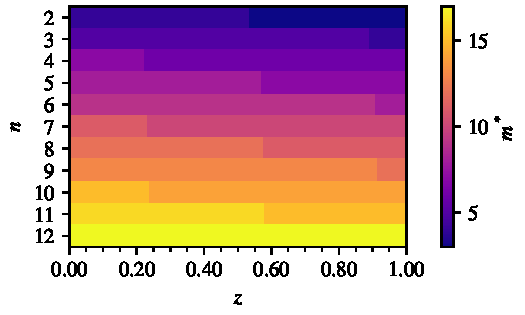
\includegraphics{papers/laguerre/images/targets.pdf}
\caption{$a$ in Abhängigkeit von $z$ und $n$}
\label{laguerre:fig:targets}
\end{figure}


\begin{figure}
\centering
%% Creator: Matplotlib, PGF backend
%%
%% To include the figure in your LaTeX document, write
%%   \input{<filename>.pgf}
%%
%% Make sure the required packages are loaded in your preamble
%%   \usepackage{pgf}
%%
%% Also ensure that all the required font packages are loaded; for instance,
%% the lmodern package is sometimes necessary when using math font.
%%   \usepackage{lmodern}
%%
%% Figures using additional raster images can only be included by \input if
%% they are in the same directory as the main LaTeX file. For loading figures
%% from other directories you can use the `import` package
%%   \usepackage{import}
%%
%% and then include the figures with
%%   \import{<path to file>}{<filename>.pgf}
%%
%% Matplotlib used the following preamble
%%   \usepackage{fontspec}
%%   \setmainfont{DejaVuSerif.ttf}[Path=\detokenize{/home/mup/.local/lib/python3.8/site-packages/matplotlib/mpl-data/fonts/ttf/}]
%%   \setsansfont{DejaVuSans.ttf}[Path=\detokenize{/home/mup/.local/lib/python3.8/site-packages/matplotlib/mpl-data/fonts/ttf/}]
%%   \setmonofont{DejaVuSansMono.ttf}[Path=\detokenize{/home/mup/.local/lib/python3.8/site-packages/matplotlib/mpl-data/fonts/ttf/}]
%%
\begingroup%
\makeatletter%
\begin{pgfpicture}%
\pgfpathrectangle{\pgfpointorigin}{\pgfqpoint{5.000000in}{4.000000in}}%
\pgfusepath{use as bounding box, clip}%
\begin{pgfscope}%
\pgfsetbuttcap%
\pgfsetmiterjoin%
\definecolor{currentfill}{rgb}{1.000000,1.000000,1.000000}%
\pgfsetfillcolor{currentfill}%
\pgfsetlinewidth{0.000000pt}%
\definecolor{currentstroke}{rgb}{1.000000,1.000000,1.000000}%
\pgfsetstrokecolor{currentstroke}%
\pgfsetdash{}{0pt}%
\pgfpathmoveto{\pgfqpoint{0.000000in}{0.000000in}}%
\pgfpathlineto{\pgfqpoint{5.000000in}{0.000000in}}%
\pgfpathlineto{\pgfqpoint{5.000000in}{4.000000in}}%
\pgfpathlineto{\pgfqpoint{0.000000in}{4.000000in}}%
\pgfpathlineto{\pgfqpoint{0.000000in}{0.000000in}}%
\pgfpathclose%
\pgfusepath{fill}%
\end{pgfscope}%
\begin{pgfscope}%
\pgfsetbuttcap%
\pgfsetmiterjoin%
\definecolor{currentfill}{rgb}{1.000000,1.000000,1.000000}%
\pgfsetfillcolor{currentfill}%
\pgfsetlinewidth{0.000000pt}%
\definecolor{currentstroke}{rgb}{0.000000,0.000000,0.000000}%
\pgfsetstrokecolor{currentstroke}%
\pgfsetstrokeopacity{0.000000}%
\pgfsetdash{}{0pt}%
\pgfpathmoveto{\pgfqpoint{0.556162in}{2.276777in}}%
\pgfpathlineto{\pgfqpoint{4.958330in}{2.276777in}}%
\pgfpathlineto{\pgfqpoint{4.958330in}{3.958330in}}%
\pgfpathlineto{\pgfqpoint{0.556162in}{3.958330in}}%
\pgfpathlineto{\pgfqpoint{0.556162in}{2.276777in}}%
\pgfpathclose%
\pgfusepath{fill}%
\end{pgfscope}%
\begin{pgfscope}%
\pgfpathrectangle{\pgfqpoint{0.556162in}{2.276777in}}{\pgfqpoint{4.402168in}{1.681553in}}%
\pgfusepath{clip}%
\pgfsetrectcap%
\pgfsetroundjoin%
\pgfsetlinewidth{0.803000pt}%
\definecolor{currentstroke}{rgb}{0.690196,0.690196,0.690196}%
\pgfsetstrokecolor{currentstroke}%
\pgfsetdash{}{0pt}%
\pgfpathmoveto{\pgfqpoint{0.756261in}{2.276777in}}%
\pgfpathlineto{\pgfqpoint{0.756261in}{3.958330in}}%
\pgfusepath{stroke}%
\end{pgfscope}%
\begin{pgfscope}%
\pgfsetbuttcap%
\pgfsetroundjoin%
\definecolor{currentfill}{rgb}{0.000000,0.000000,0.000000}%
\pgfsetfillcolor{currentfill}%
\pgfsetlinewidth{0.803000pt}%
\definecolor{currentstroke}{rgb}{0.000000,0.000000,0.000000}%
\pgfsetstrokecolor{currentstroke}%
\pgfsetdash{}{0pt}%
\pgfsys@defobject{currentmarker}{\pgfqpoint{0.000000in}{-0.048611in}}{\pgfqpoint{0.000000in}{0.000000in}}{%
\pgfpathmoveto{\pgfqpoint{0.000000in}{0.000000in}}%
\pgfpathlineto{\pgfqpoint{0.000000in}{-0.048611in}}%
\pgfusepath{stroke,fill}%
}%
\begin{pgfscope}%
\pgfsys@transformshift{0.756261in}{2.276777in}%
\pgfsys@useobject{currentmarker}{}%
\end{pgfscope}%
\end{pgfscope}%
\begin{pgfscope}%
\pgfpathrectangle{\pgfqpoint{0.556162in}{2.276777in}}{\pgfqpoint{4.402168in}{1.681553in}}%
\pgfusepath{clip}%
\pgfsetrectcap%
\pgfsetroundjoin%
\pgfsetlinewidth{0.803000pt}%
\definecolor{currentstroke}{rgb}{0.690196,0.690196,0.690196}%
\pgfsetstrokecolor{currentstroke}%
\pgfsetdash{}{0pt}%
\pgfpathmoveto{\pgfqpoint{1.556655in}{2.276777in}}%
\pgfpathlineto{\pgfqpoint{1.556655in}{3.958330in}}%
\pgfusepath{stroke}%
\end{pgfscope}%
\begin{pgfscope}%
\pgfsetbuttcap%
\pgfsetroundjoin%
\definecolor{currentfill}{rgb}{0.000000,0.000000,0.000000}%
\pgfsetfillcolor{currentfill}%
\pgfsetlinewidth{0.803000pt}%
\definecolor{currentstroke}{rgb}{0.000000,0.000000,0.000000}%
\pgfsetstrokecolor{currentstroke}%
\pgfsetdash{}{0pt}%
\pgfsys@defobject{currentmarker}{\pgfqpoint{0.000000in}{-0.048611in}}{\pgfqpoint{0.000000in}{0.000000in}}{%
\pgfpathmoveto{\pgfqpoint{0.000000in}{0.000000in}}%
\pgfpathlineto{\pgfqpoint{0.000000in}{-0.048611in}}%
\pgfusepath{stroke,fill}%
}%
\begin{pgfscope}%
\pgfsys@transformshift{1.556655in}{2.276777in}%
\pgfsys@useobject{currentmarker}{}%
\end{pgfscope}%
\end{pgfscope}%
\begin{pgfscope}%
\pgfpathrectangle{\pgfqpoint{0.556162in}{2.276777in}}{\pgfqpoint{4.402168in}{1.681553in}}%
\pgfusepath{clip}%
\pgfsetrectcap%
\pgfsetroundjoin%
\pgfsetlinewidth{0.803000pt}%
\definecolor{currentstroke}{rgb}{0.690196,0.690196,0.690196}%
\pgfsetstrokecolor{currentstroke}%
\pgfsetdash{}{0pt}%
\pgfpathmoveto{\pgfqpoint{2.357049in}{2.276777in}}%
\pgfpathlineto{\pgfqpoint{2.357049in}{3.958330in}}%
\pgfusepath{stroke}%
\end{pgfscope}%
\begin{pgfscope}%
\pgfsetbuttcap%
\pgfsetroundjoin%
\definecolor{currentfill}{rgb}{0.000000,0.000000,0.000000}%
\pgfsetfillcolor{currentfill}%
\pgfsetlinewidth{0.803000pt}%
\definecolor{currentstroke}{rgb}{0.000000,0.000000,0.000000}%
\pgfsetstrokecolor{currentstroke}%
\pgfsetdash{}{0pt}%
\pgfsys@defobject{currentmarker}{\pgfqpoint{0.000000in}{-0.048611in}}{\pgfqpoint{0.000000in}{0.000000in}}{%
\pgfpathmoveto{\pgfqpoint{0.000000in}{0.000000in}}%
\pgfpathlineto{\pgfqpoint{0.000000in}{-0.048611in}}%
\pgfusepath{stroke,fill}%
}%
\begin{pgfscope}%
\pgfsys@transformshift{2.357049in}{2.276777in}%
\pgfsys@useobject{currentmarker}{}%
\end{pgfscope}%
\end{pgfscope}%
\begin{pgfscope}%
\pgfpathrectangle{\pgfqpoint{0.556162in}{2.276777in}}{\pgfqpoint{4.402168in}{1.681553in}}%
\pgfusepath{clip}%
\pgfsetrectcap%
\pgfsetroundjoin%
\pgfsetlinewidth{0.803000pt}%
\definecolor{currentstroke}{rgb}{0.690196,0.690196,0.690196}%
\pgfsetstrokecolor{currentstroke}%
\pgfsetdash{}{0pt}%
\pgfpathmoveto{\pgfqpoint{3.157443in}{2.276777in}}%
\pgfpathlineto{\pgfqpoint{3.157443in}{3.958330in}}%
\pgfusepath{stroke}%
\end{pgfscope}%
\begin{pgfscope}%
\pgfsetbuttcap%
\pgfsetroundjoin%
\definecolor{currentfill}{rgb}{0.000000,0.000000,0.000000}%
\pgfsetfillcolor{currentfill}%
\pgfsetlinewidth{0.803000pt}%
\definecolor{currentstroke}{rgb}{0.000000,0.000000,0.000000}%
\pgfsetstrokecolor{currentstroke}%
\pgfsetdash{}{0pt}%
\pgfsys@defobject{currentmarker}{\pgfqpoint{0.000000in}{-0.048611in}}{\pgfqpoint{0.000000in}{0.000000in}}{%
\pgfpathmoveto{\pgfqpoint{0.000000in}{0.000000in}}%
\pgfpathlineto{\pgfqpoint{0.000000in}{-0.048611in}}%
\pgfusepath{stroke,fill}%
}%
\begin{pgfscope}%
\pgfsys@transformshift{3.157443in}{2.276777in}%
\pgfsys@useobject{currentmarker}{}%
\end{pgfscope}%
\end{pgfscope}%
\begin{pgfscope}%
\pgfpathrectangle{\pgfqpoint{0.556162in}{2.276777in}}{\pgfqpoint{4.402168in}{1.681553in}}%
\pgfusepath{clip}%
\pgfsetrectcap%
\pgfsetroundjoin%
\pgfsetlinewidth{0.803000pt}%
\definecolor{currentstroke}{rgb}{0.690196,0.690196,0.690196}%
\pgfsetstrokecolor{currentstroke}%
\pgfsetdash{}{0pt}%
\pgfpathmoveto{\pgfqpoint{3.957837in}{2.276777in}}%
\pgfpathlineto{\pgfqpoint{3.957837in}{3.958330in}}%
\pgfusepath{stroke}%
\end{pgfscope}%
\begin{pgfscope}%
\pgfsetbuttcap%
\pgfsetroundjoin%
\definecolor{currentfill}{rgb}{0.000000,0.000000,0.000000}%
\pgfsetfillcolor{currentfill}%
\pgfsetlinewidth{0.803000pt}%
\definecolor{currentstroke}{rgb}{0.000000,0.000000,0.000000}%
\pgfsetstrokecolor{currentstroke}%
\pgfsetdash{}{0pt}%
\pgfsys@defobject{currentmarker}{\pgfqpoint{0.000000in}{-0.048611in}}{\pgfqpoint{0.000000in}{0.000000in}}{%
\pgfpathmoveto{\pgfqpoint{0.000000in}{0.000000in}}%
\pgfpathlineto{\pgfqpoint{0.000000in}{-0.048611in}}%
\pgfusepath{stroke,fill}%
}%
\begin{pgfscope}%
\pgfsys@transformshift{3.957837in}{2.276777in}%
\pgfsys@useobject{currentmarker}{}%
\end{pgfscope}%
\end{pgfscope}%
\begin{pgfscope}%
\pgfpathrectangle{\pgfqpoint{0.556162in}{2.276777in}}{\pgfqpoint{4.402168in}{1.681553in}}%
\pgfusepath{clip}%
\pgfsetrectcap%
\pgfsetroundjoin%
\pgfsetlinewidth{0.803000pt}%
\definecolor{currentstroke}{rgb}{0.690196,0.690196,0.690196}%
\pgfsetstrokecolor{currentstroke}%
\pgfsetdash{}{0pt}%
\pgfpathmoveto{\pgfqpoint{4.758231in}{2.276777in}}%
\pgfpathlineto{\pgfqpoint{4.758231in}{3.958330in}}%
\pgfusepath{stroke}%
\end{pgfscope}%
\begin{pgfscope}%
\pgfsetbuttcap%
\pgfsetroundjoin%
\definecolor{currentfill}{rgb}{0.000000,0.000000,0.000000}%
\pgfsetfillcolor{currentfill}%
\pgfsetlinewidth{0.803000pt}%
\definecolor{currentstroke}{rgb}{0.000000,0.000000,0.000000}%
\pgfsetstrokecolor{currentstroke}%
\pgfsetdash{}{0pt}%
\pgfsys@defobject{currentmarker}{\pgfqpoint{0.000000in}{-0.048611in}}{\pgfqpoint{0.000000in}{0.000000in}}{%
\pgfpathmoveto{\pgfqpoint{0.000000in}{0.000000in}}%
\pgfpathlineto{\pgfqpoint{0.000000in}{-0.048611in}}%
\pgfusepath{stroke,fill}%
}%
\begin{pgfscope}%
\pgfsys@transformshift{4.758231in}{2.276777in}%
\pgfsys@useobject{currentmarker}{}%
\end{pgfscope}%
\end{pgfscope}%
\begin{pgfscope}%
\pgfpathrectangle{\pgfqpoint{0.556162in}{2.276777in}}{\pgfqpoint{4.402168in}{1.681553in}}%
\pgfusepath{clip}%
\pgfsetrectcap%
\pgfsetroundjoin%
\pgfsetlinewidth{0.803000pt}%
\definecolor{currentstroke}{rgb}{0.690196,0.690196,0.690196}%
\pgfsetstrokecolor{currentstroke}%
\pgfsetdash{}{0pt}%
\pgfpathmoveto{\pgfqpoint{0.556162in}{2.574427in}}%
\pgfpathlineto{\pgfqpoint{4.958330in}{2.574427in}}%
\pgfusepath{stroke}%
\end{pgfscope}%
\begin{pgfscope}%
\pgfsetbuttcap%
\pgfsetroundjoin%
\definecolor{currentfill}{rgb}{0.000000,0.000000,0.000000}%
\pgfsetfillcolor{currentfill}%
\pgfsetlinewidth{0.803000pt}%
\definecolor{currentstroke}{rgb}{0.000000,0.000000,0.000000}%
\pgfsetstrokecolor{currentstroke}%
\pgfsetdash{}{0pt}%
\pgfsys@defobject{currentmarker}{\pgfqpoint{-0.048611in}{0.000000in}}{\pgfqpoint{-0.000000in}{0.000000in}}{%
\pgfpathmoveto{\pgfqpoint{-0.000000in}{0.000000in}}%
\pgfpathlineto{\pgfqpoint{-0.048611in}{0.000000in}}%
\pgfusepath{stroke,fill}%
}%
\begin{pgfscope}%
\pgfsys@transformshift{0.556162in}{2.574427in}%
\pgfsys@useobject{currentmarker}{}%
\end{pgfscope}%
\end{pgfscope}%
\begin{pgfscope}%
\definecolor{textcolor}{rgb}{0.000000,0.000000,0.000000}%
\pgfsetstrokecolor{textcolor}%
\pgfsetfillcolor{textcolor}%
\pgftext[x=0.370575in, y=2.521666in, left, base]{\color{textcolor}\sffamily\fontsize{10.000000}{12.000000}\selectfont 5}%
\end{pgfscope}%
\begin{pgfscope}%
\pgfpathrectangle{\pgfqpoint{0.556162in}{2.276777in}}{\pgfqpoint{4.402168in}{1.681553in}}%
\pgfusepath{clip}%
\pgfsetrectcap%
\pgfsetroundjoin%
\pgfsetlinewidth{0.803000pt}%
\definecolor{currentstroke}{rgb}{0.690196,0.690196,0.690196}%
\pgfsetstrokecolor{currentstroke}%
\pgfsetdash{}{0pt}%
\pgfpathmoveto{\pgfqpoint{0.556162in}{3.092617in}}%
\pgfpathlineto{\pgfqpoint{4.958330in}{3.092617in}}%
\pgfusepath{stroke}%
\end{pgfscope}%
\begin{pgfscope}%
\pgfsetbuttcap%
\pgfsetroundjoin%
\definecolor{currentfill}{rgb}{0.000000,0.000000,0.000000}%
\pgfsetfillcolor{currentfill}%
\pgfsetlinewidth{0.803000pt}%
\definecolor{currentstroke}{rgb}{0.000000,0.000000,0.000000}%
\pgfsetstrokecolor{currentstroke}%
\pgfsetdash{}{0pt}%
\pgfsys@defobject{currentmarker}{\pgfqpoint{-0.048611in}{0.000000in}}{\pgfqpoint{-0.000000in}{0.000000in}}{%
\pgfpathmoveto{\pgfqpoint{-0.000000in}{0.000000in}}%
\pgfpathlineto{\pgfqpoint{-0.048611in}{0.000000in}}%
\pgfusepath{stroke,fill}%
}%
\begin{pgfscope}%
\pgfsys@transformshift{0.556162in}{3.092617in}%
\pgfsys@useobject{currentmarker}{}%
\end{pgfscope}%
\end{pgfscope}%
\begin{pgfscope}%
\definecolor{textcolor}{rgb}{0.000000,0.000000,0.000000}%
\pgfsetstrokecolor{textcolor}%
\pgfsetfillcolor{textcolor}%
\pgftext[x=0.282209in, y=3.039855in, left, base]{\color{textcolor}\sffamily\fontsize{10.000000}{12.000000}\selectfont 10}%
\end{pgfscope}%
\begin{pgfscope}%
\pgfpathrectangle{\pgfqpoint{0.556162in}{2.276777in}}{\pgfqpoint{4.402168in}{1.681553in}}%
\pgfusepath{clip}%
\pgfsetrectcap%
\pgfsetroundjoin%
\pgfsetlinewidth{0.803000pt}%
\definecolor{currentstroke}{rgb}{0.690196,0.690196,0.690196}%
\pgfsetstrokecolor{currentstroke}%
\pgfsetdash{}{0pt}%
\pgfpathmoveto{\pgfqpoint{0.556162in}{3.610806in}}%
\pgfpathlineto{\pgfqpoint{4.958330in}{3.610806in}}%
\pgfusepath{stroke}%
\end{pgfscope}%
\begin{pgfscope}%
\pgfsetbuttcap%
\pgfsetroundjoin%
\definecolor{currentfill}{rgb}{0.000000,0.000000,0.000000}%
\pgfsetfillcolor{currentfill}%
\pgfsetlinewidth{0.803000pt}%
\definecolor{currentstroke}{rgb}{0.000000,0.000000,0.000000}%
\pgfsetstrokecolor{currentstroke}%
\pgfsetdash{}{0pt}%
\pgfsys@defobject{currentmarker}{\pgfqpoint{-0.048611in}{0.000000in}}{\pgfqpoint{-0.000000in}{0.000000in}}{%
\pgfpathmoveto{\pgfqpoint{-0.000000in}{0.000000in}}%
\pgfpathlineto{\pgfqpoint{-0.048611in}{0.000000in}}%
\pgfusepath{stroke,fill}%
}%
\begin{pgfscope}%
\pgfsys@transformshift{0.556162in}{3.610806in}%
\pgfsys@useobject{currentmarker}{}%
\end{pgfscope}%
\end{pgfscope}%
\begin{pgfscope}%
\definecolor{textcolor}{rgb}{0.000000,0.000000,0.000000}%
\pgfsetstrokecolor{textcolor}%
\pgfsetfillcolor{textcolor}%
\pgftext[x=0.282209in, y=3.558045in, left, base]{\color{textcolor}\sffamily\fontsize{10.000000}{12.000000}\selectfont 15}%
\end{pgfscope}%
\begin{pgfscope}%
\pgfpathrectangle{\pgfqpoint{0.556162in}{2.276777in}}{\pgfqpoint{4.402168in}{1.681553in}}%
\pgfusepath{clip}%
\pgfsetrectcap%
\pgfsetroundjoin%
\pgfsetlinewidth{1.505625pt}%
\definecolor{currentstroke}{rgb}{0.121569,0.466667,0.705882}%
\pgfsetstrokecolor{currentstroke}%
\pgfsetdash{}{0pt}%
\pgfpathmoveto{\pgfqpoint{0.556162in}{2.353211in}}%
\pgfpathlineto{\pgfqpoint{4.958330in}{3.881896in}}%
\pgfusepath{stroke}%
\end{pgfscope}%
\begin{pgfscope}%
\pgfpathrectangle{\pgfqpoint{0.556162in}{2.276777in}}{\pgfqpoint{4.402168in}{1.681553in}}%
\pgfusepath{clip}%
\pgfsetbuttcap%
\pgfsetroundjoin%
\definecolor{currentfill}{rgb}{1.000000,0.498039,0.054902}%
\pgfsetfillcolor{currentfill}%
\pgfsetlinewidth{1.003750pt}%
\definecolor{currentstroke}{rgb}{1.000000,0.498039,0.054902}%
\pgfsetstrokecolor{currentstroke}%
\pgfsetdash{}{0pt}%
\pgfsys@defobject{currentmarker}{\pgfqpoint{-0.041667in}{-0.041667in}}{\pgfqpoint{0.041667in}{0.041667in}}{%
\pgfpathmoveto{\pgfqpoint{-0.041667in}{-0.041667in}}%
\pgfpathlineto{\pgfqpoint{0.041667in}{0.041667in}}%
\pgfpathmoveto{\pgfqpoint{-0.041667in}{0.041667in}}%
\pgfpathlineto{\pgfqpoint{0.041667in}{-0.041667in}}%
\pgfusepath{stroke,fill}%
}%
\begin{pgfscope}%
\pgfsys@transformshift{0.756261in}{2.422322in}%
\pgfsys@useobject{currentmarker}{}%
\end{pgfscope}%
\begin{pgfscope}%
\pgfsys@transformshift{1.156458in}{2.562568in}%
\pgfsys@useobject{currentmarker}{}%
\end{pgfscope}%
\begin{pgfscope}%
\pgfsys@transformshift{1.556655in}{2.701268in}%
\pgfsys@useobject{currentmarker}{}%
\end{pgfscope}%
\begin{pgfscope}%
\pgfsys@transformshift{1.956852in}{2.840483in}%
\pgfsys@useobject{currentmarker}{}%
\end{pgfscope}%
\begin{pgfscope}%
\pgfsys@transformshift{2.357049in}{2.979182in}%
\pgfsys@useobject{currentmarker}{}%
\end{pgfscope}%
\begin{pgfscope}%
\pgfsys@transformshift{2.757246in}{3.116851in}%
\pgfsys@useobject{currentmarker}{}%
\end{pgfscope}%
\begin{pgfscope}%
\pgfsys@transformshift{3.157443in}{3.255550in}%
\pgfsys@useobject{currentmarker}{}%
\end{pgfscope}%
\begin{pgfscope}%
\pgfsys@transformshift{3.557640in}{3.394249in}%
\pgfsys@useobject{currentmarker}{}%
\end{pgfscope}%
\begin{pgfscope}%
\pgfsys@transformshift{3.957837in}{3.531918in}%
\pgfsys@useobject{currentmarker}{}%
\end{pgfscope}%
\begin{pgfscope}%
\pgfsys@transformshift{4.358034in}{3.670617in}%
\pgfsys@useobject{currentmarker}{}%
\end{pgfscope}%
\begin{pgfscope}%
\pgfsys@transformshift{4.758231in}{3.818082in}%
\pgfsys@useobject{currentmarker}{}%
\end{pgfscope}%
\end{pgfscope}%
\begin{pgfscope}%
\pgfsetrectcap%
\pgfsetmiterjoin%
\pgfsetlinewidth{0.803000pt}%
\definecolor{currentstroke}{rgb}{0.000000,0.000000,0.000000}%
\pgfsetstrokecolor{currentstroke}%
\pgfsetdash{}{0pt}%
\pgfpathmoveto{\pgfqpoint{0.556162in}{2.276777in}}%
\pgfpathlineto{\pgfqpoint{0.556162in}{3.958330in}}%
\pgfusepath{stroke}%
\end{pgfscope}%
\begin{pgfscope}%
\pgfsetrectcap%
\pgfsetmiterjoin%
\pgfsetlinewidth{0.803000pt}%
\definecolor{currentstroke}{rgb}{0.000000,0.000000,0.000000}%
\pgfsetstrokecolor{currentstroke}%
\pgfsetdash{}{0pt}%
\pgfpathmoveto{\pgfqpoint{4.958330in}{2.276777in}}%
\pgfpathlineto{\pgfqpoint{4.958330in}{3.958330in}}%
\pgfusepath{stroke}%
\end{pgfscope}%
\begin{pgfscope}%
\pgfsetrectcap%
\pgfsetmiterjoin%
\pgfsetlinewidth{0.803000pt}%
\definecolor{currentstroke}{rgb}{0.000000,0.000000,0.000000}%
\pgfsetstrokecolor{currentstroke}%
\pgfsetdash{}{0pt}%
\pgfpathmoveto{\pgfqpoint{0.556162in}{2.276777in}}%
\pgfpathlineto{\pgfqpoint{4.958330in}{2.276777in}}%
\pgfusepath{stroke}%
\end{pgfscope}%
\begin{pgfscope}%
\pgfsetrectcap%
\pgfsetmiterjoin%
\pgfsetlinewidth{0.803000pt}%
\definecolor{currentstroke}{rgb}{0.000000,0.000000,0.000000}%
\pgfsetstrokecolor{currentstroke}%
\pgfsetdash{}{0pt}%
\pgfpathmoveto{\pgfqpoint{0.556162in}{3.958330in}}%
\pgfpathlineto{\pgfqpoint{4.958330in}{3.958330in}}%
\pgfusepath{stroke}%
\end{pgfscope}%
\begin{pgfscope}%
\pgfsetbuttcap%
\pgfsetmiterjoin%
\definecolor{currentfill}{rgb}{1.000000,1.000000,1.000000}%
\pgfsetfillcolor{currentfill}%
\pgfsetfillopacity{0.800000}%
\pgfsetlinewidth{1.003750pt}%
\definecolor{currentstroke}{rgb}{0.800000,0.800000,0.800000}%
\pgfsetstrokecolor{currentstroke}%
\pgfsetstrokeopacity{0.800000}%
\pgfsetdash{}{0pt}%
\pgfpathmoveto{\pgfqpoint{0.653384in}{3.439504in}}%
\pgfpathlineto{\pgfqpoint{1.219775in}{3.439504in}}%
\pgfpathquadraticcurveto{\pgfqpoint{1.247553in}{3.439504in}}{\pgfqpoint{1.247553in}{3.467282in}}%
\pgfpathlineto{\pgfqpoint{1.247553in}{3.861108in}}%
\pgfpathquadraticcurveto{\pgfqpoint{1.247553in}{3.888886in}}{\pgfqpoint{1.219775in}{3.888886in}}%
\pgfpathlineto{\pgfqpoint{0.653384in}{3.888886in}}%
\pgfpathquadraticcurveto{\pgfqpoint{0.625607in}{3.888886in}}{\pgfqpoint{0.625607in}{3.861108in}}%
\pgfpathlineto{\pgfqpoint{0.625607in}{3.467282in}}%
\pgfpathquadraticcurveto{\pgfqpoint{0.625607in}{3.439504in}}{\pgfqpoint{0.653384in}{3.439504in}}%
\pgfpathlineto{\pgfqpoint{0.653384in}{3.439504in}}%
\pgfpathclose%
\pgfusepath{stroke,fill}%
\end{pgfscope}%
\begin{pgfscope}%
\pgfsetrectcap%
\pgfsetroundjoin%
\pgfsetlinewidth{1.505625pt}%
\definecolor{currentstroke}{rgb}{0.121569,0.466667,0.705882}%
\pgfsetstrokecolor{currentstroke}%
\pgfsetdash{}{0pt}%
\pgfpathmoveto{\pgfqpoint{0.681162in}{3.776418in}}%
\pgfpathlineto{\pgfqpoint{0.820051in}{3.776418in}}%
\pgfpathlineto{\pgfqpoint{0.958940in}{3.776418in}}%
\pgfusepath{stroke}%
\end{pgfscope}%
\begin{pgfscope}%
\definecolor{textcolor}{rgb}{0.000000,0.000000,0.000000}%
\pgfsetstrokecolor{textcolor}%
\pgfsetfillcolor{textcolor}%
\pgftext[x=1.070051in,y=3.727807in,left,base]{\color{textcolor}\sffamily\fontsize{10.000000}{12.000000}\selectfont \(\displaystyle \hat{m}\)}%
\end{pgfscope}%
\begin{pgfscope}%
\pgfsetbuttcap%
\pgfsetroundjoin%
\definecolor{currentfill}{rgb}{1.000000,0.498039,0.054902}%
\pgfsetfillcolor{currentfill}%
\pgfsetlinewidth{1.003750pt}%
\definecolor{currentstroke}{rgb}{1.000000,0.498039,0.054902}%
\pgfsetstrokecolor{currentstroke}%
\pgfsetdash{}{0pt}%
\pgfsys@defobject{currentmarker}{\pgfqpoint{-0.041667in}{-0.041667in}}{\pgfqpoint{0.041667in}{0.041667in}}{%
\pgfpathmoveto{\pgfqpoint{-0.041667in}{-0.041667in}}%
\pgfpathlineto{\pgfqpoint{0.041667in}{0.041667in}}%
\pgfpathmoveto{\pgfqpoint{-0.041667in}{0.041667in}}%
\pgfpathlineto{\pgfqpoint{0.041667in}{-0.041667in}}%
\pgfusepath{stroke,fill}%
}%
\begin{pgfscope}%
\pgfsys@transformshift{0.820051in}{3.572561in}%
\pgfsys@useobject{currentmarker}{}%
\end{pgfscope}%
\end{pgfscope}%
\begin{pgfscope}%
\definecolor{textcolor}{rgb}{0.000000,0.000000,0.000000}%
\pgfsetstrokecolor{textcolor}%
\pgfsetfillcolor{textcolor}%
\pgftext[x=1.070051in,y=3.523950in,left,base]{\color{textcolor}\sffamily\fontsize{10.000000}{12.000000}\selectfont \(\displaystyle \overline{m}\)}%
\end{pgfscope}%
\begin{pgfscope}%
\pgfsetbuttcap%
\pgfsetmiterjoin%
\definecolor{currentfill}{rgb}{1.000000,1.000000,1.000000}%
\pgfsetfillcolor{currentfill}%
\pgfsetlinewidth{0.000000pt}%
\definecolor{currentstroke}{rgb}{0.000000,0.000000,0.000000}%
\pgfsetstrokecolor{currentstroke}%
\pgfsetstrokeopacity{0.000000}%
\pgfsetdash{}{0pt}%
\pgfpathmoveto{\pgfqpoint{0.556162in}{0.463273in}}%
\pgfpathlineto{\pgfqpoint{4.958330in}{0.463273in}}%
\pgfpathlineto{\pgfqpoint{4.958330in}{2.144826in}}%
\pgfpathlineto{\pgfqpoint{0.556162in}{2.144826in}}%
\pgfpathlineto{\pgfqpoint{0.556162in}{0.463273in}}%
\pgfpathclose%
\pgfusepath{fill}%
\end{pgfscope}%
\begin{pgfscope}%
\pgfpathrectangle{\pgfqpoint{0.556162in}{0.463273in}}{\pgfqpoint{4.402168in}{1.681553in}}%
\pgfusepath{clip}%
\pgfsetrectcap%
\pgfsetroundjoin%
\pgfsetlinewidth{0.803000pt}%
\definecolor{currentstroke}{rgb}{0.690196,0.690196,0.690196}%
\pgfsetstrokecolor{currentstroke}%
\pgfsetdash{}{0pt}%
\pgfpathmoveto{\pgfqpoint{0.756261in}{0.463273in}}%
\pgfpathlineto{\pgfqpoint{0.756261in}{2.144826in}}%
\pgfusepath{stroke}%
\end{pgfscope}%
\begin{pgfscope}%
\pgfsetbuttcap%
\pgfsetroundjoin%
\definecolor{currentfill}{rgb}{0.000000,0.000000,0.000000}%
\pgfsetfillcolor{currentfill}%
\pgfsetlinewidth{0.803000pt}%
\definecolor{currentstroke}{rgb}{0.000000,0.000000,0.000000}%
\pgfsetstrokecolor{currentstroke}%
\pgfsetdash{}{0pt}%
\pgfsys@defobject{currentmarker}{\pgfqpoint{0.000000in}{-0.048611in}}{\pgfqpoint{0.000000in}{0.000000in}}{%
\pgfpathmoveto{\pgfqpoint{0.000000in}{0.000000in}}%
\pgfpathlineto{\pgfqpoint{0.000000in}{-0.048611in}}%
\pgfusepath{stroke,fill}%
}%
\begin{pgfscope}%
\pgfsys@transformshift{0.756261in}{0.463273in}%
\pgfsys@useobject{currentmarker}{}%
\end{pgfscope}%
\end{pgfscope}%
\begin{pgfscope}%
\definecolor{textcolor}{rgb}{0.000000,0.000000,0.000000}%
\pgfsetstrokecolor{textcolor}%
\pgfsetfillcolor{textcolor}%
\pgftext[x=0.756261in,y=0.366051in,,top]{\color{textcolor}\sffamily\fontsize{10.000000}{12.000000}\selectfont 2}%
\end{pgfscope}%
\begin{pgfscope}%
\pgfpathrectangle{\pgfqpoint{0.556162in}{0.463273in}}{\pgfqpoint{4.402168in}{1.681553in}}%
\pgfusepath{clip}%
\pgfsetrectcap%
\pgfsetroundjoin%
\pgfsetlinewidth{0.803000pt}%
\definecolor{currentstroke}{rgb}{0.690196,0.690196,0.690196}%
\pgfsetstrokecolor{currentstroke}%
\pgfsetdash{}{0pt}%
\pgfpathmoveto{\pgfqpoint{1.556655in}{0.463273in}}%
\pgfpathlineto{\pgfqpoint{1.556655in}{2.144826in}}%
\pgfusepath{stroke}%
\end{pgfscope}%
\begin{pgfscope}%
\pgfsetbuttcap%
\pgfsetroundjoin%
\definecolor{currentfill}{rgb}{0.000000,0.000000,0.000000}%
\pgfsetfillcolor{currentfill}%
\pgfsetlinewidth{0.803000pt}%
\definecolor{currentstroke}{rgb}{0.000000,0.000000,0.000000}%
\pgfsetstrokecolor{currentstroke}%
\pgfsetdash{}{0pt}%
\pgfsys@defobject{currentmarker}{\pgfqpoint{0.000000in}{-0.048611in}}{\pgfqpoint{0.000000in}{0.000000in}}{%
\pgfpathmoveto{\pgfqpoint{0.000000in}{0.000000in}}%
\pgfpathlineto{\pgfqpoint{0.000000in}{-0.048611in}}%
\pgfusepath{stroke,fill}%
}%
\begin{pgfscope}%
\pgfsys@transformshift{1.556655in}{0.463273in}%
\pgfsys@useobject{currentmarker}{}%
\end{pgfscope}%
\end{pgfscope}%
\begin{pgfscope}%
\definecolor{textcolor}{rgb}{0.000000,0.000000,0.000000}%
\pgfsetstrokecolor{textcolor}%
\pgfsetfillcolor{textcolor}%
\pgftext[x=1.556655in,y=0.366051in,,top]{\color{textcolor}\sffamily\fontsize{10.000000}{12.000000}\selectfont 4}%
\end{pgfscope}%
\begin{pgfscope}%
\pgfpathrectangle{\pgfqpoint{0.556162in}{0.463273in}}{\pgfqpoint{4.402168in}{1.681553in}}%
\pgfusepath{clip}%
\pgfsetrectcap%
\pgfsetroundjoin%
\pgfsetlinewidth{0.803000pt}%
\definecolor{currentstroke}{rgb}{0.690196,0.690196,0.690196}%
\pgfsetstrokecolor{currentstroke}%
\pgfsetdash{}{0pt}%
\pgfpathmoveto{\pgfqpoint{2.357049in}{0.463273in}}%
\pgfpathlineto{\pgfqpoint{2.357049in}{2.144826in}}%
\pgfusepath{stroke}%
\end{pgfscope}%
\begin{pgfscope}%
\pgfsetbuttcap%
\pgfsetroundjoin%
\definecolor{currentfill}{rgb}{0.000000,0.000000,0.000000}%
\pgfsetfillcolor{currentfill}%
\pgfsetlinewidth{0.803000pt}%
\definecolor{currentstroke}{rgb}{0.000000,0.000000,0.000000}%
\pgfsetstrokecolor{currentstroke}%
\pgfsetdash{}{0pt}%
\pgfsys@defobject{currentmarker}{\pgfqpoint{0.000000in}{-0.048611in}}{\pgfqpoint{0.000000in}{0.000000in}}{%
\pgfpathmoveto{\pgfqpoint{0.000000in}{0.000000in}}%
\pgfpathlineto{\pgfqpoint{0.000000in}{-0.048611in}}%
\pgfusepath{stroke,fill}%
}%
\begin{pgfscope}%
\pgfsys@transformshift{2.357049in}{0.463273in}%
\pgfsys@useobject{currentmarker}{}%
\end{pgfscope}%
\end{pgfscope}%
\begin{pgfscope}%
\definecolor{textcolor}{rgb}{0.000000,0.000000,0.000000}%
\pgfsetstrokecolor{textcolor}%
\pgfsetfillcolor{textcolor}%
\pgftext[x=2.357049in,y=0.366051in,,top]{\color{textcolor}\sffamily\fontsize{10.000000}{12.000000}\selectfont 6}%
\end{pgfscope}%
\begin{pgfscope}%
\pgfpathrectangle{\pgfqpoint{0.556162in}{0.463273in}}{\pgfqpoint{4.402168in}{1.681553in}}%
\pgfusepath{clip}%
\pgfsetrectcap%
\pgfsetroundjoin%
\pgfsetlinewidth{0.803000pt}%
\definecolor{currentstroke}{rgb}{0.690196,0.690196,0.690196}%
\pgfsetstrokecolor{currentstroke}%
\pgfsetdash{}{0pt}%
\pgfpathmoveto{\pgfqpoint{3.157443in}{0.463273in}}%
\pgfpathlineto{\pgfqpoint{3.157443in}{2.144826in}}%
\pgfusepath{stroke}%
\end{pgfscope}%
\begin{pgfscope}%
\pgfsetbuttcap%
\pgfsetroundjoin%
\definecolor{currentfill}{rgb}{0.000000,0.000000,0.000000}%
\pgfsetfillcolor{currentfill}%
\pgfsetlinewidth{0.803000pt}%
\definecolor{currentstroke}{rgb}{0.000000,0.000000,0.000000}%
\pgfsetstrokecolor{currentstroke}%
\pgfsetdash{}{0pt}%
\pgfsys@defobject{currentmarker}{\pgfqpoint{0.000000in}{-0.048611in}}{\pgfqpoint{0.000000in}{0.000000in}}{%
\pgfpathmoveto{\pgfqpoint{0.000000in}{0.000000in}}%
\pgfpathlineto{\pgfqpoint{0.000000in}{-0.048611in}}%
\pgfusepath{stroke,fill}%
}%
\begin{pgfscope}%
\pgfsys@transformshift{3.157443in}{0.463273in}%
\pgfsys@useobject{currentmarker}{}%
\end{pgfscope}%
\end{pgfscope}%
\begin{pgfscope}%
\definecolor{textcolor}{rgb}{0.000000,0.000000,0.000000}%
\pgfsetstrokecolor{textcolor}%
\pgfsetfillcolor{textcolor}%
\pgftext[x=3.157443in,y=0.366051in,,top]{\color{textcolor}\sffamily\fontsize{10.000000}{12.000000}\selectfont 8}%
\end{pgfscope}%
\begin{pgfscope}%
\pgfpathrectangle{\pgfqpoint{0.556162in}{0.463273in}}{\pgfqpoint{4.402168in}{1.681553in}}%
\pgfusepath{clip}%
\pgfsetrectcap%
\pgfsetroundjoin%
\pgfsetlinewidth{0.803000pt}%
\definecolor{currentstroke}{rgb}{0.690196,0.690196,0.690196}%
\pgfsetstrokecolor{currentstroke}%
\pgfsetdash{}{0pt}%
\pgfpathmoveto{\pgfqpoint{3.957837in}{0.463273in}}%
\pgfpathlineto{\pgfqpoint{3.957837in}{2.144826in}}%
\pgfusepath{stroke}%
\end{pgfscope}%
\begin{pgfscope}%
\pgfsetbuttcap%
\pgfsetroundjoin%
\definecolor{currentfill}{rgb}{0.000000,0.000000,0.000000}%
\pgfsetfillcolor{currentfill}%
\pgfsetlinewidth{0.803000pt}%
\definecolor{currentstroke}{rgb}{0.000000,0.000000,0.000000}%
\pgfsetstrokecolor{currentstroke}%
\pgfsetdash{}{0pt}%
\pgfsys@defobject{currentmarker}{\pgfqpoint{0.000000in}{-0.048611in}}{\pgfqpoint{0.000000in}{0.000000in}}{%
\pgfpathmoveto{\pgfqpoint{0.000000in}{0.000000in}}%
\pgfpathlineto{\pgfqpoint{0.000000in}{-0.048611in}}%
\pgfusepath{stroke,fill}%
}%
\begin{pgfscope}%
\pgfsys@transformshift{3.957837in}{0.463273in}%
\pgfsys@useobject{currentmarker}{}%
\end{pgfscope}%
\end{pgfscope}%
\begin{pgfscope}%
\definecolor{textcolor}{rgb}{0.000000,0.000000,0.000000}%
\pgfsetstrokecolor{textcolor}%
\pgfsetfillcolor{textcolor}%
\pgftext[x=3.957837in,y=0.366051in,,top]{\color{textcolor}\sffamily\fontsize{10.000000}{12.000000}\selectfont 10}%
\end{pgfscope}%
\begin{pgfscope}%
\pgfpathrectangle{\pgfqpoint{0.556162in}{0.463273in}}{\pgfqpoint{4.402168in}{1.681553in}}%
\pgfusepath{clip}%
\pgfsetrectcap%
\pgfsetroundjoin%
\pgfsetlinewidth{0.803000pt}%
\definecolor{currentstroke}{rgb}{0.690196,0.690196,0.690196}%
\pgfsetstrokecolor{currentstroke}%
\pgfsetdash{}{0pt}%
\pgfpathmoveto{\pgfqpoint{4.758231in}{0.463273in}}%
\pgfpathlineto{\pgfqpoint{4.758231in}{2.144826in}}%
\pgfusepath{stroke}%
\end{pgfscope}%
\begin{pgfscope}%
\pgfsetbuttcap%
\pgfsetroundjoin%
\definecolor{currentfill}{rgb}{0.000000,0.000000,0.000000}%
\pgfsetfillcolor{currentfill}%
\pgfsetlinewidth{0.803000pt}%
\definecolor{currentstroke}{rgb}{0.000000,0.000000,0.000000}%
\pgfsetstrokecolor{currentstroke}%
\pgfsetdash{}{0pt}%
\pgfsys@defobject{currentmarker}{\pgfqpoint{0.000000in}{-0.048611in}}{\pgfqpoint{0.000000in}{0.000000in}}{%
\pgfpathmoveto{\pgfqpoint{0.000000in}{0.000000in}}%
\pgfpathlineto{\pgfqpoint{0.000000in}{-0.048611in}}%
\pgfusepath{stroke,fill}%
}%
\begin{pgfscope}%
\pgfsys@transformshift{4.758231in}{0.463273in}%
\pgfsys@useobject{currentmarker}{}%
\end{pgfscope}%
\end{pgfscope}%
\begin{pgfscope}%
\definecolor{textcolor}{rgb}{0.000000,0.000000,0.000000}%
\pgfsetstrokecolor{textcolor}%
\pgfsetfillcolor{textcolor}%
\pgftext[x=4.758231in,y=0.366051in,,top]{\color{textcolor}\sffamily\fontsize{10.000000}{12.000000}\selectfont 12}%
\end{pgfscope}%
\begin{pgfscope}%
\definecolor{textcolor}{rgb}{0.000000,0.000000,0.000000}%
\pgfsetstrokecolor{textcolor}%
\pgfsetfillcolor{textcolor}%
\pgftext[x=2.757246in,y=0.176083in,,top]{\color{textcolor}\sffamily\fontsize{10.000000}{12.000000}\selectfont \(\displaystyle n\)}%
\end{pgfscope}%
\begin{pgfscope}%
\pgfpathrectangle{\pgfqpoint{0.556162in}{0.463273in}}{\pgfqpoint{4.402168in}{1.681553in}}%
\pgfusepath{clip}%
\pgfsetrectcap%
\pgfsetroundjoin%
\pgfsetlinewidth{0.803000pt}%
\definecolor{currentstroke}{rgb}{0.690196,0.690196,0.690196}%
\pgfsetstrokecolor{currentstroke}%
\pgfsetdash{}{0pt}%
\pgfpathmoveto{\pgfqpoint{0.556162in}{0.814398in}}%
\pgfpathlineto{\pgfqpoint{4.958330in}{0.814398in}}%
\pgfusepath{stroke}%
\end{pgfscope}%
\begin{pgfscope}%
\pgfsetbuttcap%
\pgfsetroundjoin%
\definecolor{currentfill}{rgb}{0.000000,0.000000,0.000000}%
\pgfsetfillcolor{currentfill}%
\pgfsetlinewidth{0.803000pt}%
\definecolor{currentstroke}{rgb}{0.000000,0.000000,0.000000}%
\pgfsetstrokecolor{currentstroke}%
\pgfsetdash{}{0pt}%
\pgfsys@defobject{currentmarker}{\pgfqpoint{-0.048611in}{0.000000in}}{\pgfqpoint{-0.000000in}{0.000000in}}{%
\pgfpathmoveto{\pgfqpoint{-0.000000in}{0.000000in}}%
\pgfpathlineto{\pgfqpoint{-0.048611in}{0.000000in}}%
\pgfusepath{stroke,fill}%
}%
\begin{pgfscope}%
\pgfsys@transformshift{0.556162in}{0.814398in}%
\pgfsys@useobject{currentmarker}{}%
\end{pgfscope}%
\end{pgfscope}%
\begin{pgfscope}%
\definecolor{textcolor}{rgb}{0.000000,0.000000,0.000000}%
\pgfsetstrokecolor{textcolor}%
\pgfsetfillcolor{textcolor}%
\pgftext[x=0.041670in, y=0.761637in, left, base]{\color{textcolor}\sffamily\fontsize{10.000000}{12.000000}\selectfont \ensuremath{-}0.04}%
\end{pgfscope}%
\begin{pgfscope}%
\pgfpathrectangle{\pgfqpoint{0.556162in}{0.463273in}}{\pgfqpoint{4.402168in}{1.681553in}}%
\pgfusepath{clip}%
\pgfsetrectcap%
\pgfsetroundjoin%
\pgfsetlinewidth{0.803000pt}%
\definecolor{currentstroke}{rgb}{0.690196,0.690196,0.690196}%
\pgfsetstrokecolor{currentstroke}%
\pgfsetdash{}{0pt}%
\pgfpathmoveto{\pgfqpoint{0.556162in}{1.187458in}}%
\pgfpathlineto{\pgfqpoint{4.958330in}{1.187458in}}%
\pgfusepath{stroke}%
\end{pgfscope}%
\begin{pgfscope}%
\pgfsetbuttcap%
\pgfsetroundjoin%
\definecolor{currentfill}{rgb}{0.000000,0.000000,0.000000}%
\pgfsetfillcolor{currentfill}%
\pgfsetlinewidth{0.803000pt}%
\definecolor{currentstroke}{rgb}{0.000000,0.000000,0.000000}%
\pgfsetstrokecolor{currentstroke}%
\pgfsetdash{}{0pt}%
\pgfsys@defobject{currentmarker}{\pgfqpoint{-0.048611in}{0.000000in}}{\pgfqpoint{-0.000000in}{0.000000in}}{%
\pgfpathmoveto{\pgfqpoint{-0.000000in}{0.000000in}}%
\pgfpathlineto{\pgfqpoint{-0.048611in}{0.000000in}}%
\pgfusepath{stroke,fill}%
}%
\begin{pgfscope}%
\pgfsys@transformshift{0.556162in}{1.187458in}%
\pgfsys@useobject{currentmarker}{}%
\end{pgfscope}%
\end{pgfscope}%
\begin{pgfscope}%
\definecolor{textcolor}{rgb}{0.000000,0.000000,0.000000}%
\pgfsetstrokecolor{textcolor}%
\pgfsetfillcolor{textcolor}%
\pgftext[x=0.041670in, y=1.134696in, left, base]{\color{textcolor}\sffamily\fontsize{10.000000}{12.000000}\selectfont \ensuremath{-}0.02}%
\end{pgfscope}%
\begin{pgfscope}%
\pgfpathrectangle{\pgfqpoint{0.556162in}{0.463273in}}{\pgfqpoint{4.402168in}{1.681553in}}%
\pgfusepath{clip}%
\pgfsetrectcap%
\pgfsetroundjoin%
\pgfsetlinewidth{0.803000pt}%
\definecolor{currentstroke}{rgb}{0.690196,0.690196,0.690196}%
\pgfsetstrokecolor{currentstroke}%
\pgfsetdash{}{0pt}%
\pgfpathmoveto{\pgfqpoint{0.556162in}{1.560518in}}%
\pgfpathlineto{\pgfqpoint{4.958330in}{1.560518in}}%
\pgfusepath{stroke}%
\end{pgfscope}%
\begin{pgfscope}%
\pgfsetbuttcap%
\pgfsetroundjoin%
\definecolor{currentfill}{rgb}{0.000000,0.000000,0.000000}%
\pgfsetfillcolor{currentfill}%
\pgfsetlinewidth{0.803000pt}%
\definecolor{currentstroke}{rgb}{0.000000,0.000000,0.000000}%
\pgfsetstrokecolor{currentstroke}%
\pgfsetdash{}{0pt}%
\pgfsys@defobject{currentmarker}{\pgfqpoint{-0.048611in}{0.000000in}}{\pgfqpoint{-0.000000in}{0.000000in}}{%
\pgfpathmoveto{\pgfqpoint{-0.000000in}{0.000000in}}%
\pgfpathlineto{\pgfqpoint{-0.048611in}{0.000000in}}%
\pgfusepath{stroke,fill}%
}%
\begin{pgfscope}%
\pgfsys@transformshift{0.556162in}{1.560518in}%
\pgfsys@useobject{currentmarker}{}%
\end{pgfscope}%
\end{pgfscope}%
\begin{pgfscope}%
\definecolor{textcolor}{rgb}{0.000000,0.000000,0.000000}%
\pgfsetstrokecolor{textcolor}%
\pgfsetfillcolor{textcolor}%
\pgftext[x=0.149695in, y=1.507756in, left, base]{\color{textcolor}\sffamily\fontsize{10.000000}{12.000000}\selectfont 0.00}%
\end{pgfscope}%
\begin{pgfscope}%
\pgfpathrectangle{\pgfqpoint{0.556162in}{0.463273in}}{\pgfqpoint{4.402168in}{1.681553in}}%
\pgfusepath{clip}%
\pgfsetrectcap%
\pgfsetroundjoin%
\pgfsetlinewidth{0.803000pt}%
\definecolor{currentstroke}{rgb}{0.690196,0.690196,0.690196}%
\pgfsetstrokecolor{currentstroke}%
\pgfsetdash{}{0pt}%
\pgfpathmoveto{\pgfqpoint{0.556162in}{1.933577in}}%
\pgfpathlineto{\pgfqpoint{4.958330in}{1.933577in}}%
\pgfusepath{stroke}%
\end{pgfscope}%
\begin{pgfscope}%
\pgfsetbuttcap%
\pgfsetroundjoin%
\definecolor{currentfill}{rgb}{0.000000,0.000000,0.000000}%
\pgfsetfillcolor{currentfill}%
\pgfsetlinewidth{0.803000pt}%
\definecolor{currentstroke}{rgb}{0.000000,0.000000,0.000000}%
\pgfsetstrokecolor{currentstroke}%
\pgfsetdash{}{0pt}%
\pgfsys@defobject{currentmarker}{\pgfqpoint{-0.048611in}{0.000000in}}{\pgfqpoint{-0.000000in}{0.000000in}}{%
\pgfpathmoveto{\pgfqpoint{-0.000000in}{0.000000in}}%
\pgfpathlineto{\pgfqpoint{-0.048611in}{0.000000in}}%
\pgfusepath{stroke,fill}%
}%
\begin{pgfscope}%
\pgfsys@transformshift{0.556162in}{1.933577in}%
\pgfsys@useobject{currentmarker}{}%
\end{pgfscope}%
\end{pgfscope}%
\begin{pgfscope}%
\definecolor{textcolor}{rgb}{0.000000,0.000000,0.000000}%
\pgfsetstrokecolor{textcolor}%
\pgfsetfillcolor{textcolor}%
\pgftext[x=0.149695in, y=1.880816in, left, base]{\color{textcolor}\sffamily\fontsize{10.000000}{12.000000}\selectfont 0.02}%
\end{pgfscope}%
\begin{pgfscope}%
\pgfpathrectangle{\pgfqpoint{0.556162in}{0.463273in}}{\pgfqpoint{4.402168in}{1.681553in}}%
\pgfusepath{clip}%
\pgfsetrectcap%
\pgfsetroundjoin%
\pgfsetlinewidth{1.505625pt}%
\definecolor{currentstroke}{rgb}{0.121569,0.466667,0.705882}%
\pgfsetstrokecolor{currentstroke}%
\pgfsetdash{}{0pt}%
\pgfpathmoveto{\pgfqpoint{0.756261in}{1.628009in}}%
\pgfpathlineto{\pgfqpoint{1.156458in}{1.398538in}}%
\pgfpathlineto{\pgfqpoint{1.556655in}{1.447469in}}%
\pgfpathlineto{\pgfqpoint{1.956852in}{1.403600in}}%
\pgfpathlineto{\pgfqpoint{2.357049in}{1.452531in}}%
\pgfpathlineto{\pgfqpoint{2.757246in}{1.687064in}}%
\pgfpathlineto{\pgfqpoint{3.157443in}{1.735996in}}%
\pgfpathlineto{\pgfqpoint{3.557640in}{1.784927in}}%
\pgfpathlineto{\pgfqpoint{3.957837in}{2.019460in}}%
\pgfpathlineto{\pgfqpoint{4.358034in}{2.068392in}}%
\pgfpathlineto{\pgfqpoint{4.758231in}{0.539708in}}%
\pgfusepath{stroke}%
\end{pgfscope}%
\begin{pgfscope}%
\pgfpathrectangle{\pgfqpoint{0.556162in}{0.463273in}}{\pgfqpoint{4.402168in}{1.681553in}}%
\pgfusepath{clip}%
\pgfsetbuttcap%
\pgfsetroundjoin%
\definecolor{currentfill}{rgb}{0.121569,0.466667,0.705882}%
\pgfsetfillcolor{currentfill}%
\pgfsetlinewidth{1.003750pt}%
\definecolor{currentstroke}{rgb}{0.121569,0.466667,0.705882}%
\pgfsetstrokecolor{currentstroke}%
\pgfsetdash{}{0pt}%
\pgfsys@defobject{currentmarker}{\pgfqpoint{-0.041667in}{-0.041667in}}{\pgfqpoint{0.041667in}{0.041667in}}{%
\pgfpathmoveto{\pgfqpoint{-0.041667in}{-0.041667in}}%
\pgfpathlineto{\pgfqpoint{0.041667in}{0.041667in}}%
\pgfpathmoveto{\pgfqpoint{-0.041667in}{0.041667in}}%
\pgfpathlineto{\pgfqpoint{0.041667in}{-0.041667in}}%
\pgfusepath{stroke,fill}%
}%
\begin{pgfscope}%
\pgfsys@transformshift{0.756261in}{1.628009in}%
\pgfsys@useobject{currentmarker}{}%
\end{pgfscope}%
\begin{pgfscope}%
\pgfsys@transformshift{1.156458in}{1.398538in}%
\pgfsys@useobject{currentmarker}{}%
\end{pgfscope}%
\begin{pgfscope}%
\pgfsys@transformshift{1.556655in}{1.447469in}%
\pgfsys@useobject{currentmarker}{}%
\end{pgfscope}%
\begin{pgfscope}%
\pgfsys@transformshift{1.956852in}{1.403600in}%
\pgfsys@useobject{currentmarker}{}%
\end{pgfscope}%
\begin{pgfscope}%
\pgfsys@transformshift{2.357049in}{1.452531in}%
\pgfsys@useobject{currentmarker}{}%
\end{pgfscope}%
\begin{pgfscope}%
\pgfsys@transformshift{2.757246in}{1.687064in}%
\pgfsys@useobject{currentmarker}{}%
\end{pgfscope}%
\begin{pgfscope}%
\pgfsys@transformshift{3.157443in}{1.735996in}%
\pgfsys@useobject{currentmarker}{}%
\end{pgfscope}%
\begin{pgfscope}%
\pgfsys@transformshift{3.557640in}{1.784927in}%
\pgfsys@useobject{currentmarker}{}%
\end{pgfscope}%
\begin{pgfscope}%
\pgfsys@transformshift{3.957837in}{2.019460in}%
\pgfsys@useobject{currentmarker}{}%
\end{pgfscope}%
\begin{pgfscope}%
\pgfsys@transformshift{4.358034in}{2.068392in}%
\pgfsys@useobject{currentmarker}{}%
\end{pgfscope}%
\begin{pgfscope}%
\pgfsys@transformshift{4.758231in}{0.539708in}%
\pgfsys@useobject{currentmarker}{}%
\end{pgfscope}%
\end{pgfscope}%
\begin{pgfscope}%
\pgfsetrectcap%
\pgfsetmiterjoin%
\pgfsetlinewidth{0.803000pt}%
\definecolor{currentstroke}{rgb}{0.000000,0.000000,0.000000}%
\pgfsetstrokecolor{currentstroke}%
\pgfsetdash{}{0pt}%
\pgfpathmoveto{\pgfqpoint{0.556162in}{0.463273in}}%
\pgfpathlineto{\pgfqpoint{0.556162in}{2.144826in}}%
\pgfusepath{stroke}%
\end{pgfscope}%
\begin{pgfscope}%
\pgfsetrectcap%
\pgfsetmiterjoin%
\pgfsetlinewidth{0.803000pt}%
\definecolor{currentstroke}{rgb}{0.000000,0.000000,0.000000}%
\pgfsetstrokecolor{currentstroke}%
\pgfsetdash{}{0pt}%
\pgfpathmoveto{\pgfqpoint{4.958330in}{0.463273in}}%
\pgfpathlineto{\pgfqpoint{4.958330in}{2.144826in}}%
\pgfusepath{stroke}%
\end{pgfscope}%
\begin{pgfscope}%
\pgfsetrectcap%
\pgfsetmiterjoin%
\pgfsetlinewidth{0.803000pt}%
\definecolor{currentstroke}{rgb}{0.000000,0.000000,0.000000}%
\pgfsetstrokecolor{currentstroke}%
\pgfsetdash{}{0pt}%
\pgfpathmoveto{\pgfqpoint{0.556162in}{0.463273in}}%
\pgfpathlineto{\pgfqpoint{4.958330in}{0.463273in}}%
\pgfusepath{stroke}%
\end{pgfscope}%
\begin{pgfscope}%
\pgfsetrectcap%
\pgfsetmiterjoin%
\pgfsetlinewidth{0.803000pt}%
\definecolor{currentstroke}{rgb}{0.000000,0.000000,0.000000}%
\pgfsetstrokecolor{currentstroke}%
\pgfsetdash{}{0pt}%
\pgfpathmoveto{\pgfqpoint{0.556162in}{2.144826in}}%
\pgfpathlineto{\pgfqpoint{4.958330in}{2.144826in}}%
\pgfusepath{stroke}%
\end{pgfscope}%
\begin{pgfscope}%
\pgfsetbuttcap%
\pgfsetmiterjoin%
\definecolor{currentfill}{rgb}{1.000000,1.000000,1.000000}%
\pgfsetfillcolor{currentfill}%
\pgfsetfillopacity{0.800000}%
\pgfsetlinewidth{1.003750pt}%
\definecolor{currentstroke}{rgb}{0.800000,0.800000,0.800000}%
\pgfsetstrokecolor{currentstroke}%
\pgfsetstrokeopacity{0.800000}%
\pgfsetdash{}{0pt}%
\pgfpathmoveto{\pgfqpoint{0.653384in}{1.829858in}}%
\pgfpathlineto{\pgfqpoint{1.511473in}{1.829858in}}%
\pgfpathquadraticcurveto{\pgfqpoint{1.539251in}{1.829858in}}{\pgfqpoint{1.539251in}{1.857636in}}%
\pgfpathlineto{\pgfqpoint{1.539251in}{2.047604in}}%
\pgfpathquadraticcurveto{\pgfqpoint{1.539251in}{2.075382in}}{\pgfqpoint{1.511473in}{2.075382in}}%
\pgfpathlineto{\pgfqpoint{0.653384in}{2.075382in}}%
\pgfpathquadraticcurveto{\pgfqpoint{0.625607in}{2.075382in}}{\pgfqpoint{0.625607in}{2.047604in}}%
\pgfpathlineto{\pgfqpoint{0.625607in}{1.857636in}}%
\pgfpathquadraticcurveto{\pgfqpoint{0.625607in}{1.829858in}}{\pgfqpoint{0.653384in}{1.829858in}}%
\pgfpathlineto{\pgfqpoint{0.653384in}{1.829858in}}%
\pgfpathclose%
\pgfusepath{stroke,fill}%
\end{pgfscope}%
\begin{pgfscope}%
\pgfsetrectcap%
\pgfsetroundjoin%
\pgfsetlinewidth{1.505625pt}%
\definecolor{currentstroke}{rgb}{0.121569,0.466667,0.705882}%
\pgfsetstrokecolor{currentstroke}%
\pgfsetdash{}{0pt}%
\pgfpathmoveto{\pgfqpoint{0.681162in}{1.962914in}}%
\pgfpathlineto{\pgfqpoint{0.820051in}{1.962914in}}%
\pgfpathlineto{\pgfqpoint{0.958940in}{1.962914in}}%
\pgfusepath{stroke}%
\end{pgfscope}%
\begin{pgfscope}%
\pgfsetbuttcap%
\pgfsetroundjoin%
\definecolor{currentfill}{rgb}{0.121569,0.466667,0.705882}%
\pgfsetfillcolor{currentfill}%
\pgfsetlinewidth{1.003750pt}%
\definecolor{currentstroke}{rgb}{0.121569,0.466667,0.705882}%
\pgfsetstrokecolor{currentstroke}%
\pgfsetdash{}{0pt}%
\pgfsys@defobject{currentmarker}{\pgfqpoint{-0.041667in}{-0.041667in}}{\pgfqpoint{0.041667in}{0.041667in}}{%
\pgfpathmoveto{\pgfqpoint{-0.041667in}{-0.041667in}}%
\pgfpathlineto{\pgfqpoint{0.041667in}{0.041667in}}%
\pgfpathmoveto{\pgfqpoint{-0.041667in}{0.041667in}}%
\pgfpathlineto{\pgfqpoint{0.041667in}{-0.041667in}}%
\pgfusepath{stroke,fill}%
}%
\begin{pgfscope}%
\pgfsys@transformshift{0.820051in}{1.962914in}%
\pgfsys@useobject{currentmarker}{}%
\end{pgfscope}%
\end{pgfscope}%
\begin{pgfscope}%
\definecolor{textcolor}{rgb}{0.000000,0.000000,0.000000}%
\pgfsetstrokecolor{textcolor}%
\pgfsetfillcolor{textcolor}%
\pgftext[x=1.070051in,y=1.914303in,left,base]{\color{textcolor}\sffamily\fontsize{10.000000}{12.000000}\selectfont \(\displaystyle \hat{m} - \overline{m}\)}%
\end{pgfscope}%
\end{pgfpicture}%
\makeatother%
\endgroup%

\caption{Schätzung Mittelwert von $m$ und Fehler}
\label{laguerre:fig:schaetzung}
\end{figure}
% 2. Die Fehlerabschätzung ist problematisch, 
% weil die Funktion R_n(\xi) unbeschränkt ist.
% Daher kann man nicht einfach nach dem Maximum von R_n(\xi) suchen.
% Man muss zunächst irgendwie das \xi unter Kontrolle bringen. 
% Das scheint mir äusserst schwierig zu sein.

% Ich möchte daher folgendes anregen: 
% Im Sinne der Formulierung des Problems,
% wie im Punkt 1 oben könnten Sie für verschiedene n
% nach den optimalen Intervallen [a(n),a(n)+1] suchen,
% und versuchen, einen empirischen Zusammenhang (Faustregel) 
% zwischen n und a(n) zu formulieren.
% Das ist etwa gleich gut,
% da ja der Witz der Gauss-Integration ist,
% dass man eben nur sehr kleine n überhaupt in Betracht zieht,
% d.h. man braucht keine exakte Gesetzmässigkeit für a(n).


{
\large \color{red}
TODO:
Geeignete Minimierung für Fehler finden, so dass sie mit den emprisich
bestimmen optimalen Punkten übereinstimmen.
}
